\documentclass[
    11pt,
    parskip=half,
    abstract=on,
]{scrreprt}
\usepackage[a4paper, tmargin=2.54cm, bmargin=2.54cm, lmargin=18mm, rmargin=18mm]{geometry}

\setcounter{tocdepth}{1}
\renewcommand{\figurename}{Figure}
\renewcommand{\listfigurename}{List of Figures}

\usepackage{graphicx}
\graphicspath{{figures/}}

\usepackage{array}
\usepackage{booktabs}       % professional-quality tables
\usepackage{pgfplotstable}  % read csv tables
\pgfplotsset{compat=1.14}
\usepackage{longtable}
\usepackage{tabu}
\usepackage[utf8]{inputenc} % allow utf-8 input
\usepackage[T1]{fontenc}    % use 8-bit T1 fonts
\usepackage{hyperref}       % hyperlinks
\usepackage{url}            % simple URL typesetting
\usepackage{amsfonts}       % blackboard math symbols
\usepackage{amsmath}
\usepackage{nicefrac}       % compact symbols for 1/2, etc.
\usepackage{microtype}      % microtypography
\usepackage{xcolor}         % colors
\usepackage{changepage}
\usepackage[printonlyused]{acronym}
\usepackage{subcaption}
\usepackage[ruled, vlined, linesnumbered]{algorithm2e}
\usepackage{datetime}
\usepackage{pdfpages}

\usepackage{soul} % Used to highlight text

% use \citet for inline text references, \cite for normal citations
\usepackage[
    style=numeric,
    citestyle=numeric,
    sorting=none,
    natbib=true,
    backend=biber, 
    maxcitenames=1, 
    maxbibnames=99
]{biblatex}
\bibliography{references}
\usepackage{breakcites}

\usepackage{tabularx}
\renewcommand\tabularxcolumn[1]{m{#1}} % for vertical centering text in X column
\usepackage{multirow} % To merge cells vertically

\definecolor{hypecol}{HTML}{0875b7}
\hypersetup{%
    colorlinks,
    linkcolor={hypecol},
    citecolor={hypecol},
    urlcolor={hypecol}
}


\NewDocumentCommand{\thesischapter}{o m m}{%
   \IfNoValueTF{#1}
     {\chapter[#2]{#2\origtitle{#3}}}
     {\chapter[#1]{#2\origtitle{#3}}}%
}
\newcommand\origtitle[1]{\\
  \parbox{\textwidth}{\normalsize\vspace*{2\baselineskip}#1}}

\newdateformat{monthyeardate}{%
  \monthname[\THEMONTH] \THEYEAR}


\begin{document}


\includepdf[pages={1}]{chapters/front-and-back-cover/front-and-back-cover.pdf}

\includepdf[pages={2}, angle=90]{chapters/front-and-back-cover/front-and-back-cover.pdf}
\thispagestyle{empty}
\begin{titlepage}
	
\includegraphics[height=35mm]{novaims-logo.png}
	\hfill
	
\includegraphics[height=35mm]{nova-uni-logo.png}

    \vspace{.3cm}

	\noindent\begin{small} \sffamily
		\begin{minipage}{0.65\textwidth}
			Doctoral Program in Information Management\\
			Spring Semester 2022\\
		\end{minipage}
	\hrule
	\end{small}

	\vspace{1cm}
    {\LARGE\noindent \textbf{Preprocessing methods for Supervised Learning and
        Land Use/Land Cover Classification
    } \par}
	\vspace{0.5cm}
    {\Large\noindent Comissão de Acompanhamento de Tese (CAT) \par}
	\vspace{5cm}
	{\LARGE\noindent João Pedro Martins Ribeiro da Fonseca \par}
	{\Large\noindent M20170599 \par}

	\vfill
		
	\hrule
	\vspace{0.3cm}
	
	
	\begin{table}[h!]
		\begin{small} \sffamily
			\begin{tabular}{p{0.2\textwidth}p{0.8\textwidth}}
				Author:         & João Fonseca \\
				Supervisor:     & PhD, Fernando Bação, \\
				                & NOVA Information Management School, 
                                  Universidade NOVA de Lisboa \\
			\end{tabular}
		\end{small}
	\end{table}
	
\end{titlepage}

\newpage

\pagenumbering{roman}
\setcounter{page}{1}
\chapter*{Affirmation}

I hereby affirm that this document was composed by myself, that the work
contained herein is my own except where explicitly stated otherwise. This work
has not been submitted within the context of any other academic program or
professional qualification. \\

Lisbon, \today
\vspace{-.5cm}

\begin{minipage}{0.3\textwidth}
    \centering 
    
\includegraphics[width=0.6\textwidth]{jfonseca-signature.png}\\
    \vspace{-1cm}
    \rule{\textwidth}{.3pt}\\
    \large{João Fonseca}
\end{minipage}
\vspace{0.3cm}



\chapter*{Dedication}

To my parents, José Manuel and Maria de Lurdes Fonseca. Thank you for your
unwavering love, support, encouragement and patience. Thank you for instilling
in me a love for learning and values that will stay with me for a lifetime.
This thesis is dedicated to you with the deepest love and gratitude.  I hope
it will make you as proud as I am to be your son.

\chapter*{Acknowledgements}

I would like to thank MIT Portugal for the financial support provided
throughout the PhD programme (reference number SFRH/BD/151473/2021). My
advisor, Professor Fernando Bação, PhD, for all the guidance offered over
these years. Georgios Douzas, PhD, for the multiple discussions, tips and help
on technical challenges faced throughout the research work. Manuel Rodrigues
for proofreading multiple chapters of this dissertation.

I would like to express my deepest gratitude to my family for their unwavering
support and encouragement throughout my academic journey. Their love,
patience, and sacrifice have sustained me during the most challenging times. I
could not have come this far without them. I am especially grateful to my
parents, José Manuel and Maria de Lurdes, my siblings, Hugo and Inês, my
brother-in-law, Hugo and my grandmother, Teresa. 

I would also like to express my deep gratitude to Yasmina El Fassi. Her
understanding, love and support were essential to overcome the 
challenges faced throughout the program.

I am lucky to have had the support and encouragement of many friends
throughout my academic journey. I would like to take this opportunity to
extend my heartfelt gratitude to the following friends who have been there for
me in every step of the way: Andrew Bell, Ana Correia, Ana Vieira, Francisco
Braga, Francisco Martins, Margarida Saragoça, Manvel Khudinyan, Maria Reyes,
Miguel Meco, Miguel Portas, Oumaima Derfoufi, Pedro Rodrigues and Rafaela
Henriques.

During my time in the PhD program, I had the opportunity to meet an
outstanding group of friends and colleagues. Sharing this experience with them
made this journey truly special. I would like to express my sincere thanks to
Professor Marco Painho and my friends Darina Vorobeva, Maria Anastasiadou and
Vicente Tang.

I would also like to thank my secondary school biology teacher, Regina Lucena.
Her passion for the subject and dedication to her students have had a profound
impact on me. Her teachings not only inspired me to pursue a career in
science, but also instilled in me a deep sense of curiosity that I will carry
with me for the rest of my life. I will always be grateful for the way she
challenged and encouraged me.

Finally, I would like to thank my cats, Tom and Kika, for keeping me company
through the writing of most of this dissertation.

\chapter*{Abstract}

\begin{adjustwidth}{30pt}{30pt}

    In remote sensing, Land Use/Land Cover (LULC) maps constitute important
    assets for various applications, promoting environmental sustainability
    and good resource management. Although, their production continues to be a
    challenging task.  There are various factors that contribute towards the
    difficulty of generating accurate, timely updated LULC maps, both via
    automatic or photo-interpreted LULC mapping. Data preprocessing, being a
    crucial step for any Machine Learning task, is particularly important in
    the remote sensing domain due to the overwhelming amount of raw, unlabeled
    data continuously gathered from multiple remote sensing missions. However
    a significant part of the state-of-the-art focuses on scenarios with full
    access to labeled training data with relatively balanced class
    distributions. This thesis focuses on the challenges found in automatic
    LULC classification tasks, specifically in data preprocessing tasks.  We
    focus on the development of novel Active Learning (AL) and imbalanced
    learning techniques, to improve ML performance in situations with limited
    training data and/or the existence of rare classes. We also show that much
    of the contributions presented are not only successful in remote sensing
    problems, but also in various other multidisciplinary classification
    problems. The work presented in this thesis used open access datasets to
    test the contributions made in imbalanced learning and AL. All the data
    pulling, preprocessing and experiments are made available at
    \href{https://github.com/joaopfonseca/publications}{https://github.com/joaopfonseca/publications}.
    The algorithmic implementations are made available in the Python package
    \textit{ml-research} at
    \href{https://github.com/joaopfonseca/ml-research}{https://github.com/joaopfonseca/ml-research}.

\end{adjustwidth}

\vspace{.5cm}
\textbf{Keywords:} LULC classification; Active Learning;
Imbalanced Learning; Synthetic Data; Oversampling; 

\vspace{.5cm}
\textbf{Sustainable Development Goals (SDG):} 


\includegraphics[width=.15\linewidth]{sdg13}
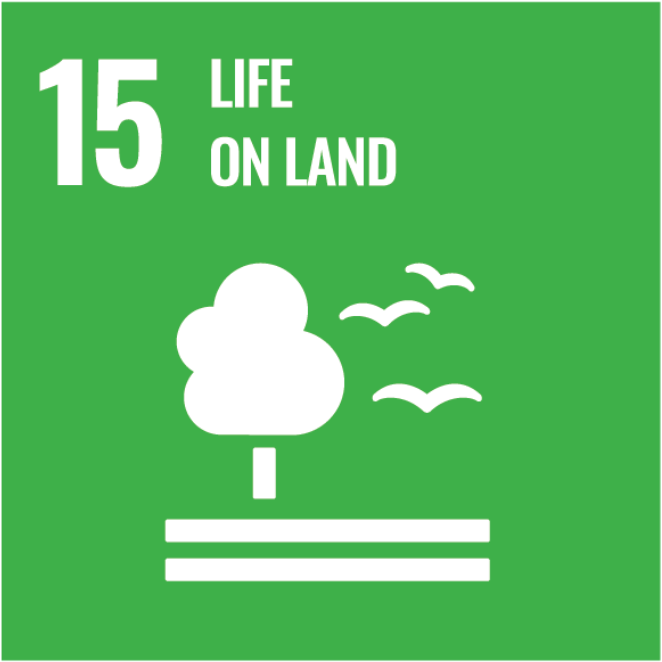
\includegraphics[width=.15\linewidth]{sdg15}

{\parskip=0pt \hypersetup{linkcolor=black}

\tableofcontents

% \chapter*{List of Acronyms}
% 
% \begin{acronym}[ICANN]
%     \acro{lulc}     [LULC]  {Land Use/Land Cover}
%     \acro{ml}       [ML]    {Machine Learning}
%     \acro{al}       [AL]    {Active Learning}
%     \acro{smote}    [SMOTE] {Synthetic Minority Oversampling Technique}
% \end{acronym}
% \addcontentsline{toc}{chapter}{List of Acronyms}

% LIST OF FIGURES
\listoffigures
\addcontentsline{toc}{chapter}{List of Figures}

% LIST OF TABLES
\listoftables
\addcontentsline{toc}{chapter}{List of Tables}
\pagebreak

\chapter*{List of Abbreviations and Acronyms}
{\setstretch{0.5}
\begin{acronym}
    \acro{LULC}         {Land Use/Land Cover}
    \acro{ML}           {Machine Learning}
    \acro{AL}           {Active Learning}
    \acro{SMOTE}        {Synthetic Minority Oversampling Technique}
    \acro{B-SMOTE}      {Borderline-SMOTE}
    \acro{K-SMOTE}      {K-means SMOTE}
    \acro{QBC}          {Query by Committee}
    \acro{EQB}          {Entropy Query-by-Bagging}
    \acro{RQ}           {Research Question}
    \acro{NLP}          {Natural Language Processing}
    \acro{Semi-SL}      {Semi-Supervised Learning}
    \acro{Self-SL}      {Self-Supervised Learning}
    \acro{ROS}          {Random Oversampling}
    \acro{RUS}          {Random Undersampling}
    \acro{DP}           {Differential Privacy}
    \acro{SDV}          {Synthetic Data Vault}
    \acro{MWEM}         {Multiplicative Weights Exponential Mechanism}
    \acro{PGM}          {Probabilistic Graphical Model}
    \acro{HDMM}         {High-dimensional Matrix Mechanism}
    \acro{FTPL}         {Follow-The-Perturbed-Leader}
    \acro{RAP}          {Relaxed Adaptive Projection}
    \acro{RON}          {Random Orthonormal Projection}
    \acro{MST}          {Maximum Spanning Tree}
    \acro{GAN}          {Generative Adversarial Network}
    \acro{CTGAN}        {Conditional Tabular GAN}
    \acro{PATE}         {Private Aggregator of Teacher Ensembles}
    \acro{AE}           {Auto-Encoder}
    \acro{M-Mixup}      {Manifold-Mixup}
    \acro{NL-Mixup}     {Non-linear Mixup}
    \acro{MODALS}       {Modality-Agnostic Automated Data Augmentation in the
                        Latent Space}
    \acro{TVAE}         {Tabular Variational AE}
    \acro{ADASYN}       {Adaptive Synthetic Sampling}
    \acro{G-SMOTE}      {Geometric-SMOTE}
    \acro{MOKAS}        {Minority Oversampling Kernel Adaptive Subspaces}
    \acro{SOM}          {Self-Organizing Map}
    \acro{ASSOM}        {Adaptive Subspace SOM}
    \acro{SOMO}         {SOM Oversampling}
    \acro{G-SOMO}       {Geometric-SOMO}
    \acro{GMM}          {Gaussian Mixture Model}
    \acro{ENN}          {Edited Nearest Neighbors}
    \acro{PDF}          {Probability Density Function}
    \acro{SMOTENC}      {SMOTE for Nominal and Continuous features}
    \acro{VAEACGAN}     {VAE with an Auxiliary-Classifier GAN}
    \acro{STN}          {Spatial Transform Networks}
    \acro{DAE}          {Denoising AE}
    \acro{ICT}          {Interpolation Consistency Training}
    \acro{SDAT}         {Semi-SL Data Augmentation for Tabular Data}
    \acro{MCoM}         {Mixup Contrastive Mixup}
    \acro{VIME}         {Value Imputation and Mask Estimation Method}
    \acro{KL}           {Kullback-Leibler}
    \acro{JS}           {Jensen-Shannon}
    \acro{IR}           {Imbalance Ratio}
    \acro{KNN}          {K-Nearest Neighbors}
    \acro{DT}           {Decision Tree}
    \acro{LR}           {Logistic Regression}
    \acro{RF}           {Random Forest}
    \acro{SVM}          {Support Vector Machines}
    \acro{ANN}          {Artificial Neural Network}
    \acro{ELM}          {Extreme Learning Machines}
    \acro{CV}           {Cross-Validation}
    \acro{BT}           {Breaking Ties}
    \acro{MI}           {Mutual Information}
    \acro{BGDAL}        {Bayesian Generative Active Deep Learning}
    \acro{VAAL}         {Variational Adversarial Active Learning}
    \acro{AULC}         {Area Under the Learning Curve}
    \acro{DUR}          {Data Utilization Rate}
    \acro{OA}           {Overall Accuracy}
\end{acronym}
}
\addcontentsline{toc}{chapter}{List of Abbreviations and Acronyms}
\pagebreak
}



% MAIN THESIS
\setcounter{page}{1}
\pagenumbering{arabic}
\chapter{Introduction}
\graphicspath{{figures/introduction/}}

% Data availability, satellite images
Accurate LULC maps constitute a unique resource for a variety of applications.
Its applications range from environmental monitoring, land change detection,
and natural hazard assessment to agriculture and water/wetland
monitoring~\cite{Khatami2016}. However, the production of LULC maps often
requires the involvement of multiple photo-interpreters with specialized
skills, making the process expensive, time-consuming and unsuitable for
operational LULC mapping over large areas~\cite{Douzas2019rs}. Therefore, the
manual production of LULC maps are often outdated by the time they are
completed, limiting its value to the analysis past conditions in the area of
interest.

An alternative method to address the limitations found in the
photo-interpreted approach to produce LULC maps is automated mapping. This
method uses remotely sensed data, especially multi and hyper-spectral images,
to train ML algorithms to automatically detect the different LULC classes.  To
do this, the usage of recent supervised learning techniques seems to be a
promising path to achieve reliable and updated
maps~\cite{tewkesbury2015critical}. However, the practical application of this
approach is hampered by several limitations: 

\begin{enumerate}
    \item Human error. The quality of the classifiers produced is heavily
        dependent on the quality of its training data. In this case, the
        training dataset is extracted from manually labeled land cover patches
        using typically satellite imagery. The target LULC map's minimum
        mapping unit, as well as the quality of orthophotos and satellite
        images being used are some of the factors that may lead to label noise
        in the training data~\cite{Pelletier2017}.
    \item High dimensionality. The high dimensionality of multi and
        hyper-spectral images contain useful information to improve ML
        classification tasks. However, it also introduces an additional layer
        of complexity and redundancy in classification~\cite{Stromann2020}. If
        the training data is not large enough, it may cause the classification
        task to be affected by the curse of dimensionality.
    \item Class separability. Some LULC classes sometimes contain overlapping
        spectral signatures which makes the separation of the two classes
        particularly challenging in some cases~\cite{Alonso-Sarria2019}.
    \item Infrequent LULC classes. Depending on the region of study, some land
        cover classes may be more or less frequent when compared to other
        regions~\cite{Feng2018}. However, the accurate identification of rare classes
        is often equally or more important than the identification of the
        remaining classes. This problem is known, in ML community, as
        imbalanced learning. As an example, the classification of a desert
        region with 3 classes of interest, bare soil, urban and water, would be
        an imbalanced learning problem. In this case, a classifier that would
        predict bare soil for the entire area of study would have very high
        overall accuracy scores but would not be useful.
    \item Scarcity of labeled data. The increasing number of remote sensing
        missions in the past decades are generating large amounts of high
        quality data. However, only a small portion of this data has some sort
        of LULC ground truth and can be used for supervised learning. In these
        scenarios the production of automated LULC maps is particularly
        challenging and involves the usage of techniques that are able to
        leverage information from both labeled and unlabeled data and
        simultaneously maximize the value of the data annotation
        process~\cite{Simeoni2020}.
\end{enumerate}

The last two challenges, imbalanced learning (\textit{i.e.}, infrequent LULC
classes) and scarcity of labeled data, are the focus of this dissertation.
These two challenges may be addressed in various different ways, all of which
will be discussed throughout the following chapters.

The asymmetry frequently found on LULC class distributions affects the
performance of ML classifiers. In this scenario, during the ML classifier's
learning phase, the minority classes contribute less to the minimization of
accuracy, the typical objective function, biasing the classifier towards the
most frequent classes. The possible approaches to deal with imbalanced
learning can be divided into three main groups~\cite{Fernandez2013}: 

\begin{enumerate}
    \item Cost-sensitive solutions. These methods use a cost matrix to adjust
        the misclassification cost to benefit the minority classes.
    \item Algorithmic-level solutions. These methods introduce algorithmic
        solutions to improve the learning process on the minority classes. 
    \item Resampling solutions. They modify the training data to balance the
        class distribution by removing observations from the majority
        class(es) or adding observations belonging to the minority class(es).
\end{enumerate}

The last set of methods, resampling solutions, benefit from their
simplicity. This type of approach does not require domain knowledge to define
a cost matrix and does not require specialized classifiers. These methods
can be further divided into (1) Oversampling, where an algorithm generates
artificial observations belonging to the minority class, (2) Undersampling,
where an algorithm removes observations belonging to the majority class or (3)
Hybrid approaches, which combine oversampling and undersampling together. In
this thesis, we will focus on oversampling methods and generalize these as a
corner case of augmentation methods for tabular data in later chapters. In
Section~\ref{sec:data_augmentation} this topic is discussed to a greater
extent.

The second challenge discussed in this dissertation is the implementation of
useful ML algorithms in environments with scarce availability of labeled data.
There are three different types of techniques to address this problem, all of
which fall between supervised and unsupervised learning:

\begin{enumerate}
    \item Semi-supervised Learning. Uses both labeled and unlabeled data in
        the training phase to improve the classifier's
        performance~\cite{ouali2020overview}. It pushes the decision
        boundaries of classifiers to regions with lower density of
        observations while maximizing the performance over the labeled
        training dataset~\cite{chapelle2009semi}.
    \item Self-supervised Learning. Uses unlabeled data to perform
        secondary/pretext tasks to learn representations of the input
        space~\cite{grill2020bootstrap}. These methods typically use neural
        network architectures~\cite{liu2021self}.
    \item Active Learning. Iteratively samples the most
        informative/representative observation out of a pool of unlabeled data
        in order to be labeled and included into the training
        dataset~\cite{budd2021survey}. This approach attempts to optimize the
        classifier's performance with as least data as possible.
\end{enumerate}

The last method, Active Learning, benefits from the possibility of including
different techniques into its pipeline, including the former two. It is
therefore one of the main focus of this thesis. In
Section~\ref{sec:active_learning} this topic is discussed to a greater extent.

\section{Data Augmentation}~\label{sec:data_augmentation}

Data Augmentation methods expand the training dataset by introducing new and
informative observations~\cite{Behpour2019}. For this reason, oversampling is
often considered a special case of data augmentation. The production of
artificial data may be done via the introduction of perturbations on the
input~\cite{Zhong2020}, feature~\cite{DeVries2017} or output
space~\cite{Behpour2019}. According to~\citet{Shorten2019} data augmentation
methods may be divided into Heuristic and Neural Network-based approaches. In
addition, they may also be distinguished based on its data generation policy,
whether local (considers a local/specific subset of the dataset) or global
(considers the overall distribution of the training dataset).
Figure~\ref{fig:data_augmentation_taxonomy} shows the general taxonomy of
Heuristic Data Augmentation methods. However, we consider this taxonomy to be
incomplete; a more complete taxonomy is proposed in
Chapter~\ref{chp:synthetic-data-review}. Finding the appropriate Data
Augmentation method generally depends on the domain~\cite{DeVries2017},
whereas few studies discuss which methods are more appropriate according to
the domain~\cite{Shorten2019, Iwana2021, Wong2016}.

\begin{figure}[ht]
	\centering
	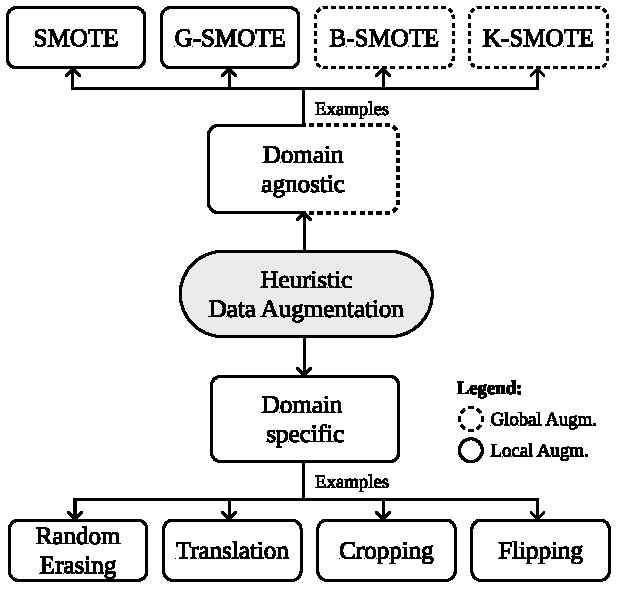
\includegraphics[width=.5\linewidth]{data_augmentation_taxonomy}
    \caption{%
        Schema containing a general Heuristic Data Augmentation taxonomy.
    }~\label{fig:data_augmentation_taxonomy}
\end{figure}

Heuristic approaches attempt to generate new and relevant observations through
the application a predefined procedure, usually incorporating some degree of
randomness~\cite{Kashefi2020}. Since these methods typically occur in the
input space, they require less data and computational power when compared to
Neural Network methods. Neural Network approaches, on the other hand, map the
original input space into a lower-dimensional representation, known as the
feature space~\cite{DeVries2017}. The generation of artificial data occurs in
the feature space and is reconstructed into the input space. Although these
methods allow the generation of less noisy data in high-dimensional contexts
and more plausible artificial data, they are significantly more
computationally intensive. Considering the scope of this thesis, the
computational power available for this experiment and the breadth of datasets
used in the different experimental procedures, we will focus on
domain-agnostic heuristic data augmentation methods.

While some techniques may depend on the domain, others are domain-agnostic.
For example, Random Erasing~\cite{Zhong2020}, Translation, Cropping and
Flipping are image data-specific augmentation methods. Other methods, such as
most of the variants of the Synthetic Minority Oversampling TEchnique
(SMOTE)~\cite{Chawla2002}, may be considered domain agnostic. However, SMOTE
methods were originally developed as oversamplers, whose goal is to balance
the class frequencies of the target variable in the training dataset and
address the class imbalance bias. Therefore, oversampling methods may be
considered a subset of Data Augmentation. Data Augmentation strategies may
follow varying augmentation strategies, which do not necessarily depend on
the target class distribution. An example of the differences among general
data augmentation and oversampling generation strategies is shown in
Figure~\ref{fig:augmentation_strategies}.

\begin{figure}[ht]
	\centering
	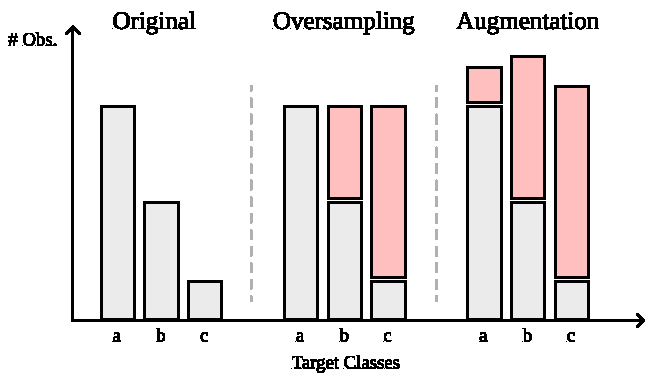
\includegraphics[width=.6\linewidth]{augmentation_strategies}
    \caption[Examples of data augmentation Strategies.]{%
        Examples of data augmentation Strategies. The salmon-colored bars
        represent artificial data using the normal oversampling (center group) and
        an example of augmentation (right group) strategies.
    }~\label{fig:augmentation_strategies}
\end{figure}

The simplest approach found in the literature is randomly duplicating existing
training observations. As a non-informed data generation method, although
simple to implement, it increases the risk of overfitting and generally
performs worse than other informed heuristic
methods~\cite{Douzas2019rs}.

The SMOTE method generates artificial data via the linear interpolation
between a random observation and one of its $k$-nearest neighbors (also
randomly selected)~\cite{Chawla2002}. Although simple and effective, it also
contains several limitations which motivated the development other variants,
discussed below. Specifically, its selection mechanism does not consider the
global structure of the dataset while its generation mechanism introduces
little variability into the training dataset~\cite{Douzas2019}.
Borderline-SMOTE (B-SMOTE)~\cite{Han2005} improves the selection mechanism by
attributing a larger importance to the observations closer to the decision
boundaries. The selected observations are used to run the SMOTE method in
order to produce better defined decision boundaries. A more recent improvement
of the selection mechanism is K-means SMOTE (K-SMOTE)~\cite{Douzas2018}. This
method uses a clustering-based approach to overcome imbalances between and
within classes, while considering the densities of each region of the input
space.

\begin{figure}[ht]
	\centering
	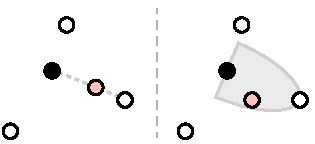
\includegraphics[width=.4\linewidth]{smote_vs_gsmote}
    \caption[Examples of data generation using SMOTE and G-SMOTE\@.]{%
        Examples of data generation using SMOTE and G-SMOTE\@. In this
        example, both G-SMOTE's deformation and truncation parameters assume
        values around $0.5$.
    }~\label{fig:smote_vs_gsmote}
\end{figure}

G-SMOTE~\cite{Douzas2019} modifies SMOTE's generation mechanism. Instead of
generating an observation as a linear combination between 2 others, it
generates observations within an hypersphere defined using the selected
observation as its center and one of its nearest neighbors as its boundary.
The hypersphere contains two hyperparameters, the truncation and deformation
factors, which limit the area of the hypersphere. The difference between SMOTE
and G-SMOTE is shown in Figure~\ref{fig:smote_vs_gsmote}.

\section{Active Learning}~\label{sec:active_learning}

Supervised ML algorithms typically perform well in contexts where labeled data
is abundant and accessible. However, in a practical setting, finding this data
is frequently a challenging task. Depending on the domain, collecting large
volumes of data may not be feasible since the labeling of such data becomes
labor and time intensive and may involve domain experts throughout the
process~\cite{Cao2020}. AL maximizes a classifier's performance while
annotating as least observations as possible. It assumes that observations
within the same dataset have a different contribution to the training of ML
classifiers~\cite{Ren2021}. Consequently, the data annotation cost can be
minimized via the annotation of the most valuable observations within an
unlabeled input space. The goal is to iteratively maximize the classification
performance of ML algorithms while minimizing the required amount of training
data to reach a certain performance threshold~\cite{Shrivastava2021}. It
allows the implementation of ML classifiers with a good performance and
minimal effort when compared to randomly selecting data or labeling the entire
unlabeled dataset~\cite{Ren2021}. Therefore, it addresses the labeling problem
in scenarios with a limited budget, time, or availability of labeled data. 

AL methods may be divided into 2 different stages, initialization and
iteration. Figure~\ref{fig:al_initialization} shows a diagram that represents
the typical AL initialization. Assuming the AL task is initialized without any
previously labeled data, it is typically composed of 3
steps~\cite{Fonseca2021}: 

\begin{enumerate}
    \item Collection of an unlabeled dataset, where the procedure depends on
        the domain of application.
    \item Selection of an initial data subset. Typically, when there is no a
        priori labeled dataset, the initial data subset is randomly picked
        from the unlabeled dataset.
    \item Data labeling. The supervisor is presented with the data subset,
        where its goal is to label each observation. Some of the research
        refers to the supervisor as the oracle~\cite{Yoo2019, Aghdam2019}.
\end{enumerate}

\begin{figure}[ht]
	\centering
	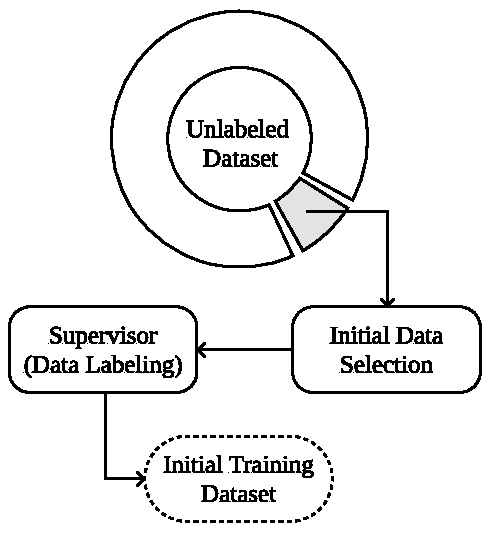
\includegraphics[width=.35\linewidth]{al_initialization}
    \caption{%
        Diagram depicting an AL initialization.
    }~\label{fig:al_initialization}
\end{figure}

Once an initial training dataset is set up, the iterative process of AL takes
place. An AL iteration is completed once a new batch of labeled data is added
to the training dataset. A standard AL process is shown in
Figure~\ref{fig:al_iteration_int} and is composed of the following
steps~\cite{Su2020, Sverchkov2017}:

\begin{enumerate}

    \item Setting up a classification algorithm and uncertainty criterion. The
        classifier is trained using the labeled dataset (\textit{i.e.,} the
        Current Training Dataset), and is used to predict the class membership
        probabilities of the observations found in the unlabeled dataset. The
        class probabilities are passed into an Uncertainty Criterion, which
        will return the classification uncertainty of the classification
        algorithm for each unlabeled observation. The combination of the
        classifier, along with the uncertainty criterion is sometimes referred
        to as the Query/Acquisition function~\cite{Rosario2020}.

    \item Selecting the top N observations. Since it is not possible to
        determine a priori whether the classifier's prediction is correct or
        not, the N observations with highest uncertainty may have been
        unknowingly correctly classified. However, regardless of the
        classification quality, these observations are expected to provide the
        most meaningful information to train the classifier in the next
        iteration.

    \item Labeling the selected N observations and updating the current
        training dataset with the new training observations. The selected
        observations from the unlabeled dataset are presented to the
        supervisor, which is responsible for manually labeling the
        observations. The new (labeled) training observations are added to the
        training dataset and the iteration is completed.

\end{enumerate}

\begin{figure}[ht]
	\centering
	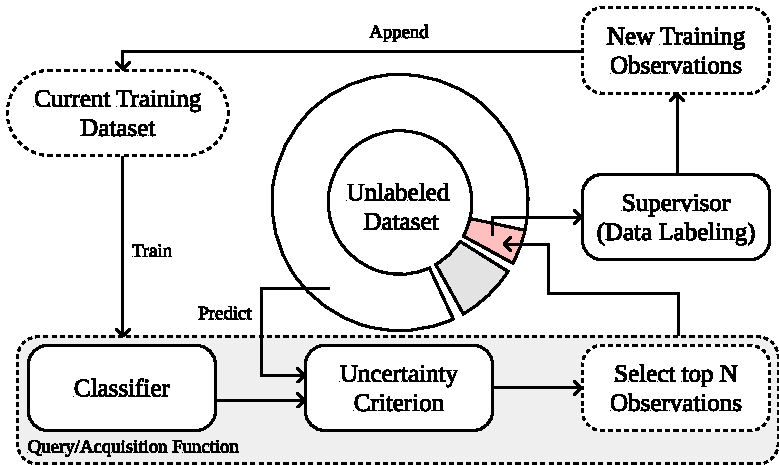
\includegraphics[width=.6\linewidth]{al_iteration}
    \caption[Diagram depicting an AL iteration.]{%
        Diagram depicting an AL iteration. In the first iteration, the
        training set collected during the initialization process becomes the
        ``Current Training Dataset''.
    }~\label{fig:al_iteration_int}
\end{figure}

Two common challenges found in AL implementations are the consistency and
efficiency of AL in practical scenarios~\cite{Kottke2017}. On the one hand,
the consistency problem refers to the high variance in performance (regarding
classification and data selection) over different initializations
(\textit{i.e.,} different initial training datasets) of active learners. On
the other hand, the efficiency problem refers to the maximization of the
quality of the collected data over a run. Therefore, a good active learner is
capable of having a consistent performance over different initializations
while ensuring the production of high-performing classifiers with the least
possible amount of data. There are various factors that may affect the
consistency and efficiency of the AL framework: (1) Human error during data
labeling~\cite{li2020}, (2) Non-informative initial training
dataset~\cite{Nguyen2004} and (3) Lack of an appropriate uncertainty
criterion~\cite{Rosario2020}. AL research has typically been focused on the
specification of uncertainty criteria, as well as domain-specific
applications. Query functions can be divided into two different
categories~\cite{Gu2021, Kumar2020}: 

\begin{enumerate}

    \item Informative-based query strategies. These strategies use the
        classifier's output to assess the importance of each observation
        towards the performance of the classifier. These strategies focus on
        quantifying the class uncertainty of the unlabeled observations.
        Since these techniques do not account for the relationships between
        the unlabeled observations and treats each observation
        independently~\cite{Fu2013}.

    \item Representative-based query strategies. These strategies estimate the
        optimal set of observations that will optimize the classifier's
        performance. This strategy contains 3 main approaches: Density-based,
        Diversity-based and Exploration of graph structures. Although this
        method addresses the problem of sampling bias and redundant instance
        selection, these strategies typically require more observations in
        order to reach the desired classification
        performance~\cite{Kumar2020}.

\end{enumerate}

Although there are significant contributions towards the development of more
robust query functions and classifiers in AL, modifications to AL's basic
structure are rarely explored. In~\cite{Yoo2019} the authors introduce a loss
prediction module in the AL framework to replace the uncertainty criterion.
This model implements a second classifier to predict the expected loss of the
unlabeled observations (using the actual losses collected during the training
of the original classifier) and return the unlabeled observations with the
highest expected loss. Although this contribution is specific to neural
networks (and more specifically, to deep neural networks), they were able to
significantly improve the efficiency of data selection in AL\@.
In~\cite{Simeoni2020} the authors propose the usage of semi-supervised
learning during both the initialization of the AL and the iterative process as
well. However, this method was proposed specifically for deep learning
applications.

A query strategy/function encompasses all the steps prior to the data labeling
within an AL iteration. They focus on finding the observations'
informativeness, representativeness or both~\cite{Gu2021, Kumar2020}.
Representative query strategies are generally less efficient in data selection
than Informative query strategies~\cite{Kumar2020}. However, recent research
often use representative approaches alongside informative
approaches~\cite{Gu2021, Samat2016}. Representative query strategies are
explored via 3 main approaches~\cite{Kumar2020}: 

\begin{enumerate}
    \item Density-based, which select representative observations from high
        density regions.~\cite{Huang2014, Li2012, Ienco2013} used a
        density-based approach using clustering algorithms to select the
        observations closest to the centroid of each cluster. 
    \item Diversity-based, which select the N observations at each iteration
        that maximize the diversity in the training data. The diversity-based
        approach was developed to avoid the selection of redundant
        observations in batch-mode learning~\cite{Brinker2003}.
    \item Graph-based, which find the most representative nodes and edges of a
        graph network~\cite{Jia2019}. Since these methods are specific to
        graph network data, they have a more limited applicability.
\end{enumerate}

Informative query strategies, unlike representative query strategies, do not
account for the structure of the unlabeled dataset. As a result, this type of
strategy may lead to the inefficient selection of observations (\textit{i.e.,}
redundant observations with similar profiles)~\cite{Kumar2020}. Research on
more robust selection criteria attempts to address the efficiency problem.
This is motivated by the importance of the selection criteria in AL's
iterative process~\cite{Rosario2020}. Specifically, Settles~\cite{Settles2011}
observed that in some datasets informative query strategies fail to outperform
the random selection of observations. Generally, the Random Selection query
method is used as a baseline. This method disregards the class membership
probabilities produced by the classifier and returns N random points from the
dataset without following any specific criteria.

A frequently used query strategy is Uncertainty Sampling, originally proposed
in~\cite{Lewis1994}. Using this method, the estimation of an observation's
uncertainty is based on the target class with the highest probability ($p_a$,
according to the classifier) and the uncertainty is calculated as $1-p_a$.
However, since this method dismissed the classifier's predictions on the
remaining labels, the Breaking Ties criterion was proposed to address this
limitation for multiclass problems~\cite{Luo2005}. This method uses the two
target classes with highest probability ($p_a$ and $p_b$, according to the
classifier) and the uncertainty is calculated as $p_a - p_b$ (in this case,
the lower the output value, the higher the uncertainty). Recent variants of
the Breaking Ties criterion, such as the Modified Breaking Ties, attempted to
fix some limitations of the original method~\cite{Liu2018, Li2012a}.

Another common informative query strategy is the calculation of Shannon's
Entropy. This metric measures the level of uncertainty
based on the probabilities of a set of possible events. Its formula is given
by $H(p)=-\sum_{i=0}^n{p_i\log_2{p_i}}$, having $p$ as the set of
probabilities of all target classes. The application of the Entropy
uncertainty criterion is also frequently applied in Deep Active
Learning~\cite{Aghdam2019}. Other Entropy-based methods were also developed
for more specific applications. For example, an ensemble querying approach
known as Entropy Querying-by-Bagging uses the predictions of all estimators to
find the maximum entropy of each observation~\cite{Abe1998}.

The Query by Committee (QBC) strategy was developed to address ensemble
classifiers. It is a disagreement based strategy that attempts to maximize the
information gain at each iteration by computing the disagreement of the
predictions over the estimators that form the ensemble. The Entropy
Querying-by-Bagging and Query-by-Boosting methods are also ensemble
strategies. Query by boosting and bagging methods were found to achieve a good
performance over various datasets~\cite{Melville2004}, while the performance
between the two strategies appears to differ significantly across various
scenarios~\cite{Bloodgood2018}.

Other classifier-specific query strategies were also developed for different
applications. However, these methods have the disadvantage of depending on the
classifier being used. For example, Margin Sampling is a well studied strategy
that uses a Support Vector Machine as its classifier in order to select the
unlabeled observations closest to its decision boundaries~\cite{Kumar2020}.
Although, since this method is known to lead to the excessive selection of
observations in dense regions~\cite{Zhou2014}, it was improved in various
ways. In~\cite{Zhou2014} the authors extend this strategy by applying the
manifold-preserving graph reduction algorithm beyond the normal Margin
Sampling method.


\section{Research Questions}

This dissertation aims to explore and develop new domain-agnostic methods,
leveraged by synthetic data generation techniques, while showing their
effectiveness in difficult classification problems, specifically LULC
classification. The main research questions (RQ) and goals of this
dissertation are the following:

\begin{enumerate}
    \item What are the main research lines in synthetic data generation?
          \begin{itemize}
              \item Development of a literature review to study existing
                  synthetic data generation methods and the core fields where
                  they are being used.
          \end{itemize}
    \item How can one oversample data with both continuous and categorical
        features? 
        \begin{itemize}
            \item Development of an improved oversampling method to be used
                with mixed data types.
        \end{itemize}
    \item How can the quality and consistency of automatic LULC mapping be
        enhanced?
          \begin{itemize}
              \item Exploration of imbalanced learning methods in the context
                  of LULC\@.
          \end{itemize}
    \item How can efficient automated LULC mapping be achieved with limited
        availability of ground-truth data?
        \begin{itemize}
            \item Development of an improved active learning framework in the
                remote sensing domain using artificial data generation.
        \end{itemize}
\end{enumerate}

\section{Main Objectives}~\label{sec:main_objectives}

This research aims to apply and develop new data preprocessing techniques to
LULC classification, with a focus on AL and oversampling techniques. The main
objective is to optimize ML classifiers' performance with minimal labeled data
and/or imbalanced learning scenarios. This objective was decomposed into four
research questions. We start by performing a literature review of synthetic
data generation techniques (RQ1). Second, we propose a new oversampling method
for datasets with both continuous and categorical features (RQ2). Third, we
apply a state-of-the-art oversampling method to understand its effect in LULC
classification tasks (RQ3). Finally, we modify the AL framework to include a
generator and optimize its augmentation policy to reduce the amount of labeled
data required for ML classifiers to reach a satisfactory performance (RQ4).

Each contribution towards the different RQs is divided into different studies.
All chapters refer to a different RQ with the exception
Chapters~\ref{chp:al-generator-lulc}
and~\ref{chp:active-learning-augmentation}, which refer to RQ3. The structure
of this dissertation is shown in Table~\ref{tab:studies}.

RQ1 aims to investigate and consolidate data augmentation methods. This was
done by conducting a literature review to understand the main areas of
application of synthetic data generation and identify the generation
mechanisms available for this purpose. To do this, we conducted an extensive
literature search, compiled the knowledge collected in related literature
reviews, and analyzed several data generation techniques and areas of
application. This approach resulted in a compilation of the most important and
current research in the field, allowing both researchers and practitioners to
use this work as a starting point for their own work. Finally, the development
of this work represents a crucial step to identify new opportunities within
the field and addressing the remaining research questions. The results of this
work is available in Chapter~\ref{chp:synthetic-data-review}.

One of the main limitations uncovered in RQ1 (see
Chapter~\ref{chp:synthetic-data-review}) is the lack of oversampling
methods applicable to datasets containing categorical features. In fact, only
two oversamplers were found to be well-suited for oversampling data with mixed
data types, SMOTENC~\cite{Chawla2002} and random oversampling.  However, in a
practical setting, datasets with mixed feature types are common but the
methods available are outdated. RQ2 is addressed with the modification of a
state-of-the-art oversampling method by mixing its data generation mechanism
with the one found in SMOTENC\@.

Several relevant methods found in Chapter~\ref{chp:synthetic-data-review}
will be used for posterior work. Specifically, we address RQ3 using a
heuristic data augmentation method, K-means SMOTE~\cite{Douzas2018}, as
described in Chapter~\ref{chp:kmeans-smote}. Since datasets produced for LULC
classification often contain irrelevant, redundant, noisy and/or unreliable
data, knowledge discovery is hindered and ultimately leads to the poor
training of predictors. Consequently, data preprocessing becomes an important
contribution to the quality of the predictors developed. In this case, we used
K-means SMOTE to oversample minority regions belonging to the same land cover
class. This was motivated by the challenges faced in producing automated LULC
maps using a training dataset with rare classes. In this scenario, the
spectral signature of a given class often depends on its geographical
distribution and the time of the year the image was captured. Cluster-based
oversamplers, such as K-means SMOTE, allow for a more accurate generation of
minority samples, since it can identify and isolate variations in spectral
signatures within a land cover class.

At a later stage, in RQ4, we addressed a different instance of the problem of
rare land cover classes in the training dataset. Specifically, in a context of
limited sample-collection budget, the collection of the most informative
samples capable of optimally increasing the classification accuracy of a LULC
map is of particular interest~\cite{Su2020}. Active learning attempts to
minimize the human-computer interaction involved in photo-interpretation by
selecting the data points to include into the annotation process. Although,
current state-of-the-art techniques are mostly focused on the improvement of
the acquisition function. We study this problem via the modification of the
typical AL framework. We focus on the usage of data augmentation techniques
and an augmentation policy optimizer to improve the quality of the data
generated. These modifications are presented in
Chapters~\ref{chp:al-generator-lulc}
and~\ref{chp:active-learning-augmentation}:

\begin{itemize}
    \item Chapter~\ref{chp:al-generator-lulc} introduces the generator
        component into the typical AL framework.
    \item Chapter~\ref{chp:active-learning-augmentation} introduces the
        augmentation policy optimizer, while generalizing the generator
        component for augmentation policies beyond oversampling strategies.
\end{itemize}

\section{Methods}

The methodology used for all contributions follows a similar approach, with
exception to the work presented in Chapter~\ref{chp:synthetic-data-review}.
It is composed as follows:

\begin{enumerate}
    \item Collection of a large number of (LULC or multidisciplinary)
        classification datasets.
    \item Identification of related literature and limitations to be addressed.
    \item Design and implementation of contributions.
    \item Definition and implementation of experimental settings.
    \item Analysis of results and statistical significance testing.
    \item Publish results.
\end{enumerate}

The methodological approach to the proposed doctoral work is depicted in
Figure~\ref{fig:phd_structure}. All of the work presented was developed while
ensuring full reproducibility. Contributions at the algorithm-level are
implemented in the Python open-source package 
\href{https://github.com/joaopfonseca/ml-research}{ML-Research}. At the time
of writing, the ML-Research package has been downloaded 12 thousand times via
the Python Package Index (pypi/pip) and Anaconda (conda-forge channel).

\begin{figure}[ht]
	\centering
    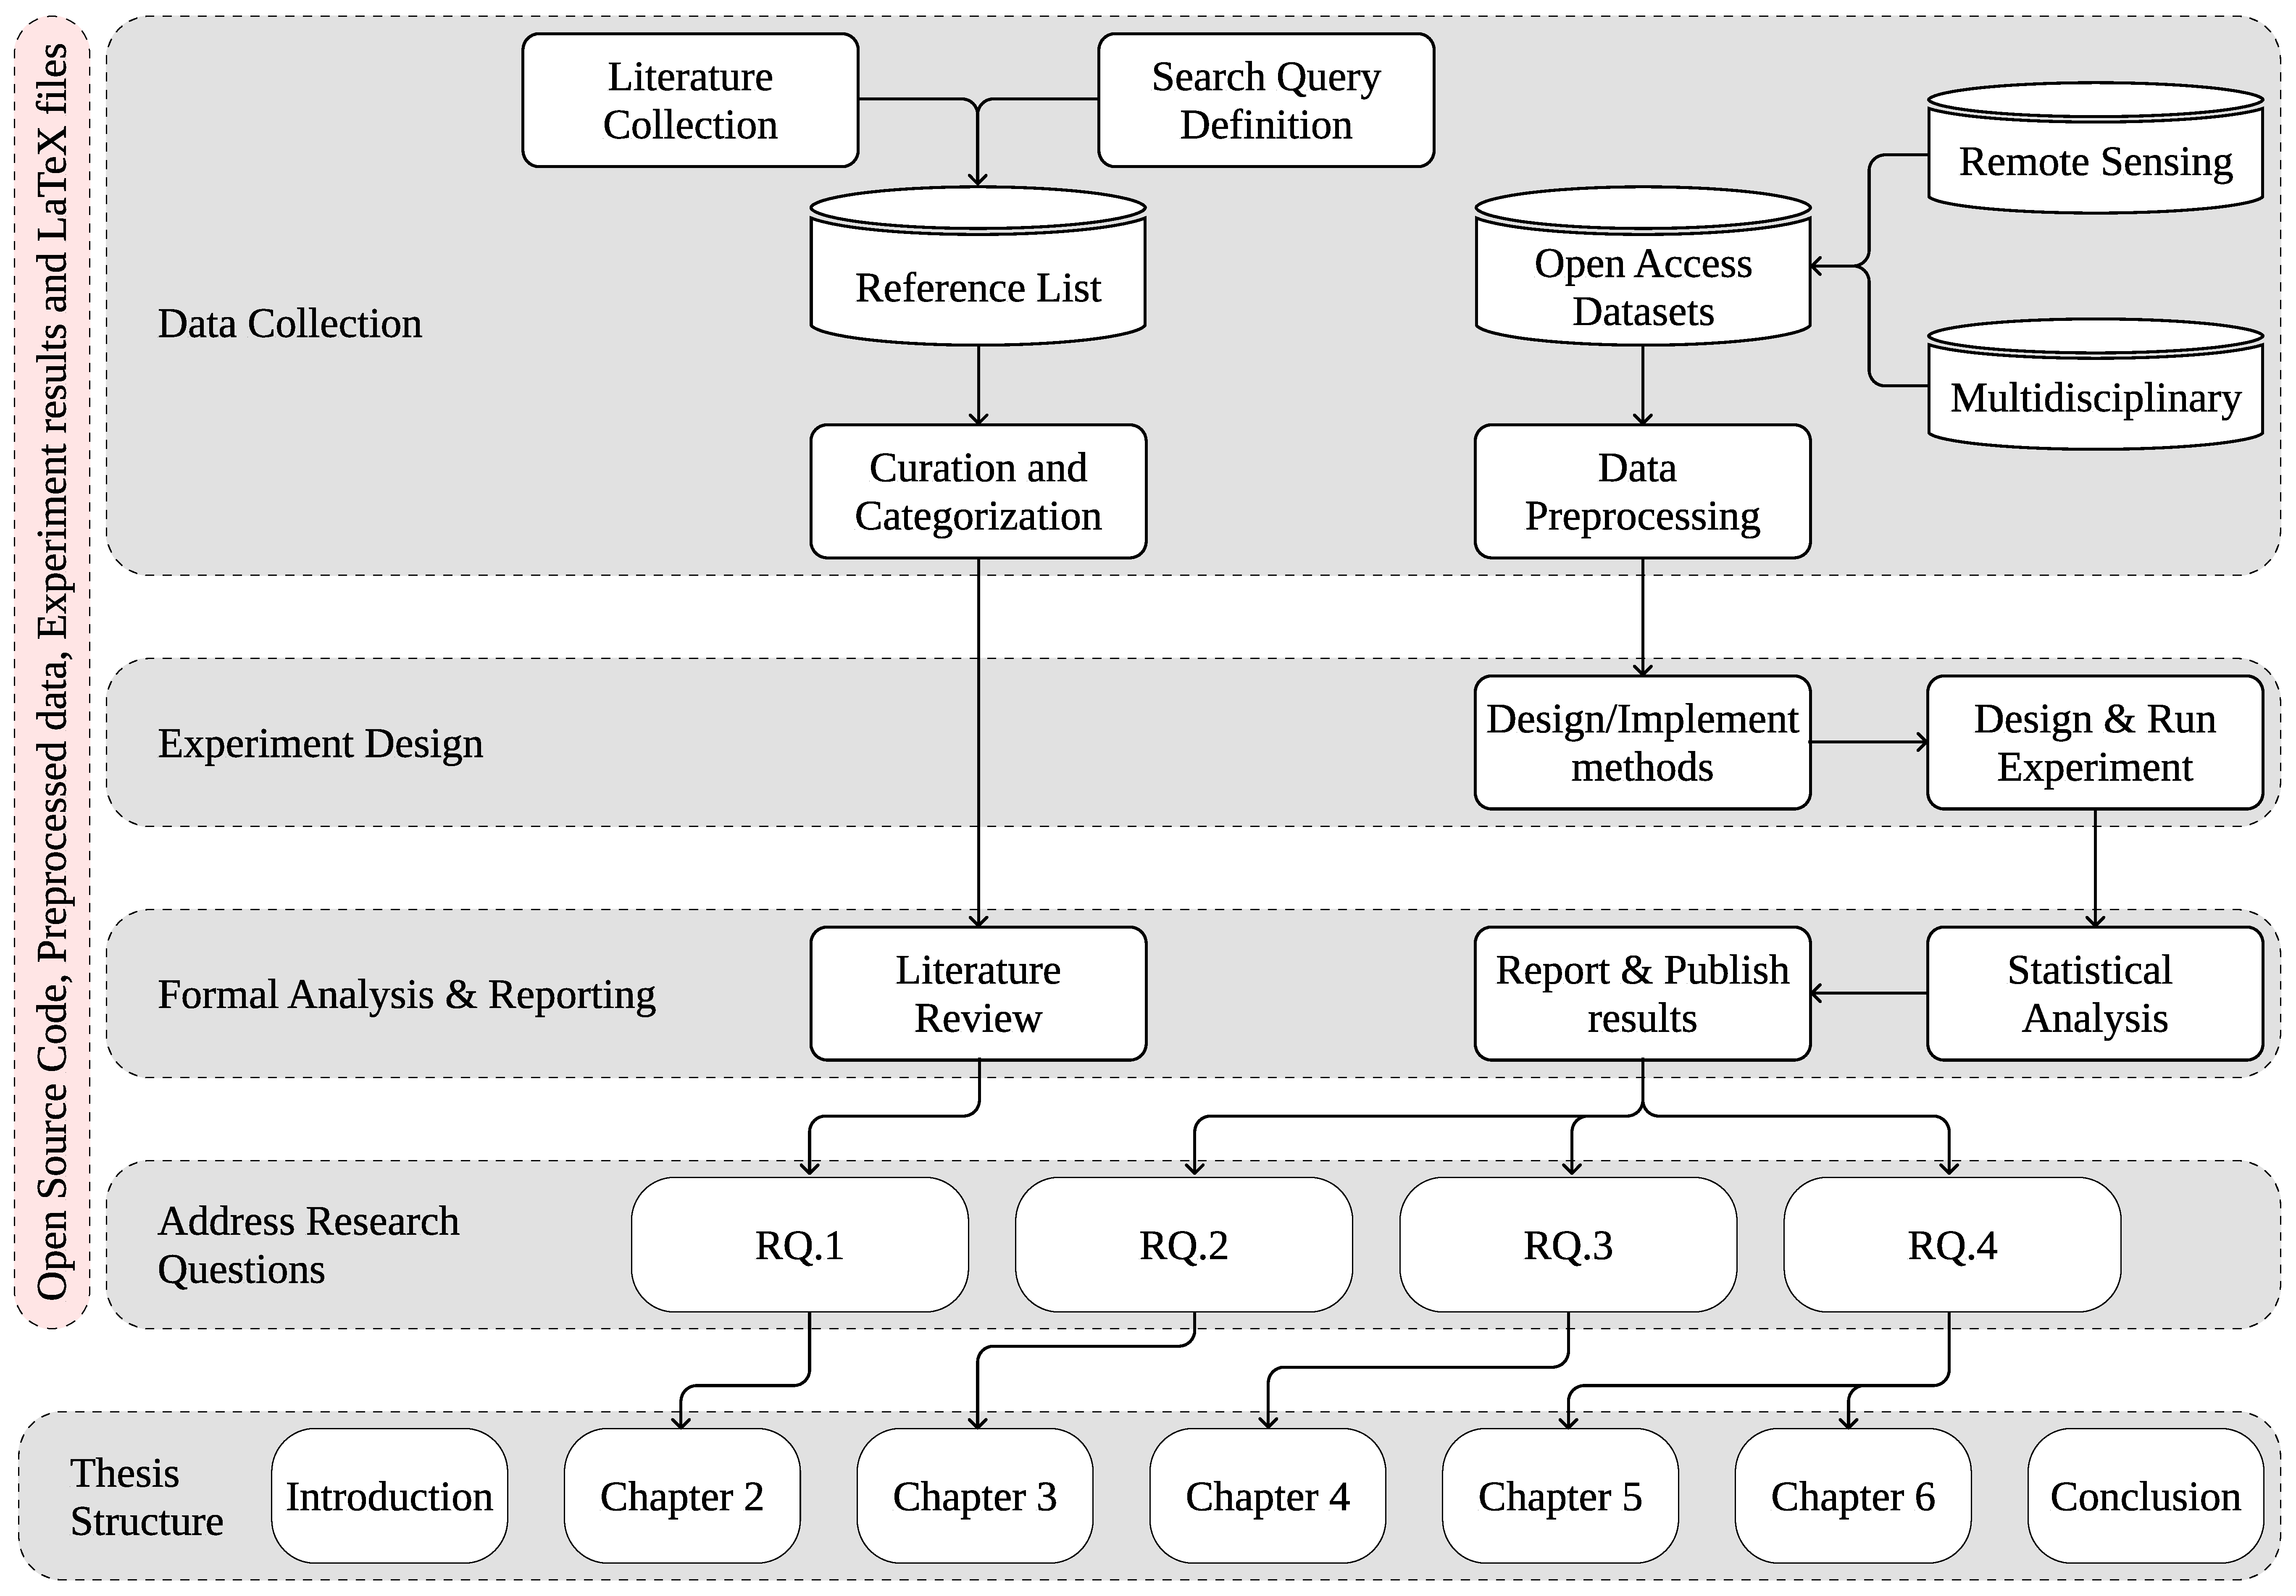
\includegraphics[width=\linewidth]{phd_structure}
    \caption{Structure and methodological approach used in this dissertation.
    }~\label{fig:phd_structure}
\end{figure}


\section{Path of Research}

Each chapter corresponds to a paper (either published or under submission),
all of which primarily focused on AL and imbalanced learning, with exception
to Chapter~\ref{chp:synthetic-data-review}. All of these research outputs are
available at \href{https://github.com/joaopfonseca/publications}{this GitHub
repository}, along with the \LaTeX\ scripts, data, source code (for data
pulling, preprocessing, experiments and analysis), experiments' raw outputs
and analysis outputs (figures, tables and diagrams). The current stage of the
studies is presented in Table~\ref{tab:studies}.

\begin{table}%[ht]
    \centering
    \begin{tabular}{ccm{.55\textwidth}m{.2\textwidth}}
        \toprule
        Chapter & RQ & Study Name                                                        & Current stage  \\
        \midrule
        \ref{chp:synthetic-data-review} & 1    & Tabular and Latent Space
                                                 Synthetic Data Generation: 
                                                 A Literature Review                      & Under Review   \\
        % Research Trends and Applications 
        %                                            of Data Augmentation
        %                                            Algorithms                          & Under Review 
        %                                                                            (Initial submission)  \\
        \vspace{-.2cm}\\
        \ref{chp:gsmotenc} & 2     & Geometric SMOTENC\@: A geometrically
                                     enhanced drop-in replacement for SMOTENC          & Under Review    \\
        \vspace{-.2cm}\\
        \ref{chp:kmeans-smote}             & 3    & Improving Imbalanced Land Cover 
                                                   Classification with K-means SMOTE: 
                                                   Detecting and Oversampling 
                                                   Distinctive Minority Spectral 
                                                   Signatures                          & Published in 
                                                                                         the journal 
                                                                                         Information      \\
        \vspace{-.2cm}\\
        \ref{chp:al-generator-lulc}        & 4    & Increasing the Effectiveness of 
                                                   Active Learning: Introducing
                                                   Artificial Data Generation in 
                                                   Active Learning for Land Use/Land 
                                                   Cover Classification                & Published in 
                                                                                         the journal 
                                                                                         Remote Sensing   \\
        \vspace{-.2cm}\\
        \ref{chp:active-learning-augmentation} & 4 & Improving Active Learning 
                                                   Performance Through the Use of
                                                   Data Augmentation
                                               & Published in International
                                               Journal of Intelligent Systems   \\
        \bottomrule
    \end{tabular}
    \caption{\label{tab:studies}
        Publication stage of the studies developed in the scope of the doctoral
        program.
    }
\end{table}

This dissertation uses synthetic data generation as the core concept
throughout its development. The contributions presented in each chapter
can be split between domain specificity (agnostic versus LULC-specific) and
base technique (oversampling versus AL).
Chapter~\ref{chp:synthetic-data-review} presents a comprehensive literature
review of the central concept of the dissertation, synthetic data generation.
Chapter~\ref{chp:gsmotenc} proposes a domain-agnostic oversampling technique,
to address the problem of datasets with mixed data types (\textit{i.e.},
containing both metric and non-metric features).
Chapter~\ref{chp:kmeans-smote} applies an oversampling technique to LULC
classification problems. Chapter~\ref{chp:al-generator-lulc} proposes an AL
framework using synthetic data generation applied to LULC classification.
Section~\ref{chp:active-learning-augmentation} modifies and improves the
AL framework proposed in the previous chapter and ensure its effectiveness
over several different domains. 

% \thesischapter{%
    Research Trends and Applications of Data Augmentation Algorithms
}{%
    Submitted as Joao Fonseca, Fernando Bacao, to a Q1 Journal, 2022
}~\label{chp:data-augmentation-trends}
\graphicspath{{figures/data-augmentation-trends/}}

\begin{adjustwidth}{30pt}{30pt}

    In the Machine Learning research community, there is a consensus regarding
    the relationship between model complexity and the required amount of data
    and computation power. In real world applications, these computational
    requirements are not always available, motivating research on
    regularization methods. In addition, current and past research have shown
    that simpler classification algorithms can reach state-of-the-art
    performance on computer vision tasks given a robust method to artificially
    augment the training dataset. Because of this, data augmentation
    techniques became a popular research topic in recent years. However,
    existing data augmentation methods are generally less transferable than
    other regularization methods. In this paper we identify the main areas of
    application of data augmentation algorithms, the types of algorithms used,
    significant research trends, their progression over time and research gaps
    in data augmentation literature. To do this, the related literature was
    collected through the Scopus database. Its analysis was done following
    network science, text mining and exploratory analysis approaches. We
    expect readers to understand the potential of data augmentation, as well
    as identify future research directions and open questions within data
    augmentation research.

\end{adjustwidth}

\vspace{.5cm}
\textbf{Keywords:} Data Augmentation; Generative Adversarial Networks; Regularization
Methods; Overfitting

\section{Introduction}~\label{sec:introduction-aug}

The performance of Machine Learning models is highly dependent on the quality
of the training dataset used~\cite{Fenza2021, Halevy2009}. Specifically, the
presence of imbalanced and/or small datasets, target labels incorrectly
assigned, outliers and high dimensional input spaces reduce the prospects of a
successful machine learning model implementation~\cite{Halevy2009,
Domingos2012, Salman2019}.  Even though the performance of any classifier is
affected by the size of its training dataset, deep learning models have a
particularly inconsistent performance over unseen datasets even when trained
with large datasets~\cite{Hu2020, Xie2021}.  Conversely, deep learning models
are capable of quickly adapting (and overfitting) to the training dataset,
including when it contains label and/or complete pixel noise~\cite{Xie2021,
Zhang2021}.  Although the performance of these models can be improved through
regularization methods, they are still incapable of correcting label noise in
the training dataset~\cite{Zhang2021}.

Regardless of the machine learning model used, when the training set contains
significant limitations (regarding overall quality and size), the model's
performance on unseen data is generally going to be affected. Specifically,
when the training data is not representative of the true population, or the
model is over-parametrized, it becomes particularly prone to
overfitting~\cite{Bartlett2021}. There are different strategies to reduce
overfitting, known as regularization methods~\cite{Shorten2019}. Identifying
the appropriate regularization methods varies according to the use
case~\cite{Chun2020}. While some methods can only be applied on specific
classifiers, data types or domains, others may be applied at the data level,
independently from the classification problem. For example, methods such as
dropout/dilution, batch normalization and transfer learning/domain adaptation
are mostly applied on neural network architectures.  Pruning is applied on
decision trees. Early stopping can be used on learners trained iteratively,
making it a broader method. 

Data augmentation techniques are used to increase the size (and hopefully the
diversity) of data in a training dataset through the production of artificial
observations~\cite{Van2001, Wong2016}. They are frequently used as
regularization techniques for various types of problems and classifiers, since
it is applied at the data level~\cite{Behpour2019}.
Figure~\ref{fig:data_augmentation_example} shows an example of data
augmentation, where the decision boundaries become clearer after the original
dataset is augmented. Data Augmentation methods can be divided into heuristic
and Deep Learning approaches~\cite{Shorten2019, Ratner2017}. Within these
approaches, they may be either domain specific or contextually independent.
For example, although both Synthetic Minority Oversampling Technique
(SMOTE)~\cite{Chawla2002} and Kernel Filters are heuristic approaches, SMOTE
may be used regardless of the context, while Kernel Filters are specific to
image data augmentation. The different types of Data Augmentation methods are
defined at a higher detail in Section~\ref{sec:data-augmentation-aug}.

\begin{figure}
	\centering
	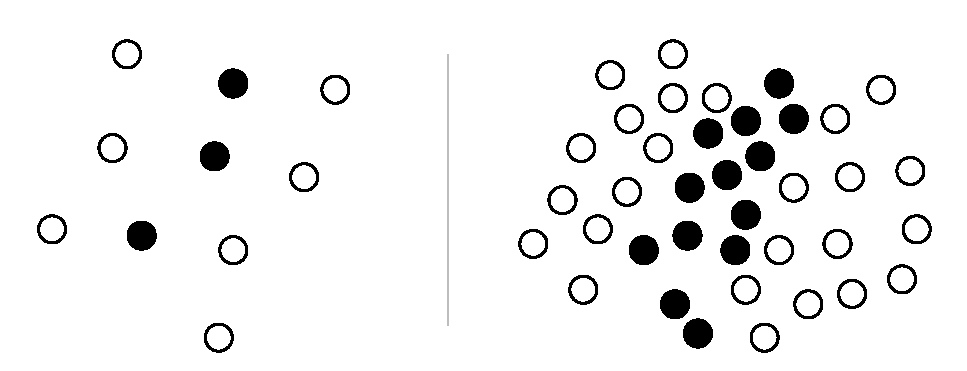
\includegraphics[width=.9\linewidth]{data_augmentation_example}
    \caption[Example of data augmentation in a 2-dimensional binary
    classification setting.]{Example of data augmentation in a 2-dimensional
        binary classification setting. The left pane contains the original
        dataset, where the amount data is scarce and the gap among the two
        classes are wide, allowing for greater classification variability. The
        right pane contains the augmented dataset, where the gap among the two
        classes is narrower and the decision boundaries become easier to
        define.
    }~\label{fig:data_augmentation_example}
\end{figure}

In 2011, Jürgen Schmidhuber's group showed that a MLP ensemble architecture
can achieve state-of-the-art performance on computer vision benchmarks given
strong enough data augmentation~\cite{Meier2011, Ciresan2011}. Although the
state-of-the-art improved since then, two recent papers developed by Google
Brain and Facebook research teams support Schmidhuber's group's findings.
Specifically, in~\cite{Tolstikhin2021, Touvron2021} the authors discuss two
similar MLP ensemble architectures, showing that the proposed model attains a
comparable performance to convolutional neural networks and attention-based
networks. Another recent study also discusses a related MLP architecture with
similar findings, while suggesting that the strong performance of computer
vision models may be attributable mainly to the inducive bias produced by the
patch embedding and the carefully-curated set of training
augmentations~\cite{Melaskyriazi2021}.

Research on data augmentation methods gained significant popularity in recent
years. As such, there were some efforts in the past to establish a taxonomy
and distinction of the different types of data augmentations
methods~\cite{Shorten2019}. To the best of our knowledge, there is no analysis
on data augmentation research as a whole, as well as domains of application
and future directions. In this paper we focus on current and past research
trends of data augmentation methods, its different applications and use cases.
This is done with an extensive analysis of the title, keywords and abstract of
a large set of literature related to data augmentation, collected through the
\href{https://www.scopus.com/}{Scopus} database using Natural Language
Processing and Network Science techniques. The analysis contains 3 phases. We
started by performing an exploratory data analysis to identify the most
significant publications, journals and conferences within the field of data
augmentation. Then, we analysed the articles' author keywords by constructing
a network and extracting and identifying communities of keywords.  Finally we
used a text mining approach to extract additional applications and methods
using the articles' abstracts, as well as validate the findings discussed with
the keyword analysis.

The rest of this paper is structured as follows:
Section~\ref{sec:data-augmentation-aug} describes the main methods and approaches
used in data augmentation, Section~\ref{sec:methodology-aug} describes the
procedures defined throughout the different analyses.
Section~\ref{sec:results_discussion-aug} presents and discusses the findings drawn
from the analyses, as well as research gaps and open questions in data
augmentation research. Section~\ref{sec:conclusion-aug} summarizes the main
findings discussed throughout the study.

\section{Data Augmentation Methods}~\label{sec:data-augmentation-aug}
 
Based on the literature found, a Data Augmentation method may be characterized
based on 3 criteria. The more common division is done between Heuristic and
Deep Learning approaches~\cite{Shorten2019}. Within these, several approaches
have been developed to produce artificial observations at the
input~\cite{Zhong2020}, feature~\cite{DeVries2017}, or output
space~\cite{Behpour2019}. Finally, we also distinguish them based on whether
their generation mechanism considers local (\textit{i.e.,} considers
partial/specific information within the dataset) or global (\textit{i.e.,}
it's based on the overall distribution/structure of the dataset) information
of the original dataset. Figure~\ref{fig:concept_map} depicts the concept map
with the different subdivisions of characteristics of data augmentation
methods. In this section, the analysis of the different types of data
augmentation will be based on their architectural approach. However, all the
methods mentioned may be divided using any of the definitions mentioned.

\begin{figure}[htb]
	\centering
	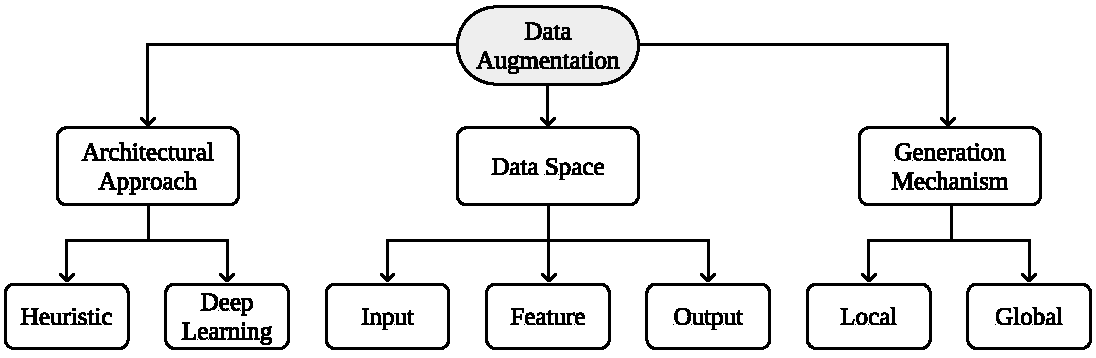
\includegraphics[width=\linewidth]{concept_map}
    \caption{%
        Data Augmentation concept map.
    }~\label{fig:concept_map}
\end{figure}

Heuristic methods use the information found in the input space to generate
new, relevant, non-duplicated observations by applying a predefined set of
rules, while incorporating a degree of randomness in the generation process.
Since data augmentation occurs in the input space, these are cost-effective
approaches to data augmentation. For this reason, heuristic methods are
simpler to implement and are particularly appealing for low dimensional
classification problems, especially when the computational power available is
limited. 

Some Deep Learning methods, on the other hand, attempt to map the original
input space into a lower-dimensional representation, known as feature
space~\cite{DeVries2017}. The generation of artificial observations occurs at
the feature space level, before being reconstructed to the original input
space. This is commonly done with Convolutional Neural Networks (CNN) and
auto-encoder architectures~\cite{Shorten2019}. Since data augmentation is
performed in the feature space, this type of approach is particularly useful
for high-dimensional data types and results in more plausible synthetic
observations~\cite{DeVries2017}. However, deep learning approaches require
more computational power than heuristic approaches and the resulting feature
space is difficult to interpret.

The difference in classification performance of the two perspectives is still
unclear. Wen et al.~\cite{Wen2020} evaluate the impact of data augmentation on
time series for various classification and forecasting tasks. Although they
found that both heuristic and deep learning approaches improved the results
over the various experiments, there was no direct comparison among the
different methods. Wong et al.~\cite{Wong2016} compared both input and feature
space data augmentation methods for image data classification performance over
the MNIST dataset. They found that input space augmentation can lead to better
classification performance if plausible transforms on the data are known.
However, in~\cite{DeVries2017} the authors discuss that the effectiveness of
each data augmentation method generally depends on the domain. The lack of
research on effective, domain-agnostic data augmentation methods appears to be
a current research gap.

\subsection{Heuristic Approaches}

Various heuristic approaches depend on the data type. For example, image data
augmentation may be done via translation, cropping or random
erasing~\cite{Zhong2020}, among others~\cite{Shorten2019}. However, these
techniques depend on the context and may not be applicable to other data types
such as time-series~\cite{Wen2020, Iwana2021} or tabular data. In this
subsection we will focus on domain-agnostic data augmentation methods.

Heuristic approaches may be applied at the input or feature space. The
appropriate method to be applied also depends on the machine learning goal.
Specifically, heuristic methods are commonly used to address classification
problems where the frequency of the different target classes vary
significantly, a problem known as Imbalanced Learning~\cite{Chawla2004}. In
this context, the dataset contains one or multiple rare classes, which become
more difficult to predict. This happens because during the learning phase,
classifiers are trained in order to maximize one or few performance metrics.
Although, a poor choice of performance metrics (\textit{i.e.}, a metric
insensitive to class imbalance, such as overall accuracy) might lead to a poor
estimation of the model's actual performance, since minority classes
contribute less to the learning phase and to the estimation of the performance
metric~\cite{Fonseca2021}. 

The problem of Imbalanced Learning is frequently addressed with oversampling
algorithms~\cite{Kaur2019}. Oversampling methods generate artificial
observations in order to balance class distributions using contextual
information based on the original dataset. These methods apply linear or
geometric interpolations between a random observation and one of its neighbors
to generate a new observation.

SMOTE~\cite{Chawla2002} is one of the most popular oversampling methods. It
generates an artificial observation along a line segment between a randomly
selected minority class observation and one of its nearest-neighbors. Since it
was first proposed, modifications at the neighbors parent observations
selection and data generation mechanisms of the original algorithm were
proposed. Borderline-SMOTE~\cite{Han2005} is an example of a modification of
SMOTE's data selection mechanism. Instead of selecting any random minority
class observation and one of its neighbors, the algorithm focuses in the
minority class observations closest to the decision boundary.
Geometric-SMOTE~\cite{Douzas2019} proposes a modification of the data
generation mechanism. Instead of generating data within a line segment, it
generates data within a hyper-spheroid between two parent observations.

Contrary to Deep Learning approaches, heuristic approaches can be applied at
the input space without the need of learning a feature space. This allows the
implementation of heuristic data augmentation with less computational power
and technical complexity. In addition, in contexts of limited data
availability (\textit{i.e.}, small datasets), deep learning approaches are not
appropriate since the amount of parameters to be tuned during the learning
phase often exceeds the number of observations in the dataset, making it
over-parametrized. The augmentation of small datasets using heuristic
approaches is explored in an Active Learning context
in~\cite{Fonseca2021al}. The authors found that significantly smaller
amounts of curated data using Active Learning, along with heuristic data
augmentation methods, achieved a classification performance comparable to
classifiers trained over the full dataset.

\subsection{Deep Learning Approaches}

Different deep learning approaches and architectures have been developed for
various domains. Deep learning data augmentation methods may be developed via
augmentation at the feature space (which involves learning a feature
space)~\cite{DeVries2017} or via a combination of a set number of observations
into a neural network in order to output a non-linear, non-geometric
combination of input observations~\cite{Wang2017}. Other domain-specific deep
learning methods also exist, such as style transferring techniques (specific
to image data)~\cite{Wang2017, Zhu2017}.

Data augmentation at the feature space is especially useful when dealing with
high-dimensional datasets with complex and/or discontinuous distributions.
For example, many heuristic data augmentation techniques cannot be applied in
handwritten digits classification problems since they may change the true
label of the generated image and generate noisy data. In this situation,
performing data augmentation at the input space may introduce
noise~\cite{Chu2020}, since the data is also subjected to the curse of
dimensionality (see Figure~\ref{fig:input_vs_feature_space}a). This allows
transformations of known observations in a lower dimensional space to generate
new, non-noisy artificial observations projected in the input space, as shown
in Figures~\ref{fig:input_vs_feature_space}b
and~\ref{fig:input_vs_feature_space}c. 

\begin{figure}[htb]
	\centering
	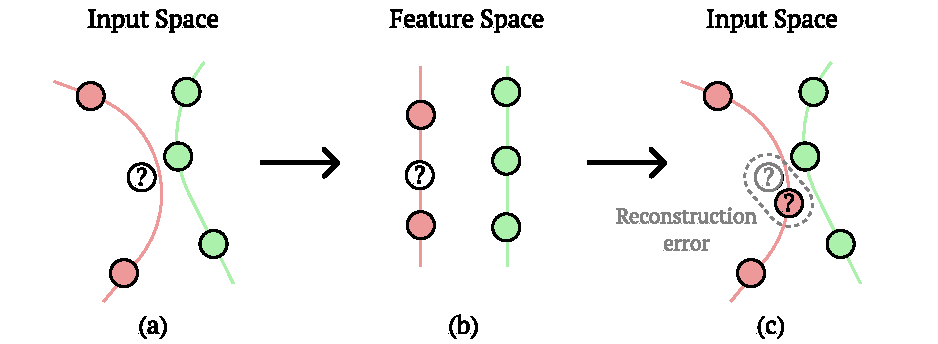
\includegraphics[width=.9\linewidth]{input_vs_feature_space}
    \caption[Example of a sparse input space and its corresponding feature
    space.]{%
        Example of a sparse input space and its corresponding feature space.
        Learning a manifold feature space facilitates the generation of
        non-noisy artificial data. In the original input space (a) the
        unseen/artificial observation marked with ``?'' is closer to a green
        observation and to the learnt red manifold space, which may lead to a
        noisy observation. When projected or generated in the feature space
        (b), the observation will better match the nearest manifold measure
        and avoid noisy data in the input space (c). Adapted
        from~\cite{Antoniou2017}.
    }~\label{fig:input_vs_feature_space}
\end{figure}

The utilization of autoencoders~\cite{Kramer1991} is particularly useful to
perform feature space data augmentation~\cite{Shorten2019}. Autoencoders are
composed by an encoder and a decoder, which map the input space to and from
the feature space, respectively. The autoencoder is trained by minimizing the
difference between the original observation and the reconstructed observation
(see Figure~\ref{fig:input_vs_feature_space}c). Once the training phase is
completed, heuristic methods are applied in the feature
space~\cite{DeVries2017}.

Generative Adversarial Network (GAN)~\cite{Goodfellow2014} architectures is a
deep learning approach frequently used as a data augmentation method. It
involves a generator and a discriminator. Although many different
architectures have been proposed, the generator in the vanilla GAN algorithm
may be seen as a decoder, which is trained based on the gradients calculated
via the discriminator. The discriminator attempts to distinguish true and
generated (fake) observations in order to assess the quality of the data
produced by the generator. The problem is better formulated as a minimax
decision rule, where the generator attempts to fool the discriminator by
producing observations that are difficult to classify as generated.

When the size of the training dataset is not sufficiently large to employ deep
learning approaches and other related datasets or unlabeled datasets are
available, one technique that may also be used is transfer learning. In this
context, the data augmentation model is trained on a secondary model and is
later adjusted to the training dataset. This allows the usage of deep learning
models in few-shot learning environments~\cite{Antoniou2017}.

\section{Methodology}~\label{sec:methodology-aug}

In this section we describe the procedures defined for the literature
collection, data preprocessing and literature analysis. The analysis of the
literature was developed with 3 different approaches. Throughout the
analyses, data preprocessing and hyperparameter tuning was developed
iteratively. The procedure adopted in this manuscript is shown in
Figure~\ref{fig:slr_diagram}.

The literature collection procedure is described in
Subsection~\ref{sec:lit_collection-aug}. The data and text preprocessing is
described in Subsection~\ref{sec:data_preprocessing-aug}. The exploratory data
analysis described in Subsection~\ref{sec:journal_and_conference_analysis-aug} was
done to understand which manuscripts, journals and conferences are most
significant within the field of Data Augmentation. The manuscripts' keywords
were used to construct a network of keywords (described in
Subsection~\ref{sec:keyword_analysis-aug}) and study the different communities of
keywords found in the network. The topic modelling and parameter tuning is
described in Subsection~\ref{sec:topic_modelling-aug}. 

\begin{figure}
	\centering
	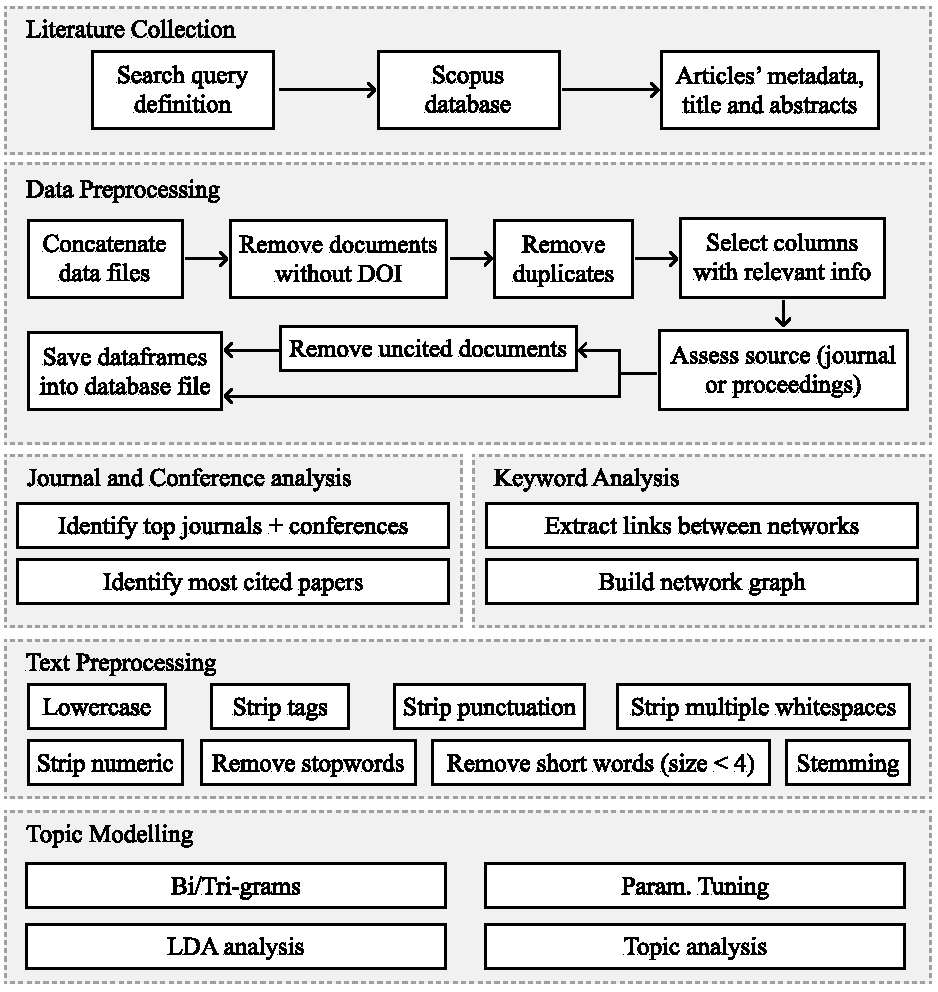
\includegraphics[width=.85\linewidth]{slr_diagram}
    \caption{Diagram of the proposed literature analysis approach.
    }~\label{fig:slr_diagram}
\end{figure}

\subsection{Literature Collection}~\label{sec:lit_collection-aug}

The focus of this literature analysis is to understand the different
algorithms, domains and/or tasks that employ data augmentation techniques.
Therefore, we search for documents containing the keyword ``data
augmentation'' in the search query. The results were then limited to
conference papers and journal articles written in English that were published
in the past 15 years.  Due to the large amount of results found, using solely
the \href{https://www.scopus.com/}{Scopus} database was found to be
sufficient. One of the goals during the search query design was to come up
with a simple and unbiased query. The resulting query is shown below:

\begin{verbatim}
    KEY ("data augmentation") AND (LIMIT-TO (LANGUAGE, "English"))  
    AND (LIMIT-TO (DOCTYPE, "cp") OR LIMIT-TO (DOCTYPE, "ar"))  
    AND (LIMIT-TO (PUBYEAR, 2021) OR LIMIT-TO (PUBYEAR, 2020)  
     OR  LIMIT-TO (PUBYEAR, 2019) OR LIMIT-TO (PUBYEAR, 2018)  
     OR  LIMIT-TO (PUBYEAR, 2017) OR LIMIT-TO (PUBYEAR, 2016)  
     OR  LIMIT-TO (PUBYEAR, 2015) OR LIMIT-TO (PUBYEAR, 2014)  
     OR  LIMIT-TO (PUBYEAR, 2013) OR LIMIT-TO (PUBYEAR, 2012)  
     OR  LIMIT-TO (PUBYEAR, 2011) OR LIMIT-TO (PUBYEAR, 2010)  
     OR  LIMIT-TO (PUBYEAR, 2009) OR LIMIT-TO (PUBYEAR, 2008)  
     OR  LIMIT-TO (PUBYEAR, 2007) OR LIMIT-TO (PUBYEAR, 2006))  
\end{verbatim}
\bigskip

The search query resulted in 4281 documents. The resulting data
selection/filtering pipeline is shown in
Figure~\ref{fig:data_filtering_pipeline}. Due to the limitations in the Scopus
data export (maximum 2000 documents per export), the data was split in four
different time periods and exported separately: 2006 until 2018, 2019, 2020
and 2021, which produced four CSV files.

\subsection{Data Preprocessing}~\label{sec:data_preprocessing-aug}

The data preprocessing stage and amount of documents dropped is represented in
Figure~\ref{fig:data_filtering_pipeline}. The data was first concatenated into
a single data frame. During this process, we found that one of the exported
references had a corrupted line, which caused the loss of one additional
document.  Since the DOI can be used as a unique identifier for intellectual
property~\cite{Paskin1999}, references without a DOI were disregarded from
further analysis, while the ones with the same identifiers are removed
(\textit{i.e.}, only one of the repeating entries is kept).

This dataset was kept to perform the analysis described in
Subsection~\ref{sec:journal_and_conference_analysis-aug}. However, further
preprocessing was done for the remaining parts of the literature analysis.
References without any citations were excluded for the keyword network and
topic modelling analyses. Finally, only the documents containing keywords in
Scopus' database were used to prepare the network analysis.

\begin{figure}
	\centering
    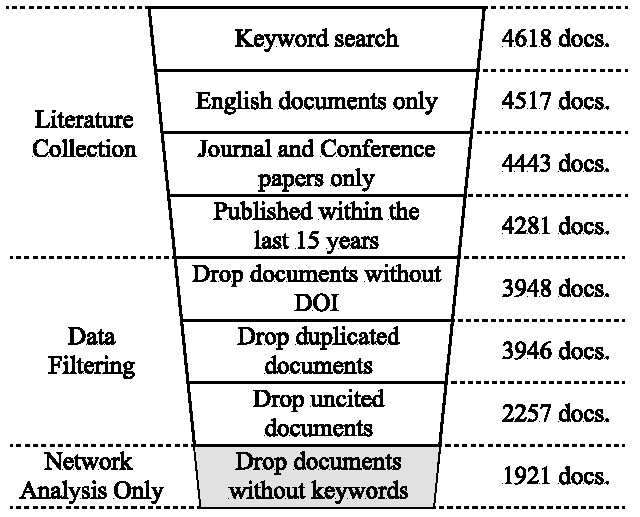
\includegraphics[width=.6\linewidth]{data_filtering_pipeline}
    \caption{Data filtering pipeline.
    }~\label{fig:data_filtering_pipeline}
\end{figure}

\subsection{Journal and Conference
analysis}~\label{sec:journal_and_conference_analysis-aug}

The exploratory analysis developed on the preprocessed dataset was targeted
towards the identification of the most significant works, journals and
conferences. We used the citation count as a proxy to understand the impact of
a specific manuscript within the research community.

The identification of the most significant conferences and journals is done by
sorting each type of publication according to the number of citations per
document. Conferences and journals with less than 10 papers published in the
area are not considered in this analysis. 

\subsection{Keyword Analysis}~\label{sec:keyword_analysis-aug}

The analysis of keywords is expected to uncover general trends in data
augmentation research and its applications. The keyword ``data augmentation''
was removed since it would link with all other keywords. Keywords are
connected based on their co-occurrence in each research paper to form the
edges of the network.  It consists of an undirected graph whose weights are
based on the total citation count for the papers containing a given keyword
pair and is calculated as $\textrm{weight} = \log(\textrm{citations}) + 1$ to
avoid a potential bias caused by highly cited research articles. The size of
the nodes were determined with a logarithmic transformation of each
node's page rank.

Keyword combinations showing up in only one document are removed from further
analysis. The keyword network is then analysed using Python and the
communities were found using the greedy modularity maximization algorithm
proposed in~\cite{Clauset2004}. The results of the analysis and community
detection were ported to Gephi to produce the final visualizations.

\subsection{Topic Modelling}~\label{sec:topic_modelling-aug}

The extraction of topics was done using the publication's abstracts. The words
were tokenized and all tags, special characters, punctuation, multiple white
spaces, numeric values, stop words and words with size smaller than 4 were
removed. Finally, we enriched the corpus by constructing bi-grams and
tri-grams.

We used a Latent Dirichlet Allocation (LDA) model~\cite{Pritchard2000} to
infer the topics present in our research domain. The tuning of the parameters
was done through experimentation and qualitative interpretation of the results
achieved. Additionally, the coherence score curve was also used as a reference for
parameter tuning and the choice of parameters, which are described in
Table~\ref{tab:hyperparameters}. 

\begin{table}[ht]
    \begin{center}
    \begin{tabular*}{.5\textwidth}{@{\extracolsep{\fill}}lllllll@{\extracolsep{\fill}}}
        \toprule
        Model   &   Hyperparameter  &   Value \\
        \midrule
        LDA     &   Num Topics      &   8     \\
                &   Chunk Size      &   2000  \\
                &   Passes          &   20    \\
                &   Alpha           &   0.1   \\
                &   ETA             &   auto  \\
        \bottomrule
    \end{tabular*}
    \caption{Hyperparameters used.}~\label{tab:hyperparameters}
    \end{center}
\end{table}

\subsection{Software Implementation}~\label{sec:software_implementation-aug}

The analysis and modelling was developed using the Python programming
language, along with the
\href{https://scikit-learn.org/stable/}{Scikit-Learn}~\cite{Pedregosa2011},
\href{https://radimrehurek.com/gensim/}{Gensim}~\cite{Rehurek2010}, and
\href{https://networkx.org/}{Networkx}~\cite{Hagberg2008} libraries. The final
network analysis and visualization was done with
\href{https://gephi.org/}{Gephi}~\cite{Bastian2009}. All functions,
algorithms, analyses and results are provided in the
\href{https://github.com/joaopfonseca/publications}{GitHub repository of the
project}.

\section{Results \& Discussion}~\label{sec:results_discussion-aug}

The popularity of research in data generation has grown significantly in the
past 5 years, as shown in Figure~\ref{fig:area_chart_cited_documents}. Despite
the significant amount of uncited publications, out of the ones published in
2020, 39\% have already been used in other works. Although most of the
research developed before 2016 was used in other works, the amount of cited
research increased significantly after that period.

\begin{figure}
	\centering
    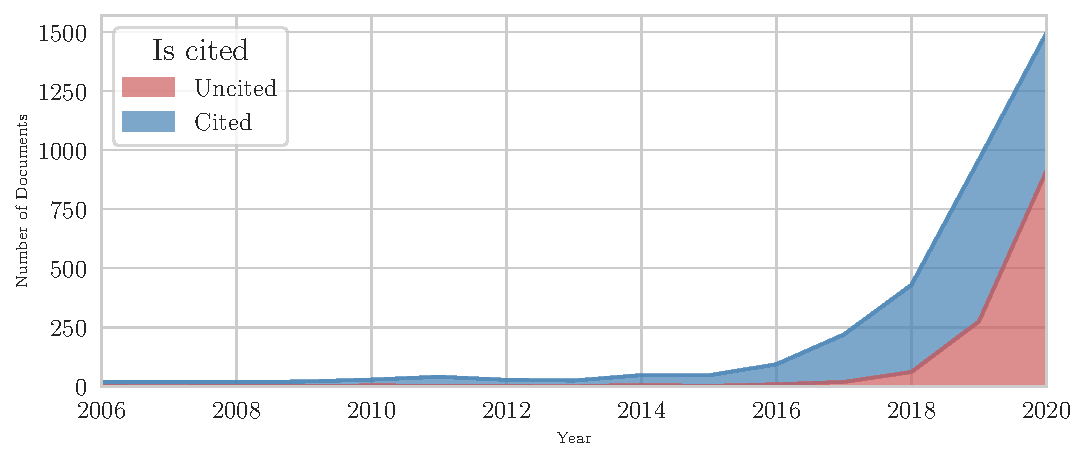
\includegraphics[width=\linewidth]{area_chart_cited_documents}
    \caption{Annual number of publications containing the keyword ``data
        augmentation''.
    }~\label{fig:area_chart_cited_documents}
\end{figure}

\subsection{Journal and Conference Analysis}

The initial exploration of the bibliometric data allows us to assess which
journals focused in data augmentation more intensely over the past years, as
shown in Table~\ref{tab:top_journals}. Most of the top journals belong to
technical fields, predominantly from Statistics, Remote Sensing, Medical
Imaging and other domains of applications such as agriculture. In addition,
all these journals have a high impact in their respective fields (based on
\href{https://www.scimagojr.com/}{Scimago Journal \& Country Rankings}).   

\begin{table}[ht]
    \begin{center}
    \begin{tabular*}{\textwidth}{@{\extracolsep{\fill}}lllllll@{\extracolsep{\fill}}}
        \toprule
        Source title & Publications & Citations & Average \\
        \midrule
        Journal of the American Statistical Association & 11 & 538 & 48.91 \\
        IEEE Geoscience and Remote Sensing Letters & 19 & 552 & 29.05 \\
        Neurocomputing & 35 & 808 & 23.09 \\
        Expert Systems with Applications & 14 & 283 & 20.21 \\
        Medical Image Analysis & 15 & 288 & 19.20 \\
        Neural Networks & 10 & 190 & 19.00 \\
        Journal of Computational and Graphical Statistics & 23 & 433 & 18.83 \\
        Computers and Electronics in Agriculture & 15 & 219 & 14.60 \\
        Biometrics & 13 & 163 & 12.54 \\
        IEEE Transactions on Medical Imaging & 10 & 123 & 12.30 \\
        \bottomrule
    \end{tabular*}
    \caption[Top journals focusing on data augmentation techniques]{%
        Top journals focusing on data augmentation techniques, sorted by
        citations per document.
    }~\label{tab:top_journals}
    \end{center}
\end{table}

Citation-wise, the publications coming from conference proceedings tend to
have a comparable impact in the research community, as shown in
Table~\ref{tab:top_conferences}. The most relevant conferences are positioned
in the computer science and information management fields. Research developed
in other areas of application, such as computer vision, speech recognition,
acoustic modelling, natural language processing and signal processing have
more activity in the form of conference proceedings publications. Conversely,
the domains most frequent in journal publications are not as active on
conference proceedings publications.

\begin{table}[ht]
    \begin{center}
    \begin{tabular*}{\textwidth}{@{\extracolsep{\fill}}lllllll@{\extracolsep{\fill}}}
        \toprule
        Source title & \# Pubs. & Cited & Avg \\
        \midrule
        Proceedings of the IEEE Computer Society Conference & 49 & 2111 & 43.08 \\
        \vspace{.2cm}on Computer Vision and Pattern Recognition &&& \\
        Lecture Notes in Computer Science (including subseries & 372 & 14946 & 40.18 \\
        Lecture Notes in Artificial Intelligence and Lecture Notes &&& \\ 
        \vspace{.2cm}in Bioinformatics) &&& \\

        \vspace{.2cm}Procedia Computer Science & 13 & 288 & 22.15 \\

        International Conference on Information and Knowledge & 10 & 180 & 18.00 \\
        \vspace{.2cm}Management, Proceedings &&& \\

        IEEE Computer Society Conference on Computer Vision & 23 & 314 & 13.65 \\
        \vspace{.2cm}and Pattern Recognition Workshops &&& \\

        ICASSP, IEEE International Conference on Acoustics, & 95 & 1153 & 12.14 \\
        \vspace{.2cm}Speech and Signal Processing - Proceedings &&& \\

        Proceedings - International Symposium on Biomedical & 30 & 346 & 11.53 \\
        \vspace{.2cm}Imaging &&& \\

        Proceedings of the International Conference on Document & 17 & 158 & 9.29 \\
        \vspace{.2cm}Analysis and Recognition, ICDAR &&& \\

        Proceedings of International Conference on Frontiers & 13 & 113 & 8.69 \\
        \vspace{.2cm}in Handwriting Recognition, ICFHR &&& \\

        2019 IEEE Automatic Speech Recognition and & 12 & 84 & 7.00 \\
        Understanding Workshop, ASRU 2019 - Proceedings &&& \\
        \bottomrule
    \end{tabular*}
    \caption[Top conferences focusing on data augmentation techniques]{%
        Top conferences focusing on data augmentation techniques, sorted by
        citations per document.
    }~\label{tab:top_conferences}
    \end{center}
\end{table}

The papers with the highest citation count are listed in
Table~\ref{tab:top_papers}. We found that much of the research focused on
improving deep learning classification, segmentation or object detection
without a focus on a particular domain of application. Other papers centered
in the application of data augmentation methods for biomedical image
classification and segmentation, sound and speech recognition and remote
sensing.

\begin{table}[ht]
    \begin{center}
    \begin{tabular*}{\textwidth}{@{\extracolsep{\fill}}lllllll@{\extracolsep{\fill}}}
        \toprule
        Authors & Title & Year & Cited \\
        \midrule
        Ronneberger O., Fischer P., & U-net: Convolutional networks & 2015 & 13597 \\
        \vspace{.2cm}Brox T. & for biomedical image segmentation && \\

        Chatfield K., Simonyan K., & Return of the devil in the details: & 2014 & 1885 \\
        \vspace{.2cm}Vedaldi A., Zisserman A. & Delving deep into convolutional nets && \\

        Snyder D., Garcia-Romero D., & X-Vectors: Robust DNN Embeddings & 2018 & 636 \\
        \vspace{.2cm}Sell G., Povey D., Khudanpur S. & for Speaker Recognition && \\

        Shorten C., Khoshgoftaar T.M. & A survey on Image Data & 2019 & 590 \\
        \vspace{.2cm}                 & Augmentation for Deep Learning && \\

        Salamon J., Bello J.P. & Deep Convolutional Neural Networks & 2017 & 505 \\
                               & and Data Augmentation for \\
        \vspace{.2cm}          & Environmental Sound Classification \\

        Eitel A., Springenberg J.T., & Multimodal deep learning for robust & 2015 & 352 \\
        Spinello L., Riedmiller M., & RGB-D object recognition && \\
        \vspace{.2cm}Burgard W. &&& \\

        Ding J., Chen B., Liu H., & Convolutional Neural Network with & 2016 & 319 \\
        Huang M.                  & Data Augmentation for SAR Target && \\
        \vspace{.2cm}             & Recognition \\

        Wong S.C., Gatt A., & Understanding Data Augmentation & 2016 & 302 \\
        \vspace{.2cm}Stamatescu V., McDonnell M.D. & for Classification: When to Warp? && \\

        Frid-Adar M., Diamant I., & GAN-based synthetic medical image & 2018 & 296 \\
        Klang E., Amitai M., & augmentation for increased CNN && \\
        Goldberger J., Greenspan H. & performance in liver lesion && \\
        \vspace{.2cm}               & classification \\

        Bilen H., Vedaldi A. & Weakly Supervised Deep Detection & 2016 & 287 \\
        \vspace{.2cm}        & Networks \\

        \bottomrule
    \end{tabular*}
    \caption[Top papers using data augmentation techniques.]{%
        Top papers using data augmentation techniques, sorted by citation
        count.
    }~\label{tab:top_papers}
    \end{center}
\end{table}

\subsection{Keyword Analysis}

The keyword network shown in Figure~\ref{fig:keyword_network} revealed 8 main
communities of keywords, and 13 other small communities. The different
communities are distinguished by the type of algorithms used and/or the domain
of application. The main distinctive factor for the larger communities are the
types of generative models used, while the smaller communities are
distinguished according to the domain of application. The most significant
findings we found from this analysis are:

\begin{enumerate}
    \item The community marked with pink-colored nodes is characterized by the
        usage of neural network-based data augmentation methods in
        convolutional neural networks. The keyword ``deep learning'' is
        positioned as a central node (although not labelled in the figure to
        maintain readability). Other relevant keywords are related to
        machine/deep learning frameworks, deep learning classifiers and data
        augmentation algorithms, such as ``tensorflow'', ``keras'',
        ``convolutional neural network'' and ``generative adversarial
        networks''. Domain specific keywords are also present:
        \begin{itemize}
            \item Medical keywords located in this community cover a variety
                of applications. Relevant sub communities are [``hand
                writing'', ``parkinson's disease (pd)'', ``transfer
                learning''], [``breast cancer'', ``computer-aided
                detection''], [``melanoma'', ``skin cancer'', ``image
                processing'', ``googlenet''], [``chest x-ray'',
                ``computer-aided diagnosis'', ``tuberculosis'',
                ``segmentation''] and [``brain'', ``mri'', ``multiple
                sclerosis'']. 
            \item Remote sensing keywords are typically related to
                classification and object detection tasks. Relevant sub
                communities are [``object detection'', ``aerial image'',
                ``drone'', ``generative adversarial network'', ``semantic
                segmentation''], [``attributed scattering center (asc)'',
                ``synthetic aperture radar (sar)'', ``convolutional neural
                network (cnn)''], [``remote sensing'', ``road extraction'',
                ``transfer learning'', ``generative adversarial network''].
                Keywords such as ``hyperspectral imaging'' and ``weather
                classification'' are also scattered around the community.
            \item Facial recognition research is also represented in few sub
                communities: [``micro expression recognition'', ``small
                training data'', ``convolutional neural network (cnn)'', ``local
                binary pattern-three orthogonal planes (lbp-top)''] and
                [``training data augmentation'', ``sequence-to-sequence speech
                synthesis'', ``sequence-to-sequence speech recognition''].
            \item Fault detection studies also used data augmentation to deal
                with imbalanced datasets: [``fault diagnosis'', ``imbalanced
                data'', ``gan'']
            \item Data augmentation was also associated to regularization
                methods and feature extraction tasks, based on the presence of
                the sub communities [``overfitting'', ``dropout'' and ``cnn'']
                and [``feature extraction'', ``cnn'', ``svm''].
        \end{itemize}
    \item The community marked with blue-colored nodes is characterized by the
        usage of Markov Chain-based algorithms. The keywords ``markov chain'',
        ``data augmentation algorithm'' and ``monte carlo'' appear as central
        nodes. No application-specific sub-community was found.
    \item The community marked with green-colored nodes is characterized by
        the usage of Markov Chain and Bayesian-based algorithms. The keywords
        ``bayesian inference'', ``markov chain monte carlo'', ``mcmc'',
        ``bayesian analysis'', ``missing data'' and ``em algorithm''
        (expectation maximization algorithm). Application-specific keywords
        may be found sparsely distributed across the community, all of them
        related to biological applications. Specifically, the sub community
        [``ecological health'', ``stressor-response'', ``biological
        monitoring'', ``bayesian methods''] and the keyword ``camera
        trapping'' were found in this community. 
    \item The community marked with orange-colored nodes is characterized by
        keywords specific to big data and data warehousing applications. The
        network is composed of the keywords ``big data'', ``data lake'',
        ``olap'', ``map reduce'', ``cmm'', ``data warehouse'',
        ``augmentation'' and ``dm''.
    \item The remaining communities consist mostly of data augmentation
        methods applied to specific domains. Specifically, the usage of
        temporal-dynamic neural network architectures with ``eeg
        (electroencephalogram)'', music information retrieval applications
        (e.g., ``chord recognition''), speech/ speaker recognition and
        embedding, time series forecasting of diabetes and natural language
        processing and text classification.
\end{enumerate}

\begin{figure}[ht]
	\centering
    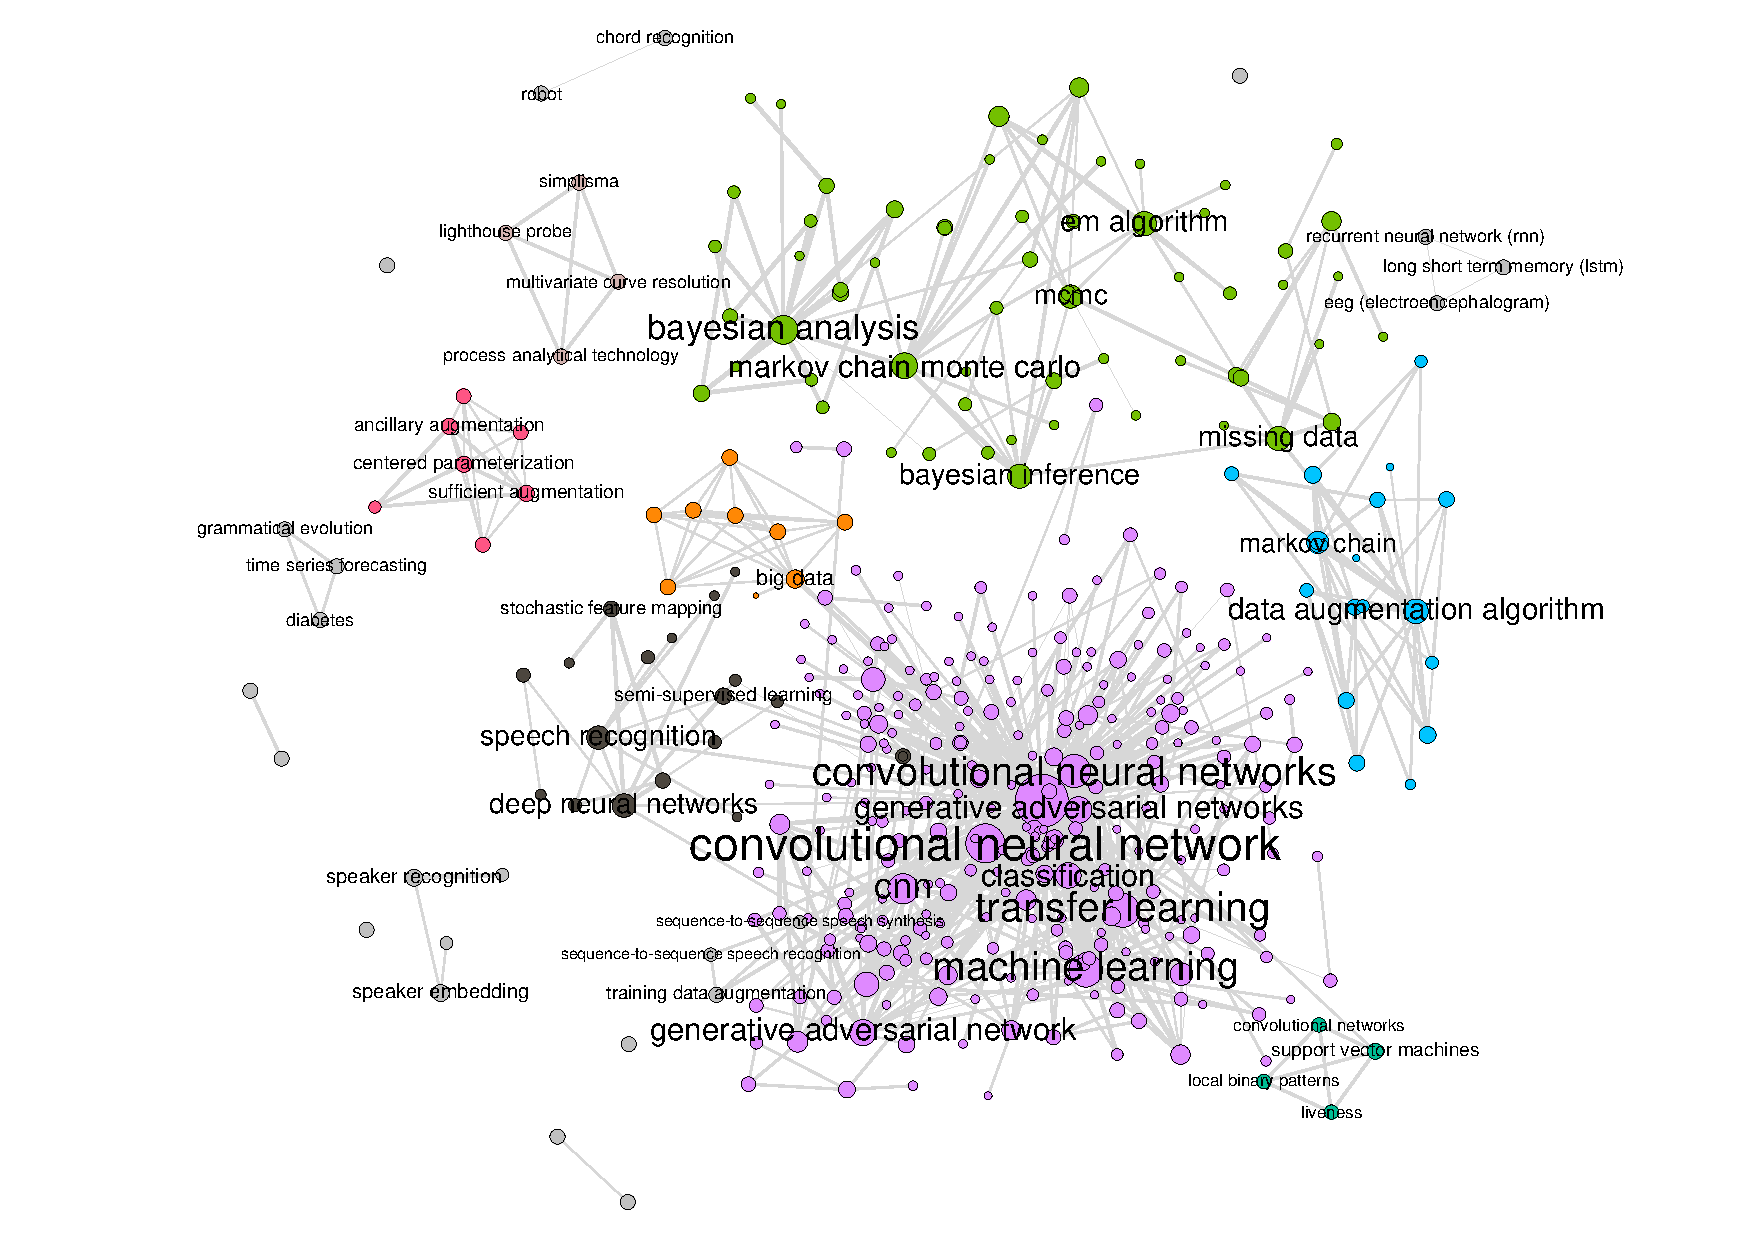
\includegraphics[width=\linewidth]{keyword_network}
    \caption{Keyword network.
    }~\label{fig:keyword_network}
\end{figure}

\subsection{Topic Analysis}

The LDA topic extraction resulted in 8 different topics, whose distribution of
topics is shown in Figure~\ref{fig:lda_topics_sankey}. The main topics within
which most articles were included is topic 5, which is defined by the main
theoretical keywords related to image data augmentation. Rather, the secondary
topic is more useful for this analysis. It is found based on the topic
likelihood of each document, excluding the dominant topic. Documents belonging
to the same group across primary, secondary and/or tertiary topics had a
likelihood of zero of belonging to any other topic.

\begin{figure}[ht]
	\centering
    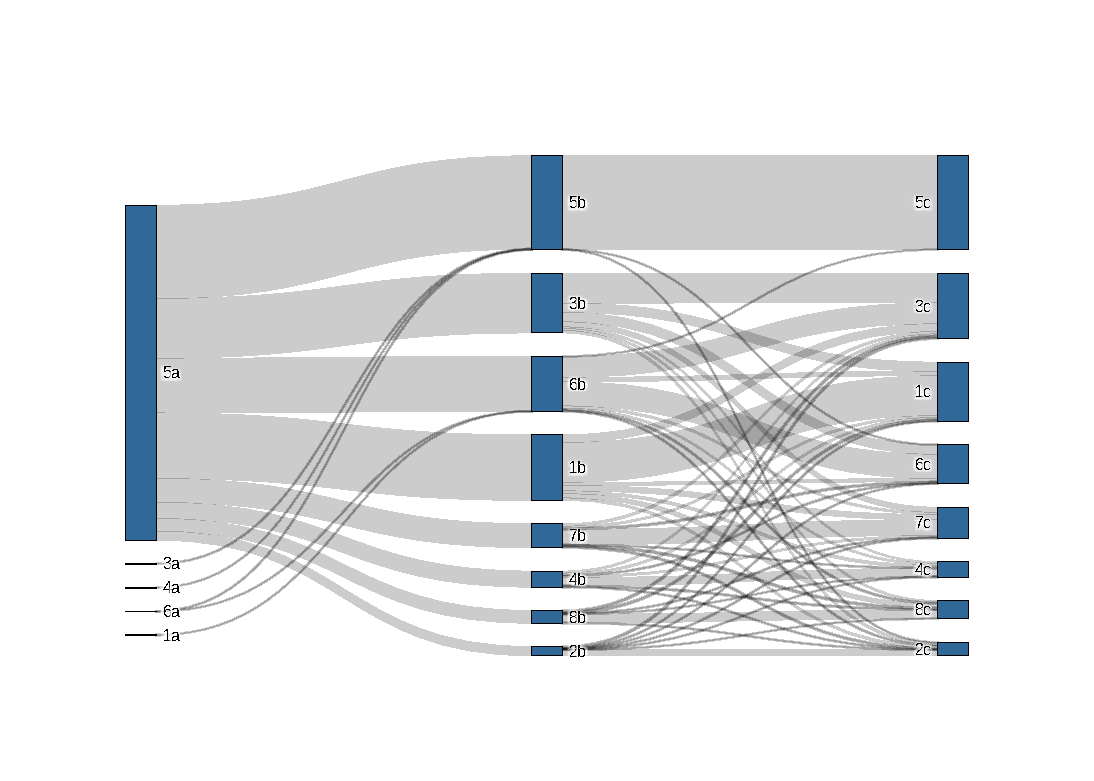
\includegraphics[width=\linewidth]{lda_topics_sankey}
    \caption[Distribution of documents over the different topics
    found.]{%
        Distribution of documents over the different topics found. The
        left column represent the primary topics, the middle column represents
        the secondary topics and the right columns represents the tertiary
        topics.
    }~\label{fig:lda_topics_sankey}
\end{figure}

The topics found in the bibliometric data are shown in
Table~\ref{tab:topic_analysis}. A few topics seem to overlap each other,
although they are generally distinguishable. The primary domains of
application of data augmentation methods differ for each different topic
identified:

\begin{enumerate}
    \item Documents in Topic 1 frequently use the word ``yolov'', which refers
        to the YOLOvX family of deep learning object detection
        models~\cite{Redmon2015}, where X refers to the version of the model
        used (the most recent version is 5). Another relevant keyword is
        ``style\_transfer'', which refers to a specific technique of data
        augmentation. 

        This topic has two primary domains of application. The keywords
        ``pest'' and ``coffe'' refer to data augmentation on agriculture
        research. The keywords ``biomed'', ``histolog'' and ``nodul'' refer to
        biomedical applications such as pulmonary nodule detection and
        histology image classification. Within these topics, a few
        domain-specific data augmentation algorithms were proposed. For
        example, in~\cite{Cicalese2020} the authors propose a style-transfer
        data augmentation method for histology image classification.  

    \item Documents in Topic 2 are primarily associated to the study of
        applications that include image data augmentation. The dominant
        keyword, ``hyperspectr\_imag'', refers to the application of data
        augmentation on hyperspectral images, commonly used in remote sensing
        and medicine. Other classification tasks include license plate
        detection (``licens\_plate''), inpainting (``inpaint''), background
        subtraction (``illumin\_chang'') and cloud shadow
        detection/segmentation (``shadow'').
    
    \item Documents in topic 3 refer to the application of data augmentation
        to deal with censored data (a condition in which the value of an
        observation is only partially known) and/or supervised tasks on data
        structured as graphs. Other domains of application involve chest
        x-rays classification (``cxr''), epidemiology (``risk\_factor'') and
        few audio/music information retrieval (``sourc\_separ'') articles.

    \item Documents in topic 4 refer to the application of data augmentation
        methods on object detection tasks. Specifically fire and smoke,
        pedestrians and crowd counting. Other applications within this topic
        are focused on speech recognition and angiography
        segmentation/classification.

    \item Documents in topic 5 are focused on image segmentation
        and classification methods where data augmentation algorithms are
        involved. It includes common keywords present in a large set of
        articles. These articles are mainly focused on the development of
        different convolutional neural network architectures (``cnn'') and
        neural network-based data augmentation methods.

    \item Documents in topic 6 are focused on Bayesian-based algorithms and
        Markov Chain algorithms. This topic includes data augmentation on
        regression tasks and misclassification detection.

    \item Documents in topic 7 covers the application of data augmentation
        into various domains. Specifically, music information retrieval
        (``music''), fish/marine organisms recognition, gender bias, speech
        recognition, random erasing 

    \item Documents in topic 8 contains remote sensing and biomedicine as the
        primary research domains. The keywords ``drone'' and ``aircraft''
        refer to the sources of data collected for remote sensing work,
        whereas ``pneumonia'' and ``chest\_rai\_imag'' refers to biomedicine
        research topics/image data.
\end{enumerate}


\begin{table}
    \begin{center}
    \begin{tabular*}{\textwidth}{@{\extracolsep{\fill}}lllllll@{\extracolsep{\fill}}}
        \toprule
        Topic & Representative Paper & Papers & Words\\
        \midrule
        1 & GAN-based synthetic medical image & 440 & yolov, pest, style\_transfer, \\
          & augmentation for increased CNN && coffe, thermal, biomed, \\
          & performance in liver lesion && scene\_text, histolog, nodul, \\
        \vspace{.2cm}& classification && visibl \\
        
        2 & CVAE-GAN: Fine-Grained Image & 61 & hyperspectr\_imag, licens\_plate, \\
          & Generation through Asymmetric && command, inpaint, \\
          & Training && illumin\_chang, upper, restor, \\
        \vspace{.2cm}  &&& ann, foreign, shadow \\
        
        3 & A survey on Image Data & 401 & censor, markov\_chain, node, \\ 
          & Augmentation for Deep Learning && team, tree, cxr, risk\_factor, \\
        \vspace{.2cm}  &&&mass, largest, sourc\_separ\\
        
        4 & Return of the devil in the details: & 108 & smoke, pedestrian, transcrib, \\
          & Delving deep into convolutional nets && crowd, children\_speech, intent, \\
          &&&adult, auxiliari\_variabl, speech, \\
        \vspace{.2cm}  &&&angiographi \\
        
        5 & U-net: Convolutional networks for & 632 & imag, detect, gener, dataset, \\
          & biomedical image segmentation && classif, sampl, network, cnn, \\
        \vspace{.2cm}  &&&featur, augment\\
        
        6 & Deep Convolutional Neural Networks & 370 & tea, multivari, \\
          & and Data Augmentation for && markov\_chain\_mont\_carlo, \\
          & Environmental Sound Classification && bayesian, regress, misclassif, \\
        \vspace{.2cm}  &&& procedur, famili, illustr, mcmc \\
        
        7 & Weakly Supervised Deep Detection & 160 & music, fish, marin, gender, \\
          & Networks && vocal, random\_eras, low\_qualiti, \\
        \vspace{.2cm}  &&& crowd, prune, bengali \\
        
        8 & An Efficient Deep Learning Approach & 85 & drone, gait, aircraft, \\      
          & to Pneumonia Classification in && gestur\_recognit, pneumonia, \\
          & Healthcare && chest\_rai\_imag, covid, walk, \\
          &&& onset, hidden\_layer \\
        \bottomrule
    \end{tabular*}
    \caption{%
        Description of the main topics found in the literature.
    }~\label{tab:topic_analysis}
    \end{center}
\end{table}

The per-year popularity of the different topics is shown in
Figure~\ref{fig:topics_per_year}. Since 2015, topic 5 gained more research
momentum, whereas topic 6 lost much of its relative popularity within the
field. In the past 5 years topics 8 and 3 have become steady research streams
while topic 1 saw a significant growth in popularity. 

\begin{figure}
	\centering
    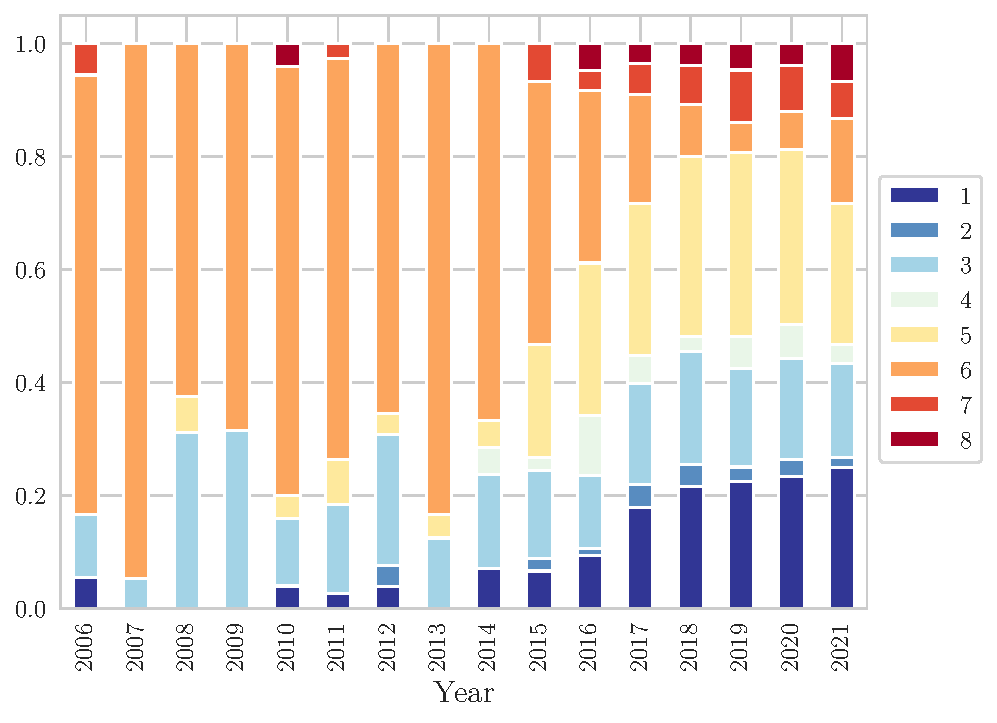
\includegraphics[width=.8\linewidth]{topics_per_year}
    \caption{Topic frequency per year.
    }~\label{fig:topics_per_year}
\end{figure}

\subsection{Research Gap Discussion}

Data augmentation mechanisms are often used as regularization methods for
deep learning classifiers. The study of data augmentation mechanisms in
ensembles of simple classifiers have achieved state-of-the-art performance not
only 10 years ago~\cite{Meier2011, Ciresan2011}, but also when compared to
modern deep learning architectures~\cite{Tolstikhin2021, Touvron2021,
Liu2021}. However, the implementation of different data augmentation methods
shows a promising path to improve the performance of simple classifiers
(and/or recent ensemble architectures) and requires further research.

A research application that was not frequently found in the literature was
small dataset augmentation. This is particularly useful for any complex
problem when the amount of labeled data available to use as training data is
scarce, which limits the usage of classification algorithms and especially
deep learning algorithms. In this context, techniques such as Active Learning
can be used to annotate a small amount of data, while maximizing the
classification performance~\cite{Su2020}. However, classifiers may not be
capable of generalizing with small training datasets and the ability to
reproduce and augment the labelled data available can further reduce
annotation cost and allow the usage of data intensive classifiers.

Another limitation found in the literature relates to the problem of
initialization on network-based data augmentation methods. The same data
augmentation algorithm trained with different initialization settings
(different random seed or training subset) may lead to different model
parameters and quality of the trained classifier.

The rapid development of data augmentation algorithms raises additional open
questions on how the data used and store for model training. Specifically, the
lower data storage and processing power available to the general public
(\textit{i.e.}, organizations and individuals) is a limitation for producing
state-of-the-art classifiers. Another problem arises from data privacy
concerns, since the usage of user data to train machine learning models
typically involve the storage of such information. However, if data
augmentation algorithms were continuously updated and capable of producing
reliable data on an as-needed basis, not only would storage requirements
decrease, but it would also become possible to work with fully artificial
data, without the need to store as much data. This would also facilitate the
sharing of datasets (in the form of an algorithm) without compromising
sensitive data.

\section{Conclusion}~\label{sec:conclusion-aug}

Depending on the domain of application, data augmentation research differs in
the format of publication. On the one hand, domains like Statistics, Remote
Sensing and Medical Imaging seem more active on journal publications,
typically in journals with high impact factor. On the other hand, research
developed in the domains of computer vision, speech recognition, acoustic
modelling, natural language processing and signal processing seem to attribute
higher importance to conference papers. Many of the influential papers we found
were focused on deep learning methods for classification, segmentation, sound
and speech recognition and remote sensing.

We analysed the different communities of keywords formed using document
keywords, as well as topic analysis using a LDA analysis over the document's
abstracts. We found various distinctive areas of research, both regarding the
data augmentation methods used and the domain of application. We found that in
recent years research on augmentation methods using Bayesian-based algorithms,
as well as Markov Chain algorithms reduced its popularity, whereas data
augmentation methods based on neural networks and deep learning classifiers
have increased its popularity.

Data augmentation is most commonly applied/studied in the realm of computer
vision for tasks like image classification, segmentation, object detection,
inpainting and background subtraction tasks, even though it may be applied to
many other data structures. It is frequently used in studies within the
domains of biomedicine, agriculture, speech recognition, acoustic modelling,
remote sensing and computational creativity. It is also used alongside other
data preprocessing techniques, such as feature extraction and dimensionality
reduction.

Although data augmentation is a vibrant area of research, there are still
significant gaps to be addressed. Data augmentation methods are increasingly
used as regularization methods for deep learning. Although, recent research
shows that the same can be done for simpler classifier configurations in order
to achieve a classification performance comparable to that of state-of-the-art
deep learning, which require further confirmation, as well as the development
of less computational intensive data augmentation methods. Other less popular
topics, such as small data augmentation, appear to have a relevant practical
importance and require further research. In addition, other limitations of
data augmentation algorithms should be addressed. One problem commonly found
in the literature is the impact the weights initialization and training set
used have in the quality of the trained algorithm. In the future, using data
augmentation methods as a source of artificial datasets can address a variety
of concerns, such as data privacy, sharing and storage. Finally, exploring
data augmentation algorithms to complement or replace techniques such as
Active Learning may reduce the cost of data collection, although it is yet to
be explored.

\thesischapter{%
    Tabular and Latent Space Synthetic Data Generation: A Literature Review
}{%
    Submitted as Joao Fonseca, Fernando Bacao, to a Q1 Journal, 2022
}~\label{chp:synthetic-data-review}
\graphicspath{{figures/synthetic-data-review/}}

\begin{adjustwidth}{30pt}{30pt}

    The generation of synthetic data can be used for anonymization,
    regularization, oversampling, semi-supervised learning, self-supervised
    learning and various other tasks. Such broad potential motivated the
    development of new algorithms, specialized in data generation for specific
    data formats and Machine Learning (ML) tasks. However, one of the most
    common data formats used in industry applications, tabular data, is
    generally overlooked; Literature analyses are scarce, state-of-the-art
    methods are spread across domains and ML tasks and there is little to no
    distinction among the main types of mechanism underlying synthetic data
    generation algorithms. In this paper, we analyse tabular and latent space
    synthetic data generation algorithms. Specifically, we propose a unified
    taxonomy as an extension and generalization of previous taxonomies, review
    70 generation algorithms across six ML problems, distinguish the main
    generation mechanisms identified into six categories, describe each type
    of generation mechanism, discuss metrics to evaluate the quality of
    synthetic data and provide recommendations for future research. We expect
    this study to assist researchers and practitioners identify relevant gaps
    in the literature and design better and more informed practices regarding
    synthetic data.

\end{adjustwidth}

\vspace{.5cm}
\textbf{Keywords:} Synthetic Data; Data Augmentation; Oversampling;
Regularization; Privacy

\section{Introduction}\label{sec:introduction-synth}

Tabular data consists of a database structured in tabular form, composed of
columns (features) and rows (observations)~\cite{yoon2020vime}. It is one of
the most commonly used data structures within a wide range of domains.
However, ML techniques developed for tabular data can be applied to any type
of data; input data, regardless of its original format, can be mapped into a
manifold, lower-dimensional abstraction of the input data and mapped back into
its original input space~\cite{kingma2019introduction, DeVries2017}.
This abstraction is often referred to as embeddings, encodings, feature
space or latent space. In this paper, we will refer to this concept as
latent space.

Synthetic data is obtained from a generative process based on properties of
real data~\cite{assefa2020generating}. The generation of synthetic data is
essential for several objectives. For example, it is used as a form of
regularizing ML classifiers (\textit{i.e.}, data
augmentation)~\cite{wang2021regularizing}. One form of anonymizing datasets is
via the production of synthetic observations (\textit{i.e.}, synthetic data
generation)~\cite{patki2016synthetic}. In settings where only a small portion
of training data is labeled, some techniques generate artificial data using
both labeled and unlabeled data with a modified loss function to train neural
networks (\textit{i.e.}, semi-supervised learning)~\cite{laine2017temporal}.
In imbalanced learning contexts, synthetic data can be used to balance the
target classes' frequencies and reinforce the learning of minority classes
(\textit{i.e.}, oversampling)~\cite{Fonseca2021}. Some active
learning frameworks use synthetic data to improve data selection and
classifier training~\cite{Kim2021}. Other techniques employ data
generation to train neural networks without labeled data (\textit{i.e.},
self-supervised learning)~\cite{grill2020bootstrap}.

The breadth of these techniques span multiple domains, such as facial
recognition~\cite{lv2017data}, Land Use/Land Cover
mapping~\cite{Douzas2019rs}, medical image
processing~\cite{yi2019generative}, Natural Language Processing
(NLP)~\cite{feng2021survey} or credit card default
prediction~\cite{alam2020investigation}. According to the domain and data
type, the data generation techniques used may vary significantly. In addition,
several synthetic data generation methods are specific to the domain, data
type or target ML task. Generally, these methods rely on the domain data's
structure, which are not easily transferable to tabular data.

Overall, synthetic data generation techniques for tabular data are not as
explored as image or text data, despite its popularity and
ubiquity~\cite{fakoor2020fast}. Furthermore, these techniques are invariant to
the original data format; they can be applied to both the latent
space~\cite{DeVries2017} or tabular data. On one hand, data generation
in the latent space uses a generative model to learn a manifold,
lower-dimensional abstraction over the input
space~\cite{kingma2019introduction}. At
this level, any tabular data generation mechanism can be applied and
reconstructed into the input space if necessary. On the other hand, synthetic
data generation on tabular data can be applied to most problems. Although, the
choice of generation mechanism depends on (1) the importance of the original
statistical information and the relationships among features, (2) the target
ML task and (3) the role synthetic data plays in the process (\textit{i.e.},
anonymization, regularization, class balancing, etc.).  For example, when
generating data to address an imbalanced learning problem (\textit{i.e.},
oversampling), the relationships between the different features are not
necessarily kept, since the goal is to reinforce the learning of the minority
class by redefining an ML classifier's decision boundaries. If the goal is to
anonymize a dataset, perform some type of descriptive task, or ensure
consistent model interpretability, statistical information must be preserved.

Depending on the context, evaluating the quality of the generated data is a
complex task. For example, for image and time series data, perceptually small
changes in the original data can lead to large changes in the euclidean
distance~\cite{assefa2020generating, theis2016note}. The evaluation of
generative models typically account primarily for the performance in a
specific task, since good performance in one criterion does not imply good
performance on another~\cite{theis2016note}. However, in computationally
intensive tasks it is often impracticable to search for the optimal
configurations of generative models. To address this limitation, other
evaluation methods have been proposed to assist in this evaluation, which
typically use statistical divergence metrics, averaged distance metrics,
statistical similarity measurements, or precision/recall
metrics~\cite{chundawat2022tabsyndex, alaa2022faithful}. The relevant
performance metrics found in the literature are discussed in
Section~\ref{sec:evaluating-synthetic-data-synth}.

\subsection{Motivation, Scope and Contributions}

% TODO: Define scope
% - Exclude domain-specific traditional applications
% - Exclude Generation techniques with an internal application level
% - Preference for methods published in 2019 or later, 
%   non-traditional methods, or unique/uncommon approaches
% - To avoid redundancy, this is a non-comprehensive analysis of algorithms
%   and problems using synthetic data. Instead, we show the most important
%   methods using each of the data generation mechanisms found. For example,
%   there are several oversampling algorithms available, but most of those
%   excluded from this analysis use a linear (SMOTE-based) generation
%   mechanism.

This literature review focuses on generation mechanisms applied to tabular
data across the main ML techniques where tabular synthetic data is used.  We
also discuss generation mechanisms used in the latent space, since the
generation mechanisms in tabular data and latent space may be used
interchangeably. In addition, we focus on the ML perspective of synthetic
data, as opposed to the practical perspective; according to the practical
perspective, synthetic data is used as a proxy of real data. It is assumed to
be inaccessible, essential and a secondary asset for tasks like education,
software development, or systems demonstrations~\cite{mannino2019real}. 

We focus on data generation techniques in the tabular and latent space
(\textit{i.e.}, embedded inputs) with a focus on classification and associated
ML problems. Related literature reviews are mostly focused on specific
algorithmic or domain applications, with little to no emphasis on the core
generative process. For this reason, these techniques often appear
``sandboxed'', even though there is a significant overlap between them. There
are some related reviews published since 2019. \citet{assefa2020generating}
provides a general overview of synthetic data generation for time series data
anonymization in the finance sector. \citet{hernandez2022synthetic} reviews
data generation techniques for tabular health records anonymization.
\citet{raghunathan2021synthetic} reviews synthetic data anonymization
techniques that preserve the statistical properties of a dataset.
\citet{nalepa2019data} reviews data augmentation techniques for brain-tumor
segmentation. \citet{bayer2021survey} distinguishes augmentation techniques
for text classification into latent and data space, while providing an
extensive overview of augmentation methods within this domain. However, the
taxonomy proposed and latent space augmentation methods are not necessarily
specific to the domain. \citet{shorten2021text}, \citet{chen2021empirical},
\citet{feng2021survey} and \citet{liu2020survey} also review data augmentation
techniques for text data.  \citet{yi2019generative} review Generative
Adversarial Network architectures for medical imaging. \citet{wang2020survey}
reviews face data augmentation techniques. \citet{Shorten2019},
\citet{khosla2020enhancing} and \citet{khalifa2021comprehensive} discuss
techniques for image data augmentation.  \citet{Iwana2021} and
\citet{wen2020time} also review time series data augmentation techniques.
\citet{zhao2022graph} review data augmentation techniques for graph data. The
analysis of related literature reviews~\footnote{Results obtained using Google
    Scholar, limited to articles published since 2019, using the search query
    {\fontfamily{qcr}\selectfont (``synthetic data generation'' OR
        ``oversampling'' OR ``imbalanced learning'' OR ``data augmentation'')
        AND (``literature review'' OR ``survey'')}. Retrieved on August
    $11^{th}$, 2022. More articles were added later whenever found relevant.
} is shown in Table~\ref{tab:literature-reviews}.

% TODO: move table to appendix (?)
\begin{table}[t!]
    \centering
    \caption{\label{tab:literature-reviews}
        Related literature reviews published since 2019.
    }
    \small{%
    \begin{tabularx}{\textwidth}{@{}rcccX@{}}
        \toprule
        Reference & Data type & ML problem & Domain & Observations \\
        \midrule

        \citet{assefa2020generating} & --- & Data privacy &
        Finance & Analysis of applications, motivation and properties of
        synthetic data for anonymization. \\

        \citet{hernandez2022synthetic} & Tabular & Data privacy &
        Healthcare & Focus on GANs. \\

        \citet{raghunathan2021synthetic} & Tabular & Data privacy &
        Statistics & Focus on general definitions such as differential privacy
        and statistical disclosure control.\\

        \citet{nalepa2019data} & Image & Segmentation & Medicine & Analysis of
        algorithmic applications on a 2018 brain-tumor segmentation
        challenge.\\

        \citet{bayer2021survey} & Text & Classification & --- & Distinguish
        100 methods into 12 groups. \\

        \citet{shorten2021text} & Text & Deep Learning & --- & General
        overview of text data augmentation. \\

        \citet{chen2021empirical} & Text & Few-shot Learning & --- &
        Augmentation techniques for machine learning with limited data\\

        \citet{feng2021survey} & Text & --- & --- & Overview of augmentation
        techniques and applications on NLP tasks.\\

        \citet{liu2020survey} & Text & --- & Various & Analysis of industry
        use cases of data augmentation in NLP\@. Emphasis on input level data
        augmentation.\\

        \citet{yi2019generative} & Image & --- & Medicine & Emphasis on GANs.\\

        \citet{wang2020survey} & Image & Deep Learning & --- & Regularization
        techniques using facial image data. Emphasis on Deep Learning
        generative models.\\

        \citet{Shorten2019} & Image & Deep Learning & --- & Emphasis on
        data augmentation as a regularization technique.\\

        \citet{khosla2020enhancing} & Image & --- & --- & Broad overview of
        image data augmentation. Emphasis on traditional approaches. \\

        \citet{khalifa2021comprehensive} & Image & --- & Various & General
        overview of image data augmentation and relevant domains of
        application.\\

        \citet{Iwana2021} & Time series & Classification & --- &
        Defined a taxonomy for time series data augmentation.\\

        \citet{wen2020time} & Time series & Various & --- & Analysis of data
        augmentation methods for classification, anomaly detection and
        forecasting.\\

        \citet{zhao2022graph} & Graph & Various & --- & Graph data
        augmentation for supervised and self-supervised learning.\\

        \bottomrule
        
    \end{tabularx}
    }
\end{table}


The different taxonomies established in the literature follow a similar
philosophy, but vary in terminology and are often specific to the technique
discussed. Regardless, it is possible to establish a broader taxonomy without
giving up on specificity. This study provides a joint overview of the
different data generation approaches, domains and ML techniques where data
generation is being used, as well as a common taxonomy across domains. It
extends the analyses found in these articles and uses the compiled knowledge
to identify research gaps. We compare the strengths and weaknesses of the
models developed within each of these fields. Finally, we identify possible
future research directions to address some of the limitations found. The
contributions of this paper are summarized below:

\begin{itemize}

    \item Bridge different ML concepts using synthetic data generation in its
        core;

    \item Propose a synthetic data generation/data augmentation taxonomy to
        address the ambiguity in the various taxonomies proposed in the
        literature;

    \item Characterize all the relevant data generation methods using the
        proposed taxonomy;

    \item Discuss the ML techniques in which synthetic data generation is used
        and consolidate the current generation mechanisms across the
        different techniques;

    \item Highlight the key challenges of synthetic data generation and
        discuss possible future research directions.

\end{itemize}

\subsection{Paper Organization}

The rest of this paper is organized as follows: Section~\ref{sec:background-synth}
defines and formalizes the different concepts, goals, trade-offs and
motivations related to synthetic data generation. Section~\ref{sec:taxonomy-synth}
defines the taxonomy used to categorize all the algorithms analysed in this
study. Section~\ref{sec:algorithmic-applications-synth} analyses all the algorithms
using synthetic data generation, distinguished by learning problem.
Section~\ref{sec:generation-mechanisms-synth} describes the main generation
mechanisms found, distinguished by generation type.
Section~\ref{sec:evaluating-synthetic-data-synth} reviews performance evaluation
methods of synthetic data generation mechanisms. Section~\ref{sec:discussion-synth}
summarizes the main findings and general recommendations for good practices on
synthetic data usage. Section~\ref{sec:future-work-synth} discusses limitations,
research gaps and future research directions. Section~\ref{sec:conclusions-synth}
presents the main conclusions drawn from this study.

\section{Background}\label{sec:background-synth}

In this section we define basics concepts, common goals, trade-offs and
motivations regarding the generation of synthetic data in ML\@. We define
synthetic data generation as the production of artificial observations that
resemble naturally occurring ones within a certain domain, using a generative
model. It requires access to a training dataset, a generative process, or a
data stream. However, the constraints imposed to this process largely depends
on the target ML task. For example, to generate artificial data for
regularization purposes in supervised learning (\textit{i.e.}, data
augmentation) the training dataset must be annotated. The production of
anonymized datasets using synthetic data generation requires synthetic
datasets to be different from the original data, while following similar
statistical properties. Domain knowledge may also be necessary to encode
specific relationships among features into the generative process.


\subsection{Relevant Learning Problems}

%% Anonymize datasets (differential privacy)
The breach of sensitive information is an important barrier to the sharing of
datasets, especially when it concerns personal
information~\cite{dankar2021fake}. One solution for this problem is the
generation of synthetic data without identifiable information. Generally
speaking, ML tasks that require data with sensitive information are not
compromised when using synthetic data. The experiment conducted by
\citet{patki2016synthetic} using relational datasets showed that in 11 out 15
comparisons ($\approx 73\%$), practitioners performing predictive modelling
tasks using fully synthetic datasets performed the same or better than those
using the original dataset. Optionally, anonymized synthetic data may be
produced with theoretical privacy guarantees, using differential privacy
techniques. This topic is discussed in Section~\ref{sec:data-privacy-synth}.

%% Generalization/regularization
A common problem in the training of deep neural networks are their capacity to
generalize~\cite{Zhang2021} (\textit{i.e.}, reduce the difference in
classification performance between known and unseen observations). Data
augmentation is a common method to address this problem for any type of ML
classifier. The generation of synthetic observations increases the range of
the input space used in the training phase and reduces the difference in
performance between known and new observations. Although other regularization
methods exist, data augmentation is a useful method since it does not affect
the choice in the architecture of the ML classifier and does not exclude the
usage of other regularization methods. In domains such as computer vision and
NLP, data augmentation is also used to improve the robustness of models
against adversarial attacks~\cite{zeng2020data, morris2020textattack}. These
topics are discussed into higher detail in Section~\ref{sec:regularization-synth}.

%% Oversampling
In supervised learning, synthetic data generation is often motivated by the
need to balance target class distributions (\textit{i.e.}, oversampling).
Since most ML classifiers are designed to perform best with balanced datasets,
defining an appropriate decision boundary to distinguish rare classes becomes
difficult~\cite{saez2016analyzing}. Although there are other approaches to
address imbalanced learning, oversampling techniques are generally easier to
implement since they do not involve modifications to the classifier. This
topic is discussed into higher detail in Section~\ref{sec:oversampling-synth}.

%% Active Learning + Few-shot Learning
In supervised learning tasks where labeled data is not readily available, but
can be labeled, an Active Learning (AL) method may be used to improve the
efficiency of the labelling process. AL aims to reduce the cost of producing
training datasets by finding the most informative observations to label and
feed into the classifier~\cite{Fonseca2021al}. In this case, the
generation of synthetic data is particularly useful to reduce the amount of
labelled data required for a successful ML project. This topic is discussed in
Section~\ref{sec:active-learning-synth}.

%% Semi-supervised Learning + Self-supervised learning
Two other techniques reliant on synthetic data generation are Semi-supervised
Learning (Semi-SL) and Self-Supervised Learning (Self-SL). The former
leverages both labeled and unlabeled data in the training phase,
simultaneously, while several methods apply perturbations on the training data
as part of the training procedure~\cite{Van2020}. The latter, Self-SL,
is a technique used to train neural networks in the absence of labeled data.
Several Semi-SL and Self-SL methods use synthetic data generation as a core
element. These methods are discussed in
Sections~\ref{sec:semi-supervised-learning-synth}
and~\ref{sec:self-supervised-learning-synth}.


% Concepts definition, goals + trade-offs, Motivations

% Concepts definition
% - Original dataset
% - Synthetic dataset
% - Generator
% - Quality criteria (e.g., similarity function)
% - Objective performance metric (ML method to improve)
 
% Common success criteria 
% - The synthetic dataset should be different than the original dataset (i.e.,
%   no duplicates)
% - It should minimize a similarity function
% - The statistical properties of the dataset are preserved
% - It should improve the output of the objective performance
 
% Trade-offs
% - Additional computational overhead
% - Expose the classifier to unfeasible input areas

\subsection{Problem Formulation}\label{sec:problem-formulation-synth}

The original dataset, $\mathcal{D} = \mathcal{D}_L \cup \mathcal{D}_U$,
is a collection of real observations and is distinguished according to whether
a target feature exists, $\mathcal{D}_L = {((x_i, y_i))}^l_{i=1}$, or not,
$\mathcal{D}_U = {(x_i)}^{u}_{i=1}$. All three datasets, $\mathcal{D}$,
$\mathcal{D}_L$ and $\mathcal{D}_U$ consist of ordered collections with
lengths $l+u$, $l$ and $u$, respectively. Synthetic data generation is
performed using a generator, $f_{gen}(x;\tau) = x^s$, where $\tau$
defines the generation policy (\textit{i.e.}, its hyperparameters), $x \in
\mathcal{D}$ is an observation and $x^s \in \mathcal{D}^s$ is a
synthetic observation. Analogous to $\mathcal{D}$, the synthetic dataset,
$\mathcal{D}^s$, is also distinguished according to whether there is an
assignment of a target feature, $\mathcal{D}^s_L = {((x^s_j,
y^s_j))}^{l'}_{j=1}$, or not, $\mathcal{D}^s_U =
{(x^s_j)}^{u'}_{j=1}$.

% - Quality criteria (e.g., similarity function)
Depending on the ML task, it may be relevant to establish metrics to measure
the quality of $\mathcal{D}^s$. In this case, a metric
$f_{qual}(\mathcal{D}^s, \mathcal{D})$ is used to determine the level of
similarity/dissimilarity between $\mathcal{D}$ and $\mathcal{D}^s$. In
addition, a performance metric to estimate the performance of a model on the
objective task, $f_{per}$, may be used to determine the appropriateness of a
model with parameters $\theta$, \textit{i.e.}, $f_{\theta}$. The generator's
goal is to generate $\mathcal{D}^s$ with arbitrary length, given
$\mathcal{D} \sim \mathbb{P}$ and $\mathcal{D}^s \sim \mathbb{P}^s$, such
that $\mathbb{P}^s \approx \mathbb{P}$, $x_i \neq x_j \forall x_i \in
\mathcal{D} \wedge x_j \in \mathcal{D}^s$. $f_{gen}(x;\tau)$ attempts to
generate a $\mathcal{D}^s$ that maximizes either $f_{per}$, $f_{qual}$, or a
combination of both.


\section{Data Generation Taxonomy}\label{sec:taxonomy-synth}

The taxonomy proposed in this paper is a combination of
different definitions found in the literature, extended with other traits that
vary among domains and generation techniques. Within image data studies,
\citet{Shorten2019} and \citet{khalifa2021comprehensive} divide data
augmentation techniques into ``basic'' or ``classical'' approaches and deep
learning approaches. In both cases, the former refers to domain-specific
generation techniques, while the latter may be applied to any data structure.
\citet{Iwana2021} proposes a time-series data augmentation taxonomy
divided in four families: (1) Random transformation, (2) Pattern mixing, (3)
Generative models and (4) Decomposition. With exception to generative models,
the majority of the methods presented in the remaining families are well
established and domain specific. \citet{hernandez2022synthetic} defines a
taxonomy for synthetic tabular data generation approaches divided in three
types of approaches: (1) Classical, (2) Deep learning and (3) Others. Most
taxonomies follow similar definitions, while varying in terminology
or distinction criteria. In addition, all taxonomies with categories defined
as ``basic'', ``traditional'' or ``classical'' use these to characterize
domain-specific transformations.

Within the taxonomies found, none of them consider how a generation
mechanism employs $\mathcal{D}$ into the generation process or, if
applicable, the training phase. However, it is important to understand whether
a generation mechanism randomly selects $x$ and a set of close neighbors, thus
considering local information only, or considers the overall dataset or data
distribution for the selection of $x$ and/or generation of $x^s$. Our
proposed taxonomy is depicted in Figure~\ref{fig:data-generation-taxonomy}. It
characterizes data generation mechanisms using four properties:

\begin{enumerate}

    \item Architecture. Defines the broader type of data augmentation. It is
        based on domain specificity, architecture type or data transformations
        using a heuristic or random perturbation process. Data generation
        based on data sampling from a probability function is considered
        probability-based. Generation techniques that apply a form of random
        perturbation, interpolation or geometric transformation to the data
        with some degree of randomness are considered randomized approaches.
        Typical, domain-specific data generation techniques are considered
        domain-specific approaches. These techniques apply transformations to
        a data point leveraging relationships in the structure of the data
        (which is known \textit{a priori}). Generative models based on neural
        network architectures are defined as network-based. These
        architectures attempt to either generate observations in the latent
        space and/or by producing observations that are difficult to
        distinguish from the original dataset.

    \item Application level. Refers to the phase of the ML pipeline where the
        generative process is included. Generative models are considered
        internal if they are used alongside the primary ML task, whereas
        models used prior to the development of the primary ML task are
        considered external.

    \item Scope. Considers the usage of the original dataset's properties.
        Generative models that consider the density of the data space,
        statistical properties of $\mathcal{D}$, or attempt to
        replicate/manipulate specific relationships found in $\mathcal{D}$ are
        considered to have a global scope, whereas generative models that
        consider a single observation and/or a set of close neighbors are
        considered to have a local scope. On the one hand, generative models
        with a local scope do not account for $\mathbb{P}^s$ but allow for the
        generation of $x^s$ within more precise regions in the
        latent/input space. On the other hand, generative models with a
        global scope have a higher capacity to model $\mathbb{P}^s$ but
        produce $x^s$ with less precision within the latent/input
        space.

    \item Data space. Refers to the type of data representation used to apply
        the generative model. Generation mechanisms can be applied using the
        raw dataset (\textit{i.e.}, on the input space), an embedded
        representation of the data (\textit{i.e.}, on the latent space) or
        based on the target feature (\textit{i.e.}, on the output space).
        Although some studies discuss the need to generate synthetic data on
        the input space~\cite{dankar2021fake, patki2016synthetic}, there are
        various studies that successfully apply synthetic data generation
        techniques on a latent space.

\end{enumerate}

\begin{figure}
	\centering
	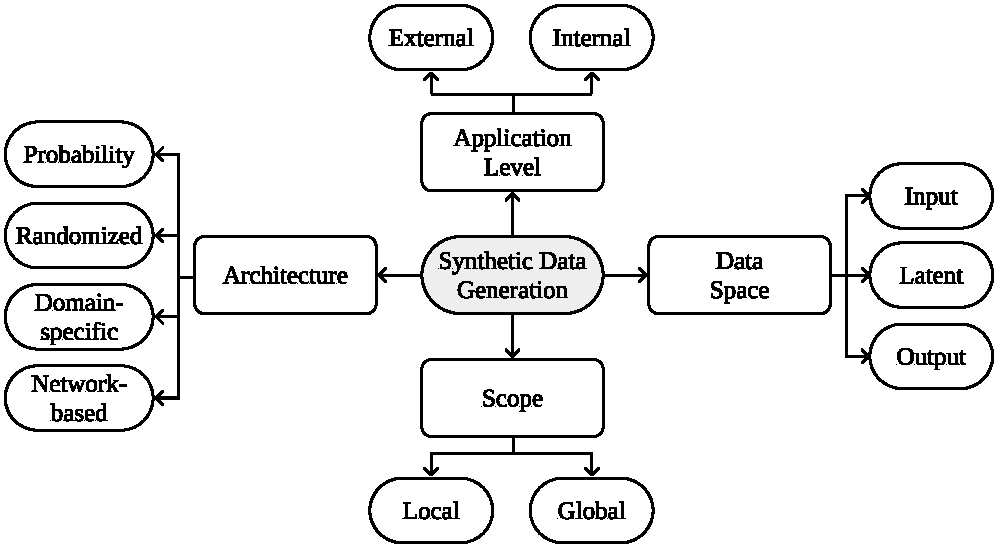
\includegraphics[width=.8\linewidth]{data-generation-taxonomy}
    \caption{General taxonomy of data generation mechanisms proposed in this
        paper.
    }~\label{fig:data-generation-taxonomy}
\end{figure}

Throughout the analysis of the different types of generation mechanisms, all
relevant methods were characterized using this taxonomy and listed in
Table~\ref{tbl:generators-synth}.

\begingroup\small
\begin{longtable}{rcccccccc}
    \caption{Summary of the synthetic data generation methods discussed in this work.}
    \label{tbl:generators-synth}\\
    \toprule
               Algorithm & ML Problem & Type &  Architecture & Level &  Data
               Space & Scope \\
    \midrule
    \endfirsthead
    \caption[]{Summary of the synthetic data generation methods discussed in this work.} \\
    \toprule
               Algorithm & ML Problem & Type &  Architecture & Level &  Data
               Space & Scope \\
    \midrule
    \endhead
    \midrule
    \multicolumn{9}{r}{{Continued on next page}} \\
    \midrule
    \endfoot
    
    \bottomrule
    \endlastfoot
    SDV~\cite{patki2016synthetic} & Anon. & PDF & Probabilistic & External & Input & Global \\
    MST~\cite{mckenna2021winning} & DP & PGM & Probabilistic & External & Input & Global \\
    MWEM~\cite{hardt2012simple} & DP & Other & Probabilistic & External & Input & Global \\
    MWEM-PGM~\cite{mckenna2019graphical} & DP & PGM & Probabilistic & External & Input & Global \\
    PrivBayes~\cite{zhang2017privbayes} & DP & PGM & Probabilistic & External & Input & Global \\
    DPGAN~\cite{xie2018differentially} & DP & GAN & Network & External & Latent & Global \\
    DPCTGAN~\cite{rosenblatt2020differentially} & DP & GAN &  Network & External & Latent & Global \\
    PATE-GAN~\cite{jordon2018pate} & DP & GAN & Network & External & Lat. + Out. & Global \\
    PATECTGAN~\cite{rosenblatt2020differentially} & DP & GAN & Network & External & Lat. + Out. & Global \\
    FEM~\cite{vietri2020new} & DP & Perturb. & Probabilistic & External & Input & Global \\
    RAP~\cite{aydore2021differentially} & DP & Perturb. & Probabilistic & External & Input & Global \\
    PDF~\cite{de2019formal, suciu2011probabilistic} & --- & PDF & Probabilistic & External & Input & Global \\
    Kamino~\cite{ge2021kamino} & DP & PDF & Probabilistic & External & Input & Global \\
    RON-GAUSS~\cite{chanyaswad2019ron} & DP & PDF & Probabilistic & Internal & Latent & Global \\
    HDMM~\cite{mckenna2018optimizing} & DP & Perturb. & Probabilistic & External & Input & Global \\
    DualQuery~\cite{gaboardi2014dual} & DP & Other & Probabilistic & External & Input & Global \\
    ROS(E)~\cite{menardi2014training} & Ovs & Perturb. & Randomized & External & Input & Local \\ 
    SMOTE~\cite{Chawla2002} & Ovs & Linear & Randomized & External & Input & Local \\
    SMOTENC~\cite{Chawla2002} & Ovs & Linear & Randomized & External & Input & Local \\
    SMOTEN~\cite{Chawla2002} & Ovs & --- & --- & External & Input & Local \\
    Borderline-SMOTE~\cite{Han2005} & Ovs & Linear & Randomized & External & Input & Local \\
    G-SMOTE~\cite{Douzas2019} & Ovs & Geometric & Randomized & External & Input & Local \\
    ADASYN~\cite{HaiboHe2008} & Ovs & Linear & Randomized & External & Input & Local \\
    KernelADASYN~\cite{tang2015kerneladasyn} & Ovs & PDF & Probabilistic & External & Input & Local \\
    MOKAS~\cite{lin2017minority} & Ovs & Other & Network & External & Latent & Global \\
    SOMO~\cite{Douzas2017} & Ovs & Linear & Net.+Rand. & External & Input & Global \\
    G-SOMO~\cite{douzas2021g} & Ovs & Geometric & Net.+Rand. & External & Input & Global \\
    GMM-SENN~\cite{xing2022predict} & Ovs & PDF & Probabilistic & External & Input & Global \\
    GMF-SMOTE~\cite{xu2022synthetic} & Ovs & Linear & Randomized & External & Input & Global \\
    C-VAE~\cite{dai2019generative} & Ovs & AE & Network & External & Latent & Global \\
    Safe-level SMOTE~\cite{bunkhumpornpat2009safe} & Ovs & Linear & Randomized & External & Input & Local \\
    LR-SMOTE~\cite{liang2020lr} & Ovs & Linear & Randomized & External & Input & Global \\
    K-means SMOTE~\cite{Douzas2018} & Ovs & Linear & Randomized & External & Input & Global\\
    DBSMOTE~\cite{bunkhumpornpat2012dbsmote} & Ovs & Linear & Randomized & External & Input & Local\\
    CGAN~\cite{douzas2018effective} & Ovs & GAN & Network & External & Latent & Global \\
    K-means CTGAN~\cite{an2021k} & Ovs & GAN & Network & External & Latent & Global \\
    SMOTER~\cite{torgo2013smote} & Ovs + Reg & Linear & Randomized & External & Input & Local \\
    G-SMOTER~\cite{camacho2022geometric} & Ovs + Reg & Linear & Randomized & External & Input & Local \\
    RACOG~\cite{das2014racog} & Ovs & PGM & Probabilistic & External & Input & Global \\
    wRACOG~\cite{das2014racog} & Ovs & PGM & Probabilistic & External & Input & Global \\
    RWO~\cite{zhang2014rwo} & Ovs & PGM & Probabilistic & External & Input & Global \\
    PDFOS~\cite{gao2014pdfos} & Ovs & PDF & Probabilistic & External & Input & Global \\
    Mixup~\cite{zhang2018mixup} & DA & Linear & Randomized & External & In.+Out. & Local \\
    M-Mixup~\cite{verma2019manifold} & DA & Linear & Network & Internal & Lat.+Out. & Global \\
    NL-Mixup~\cite{guo2020nonlinear} & DA & Geometric & Randomized & External & In.+Out. & Local \\
    AE-DA~\cite{feng2020autuencoder} & DA & AE & Network & External & In./Lat.+Out. & Local \\
    MODALS~\cite{cheung2020modals} & DA & --- & Network & Internal & Latent & Global \\
    LSI~\cite{liu2018data} & DA & AE & Network & External & Lat.+Out. & Global \\
    Gibbs~\cite{fakoor2020fast} & DA & PGM & Probabilistic & External & Input & Global \\
    MedGAN~\cite{armanious2020medgan} & DA & GAN & Network & External & Latent & Global \\
    GANBLR~\cite{zhang2021ganblr} & DA & PGM & Probabilistic & External & Input & Global \\
    Table-GAN~\cite{park2018data} & DA & GAN & Network & External & Latent & Global \\
    CTGAN~\cite{xu2019modeling} & DA & GAN & Network & External & Latent & Global \\
    TVAE~\cite{xu2019modeling} & DA & AE & Network & External & Latent & Global \\
    AE~\cite{delgado2021deep} & DA & AE & Network & External & Latent & Global \\
    InfoMixup~\cite{Kim2021} & AL & Linear & Network & Internal & Lat.+Out. & Global \\
    VAEACGAN~\cite{tran2019bayesian} & AL & AE & Network & Internal & Latent & Global\\
    AL-G-SMOTE~\cite{Fonseca2021al} & AL & Geometric & Randomized & Internal & Input & Local\\
    DAE~\cite{rasmus2015semi} & Semi-SL & AE & Network & Internal & Input & Global \\ 
    $\Pi$-model~\cite{samuli2017temporal} & Semi-SL & Perturb. & Randomized & Internal & In.+Lat. & Local \\
    Mean Teacher~\cite{tarvainen2017mean} & Semi-SL & Perturb. & Randomized & Internal & In.+Lat. & Local \\
    ICT~\cite{verma2022interpolation} & Semi-SL & Linear & Randomized & Internal & Input & Local \\
    Mixmatch~\cite{berthelot2019mixmatch} & Semi-SL & Linear & Randomized & Internal & Input & Local \\
    SDAT~\cite{fang2022semi} & Semi-SL & AE+PDF & Net.+Prob. & Internal & Latent & Global \\
    MCoM~\cite{li2022mcom} & Semi-SL & Linear & Randomized & Int.+Ext. & Inp.+Lat. & Global \\
    C-Mixup~\cite{darabi2021contrastive} & Semi/Self-SL & AE+Lin. & Net+Rand.  & Internal & Latent & Global \\
    VIME~\cite{yoon2020vime} & Semi/Self-SL & Perturb. & Randomized & Internal & Input & Local \\
    SubTab~\cite{ucar2021subtab} & Self-SL & Perturb. & Rand.+Prob. & Internal & Input & Local \\
    Scarf~\cite{bahri2022scarf} & Self-SL & Perturb. & Randomized & Internal & Input & Local \\
    A-SFS~\cite{qiu2022sfs} & Self-SL & Perturb. & Randomized & Internal & Input & Local \\
\end{longtable}
\endgroup


% \section{Data Generation in the Input Space}~\label{sec:input-space-synth}
% 
% In this section, we describe some popular domain and data type-specific data
% generation techniques. For each data type we include a table with related
% literature reviews specific to different domains.
% 
% \subsection{Supervised data generation}
% % TODO: 
% % - Table with literature review references 
% 
% \subsection{Unsupervised data generation}
% % TODO: 
% % - Table with literature review references 

% \subsection{Image}
% % TODO: 
% % - Table with literature review references 
% 
% Image-specific data generation mechanisms can be further divided into
% traditional and semantic techniques~\cite{wang2021regularizing}. Traditional
% generation techniques comprise simple modifications such as translation,
% cropping or random erasing~\cite{zhong2017random}. Semantic generation methods
% involve more complex tasks, such changing colors of specific attributes,
% backgrounds and visual angles \textbf{[CITATION]}. 
% % Go back to explaining wang2021regularizing
% 
% % semantic generation technique
% Data generation by modifying specific attributes in data points with known
% perturbations~\cite{lv2017data}. For example, overlaying facial elements into
% a picture containing a human face (\textit{e.g.}, adding sunglasses and
% different hairstyles), introducing perturbations in facial landmarks,
% different illumination and artificial misalignment are different approaches to
% generate artificial observations for facial recognition.
% 
% % GANs
% Generative Adversarial Networks in computer vision~\cite{wang2021generative}

% traditional
% - mixup

% \subsection{Text}
% % TODO: 
% % - Table with literature review references 
% 
% NLP motivations~\cite{feng2021survey}:
% 
% \begin{enumerate}
%     \item Low-resource languages (NLP)
%     \item Mitigate bias
%     \item Fixing class imbalance
%     \item Few-shot learning
%     \item Adversarial examples
% \end{enumerate}
% 
% 
% NLP also benefit from data augmentation~\cite{feng2021survey}.
% 
% In NLP, there is the challenge of establishing universal rules for text
% transformations to provide new linguistic patterns~\cite{bayer2022data}
% 
% https://github.com/styfeng/DataAug4NLP
% 
% \subsection{Graphs}
% 
% 
% Another relevant paper~\cite{zhou2020data}
% 
% Various graph data augmentation methods can be applied to related data types
% such as text data~\cite{shorten2021text}.
% 
% 
% An analysis on different graph data augmentation techniques and a new graph
% data augmentation framework~\citet{zhao2021data}
% 
% List of papers about graph data augmentation:
% https://github.com/zhao-tong/graph-data-augmentation-papers




% \section{Data Generation in the Feature Space}~\label{sec:feature-space-synth}
% % Feature level data augmentation
% 
% The concept of data generation in the feature space was popularized
% with~\cite{devries2017dataset}.
% 
% According to~\cite{assefa2020generating}. The generation of synthetic data
% should aim to fulfil the conditions below:
% 
% \begin{itemize}
%     \item Privacy preserving.
%     \item Human readable.
%     \item Compact.
% \end{itemize}
% 
% Discuss Auto-augmentation (as mentioned in~\cite{wang2020survey}) or meta
% learning (as mentioned in~\cite{Shorten2019})

\section{Algorithmic applications}\label{sec:algorithmic-applications-synth}

In this section we discuss the data generation mechanisms for the different
contexts where they are applied. We emphasize the constraints in each problem
that condition the way generation mechanisms are used. The literature search
was conducted with the Google Scholar database, using multiple keywords
related to each learning problem. Additional studies were collected by
checking the citing and cited articles of each study found initially. The
related work discussed these studies was used to check for additional missing
methods. Although a larger preference was given to studies published in or
after 2019, our analysis includes relevant papers from previous years,
including seminal/classical publications in the field. All the steps involved
in the literature collection were conducted manually and individually for each
learning problem.

\subsection{Privacy}\label{sec:data-privacy-synth}

Synthetic data generation is a technique used to produce synthetic, anonymized
versions of datasets~\cite{dankar2021fake}. It is considered a good approach
to share sensitive data without compromising significantly a given data mining
task~\cite{taub2018differential, park2018data}. Traditional data anonymization
techniques, as well as federated learning are two other viable solutions for
privacy-preserving data publishing tasks, but contain
drawbacks~\cite{hernandez2022synthetic}. On one hand, traditional data
anonymization requires domain knowledge, is labor intensive and remains
susceptible to disclosure~\cite{reiter2004new}. On the other hand, federated
learning is a technically complex task that consists on training ML
classifiers on edge devices and aggregating temporarily updated parameters on
a centralized server, instead of aggregating the training
data~\cite{yu2022survey}. Although it prevents sharing sensitive data, its
applicability is dependent on the task. Dataset anonymization via synthetic
data generation attempts to balance disclosure risk and data utility in the
final synthetic dataset. The goal is to ensure observations are not
identifiable and the relevant data mining tasks are not
compromised~\cite{singh2017aggregating, li2018privacy}.

The generation of synthetic datasets allow a more flexible approach to
implement ML tasks. To do this, it is important to guarantee that sensitive
information in $\mathcal{D}$ is not leaked into $\mathcal{D}^s$. Differential
privacy (DP), a formalization of privacy, offers strict theoretical privacy
guarantees~\cite{rosenblatt2020differentially}. A differentially private
generation mechanism produces a synthetic dataset, regulated by the privacy
parameter $\epsilon$, with statistically indistinguishable results when using
either $\mathcal{D}$ or neighboring datasets $\mathcal{D}' = \mathcal{D}
\backslash \{x\}$, for any $x \in \mathcal{D}$. A synthetic data generation
model ($f_{gen}$) guarantees $(\epsilon, \delta)$-differential privacy if
$\forall S \subseteq Range(f_{gen})$ all $\mathcal{D}, \mathcal{D}'$ differing
on a single entry~\cite{hardt2012simple}:

\begin{equation}
    Pr[f_{gen}(\mathcal{D}) \in S] \le e^{\epsilon} \cdot
    Pr[f_{gen}(\mathcal{D}') \in S] + \delta
\end{equation}
 
In this case, $\epsilon$ is a non-negative number defined as the privacy
budget. A lower $\epsilon$ guarantees a higher level of privacy, but reduces
the utility of the produced synthetic data. DP synthetic data is especially
appealing since it is not affected by post-processing; any ML pipeline may be
applied on $\mathcal{D}^s$ while maintaining $(\epsilon, \delta)$-differential
privacy~\cite{dwork2014algorithmic}.

However, there are popular synthetic data-based anonymization approaches to
perform anonymization without DP guarantees. For example, the Synthetic Data
Vault (SDV)~\cite{patki2016synthetic} anonymizes databases using Gaussian
copula models to generate synthetic data. However, this method allows the
usage of other generation mechanisms. A posterior extension of SDV was
proposed to generate data using a CTGAN~\cite{xu2019modeling} and to handle
sequential tabular data using a conditional probabilistic auto-regressive
neural network~\cite{zhang2022sequential}. 

The choice of the most appropriate DP synthetic data generation techniques
depends on the task to be developed (if known) and the domain. However,
marginal-based algorithms appear to perform well across various
tests~\cite{tao2021benchmarking}. A well-known method for the generation of DP
synthetic datasets is the combination of the Multiplicative Weights update
rule with the Exponential Mechanism (MWEM)~\cite{hardt2012simple}. MWEM is an
active learning-style algorithm that maintains an approximation of
$\mathcal{D}^s$. At each time step, MWEM selects the worst approximated query
(determined by a scoring function) using the Exponential Mechanism and
improves the accuracy of the approximating distribution using the
Multiplicative Weights update rule. A known limitation of this method is its
lack of scalability. Since this method represents the approximate data
distribution in datacubes, this method becomes infeasible for high-dimensional
problems~\cite{mckenna2019graphical}. This limitation was addressed with the
integration of a Probabilistic Graphical Model-based (PGM) estimation into
MWEM (MWEM-PGM) and a subroutine to compute and optimize the clique marginals
of the PGM, along with other existing privacy
mechanisms~\cite{mckenna2019graphical}. Besides MWEM, this method was used to
modify and improve the quality of other DP algorithms:
PrivBayes~\cite{zhang2017privbayes}, HDMM~\cite{mckenna2018optimizing} and
DualQuery~\cite{gaboardi2014dual}.

PrivBayes~\cite{zhang2017privbayes} addresses the curse of dimensionality by
computing a differentially private Bayesian Network (\textit{i.e.}, a type of
PGM). Instead of injecting noise into the dataset, they inject noise into the
lower-dimensional marginals. The high-dimensional matrix mechanism
(HDMM)~\cite{mckenna2018optimizing} mechanism is designed to efficiently
answer a set of linear queries on high-dimensional data, which are answered
using the Laplace mechanism. The DualQuery algorithm~\cite{gaboardi2014dual}
is based on the two-player interactions in MWEM, and follows a similar
synthetic data generation mechanism as the one found in MWEM\@.

FEM~\cite{vietri2020new} follows a similar data generation approach as MWEM\@.
It also uses the exponential mechanism and replaces the multiplicative weights
update rule with the follow-the-perturbed-leader (FTPL)
algorithm~\cite{kalai2005efficient}. The Relaxed Adaptive Projection (RAP)
algorithm~\cite{aydore2021differentially} uses the projection
mechanism~\cite{nikolov2013geometry} to answer queries on the private dataset
using a perturbation mechanism and attempts to find the synthetic dataset that
matches the noisy answers as accurately as it can.

Kamino~\cite{ge2021kamino} introduces denial constraints in the data synthesis
process. It builds on top of the probabilistic database
framework~\cite{de2019formal, suciu2011probabilistic}, which models a
probability distribution function (PDF) and integrates denial constraints as
parametric factors, out of which the synthetic observations are sampled.
RON-GAUSS~\cite{chanyaswad2019ron} combines the random orthonormal (RON)
dimensionality reduction technique and synthetic data sampling using either a
Gaussian generative model or a Gaussian mixture model. The motivation for this
model stems from the \textit{Diaconis-Freedman-Meckes}
effect~\cite{meckes2012projections}, which states that most high-dimensional
data projections follow a nearly Gaussian distribution. Since RON-GAUSS
includes a feature extraction step (using RON) and the synthetic data
generated is not projected back into the input space, we consider RON-GAUSS an
internal approach to the ML pipeline.

The Maximum Spanning Tree (MST) algorithm~\cite{mckenna2021winning} is a
marginal estimation-based approach that produces differentially private data.
It uses the Private-PGM mechanism~\cite{mckenna2019graphical} that relies on
the PGM approach to generate synthetic data. PGM models are most commonly used
when it is important to maintain the pre-existing statistical properties and
relationships between features~\cite{young2009using}.

Another family of DP synthetic data generation techniques relies on the usage
of Generative Adversarial Networks (GAN). DPGAN~\cite{xie2018differentially}
modifies the original GAN architecture to make it differentially private by
introducing noise to gradients during the learning procedure. This approach
was also applied on a conditional GAN architecture directed towards tabular
data (CTGAN)~\cite{xu2019modeling}, which resulted in the
DPCTGAN~\cite{rosenblatt2020differentially} algorithm. Another type of
GAN-based DP data synthesis method is based on the combination of a GAN
architecture and the Private Aggregation of Teacher Ensembles
(PATE)~\cite{papernot2017semi} approach. Although the PATE method generates a
DP classifier, it served as the basis for PATE-GAN~\cite{jordon2018pate}, a DP
synthetic data generation mechanism. PATE-GAN replaces the discriminator
component of a GAN with the PATE mechanism, which guarantees DP over the
generated data. The PATE mechanism is used in the learning phase to train an
ensemble of classifiers to distinguish real from synthetic data. As a second
step, the predicted labels are passed (with added noise) to another
discriminator, which is used to train the generator network.

\subsection{Regularization}\label{sec:regularization-synth}

When the training data is clean, labeled, balanced, and sampled from a fixed
data source, the resulting ML classifier is expected to achieve good
generalization performance~\cite{benning2018modern}. However, if one or more
of these assumptions do not hold, the ML model becomes prone to
overfitting~\cite{Bartlett2021}. Regularization techniques are used to
address problems like overfitting, small training dataset, high
dimensionality, outliers, label noise and catastrophic
forgetting~\cite{Halevy2009, Domingos2012, Salman2019, Xie2021}. They can be
divided into three groups~\cite{santos2022avoiding}:

\begin{enumerate}
    \item Output level modifications. Transforms the labels in the training
        data.
    \item Algorithmic level modifications. Modifies the classifier's
        architecture, loss function or other components in the training
        procedure.
    \item Input level modifications. Modifies the training dataset by
        expanding it with synthetic data.
\end{enumerate}

The last approach, input level modifications, is known as data augmentation.
It is used to increase the size and variability of a training dataset, by
producing synthetic observations~\cite{Van2001, Wong2016}. Since it is applied
at the data level, it can be used for various types of problems and
classifiers~\cite{Behpour2019}. Earlier definitions of data augmentation refer
to methods based on iterative optimization or sampling algorithms that
introduce unobserved data or latent variables~\cite{Van2001}. In the
current ML literature, data augmentation techniques mostly refer to the
former, while the latter is better known as feature extraction. Although data
augmentation is commonly used and extensively studied in computer
vision~\cite{Shorten2019} and natural language
processing~\cite{feng2021survey}, its research on tabular data is less common.

Mixup~\cite{zhang2018mixup} consists of a linear interpolation between two
randomly selected observations and their target feature values, $(x_i, y_i),
(x_j, y_j) \in \mathcal{D}_L$, such that given $\lambda \sim
\text{Beta}(\alpha,\alpha)$, $x^s = \lambda x_i + (1-\lambda) x_j$ and $y^s =
\lambda y_i + (1-\lambda) y_j$, where $\alpha$ is a predetermined
hyperparameter. This method was the source of Manifold Mixup
(M-Mixup)~\cite{verma2019manifold}. It generates synthetic data in the latent
space of a neural network classifier's hidden layers. Another Mixup-based
data augmentation approach, Nonlinear Mixup
(NL-Mixup)~\cite{guo2020nonlinear}, applies a nonlinear interpolation policy.
In this case, $\Lambda$ is a set of mixing policies sampled from a beta
distribution applied to each feature. This approach modifies the original
mixup approach to generate data within a hyperrectangle/orthotope: $x^s =
\Lambda \odot x_i + (1-\Lambda) \odot x_j$, where $\odot$ denotes the Hadamard
product.

\citet{feng2020autuencoder} proposed an autoencoder-based data augmentation
(AE-DA) approach where the training of the autoencoder is done for each target
class, non-iteratively, which reduces the amount of time required compared to
the batch processing approach. The decoding weights of an autoencoder are
scaled and linearly combined with an observation from another class using a
coefficient that follows a beta distribution. The latter step varies from
typical interpolation-based approaches, since this coefficient is usually
drawn from a uniform distribution.

The Modality-Agnostic Automated Data Augmentation in the Latent Space model
(MODALS)~\cite{cheung2020modals} leverages on the concept discussed
by~\citet{DeVries2017}, as well as the Latent Space Interpolation
method (LSI)~\cite{liu2018data} and M-Mixup~\cite{verma2019manifold}.
However, MODALS introduces a framework for data augmentation internally. It
contains a feature extraction step, trained using a combination of adversarial
loss, classification loss and triplet loss, where latent space generation
mechanisms are applied. The classifier is trained using the original and the
synthetic observations generated in the latent space. In this study the
authors discuss difference transform augmentation method (among others already
described in this study). It generates within-class synthetic data by
selecting a $x^c$ and two random observations within the same class, $x_i,
x_j$, to compute $x^s = x^c + \lambda (x_i-x_j)$. In addition they also
experiment with Gaussian noise and Hard example extrapolation, determined by
$x^s = x^c + \lambda (x^c-\mu)$, where $\mu$ is the mean of the observations
within a given class.

In the model distillation approach proposed in~\cite{fakoor2020fast} the
student model is trained with synthetic data generated with Gibbs sampling.
Although Gibbs sampling is infrequently used in recent literature, two
oversampling methods using Gibbs sampling appear to achieve state-of-the-art
performance~\cite{das2014racog}. However, probabilistic-based approaches for
data augmentation are uncommon; there are some methods proposed for the more
specific case of oversampling, but no more related methods for data
augmentation were found.

A well-known approach to GAN-based data augmentation is
Table-GAN~\cite{park2018data}. It utilizes the vanilla GAN approach to the
generation of synthetic data. However, vanilla GAN does not allow the
controlled generation of synthetic data given conditional attributes such as
the target feature values in supervised learning tasks and may be the cause
for aggravated categorical feature imbalance. These limitations were addressed
with the CTGAN~\cite{xu2019modeling} algorithm, which implements the
conditional GAN approach to tabular data. Another GAN-based architecture,
MedGAN~\cite{armanious2020medgan}, can also be adapted for tabular data and is
used as a benchmark in related studies (\textit{e.g.},~\cite{xu2019modeling,
zhang2021ganblr}). When compared to the remaining GAN-based approaches,
MedGAN's architecture is more complex and is generally underperforms in the
experiments found in the literature. The GANBLR~\cite{zhang2021ganblr}
modifies vanilla GAN architectures with a Bayesian network as both generator
and discriminator to create synthetic data. This approach benefits from its
interpretability and reduced complexity, while maintaining state-of-the-art
performance across various evaluation criteria.

Another less popular approach for network-based synthetic data generation are
autoencoder architectures. TVAE, proposed in~\cite{xu2019modeling} achieved
state-of-the art performance.  It consists of the VAE algorithm with an
architecture modified for tabular data (\textit{i.e.}, 1-dimensional).
However, as discussed by the authors, this method contains limitations since
it is difficult to achieve DP with AE-based models since they access the
original data during the training procedure, unlike GANs.
\citet{delgado2021deep} studies the impact of data augmentation on supervised
learning with small datasets. The authors compare four different AE
architectures: Undercomplete, Sparse, Deep and Variational AE\@. Although all
of the tested AE architectures improved classification performance, the deep
and variational autoencoders were the best overall performing models.

% \textbf{Automated Data Augmentation} --- See MODALS paper.

\subsection{Oversampling}\label{sec:oversampling-synth}

Since most supervised ML classifiers are designed to expect classes with
similar frequencies, training them over imbalanced datasets can result in
limited classification performance.  With highly skewed distributions in
$\mathcal{D}_L$, the classifier’s predictions tend to be biased towards
overrepresented classes~\cite{Fonseca2021}. For example, one can
predict correctly with over 99\% accuracy whether credit card accounts were
defrauded using a constant classifier. This issue can be addressed in 3
different ways: resampling, algorithmic modifications and cost-sensitive
solutions~\cite{Douzas2019rs}. Resampling techniques are more general
approaches when opposed to algorithmic and cost-sensitive methods. They modify
$\mathcal{D}_L$ to ensure balanced class frequencies by removing majority
class observations (\textit{i.e.}, undersampling), producing synthetic
minority class observations (\textit{i.e.}, oversampling), or a combination of
both. However, since undersampling removes observations from $\mathcal{D}_L$,
it has the disadvantage of information loss~\cite{Feng2019} and
lacks effectiveness when compared to oversampling
methods~\cite{mohammed2020machine, hernandez2013empirical}. Oversampling can
be considered a specific setting of data augmentation.

Oversampling is an appropriate technique when, given a set of $n$ target
classes, there is a collection $C_{maj}$ containing the majority class
observations and $C_{min}$ containing the minority class observations such
that $\mathcal{D}_L = \bigcup^n_{i=1} C_i$. The training dataset
$\mathcal{D}_L$ is considered imbalanced if $|C_{maj}| > |C_{min}|$. This
imbalance is quantified using the Imbalance Ratio (IR), expressed as $IR =
\frac{|C_{maj}|}{|C_{min}|}$. An oversampling algorithm with a standard
generation policy will generate a $\mathcal{D}_L^s = \bigcup^n_{i=1} C_i^s$
that guarantees $|C_i \cup C_i^s| = |C_{maj}|, \forall i \in \{1, \ldots,
n\}$. The model $f_\theta$ will be trained using an artificially balanced
dataset $\mathcal{D}_L' = \mathcal{D}_L \cup \mathcal{D}_L^s$.

Random Oversampling (ROS) is considered a classical approach to oversampling.
It oversamples minority classes by randomly picking samples with replacement.
It is a bootstrapping approach that, if generated in a smoothed manner
(\textit{i.e.}, by adding perturbations to the synthetic data), is also
known as Random Oversampling Examples (ROSE)~\cite{menardi2014training}.
However, the random duplication of observations often leads to
overfitting~\cite{Krawczyk2016}.

The Synthetic Minority Oversampling Technique (SMOTE)~\cite{Chawla2002}
attempts to address the data duplication limitation in ROS with a two stage 
data generation mechanism:

\begin{enumerate}

    \item Selection phase. A minority class observation, $x^c \in C_{min}$,
        and one of its $k$-nearest neighbors, $x^{nn} \in C_{min}$, are
        randomly selected.

    \item Generation phase. A synthetic observation, $x^s$, is generated along
        a line segment between $x^c$ and $x^{nn}$: $x^s = \alpha x^c +
        (1-\alpha)x^{nn}, \alpha \sim \mathcal{U}(0, 1)$.

\end{enumerate}

Although the SMOTE algorithm addresses the limitations in ROS, it brings other
problems, which motivated the development of several SMOTE-based
variants~\cite{Douzas2019}: (1) it introduces noise when a noisy
minority class observation is assigned to $x^c$ or $x^{nn}$, (2) it
introduces noise when $x^c$ and $x^{nn}$ belong to different minority-class
clusters, (3) it introduces near duplicate observations when $x^c$ and
$x^{nn}$ are too close and (4) it does not account for within-class
imbalance (\textit{i.e.}, different input space regions should assume a
different importance according to the concentration of minority class
observations).

Borderline-SMOTE~\cite{Han2005} modifies SMOTE's selection
mechanism. It calculates the $k$-nearest neighbors for all minority class
observations and selects the ones that are going to be used as $x^c$ in the
generation phase. An observation is selected based on the number of neighbors
belonging to a different class, where the observations with no neighbors
belonging to $C_{min}$ and insufficient number of neighbors belonging
$C_{maj}$ are not considered for the generation phase. This approximates the
synthetic observations to the border of the expected decision boundaries.
Various other methods were proposed since then to modify selection mechanism,
such as K-means SMOTE~\cite{Douzas2018}. This approach addresses
within-class imbalance and the generation of noisy synthetic data by
generating data within clusters. The data generation is done according to each
cluster's imbalance ratio and dispersion of minority class observations.
DBSMOTE~\cite{bunkhumpornpat2012dbsmote} also modifies the selection strategy
by selecting as $x^c$ the set of core observations in a DBSCAN clustering
solution.

The Adaptive Synthetic Sampling approach (ADASYN)~\cite{HaiboHe2008} uses a
comparable approach to Borderline-SMOTE\@. It calculates the ratio of
non-minority class observations within the $k$-nearest neighbors of each $x
\in C_{min}$. The amount of observations to be generated using each $x \in
C_{min}$ as $x^c$ is determined according to this ratio; the more non-minority
class neighbors an observation contains, the more synthetic observations are
generated using it as $x^c$. The generation phase is done using the linear
mechanism in SMOTE\@. However, this approach tends to aggravate the limitation
(1) discussed previously. A second version of this method,
KernelADASYN~\cite{tang2015kerneladasyn}, replaces the generation mechanism
with a weighted kernel density estimation. The weighing is done according to
ADASYN's ratio and the synthetic data is sampled using the calculated Gaussian
Kernel function whose bandwidth is passed as an additional hyperparameter.

Modifications to SMOTE's generation mechanism are less common and generally
attempt to address problem of noisy synthetic data generation. Safe-level
SMOTE~\cite{bunkhumpornpat2009safe} truncates the line segment between $x^c$
and $x^{nn}$ according to a safe level ratio. Geometric-SMOTE
(G-SMOTE)~\cite{Douzas2019} it generates synthetic data within a
deformed and truncated hypersphere to also avoid the generation of
near-duplicate synthetic data. It also introduces a modification of the
selection strategy to combine the selection of majority class observations as
$x^{nn}$ to avoid the introduction of noisy synthetic data. 

LR-SMOTE~\cite{liang2020lr} modifies both the selection and generation
mechanisms. The set of observations to use as $x^c$ contains the misclassified
minority class observations using a SVM classifier, out of which the
potentially noisy observations are removed. The k-means clustering method is
used to find the closest observations to the cluster centroids, which are used
as $x^c$. The observations with a higher number of majority class neighbors
are more likely to be selected as $x^{nn}$. Although the generation mechanism
synthesizes observations as a linear combination between $x^c$ and $x^{nn}$,
it restricts or expands this range by setting $\alpha \sim \mathcal{U}(0, M)$,
where $M$ is a ratio between the average euclidean distance of each cluster's
minority class observations to $x^c$ and the euclidean distance between $x^c$
and $x^{nn}$.

The Minority Oversampling Kernel Adaptive Subspaces algorithm
(MOKAS)~\cite{lin2017minority} adopts a different approach when compared to
SMOTE-based mechanisms. It uses the adaptive subspace self-organizing map
(ASSOM)~\cite{kohonen1996emergence} algorithm to learn sub-spaces
(\textit{i.e.}, different latent spaces for each unit in the SOM), out of
which synthetic data is generated. The synthetic data is generated using a
lower dimensional representation of the input data to ensure the reconstructed
data is different from the original observations. Overall, the usage of SOMs
for oversampling is uncommon. Another two examples of this approach,
SOMO~\cite{Douzas2017} and G-SOMO~\cite{douzas2021g} use a similar
approach as K-means SMOTE\@. In the case of G-SOMO, the SMOTE
generation mechanism is replaced by G-SMOTE's instead.

Oversampling using GMM was found in a few recently proposed algorithms.
GMM-SENN~\cite{xing2022predict} fits a GMM and uses its inverse weights to
sample data, followed by the application of SMOTEENN to leverage the Edited
Nearest Neighbors (ENN) methods as a means to reduce the noise in the training
dataset. The GMM Filtering-SMOTE (GMF-SMOTE)~\cite{xu2022synthetic} algorithm
applies a somewhat inverse approach; a GMM is used to detect and delete
boundary samples the synthetic data is generated with SMOTE.

\citet{dai2019generative} propose a contrastive learning-based VAE approach
for oversampling, adapted from the architecture proposed
in~\cite{abid2019contrastive}. They address a limitation found in most
oversampling methods, where these methods focus almost exclusively on the
distribution of the minority class, while largely ignoring the majority class
distribution. Their VAE architecture uses two encoders trained jointly, using
both a majority and a minority class observation. The synthetic observation is
generated by sampling from one of the sets of latent variables (which follows
a Gaussian distribution) and projecting it into the decoder.

Another set of network-based methods that fully replace SMOTE-based mechanisms
are GAN-based architectures. One example of this approach is
CGAN~\cite{douzas2018effective}. It uses an adversarial training approach to
generate data that approximates the original data distribution and
indistinguishable from the original dataset (according to the adversarial
classifier). A more recent GAN-based oversampler, K-means CTGAN~\cite{an2021k}
uses a K-means clustering method as an additional attribute to train the
CTGAN\@. In this case, cluster labels allow the reduction of within-class
imbalance. These types of approaches benefit from learning the overall
per-class distribution, instead of using local information only. However, GANs
require more computational power to train, their performance is sensitive to
the initialization and are prone to the ``mode collapse'' problem.

Statistical-based oversampling approaches are less common. Some methods, such
as RACOG and wRACOG~\cite{das2014racog} are based on Gibbs sampling,
PDFOS~\cite{gao2014pdfos} is based on probability density function estimations
and RWO~\cite{zhang2014rwo} uses a random walk algorithm. Although
oversampling for classification problems using continuous features appears as
a relatively well explored problem, there is a general lack of research on
oversampling using nominal features or mixed data types (\textit{i.e.}, using
both nominal and continuous features) and regression problems.
SMOTENC~\cite{Chawla2002} introduces a SMOTE adaptation for mixed data
types. It calculates the nearest neighbors of $x^c$ by including in the
euclidean distance metric the median of the standard deviations of the
continuous features for every nominal feature values that are different
between $x^c$ and $x^{nn}$. The generation is done using the normal SMOTE
procedure for the continuous features and the nominal features are determined
with their modes within $x^c$'s nearest neighbors. The
SMOTEN~\cite{Chawla2002} is an oversampling algorithm for nominal
features only. It uses the nearest neighbor approach proposed in
\citet{cost1993weighted} and generates $x^s$ using the modes of the features
in $x^c$'s nearest neighbors. Solutions to oversampling in regression problems
are generally also based on SMOTE, such as SMOTER~\cite{torgo2013smote} and
G-SMOTER~\cite{camacho2022geometric}.

% \subsection{Time-Series}
% % TODO: 
% % - Table with literature review references 
% 
% % A general description of time series data
% 
% Synsys~\cite{dahmen2019synsys} approaches time-series using both Hidden Markov
% and regression models. They show the method's effectiveness in the Healthcare
% domain with limited ground truth data by comparing it to models trained using
% only real data. A related model, Sensegen~\cite{alzantot2017sensegen}, uses an
% adversarial training approach to train an LSTM that predicts the parameters
% of Gaussian Mixture Models (GMM) at each time stamp, using real data as
% an input. Finally, the GMM estimations are used to sample synthetic data. 
% 
% 
% Generative adversarial networks in time series 
% 
% 
% Some of the methods previously discussed can also be used for time-series. For
% example, \citet{cheung2020modals} show improved performance with time-series
% data using MixUp and MODALS


\subsection{Active Learning}\label{sec:active-learning-synth}

AL is an informed approach to data collection and labeling. In classification
problems, when $|\mathcal{D}_U| \gg |\mathcal{D}_L|$ and it is possible to
label data according to a given budget, AL methods will search for the most
informative unlabeled observations. Once labeled and included into the
training set, these observations are expected to improve the performance of
the classifier to a greater extent when compared to randomly selecting
observations. AL is an iterative process where an acquisition function
$f_{acq}(x, f_\theta): \mathcal{D}_U \to \mathbb{R}$ computes a classification
uncertainty score for each unlabeled observation, at each iteration.
$f_{acq}$ provides the selection criteria based on the uncertainty scores,
$f_\theta$ and the labeling budget~\cite{Kim2021}.

One way to improve an AL process is via the generation of synthetic data. In
this case, synthetic data is expected to improve classification with a better
definition of the classifier's decision boundaries. This allows the allocation
of the data collection budget over a larger area of the input space. These
methods can be divided into AL with pipelined data augmentation approaches and
AL with within-acquisition data augmentation~\cite{Kim2021}. Pipelined
data augmentation is the more intuitive approach, where at each training phase
the synthetic data is produced to improve the quality of the classifier and is
independent from $f_{acq}$. In \citet{Fonseca2021al}, the pipelined
approach in tabular data achieves a superior performance compared to the
traditional AL framework using the G-SMOTE algorithm and the oversampling
generation policy. Other methods, although developed and tested on image data,
could also be adapted for tabular data: in the Bayesian Generative Active Deep
Learning framework~\cite{tran2019bayesian} the authors propose VAEACGAN, which
uses a VAE architecture along with an auxiliary-classifier generative
adversarial network (ACGAN)~\cite{odena2017conditional} to generate synthetic
data.

The Look-Ahead Data Acquisition via augmentation algorithm~\cite{Kim2021}
proposes an acquisition function that considers the classification uncertainty
of synthetic data generated using a given unlabeled observation, instead of
only estimating classification uncertainty of the unlabeled observation
itself. This approach considers both the utility of the augmented data and the
utility of the unlabeled observation. This goal is achieved with the data
augmentation method InfoMixup, which uses M-Mixup~\cite{verma2019manifold}
along with the distillation of the generated synthetic data using $f_{acq}$.
The authors additionally propose InfoSTN, although the original Spatial
Transform Networks (STN)~\cite{jaderberg2015spatial} were originally designed
for image data augmentation.


% \subsection{Few-shot Learning}~\label{sec:few-shot-learning-synth}
% 
% Few-shot learning (FSL) techniques attempt to address the limitation of small
% training datasets. The goal is to improve ML algorithms' capability for
% generalization in the same way a human is able to generalize knowledge from
% few examples. FSL is typically used when labeled data is impossible or
% difficult to acquire due to privacy, safety or ethic
% issues~\cite{wang2020generalizing}.
% 
% Analysis of six feature space data augmentation techniques for few-shot
% learning~\cite{kumar2019closer}
% 
% FlipDA~\cite{zhou2021flipda}
% 
% Data generation can be used to address Few-shot learning in three
% ways~\cite{wang2020generalizing}: (1) transforming samples from the dataset,
% (2) transforming samples from a weakly labeled or unlabeled dataset, or (3)
% transforming samples from similar datasets.

\subsection{Semi-supervised Learning}\label{sec:semi-supervised-learning-synth}

Semi-supervised learning (Semi-SL) techniques modify the learning phase of ML
algorithms to leverage both labeled and unlabeled data. This approach is used
when $|\mathcal{D}_U| \gg |\mathcal{D}_L|$ (similarly to AL settings), but
additional labeled data is too difficult to acquire. In recent years,
the research developed in this area directed much of its focus to neural
network-based models and generative learning~\cite{Van2020}. Overall,
Semi-SL can be distinguished between transductive and inductive methods. In
this section, we will focus on synthetic data generation mechanisms in
inductive, perturbation-based Semi-SL algorithms, applicable to tabular or
latent space data.

The ladder network~\cite{rasmus2015semi} is a semi-supervised learning
architecture that learns a manifold latent space using a Denoising
Autoencoder (DAE). The synthetic data is generated during the learning phase;
random noise is introduced into the input data and the DAE learns to predict
the original observation. Although this method was tested with image data,
DAE networks can be adapted for tabular data~\cite{sattarov2022explaining}.

The $\Pi$-model simultaneously uses both labeled and unlabeled data in the
training phase~\cite{samuli2017temporal}. Besides minimizing cross-entropy,
they add to the loss function the squared difference between two input level
transformations (Gaussian noise and other image-specific methods) in the
network's output layer. Mean Teacher algorithm~\cite{tarvainen2017mean} built
upon the $\Pi$-model, which used the same types of augmentation. The
Interpolation Consistency Training (ICT)~\cite{verma2022interpolation} method
combined the mean teacher and the Mixup approach, where synthetic observations
are generated using only the unlabeled observations and their predicted label
using the teacher model. In Mixmatch~\cite{berthelot2019mixmatch}, the Mixup
method is used by randomly selecting any pair of observations and their true
labels (if it's a labeled observation) or predicted label (if it's unlabeled).

The Semi-SL Data Augmentation for Tabular data (SDAT)
algorithm~\cite{fang2022semi} uses an autoencoder to generate synthetic data
in the latent space with Gaussian perturbations. The Contrastive Mixup
(C-Mixup)~\cite{darabi2021contrastive} algorithm generates synthetic data
using the Mixup mechanism with observation pairs within the same target label.
The Mixup Contrastive Mixup algorithm (MCoM)~\cite{li2022mcom} proposes the
triplet Mixup method using three observations where $x^s = \lambda_ix_i +
\lambda_jx_j + (1-\lambda_i-\lambda_j)x_k$, where $\lambda_i, \lambda_j \sim
\mathcal{U}(0, \alpha)$, $\alpha \in (0, 0.5]$ and $x_i$, $x_j$ and $x_k$
belong to the same target class. The same algorithm also uses the M-Mixup
method as part of the latent space learning phase.


\subsection{Self-supervised Learning}\label{sec:self-supervised-learning-synth}

Self-supervised learning (Self-SL), although closely related to Semi-SL,
assumes $\mathcal{D}_L = \emptyset$. These models focus
on representation learning using $\mathcal{D}_U$ via secondary learning
tasks, which can be adapted to multiple downstream
tasks~\cite{liu2021self}. This family of techniques allow the usage of raw,
unlabeled data, which is generally cheaper to acquire when compared to
processed, curated and labeled data. Although not all Self-SL methods rely on
data augmentation (\textit{e.g.}, STab~\cite{hajiramezanali2022stab}), the
majority of state-of-the-art tabular Self-SL methods use data augmentation as
a central concept for the training phase.

The value imputation and mask estimation method (VIME)~\cite{yoon2020vime} is
a Semi-SL and Self-SL approach that introduces Masking, a tabular data
augmentation method. It is motivated by the need to generate corrupted,
difficult to distinguish synthetic data in a computationally efficient way for
Self-SL training. They replace with probability $p_m$ the feature values in $x_i$
with another randomly selected value of each corresponding feature. To do
this, the authors use a binomial mask vector $m=[m_1, \ldots, m_d]^\bot \in
\{0,1\}^d$, $m_j \sim \text{Bern}(p_m)$, observation $x_i$ and the noise vector
$\epsilon$ (\textit{i.e.}, the vector of possible replacement values). A
synthetic observation is produced as $x^s=(1-m) \odot x_i + m \odot \epsilon$.
A subsequent study proposed the SubTab~\cite{ucar2021subtab} framework present
a multi-view approach; analogous to cropping in image data or feature bagging
in ensemble learning. In addition, the authors propose an extension of the
masking approach proposed in VIME by introducing noise using different
approaches: Gaussian noise, swap-noise (\textit{i.e.}, the approach proposed
in VIME) and zero-out noise (\textit{i.e.}, randomly replace a feature value
by zero).

The Self-supervised contrastive learning using random feature corruption
method (Scarf)~\cite{bahri2022scarf} uses a similar synthetic data generation
approach as VIME. Scarf differs from VIME by using contrastive loss instead of
the denoising auto-encoder loss used in VIME. A-SFS~\cite{qiu2022sfs} is a
Self-SL algorithm designed for feature extraction. It achieved higher
performance compared to equivalent state-of-the-art augmentation-free
approaches such as Tabnet~\cite{arik2021tabnet} and uses the masking
generation mechanism described in VIME.


% STab~\cite{hajiramezanali2022stab} --- Augmentation free
% RegCLR~\cite{wang2022regclr}
% Tabnet~\cite{arik2021tabnet}
% SELF-LLP~\cite{liu2022self} --- image data

\section{Generation mechanisms}\label{sec:generation-mechanisms-synth}

In this section we provide a general description of the synthetic data
generation mechanisms found in the learning problems in
Section~\ref{sec:algorithmic-applications-synth}.
Table~\ref{tbl:generation-mechanisms} summarizes the assumptions and
usage of the generation mechanisms across the selected works and learning
problems.

We focus on 2 key conditions for the data generation process, smoothness and
manifold space (adapted from the background in~\cite{Van2020}). The
smoothness condition requires that if two observations $x_i, x_j$ are close,
then it's expected that $y_i, y_j$ have the same value.  The manifold
condition requires synthetic data generation to occur within locally euclidean
topological spaces. Therefore, a generation mechanism with the smoothness
requirement also requires a manifold, while the opposite is not necessarily
true.

\begingroup\small
\begin{longtable}{clcccccccc}
    \caption{Analysis of synthetic data generation mechanisms.}
    \label{tbl:generation-mechanisms}\\
    \toprule
        Type & Mechanism & Smoothness & Manifold & Priv. & Reg. & Ovs. & AL & Semi-SL & Self-SL \\
    \midrule
    \endfirsthead
    \caption[]{Analysis of synthetic data generation mechanisms.} \\
    \toprule
        Type & Mechanism & Smoothness & Manifold & Priv. & Reg. & Ovs. & AL & Semi-SL & Self-SL \\
    \midrule
    \endhead
    \midrule
    \multicolumn{9}{r}{{Continued on next page}} \\
    \midrule
    \endfoot
    
    \bottomrule
    \endlastfoot
    \multirow{5}{*}{Perturbation} 
        & Random         & \checkmark & \checkmark 
                         & $\times$ & $\times$ & \checkmark & $\times$ & $\times$ & $\times$ \\

        & Laplace        & \checkmark & \checkmark 
                         & \checkmark & $\times$ & $\times$ & $\times$ & $\times$ & $\times$ \\

        & Gaussian       & \checkmark & \checkmark 
                         & \checkmark & \checkmark & $\times$ & $\times$ & \checkmark & \checkmark \\

        & Swap-noise     & $\times$ & $\times$ 
                         & $\times$ & $\times$ & $\times$ & $\times$ & \checkmark & \checkmark \\

        & Zero-out noise & $\times$ & $\times$ 
                         & $\times$ & $\times$ & $\times$ & $\times$ & $\times$ & \checkmark \\

    \midrule
    \multirow{3}{*}{PDF} 
        & Gaussian Gen. & $\times$ & \checkmark 
                        & \checkmark & $\times$ & \checkmark & $\times$ & $\times$ & $\times$ \\

        & Gaussian Mix. & $\times$ & \checkmark 
                        & \checkmark & $\times$ & \checkmark & $\times$ & $\times$ & $\times$ \\

        & KDE           & $\times$ & \checkmark 
                        & $\times$ & $\times$ & \checkmark & $\times$ & $\times$ & $\times$ \\

    \midrule
    \multirow{3}{*}{PGM} 
        & Bayesian Net. & $\times$ & $\times$ 
                        & \checkmark & \checkmark & $\times$ & $\times$ & $\times$ & $\times$ \\

        & Gibbs         & $\times$ & $\times$ 
                        & $\times$ & \checkmark & \checkmark & $\times$ & $\times$ & $\times$ \\

        & Random Walk & $\times$ & $\times$
                      & $\times$ & $\times$ & \checkmark & $\times$ & $\times$ & $\times$ \\


    \midrule
    \multirow{6}{*}{Linear} 
        & Between-class Int.  & $\times$ & \checkmark   
                              & $\times$ & \checkmark & $\times$ & \checkmark & \checkmark & $\times$ \\

        & Within-class Int.   & \checkmark & \checkmark 
                              & $\times$ & \checkmark & \checkmark & \checkmark & \checkmark & $\times$ \\
        
        & Extrapolation       & \checkmark & \checkmark 
                              & $\times$ & \checkmark & \checkmark & $\times$ & $\times$ & $\times$ \\

        & Hard Extra.         & \checkmark & \checkmark 
                              & $\times$ & \checkmark & \checkmark & $\times$ & $\times$ & $\times$ \\

        & Inter.+Extra.       & \checkmark & \checkmark 
                              & $\times$ & $\times$ & \checkmark & $\times$ & $\times$ & $\times$ \\

        & Difference Transf.  & \checkmark & \checkmark 
                              & $\times$ & \checkmark & $\times$ & $\times$ & $\times$ & $\times$ \\


    \midrule
    \multirow{3}{*}{Geometric} 
        & Hypersphere & \checkmark & \checkmark 
                      & $\times$ & $\times$ & \checkmark & \checkmark & $\times$ & $\times$ \\

        & Triangular  & \checkmark & \checkmark
                      & $\times$ & $\times$ & $\times$ & $\times$ & \checkmark & $\times$ \\

        & Hyperrectangle & $\times$ & \checkmark 
                         & $\times$ & \checkmark & $\times$ & $\times$ & $\times$ & $\times$ \\
    \midrule
    \multirow{2}{*}{Neural nets.} 
        & GAN & $\times$ & $\times$ 
              & \checkmark & \checkmark & \checkmark & \checkmark & $\times$ & $\times$ \\

        & AE & $\times$ & $\times$ 
             & $\times$ & \checkmark & \checkmark & \checkmark & \checkmark & $\times$ \\
    \midrule
    \multirow{2}{*}{Others}
        & Exponential M. & $\times$ & $\times$
                         & \checkmark & $\times$ & $\times$ & $\times$ & $\times$ & $\times$ \\

        & Reconstruction err. & $\times$ & $\times$ 
                               & $\times$ & $\times$ & \checkmark & $\times$ & $\times$ & $\times$ \\
\end{longtable}
\endgroup

In the remaining subsections we will describe the main synthetic data
generation mechanisms found in the literature, based on the studies discussed
in Section~\ref{sec:algorithmic-applications-synth}.

\subsection{Perturbation Mechanisms}

The general perturbation-based synthetic data generation mechanism is defined
as $x^s = x_i + \epsilon$, where $\epsilon$ is the noise vector sampled from a
certain distribution. The random perturbation mechanism can be thought of as
the non-informed equivalent of PGMs and PDFs. It samples $|\epsilon|$ values
from a uniform distribution, \textit{i.e.}, $e_i \sim \mathcal{U}(\cdot,
\cdot), \forall e_i \in \epsilon$, while the minimum and maximum values depend
on the context and level of perturbation desired, typically centered around
zero.

Laplace (commonly used in DP algorithms) and Gaussian perturbations sample
$\epsilon$ with $e_i \sim \text{Lap}(\cdot, \cdot)$ and $e_i \sim
\mathcal{N}(\cdot, \cdot)$, respectively. Within the applications found, in
the presence of categorical features, these methods tend to use n-way
marginals (also known as conjunctions or contingency
tables~\cite{gaboardi2014dual}) to ensure the generated data contains
variability in the categorical features and the distribution of categorical
feature values follows some given constraint.  Although various other
distributions could be used to apply perturbations, the literature found
primarily focuses on introducing noise via uniform, Laplace and Gaussian
distributions.

\begin{figure}
	\centering
	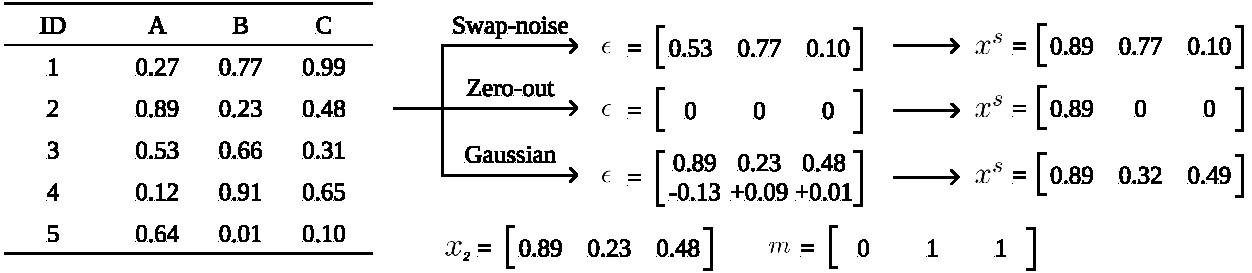
\includegraphics[width=1\linewidth]{masking-example}
    \caption{Examples of synthetic observations generated with different
        masking approaches.
    }~\label{fig:masking-example}
\end{figure}

Masking modifies the original perturbation based approach by introducing a
binomial mask vector, $m = [m_1, \ldots, m_d]^\bot \in \{0,1\}^d, m_i \sim
\text{Bern}(p_m)$ and the generation mechanism is defined as $x^s = (1 -
m)\odot x_i + m \odot \epsilon$~\cite{yoon2020vime}. The $\epsilon$ variable
is defined according to the perturbation used. The Gaussian approach generates
the noise vector as $\epsilon = x_i + \epsilon'$, where $e_i' \sim
\mathcal{N}(\cdot, \cdot), \forall e_i' \in \epsilon'$. The swap-noise
approach shuffles the feature values from all observations to form
$\epsilon$, while the zero-out noise approach sets all $\epsilon$ values to
zero. Intuitively, the masking technique modifies an observation's feature
values with probability $p_m$, instead of adding perturbations over the
entire observation. Figure~\ref{fig:masking-example} shows a visual depiction
of the masking technique.

\subsection{Probability Density Function Mechanisms}

The Gaussian generative model, despite unfrequently used when compared to the
remaining Probaility Density Function mechanisms discussed in this subsection,
is an essential building block for these mechanisms. In particular, we focus
on the multivariate gaussian approach, which follows near-Gaussian
distribution assumptions, which is rarely reasonable on the input space.
However, for high-dimensional data, it is possible to motivate this approach
via the \textit{Diaconis-Freedman-Meckes} effect~\cite{meckes2012projections},
which states that high-dimensional data projections generally follow a nearly
Gaussian distribution. The Gaussian generative model produces synthetic data
from a Gaussian distribution $x^s \sim \mathcal{N}(\mu, \Sigma)$, where $\mu
\in \mathbb{R}^d$ is a vector with the features' means and $\Sigma \in
\mathbb{R}^{d \times d}$ is the covariance matrix. It follows the following
density function~\cite{chanyaswad2019ron}:

\begin{equation}\label{eq:gaussian}
    f(x) =
    \frac{1}{\sqrt{(2\pi)^d\text{det}(\Sigma)}}\text{exp}\left(-\frac{1}{2}(x-\mu)^T\Sigma^{-1}(x-\mu)\right)
\end{equation}

Consequently, to define a Gaussian generative model it is only necessary to
estimate the dataset's mean and covariance matrix.

A Gaussian mixture model (GMM) comprises several Gaussian distributions that
aim to represent subpopulations within a dataset. Its training procedure
allows the model to iteratively learn the subpopulations using the Expectation
Maximization algorithm. A GMM becomes more appropriate than the Gaussian
generative model when the data is expected to have more than one
higher-density regions, leading to a poor fit of unimodal Gaussian models.

Kernel Density Estimation (KDE) methods use a kernel function to estimate the
density of the dataset's distribution at each region of the input/latent
space. Despite the various kernel options, the Gaussian kernel is commonly
used for synthetic data generation~\cite{tang2015kerneladasyn}. The general
kernel estimator is defined as follows: 

\begin{equation}
    \hat{p}(x) = \frac{1}{N+h}
    \sum_{i=1}^{N}K\left(\frac{x-x_i}{h}\right)
\end{equation}

Where $N = |\mathcal{D}|$, $h$ is a smoothing parameter known as bandwidth and
$K$ is the kernel function. The Gaussian kernel is defined as follows:

\begin{equation}
    G_i(x) = K\left(\frac{x-x_i}{h} \right) = \frac{1}{(\sqrt{2\pi} h)^d} 
    \text{exp}\left(-\frac{1}{2}\frac{(x-x_i)^T(x-x_i)}{h}\right) 
\end{equation}

Therefore, the Gaussian KDE approach can also be expressed as $\hat{p}(x) =
\frac{1}{N+h}\sum_{i=1}^{N}G_i(x)$, while the data is sampled from the
estimated probability distribution. Figure~\ref{fig:pdf-example} shows a
visualization of the PDF mechanisms discussed, applied to a mock dataset.

\begin{figure}
	\centering
	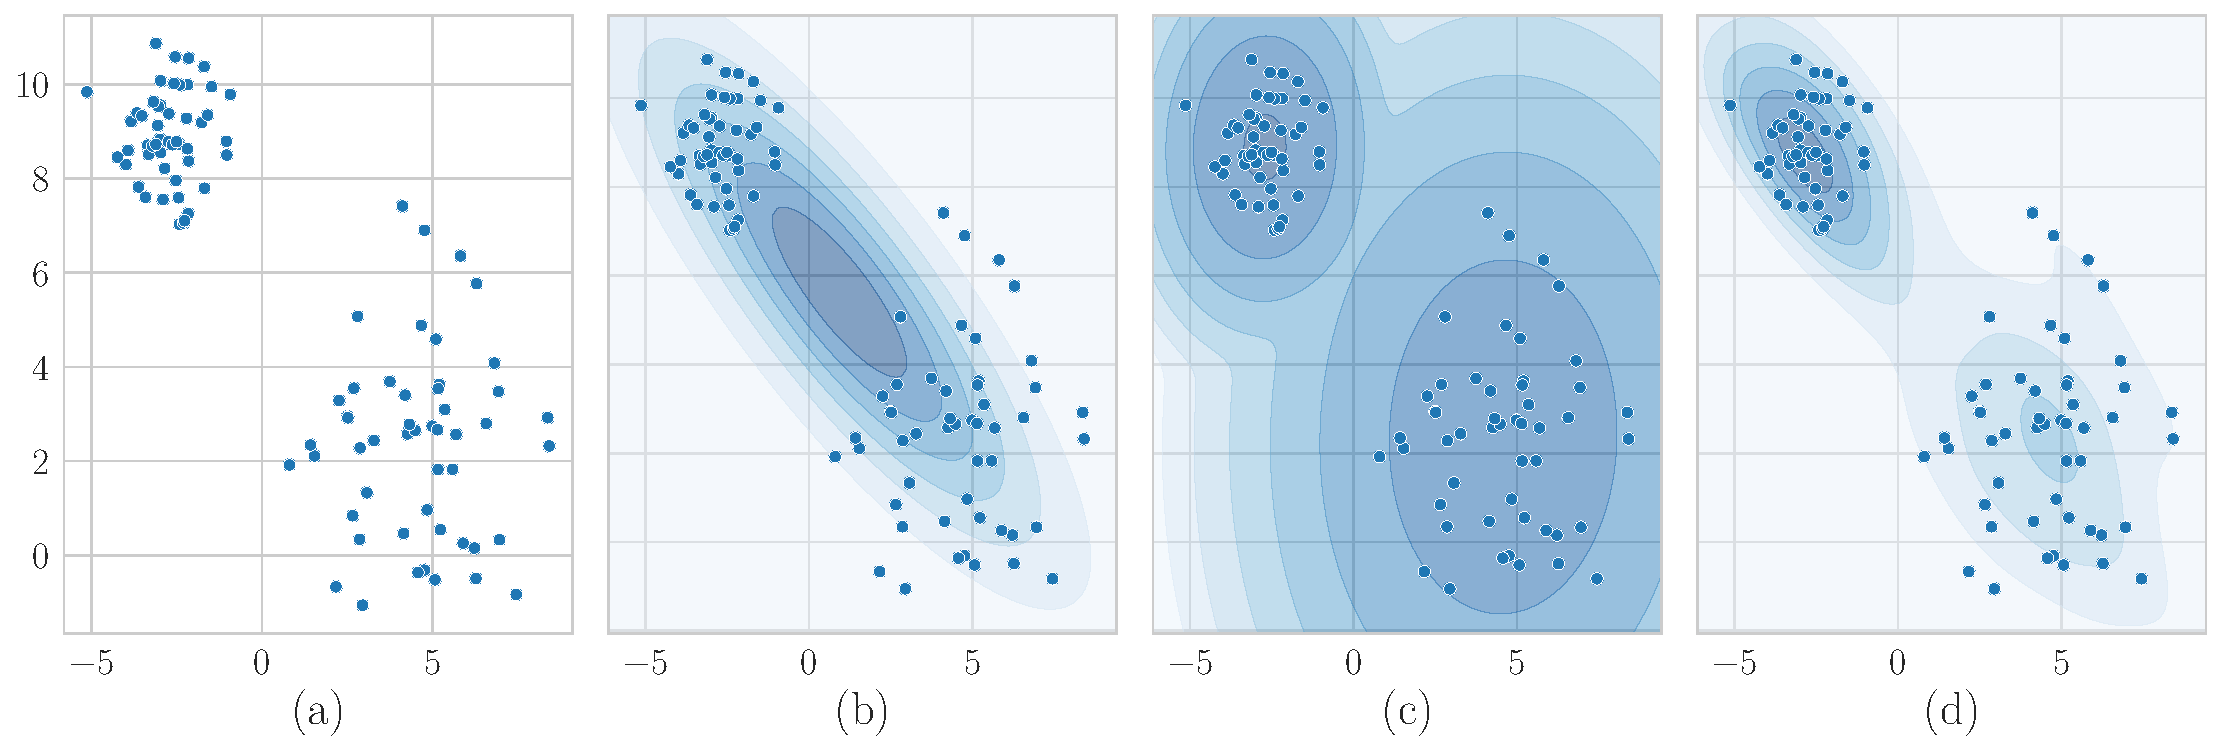
\includegraphics[width=1\linewidth]{pdf-example}
    \caption[Examples of PDF mechanisms fitted to a mock dataset.]{%
        Examples of PDF mechanisms fitted to a mock dataset. Legend: (a)
        Original dataset, (b) Gaussian generative model, (c) Gaussian Mixture
        Model and (d) Gaussian Kernel Density Estimation.
    }~\label{fig:pdf-example}
\end{figure}

\subsection{Probabilistic Graphical Models}

A Bayesian network can be thought of as a collection of as a collection of
conditional distributions. It represents the joint probability distribution
over the cross-product of the feature domains in $\mathcal{D}$. It is a
directed acyclic graph that represents $\mathcal{D}$'s features as nodes and
their conditional dependencies as directed edges. The set of features pointing
directly to feature $v \in V, d=|V|$ via a single edge are known as the parent
variables, $pa(v)$. A Bayesian network calculates $p(x)$ as the product of the
individual density functions, based on the conditional probabilities of the
parent variables:

\begin{equation}
    p(x) = \prod_{v \in V} p(x_v | x_{pa(v)})
\end{equation}

Since the construction of a directed acyclic graph can be labor intensive,
different ML approaches were developed for the learning of these
structures~\cite{yu2019dag}. Bayesian networks can be used for synthetic data
generation when the relationship between variables is known (or can be
learned) and when the data is high dimensional, making the sampling process
non-trivial.

Random walk algorithms comprise the general process of iterating through a set
of random steps. Although uncommon, random walk approaches may be used to
sample data. The random walk approach described in \citet{zhang2014rwo} uses
the Gaussian noise mechanism over minority class observations to create
synthetic observations. The Gibbs sampling mechanism also performs a random
walk by iterating through sampled feature values.

Gibbs sampling is a Markov Chain Monte Carlo algorithm that iteratively
samples a synthetic observation's feature values. It is a suitable method to
sample synthetic data from a Bayesian network. The process starts with an
initial observation selected from $\mathcal{D}$, $x_0$ and is used to begin
the sampling process. In its original format, the sampling of each feature
value $v$ in $x^s_i$ is conditioned by $x^s_{i-1}$ and the feature values
already sampled from $x^s_i$, such that $x^s_{i, v} \sim p(x^s_{i, v} |
x^s_{i, 1}, \ldots, x^s_{i, v-1}, x^s_{i-1, v+1}, \dots, x^s_{i-1, d})$.
Therefore, Gibbs sampling is a special case of the Metropolis-Hastings
algorithm.

\subsection{Linear Transformations}

Linear interpolation mechanisms can be split into two subgroups: between and
within-class interpolation. Both mechanisms follow a similar approach; they
use a scaling factor $\lambda$, typically sampled from either
$\mathcal{U}(0,1)$ or $\text{Beta}(\alpha, \alpha)$: 

\begin{equation}~\label{eq:interpolation}
    x^s = \lambda x_i + (1-\lambda)x_j = x_j + \lambda(x_i - x_j)
\end{equation}

The within-class interpolation mechanism selects two observations from the
same class, while the between-class interpolation mechanism selects two
observations from different classes and also interpolates the one-hot encoded
target classes $y_i$ and $y_j$. However, the approach to select observations
might vary according to the ML task and data generation algorithm. For
example, most SMOTE-based methods select a center observation and a random
observation within its $k$-nearest neighbors belonging to the same class,
while the Mixup method selects two random observations, regardless of their
class membership.

\begin{figure}
	\centering
	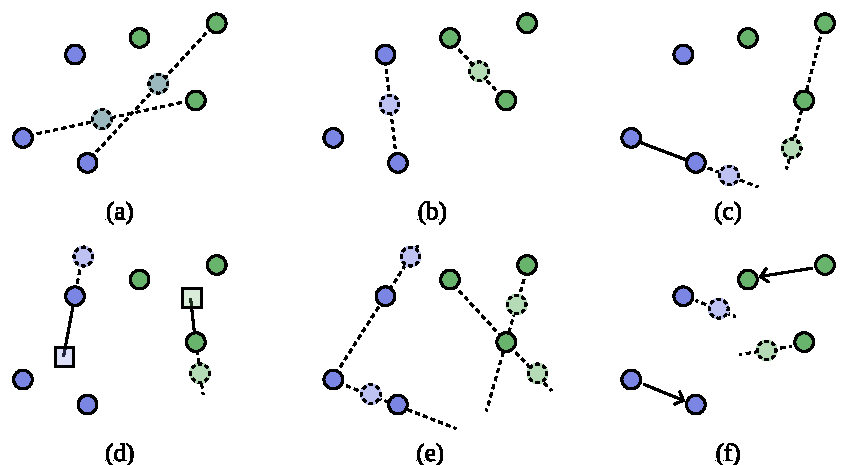
\includegraphics[width=.7\linewidth]{linear-transformations}
    \caption[Examples of linear transformation mechanisms.]{%
        Examples of linear transformation mechanisms. Legend: (a)
        Between-class interpolation, (b) Within-class interpolation, (c)
        Observation-based extrapolation, (d) Hard extrapolation, (e)
        Combination of interpolation and extrapolation and (f) Difference
        transform.
    }~\label{fig:linear-transformations}
\end{figure}

The observation-based linear extrapolation mechanism modifies
Equation~\ref{eq:interpolation} such that $x^s = x_i + \lambda(x_i - x_j)$,
while the hard extrapolation mechanism uses the mean of a class' observations,
$\mu^c$ and a randomly selected observation to generate $x^s = x_i^c +
\lambda(x_i^c - \mu^c)$. Some methods also combine both interpolation and
extrapolation. This can be achieved using Equation~\ref{eq:interpolation} and
modifying $\lambda$'s range to either decreasing its minimum value below zero
or increasing its maximum value above one.

The difference transform mechanism uses two observations to compute a
translation vector (multiplied by the scaling factor $\lambda$) and apply it on
a third observation:
\begin{equation}
    x^s = x_i + \lambda(x_j - x_k)
\end{equation}

Although there are various linear transformation mechanisms in the literature,
the majority of the studies applied linear interpolation mechanisms.
Within-class interpolation was frequently found in oversampling methods, while
between-class interpolation was found most often in regularization methods. A
depiction of the linear transformation mechanisms found in the literature are
presented in Figure~\ref{fig:linear-transformations}.

\subsection{Geometric Transformations}

Overall, geometric transformation mechanisms were not frequently found in the
literature. They are primarily used to develop Mixup or SMOTE-based variants.
Figure~\ref{fig:geometric-transformations} shows a visual example of the
related mechanisms.

The hypersphere mechanism generates data within a distorted, n-dimensional
hyperspheroid. It is formed using an observation to define the center of
the geometry and another to define its edge.
It is defined with two hyperparameters, the deformation
factor, $\alpha_{def} \in [0, 1]$, and the truncation factor, $\alpha_{trunc}
\in [-1, 1]$. The deformation factor deforms the hypersphere into an elliptic
shape, where $\alpha_{def}=1$ applies no deformation and $\alpha_{def}=0$
creates a line segment. The truncation factor limits the generation area of
the hyperspheroid within a subset of the hypersphere, where $\alpha_{trunc}=0$
applies no truncation, $\alpha_{trunc}=1$ uses the half of the area between
the two selected observations and $\alpha_{trunc}=-1$ uses the opposing area.
In Figure~\ref{fig:geometric-transformations}a, the two generation areas were
formed using approximately $\alpha_{trunc} = \alpha_{def} = 0.5$.

The triangular mechanism selects three observations to generate $x^s =
\lambda_ix_i + \lambda_jx_j + (1-\lambda_i-\lambda_j)x_k$, where $\lambda_i,
\lambda_j \sim \mathcal{U}(0, \alpha)$, $\alpha \in (0, 0.5]$. The
hyperrectangle mechanism uses an approach similar similar to
Equation~\ref{eq:interpolation}. However, the scaling factor is changed into a
scaling vector, $\Lambda = [\lambda_1,\dots,\lambda_d ] \in [0,1]^d, \lambda_i
\sim \text{Beta}(\alpha, \alpha)$, where $\alpha$ is a hyperparameter used to
define the Beta distribution. A synthetic observation is generated with $x^s =
\Lambda \odot x_i + (1-\Lambda) \odot x_j$, where $\odot$ denotes the Hadamard
product. This operation originates a generation area like the ones presented
in Figure~\ref{fig:geometric-transformations}c.

\begin{figure}
	\centering
	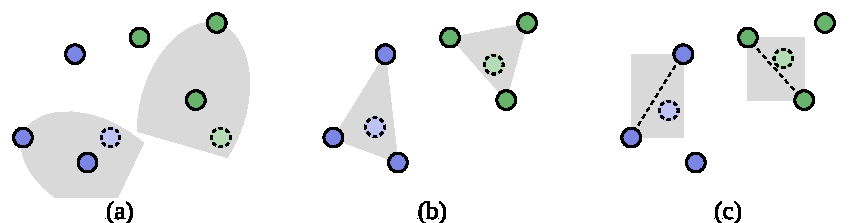
\includegraphics[width=.7\linewidth]{geometric-transformations}
    \caption[Examples of geometric transformation mechanisms.]{%
        Examples of geometric transformation mechanisms. Legend: (a)
        hypersphere mechanism, (b) triangular mechanism and (c)
        hyperrectangle mechanism.
    }~\label{fig:geometric-transformations}
\end{figure}

\subsection{Neural Networks}

Generative Adversarial Network (GAN) architectures are structured as a minimax
two-player game composed of two models, a generator and a discriminator. Both
models are trained simultaneously throughout the learning phase, to learn to
generate data with similar statistical properties when compared to the
original data. The generative model captures the data distribution, while the
discriminator estimates the probability of an observation coming from the
training data. The goal of the generator model is to produce synthetic
observations that are capable of fooling the discriminator, making it
difficult for the discriminator to distinguish real from synthetic
observations. Although they were originally developed in an unsupervised
learning setting~\cite{goodfellow2020generative}, subsequent contributions
proposed GANs with several different architectures, for semi-SL, supervised
learning (for both regularization and oversampling) and reinforcement
learning.

An autoencoder (AE) is a type of neural network architecture that learns
manifold representations of an input space. These models are typically trained
by regenerating the input and are designed with a bottleneck in the hidden
layers that corresponds to the learned latent space. It contains two parts,
an encoder and a decoder. The encoder transforms the input data into
lower-dimensional representations (\textit{i.e.}, the latent space), while
the decoder projects these representations into the original input space.
Since it was first proposed~\cite{ackley1985learning}, many variants were
developed for multiple applications. However, based on the literature found,
the variational AE architecture appears to be the most popular approach.

\section{Evaluating the Quality of Synthetic Data
}\label{sec:evaluating-synthetic-data-synth}

The vast majority of synthetic data generation models are evaluated on a ML
utility basis. Compared to research on the development of actual synthetic
data generation algorithms, there is a general lack of research on the
development of metrics to evaluate their quality beyond performance metrics
such as Overall Accuracy (OA) or F1-score. One motivation to do this is the
ability to anticipate the quality of the data for the target task before
training a ML classifier, which may be expensive and time-consuming.  This is
a challenging problem, since the usefulness of synthetic data generators
depend on the assumptions imposed according to the dataset, domain and ML
problem~\cite{chundawat2022tabsyndex}. This section focuses on the main
evaluation approaches found in the literature beyond classification
performance, as well as recently proposed methods. For a more comprehensive
analysis of performance metrics for synthetic data evaluation, the reader is
referred to~\cite{dankar2022multi} and~\cite{theis2016note}.

The GANBLR model~\cite{zhang2021ganblr} was evaluated on three aspects: (1) ML
utility, (2) Statistical similarity, and (3) Interpretability. In
\citet{xu2019modeling}, the authors evaluate the CTGAN and TVAE models using a
likelihood fitness metric (to measure statistical similarity) and ML efficacy
(\textit{i.e.}, utility). \citet{hittmeir2019utility} evaluate synthetic data
generators using a 2-step approach: Similarity comparison and data utility.
According to \citet{alaa2022faithful}, the evaluation of generative models
should quantify three key aspects of synthetic data:

\begin{enumerate}

    \item Fidelity. The synthetic observations must resemble real
        observations; 

    \item Diversity. The synthetic observations should cover $\mathcal{D}$'s
        variability;

    \item Generalization. The synthetic observations should not be copies of
        real observations;

\end{enumerate}

Ensuring these properties are met will secure the objectives defined in
Section~\ref{sec:problem-formulation-synth}: $\mathbb{P}^s \approx
\mathbb{P}$ and $x_i \neq x_j \forall x_i \in \mathcal{D} \wedge x_j \in
\mathcal{D}^s$.

The effective evaluation of synthetic data generation methods is a complex
task. A good performance with respect to one evaluation method does not
necessarily imply a good performance on the primary ML task, results from
different evaluation methods seem to be independent, and evaluating the models
directly onto the target application is generally
recommended~\cite{theis2016note}. Therefore, each evaluation procedure must be
carefully implemented and adapted according to the use case.

\subsection{Quantitative approaches}

The Kullback-Leibler (KL) divergence (and equivalently the log-likelihood) is a
common approach to evaluate generative models~\cite{theis2016note}. Other
commonly used metrics, like Parzen window estimates, appear to be a generally
poor quality estimation method and are not recommended for most
applications~\cite{theis2016note}. KL divergence is defined as follows:

\begin{equation}
    D_{KL}(P||Q) = \sum_{x\in\mathcal{X}}P(x)\log{\frac{P(x)}{Q(x)}}
\end{equation}

Where $\mathcal{X}$ is a probability space, $P$ and $Q$ are estimated
probability distributions based on $\mathbb{P}$ and $\mathbb{P}^s$,
respectively. The KL divergence is a non symmetric measurement that represents
how a reference probability distribution ($P$) differs from another
($Q$). A $D_{KL}$ close to zero means $Q$ is similar to $P$. However, metrics
like the KL divergence or the log-likelihood are generally difficult to
interpret, do not scale well for high dimensional data and fail to
highlight model failures~\cite{alaa2022faithful}. Another related metric, used
in~\cite{zhao2021ctab}, is the Jensen-Shannon (JS) divergence. It consists of
a symmetrized and smoothed variation of the KL divergence. Having
$M=\frac{P+Q}{2}$, it is calculated as:

\begin{equation}
    D_{JS}(P||Q) = \frac{D_{KL}(P||M) + D_{KL}(Q||M)}{2}
\end{equation}

The Wasserstein Distance is another relevant metric to estimate the
distance between two distribution functions. It was also used to develop GAN
variants since it improves the stability in the training of
GANs~\cite{gulrajani2017improved, goncalves2020generation}.

In past literature, the propensity score was considered an appropriate
performance metric to measure the utility of masked data~\cite{woo2009global}.
This metric is estimated using a classifier (typically a logistic regression)
trained on a dataset with both the original and synthetic data, using as
target the source of each observation (synthetic or original). The goal of
this classifier is to predict the likelihood of an observation to be
synthetic. Therefore, this approach guarantees observation-level insights
regarding the faithfulness of each observation. \citet{woo2009global} suggest
a summarization of this metric, also defined as the propensity Mean Squared Error
(pMSE)~\cite{chundawat2022tabsyndex}:

\begin{equation}~\label{ep:propensity}
    U_p = pMSE = \frac{1}{N} \sum^N_{i=1}{(\hat{p}_i - c)}^2
\end{equation}

Where $N = |\mathcal{D} \cup \mathcal{D}^s|$, $c = \frac{|\mathcal{D}^s|}{N}$
and $\hat{p}_i$ is the estimated propensity score for observation $i$. When a
synthetic dataset is indistinguishable from real data, $pMSE$ will be close to
zero. Specifically, when the data source is indistinguishable, the expected
pMSE is given by~\cite{snoke2018general}:

\begin{equation}
    E(pMSE) = \frac{(k-1)(1-c)^2c}{N}
\end{equation}

Where $k$ is the number of parameters in the logistic regression model
(including bias). When the synthetic dataset is easily distinguishable from
the original dataset, $U_p$ will be close to ${(1-c)}^2$.
\citet{dankar2021fake}, established a generally consistent, weak negative
correlation between $U_p$ and OA\@.

\citet{chundawat2022tabsyndex} proposed TabSynDex to address the lack of
uniformity of synthetic data evaluation, which can also be used as a loss
function to train network-based models. It is a single metric evaluation
approach bounded within $[0,1]$ that consists of a combination between (1) the
relative errors of basic statistics (mean, median and standard deviation), (2)
the relative errors of correlation matrices, (3) a pMSE-based index, (4) a
support coverage-based metric for histogram comparison and (5) the performance
difference in a ML efficacy-based metric between models trained on real and
synthetic data.

The three-dimensional metric proposed by~\citet{alaa2022faithful} presents an
alternative evaluation approach. It combines three metrics
($\alpha$-Precision, $\beta$-Recall and Authenticity) for various application
domains. It extends the Precision and Recall metrics defined
in~\cite{sajjadi2018assessing} into $\alpha$-Precision and $\beta$-Recall,
which are used to quantify fidelity and diversity. Finally, the authenticity
metric is estimated using a classifier that is trained based on the distance
(denoted as $d$) between $x^s$ and its nearest neighbor in $\mathcal{D}$,
$x_{i^*}$; if $d(x^s, x_{i^*})$ is smaller than the distance between $x_{i^*}$
and its nearest neighbor in $\mathcal{D}\backslash \{x_{i^*}\}$, $x^s$ will
likely be considered unauthentic. This approach provides a three fold
perspective over the quality of $\mathcal{D}^s$ and allows a sample-level
analysis of the generator's performance. Furthermore, there is a relative
trade-off between the two metrics used to audit the generator and the
synthetic data; a higher $\alpha$-Precision score will generally correspond to
a lower Authenticity score and vice versa.

A less common evaluation approach is to attempt to replicate the results of
studies using synthetic data~\cite{el2020seven, benaim2020analyzing,
rosenblatt2022epistemic}. Another method is the computation of the
average distance among synthetic observations and their nearest neighbors
within the original dataset~\cite{hittmeir2019utility}. The Confidence
Interval Overlap and Average Percentage Overlap metrics may be used to
evaluate synthetic data specifically for regression
problems~\cite{khan2022utility, karr2006framework}.

\subsection{Qualitative approaches}

One of the qualitative approaches found in the literature is the comparison of
the features' distributions with synthetic data and the original data using
histogram plots~\cite{hittmeir2019utility}. This comparison can be
complemented with the quantification of these distribution
differences~\cite{el2020seven}. A complementary approach is the comparison of
correlation matrices via heat map plots~\cite{hittmeir2019utility}.

Another way to assess the quality of synthetic data is the subjective
assessment by domain experts~\cite{el2020seven}. The goal of such test is to
understand whether domain experts are able to distinguish synthetic from real
data, which could be quantified with classification performance metrics. A low
classification performance implies synthetic data that is difficult to
distinguish from real data.

\section{Discussion}\label{sec:discussion-synth}

The generation of tabular and latent space synthetic data has applications in
multiple ML tasks and domains. Specifically, we found six areas that were
shown to benefit from synthetic data: data privacy, regularization,
oversampling, active learning, semi-supervised learning and self-supervised
learning. Synthetic data may be used either as an accessory task to improve a
ML model's performance over a primary task (\textit{e.g.}, regularization and
oversampling), an intermediate task (\textit{e.g.}, feature extraction), or as
a final product itself (\textit{e.g.}, data anonymization). The analysis of
data generation algorithms for each relevant learning problem led to the
proposal of a general purpose taxonomy primarily focused on the underlying
mechanisms used for data generation. We characterized every algorithm
discussed in this work into four categories: (1) architecture, (2) application
level, (3) data space and (4) scope. The successful implementation of
synthetic data generation generally requires a few considerations:

\begin{enumerate}

    \item Ensuring the dataset's features are comprised within similar, fixed
        boundaries. For example, any method using a neighbors-based approach
        will rely on distance measurements (typically the euclidean distance),
        which is sensitive to the scale of the data and a nearest-neighbors
        estimation may vary depending on whether the data was scaled \textit{a
        priori}. This can be achieved with data scaling. 

    \item Various generation mechanisms require a manifold. There are two
        approaches to address non-manifold input data: (1) Adopt methods
        sensitive to the presence of non-metric features, or (2) project the
        input data into a manifold (\textit{i.e.}, a latent space).

    \item The smoothness assumption is prevalent in linear and
        perturbation-based data generation mechanisms. If a classification
        problem has low class separation and difficult to solve, the choice in
        the design of the generator algorithm is also difficult. Generally,
        generation algorithm with a global scope might adapt better to
        classification problems with low separability. On the other hand,
        problems with higher separability might require a definition of more
        uniform decision boundaries to prevent overfitting, which can be
        achieved with generation algorithms with a local scope.

    \item Considering the trade-off between performance and computational
        power. It is generally understood that computationally-intensive
        approaches tend to produce synthetic data with higher quality. When
        trained properly, neural network mechanisms typically lead to
        synthetic data that is more difficult to distinguish compared to the
        remaining approaches. Geometric mechanisms have also achieved good
        results but often require a careful tuning of their hyperparameters.
        Linear and perturbation mechanisms do not require much training and
        use less hyperparameters, but have been know for often producing low
        diversity synthetic data (\textit{vis a vis} the original dataset).

\end{enumerate}

This work focused primarily on the mechanisms used to generate synthetic
observations; preprocessing, learning phase design, latent space learning and
ML task-specific contributions were secondary objectives for analysis.
Consequently, understanding of how the constraints within each task condition
the choice and design of the synthetic data generator is a subject of future
work.

Throughout the analysis of the literature, we identified six types of
generation mechanisms and discuss more specific methods used in classical and
state-of-the-art techniques. Techniques for data privacy via synthetic data
rely primarily on perturbation mechanisms, PDFs, PGMs and Neural networks.
Regularization approaches frequently employ Linear mechanisms. Other less
commonly used mechanisms are PGMs, Neural network approaches, geometric and
perturbation mechanisms. Various Oversampling algorithms have been proposed
using each of the mechanisms found. However, the most prevalent mechanisms
used were linear-based. AL methods rarely employ synthetic data. The few
studies found employ primarily linear and geometric mechanisms, and a minority
used AE models for latent space augmentation. Most Semi-SL methods used
perturbation and linear mechanisms, while geometric mechanisms are rarely
used. All tabular Self-SL methods used perturbation mechanisms. 

% Recommendations for data evaluation
Designing an approach to measure the quality of synthetic data depends on the
target ML problem. A wholistic evaluation approach for synthetic data should
consider the analysis of (1) ML utility, (2) Statistical similarity, (3)
interpretability. The analysis of statistical similarity can be further
divided into (1) fidelity, (2) diversity and (3) generalization.  However,
balancing the analysis between these three perspectives is not a
straightforward task. For example, duplicating a dataset to form a synthetic
dataset will result into the best possible fidelity and diversity, but bad
generalization. Overall, there is a paucity of research into the development
of comprehensive analyses of synthetic data, as well as understanding the
balance between the different types of analyses.

\section{Future Work}\label{sec:future-work-synth}
% TODO: maybe rename to "Research gaps and future directions"?

As discussed throughout our analysis, it appears the synthetic data generation
research is generally isolated within ML problems and/or domains, even though
all of these areas integrate synthetic data in its core. Given the breadth and
complexity of input-level and latent-level data generation mechanisms, it is
increasingly important to find an \textit{a priori} approach to efficiently
determine appropriate data generation policies and techniques. However, the
complexity of this task is determined by various factors: different data
types, ML problems, model architectures, computational resources, performance
metrics and contextual constraints. Auto-augmentation and meta learning aim to
address this challenge and are still subject to active research.

It is understood that, if learned properly, the latent space is expected to be
convex and isotropic. In that case, using linear generation techniques in the
latent space would produce synthetic data without introducing
noise~\cite{cheung2020modals}. However, it is unclear which types of
model/architectures and training procedures contribute to the learning of a
good latent space according to the context. Furthermore, we found a limited
amount of research on tabular data augmentation using auto-encoder
architectures. Although there are studies performing data augmentation on
tabular data in various domains~\cite{delgado2021deep}, defining the
architecture and learning phase of an AE is not an intuitive task. Generally,
autoencoders are used to learn a manifold for more complex data types. As long
as the method used to generate the latent space is appropriate, the methods
discussed in this study could be used in the latent space regardless of the
type of data.

The quality of synthetic data generation in high-dimensional scenarios appears
as a prevailing limitation in various applications, especially within linear
and geometric mechanisms. This limitation can be addressed with dimensionality
reduction techniques, as well as latent space learning.  However, research on
data generation in the latent space is mostly focused on GAN architectures,
which require significant computational power. Other methods to learn manifold
latent spaces could be explored to address this limitation.

It remains an open question which generation mechanisms, or types of
mechanisms, create better synthetic data~\cite{cheung2020modals}. Although
there is not necessarily a one-size-fits-all solution, a general set of rules
of thumb could be explored, such as understanding how certain characteristics
of a problem will affect the choice of the generation policy, which types of
mechanisms are more appropriate for different types of dataset, ML model
architecture, domains and target ML problem, or the trade-offs between the
different types of generation mechanism. A better understanding of the
relationship between recently proposed methods for evaluating synthetic data
(as discussed in Section~\ref{sec:evaluating-synthetic-data-synth}) and the
performance on the target ML problem might contribute to answer this question.
Furthermore, determining the use cases, quality and general performance of
data generation on the input, latent and output space should be further
developed. Finally, it still unclear \text{why} synthetic data generation
works for each of the ML tasks discussed. Research on this topic lacks depth
and fails to address the theoretical underpinnings~\cite{feng2021survey,
dao2019kernel}.

% data privacy
The evaluation of anonymization techniques lack standardized, objective and
reliable performance metrics and benchmark datasets to allow an easier
comparison across classifiers to evaluate key aspects of data anonymization
(resemblance, utility, privacy and performance). These datasets should contain
mixed data types (\textit{i.e.}, a combination of categorical, ordinal,
continuous and discrete features) and the metrics should evaluate the
performance of different data mining tasks along with the anonymization
reliability. This problem appears to be universal across domains. For example,
\citet{hernandez2022synthetic} observed the lack of a universal method or
metric to report the performance synthetic data generation algorithms for
tabular health records. Therefore, in order to facilitate the usage of these
techniques in industry domains, these benchmarks must also be
realistic. \citet{rosenblatt2020differentially} attempts to address this
problem by proposing a standardized evaluation methodology using standard
datasets and real-world industry applications.

% Regularization in supervised learning
Unlike data privacy solutions, studies on data augmentation techniques
generally do not consider the similarity/dissimilarity of synthetic data. The
study of quality metrics for supervised learning may reduce computational
overhead and experimentation time. Only one study related to the relationship
of quality metrics and performance in the primary ML task was found
in~\cite{dankar2021fake}, which was done only for the pMSE metric.

Neural network mechanisms typically involve a higher computational cost
compared to the remaining types of mechanisms. This problem is further
aggravated with their inconsistent performance, since different
initializations may result in very different performances. This problem may be
observed in~\cite{douzas2018effective}. More generally, latent space
representations of training data raises the challenge of interpretability; the
ability to interpret latent space representations could guide the design of
data generation techniques. 

In non-tabular data domains, a common approach for data augmentation is the
combination of several data augmentation methods to increase the
diversification of synthetic data. This is true for both text
classification~\cite{bayer2021survey} and image
classification~\cite{grill2020bootstrap}. However, for tabular data, no
studies were found that discuss the potential of ensembles of generation
mechanisms on tabular data, \textit{i.e.}, understanding how selecting with
different probabilities different generation mechanisms to generate synthetic
data would affect the performance of the primary ML task. The formalization
and analysis carried out in this work, regarding the different types of
synthetic data generation mechanisms and quality metrics for latent and
tabular synthetic data at an observation level, may facilitate this work.


% oversampling
Various oversampling methods have been proposed to address imbalanced learning
limitations. However, there is still a major limitation in the literature
regarding the oversampling of datasets with mixed data types or with
exclusively non metric features at the input space. In addition, 
the research on oversampling using PDFs or PGMs is scarce.

To the best of our knowledge, research on few-shot learning for tabular data
is scarce. Few-shot learning research using synthetic data generation
techniques has been extensively developed using
image~\cite{cubuk2019autoaugment, zhao2019data} and text
data~\cite{zhou2021flipda}, but they are rarely adapted or tested for tabular
data. One of the few studies found achieved a good performance in both
few-shot and zero-shot learning through the adaptation of a Large Language
model for tabular data~\cite{hegselmann2022tabllm}. 

% % Self-supervised Learning
% There is no clear understanding of the most appropriate data augmentation
% techniques used to train self-supervised models and how their behavior and
% performance varies according to the data generation method used.

% Societal challenges raised by data generation (?)
% Systematic bias

Oversampling does not seem to be a relevant source of bias in behavioral
research and does not appear to have an appreciably different effect on
results for directly versus indirectly oversampled
variables~\cite{hauner2014latent}. However, most oversampling methods do not
account for the training dataset's distribution, which is especially important
for features with sensitive information (\textit{e.g.}, gender or ethnicity).
Therefore, the application of oversampling methods on user data may further
increase the bias in classification between gender or ethnicity groups.

Finally, various synthetic data generation algorithms are research-based, and
might not be usable or feasible to be implemented by
practitioners~\cite{bayer2021survey}. One way to address this problem is to
publish the code developed, and ideally make them available as open source
libraries for out-of-the-box usage.

% \subsection{Research directions}

% similarities between mixup and SMOTE, and an intermediate solution that can
% be further explored to use the mixup approach on tabular data
% (Geometric-SMOTE selection mechanism)

% Quantifying the quality of the generated data:
% 
% \begin{enumerate}
%     \item Realistic
%     \item Similarity
%     \item Usefulness (determine purpose and relevant performance metric)
%     \item Understand the relationship between the 3 factors
% \end{enumerate}

\section{Conclusions}\label{sec:conclusions-synth}

This literature review analyses various synthetic data generation-based
algorithms for tabular data, with a focus on external level applications.
Since synthetic data generation is a crucial step for various ML applications
and domains, it is essential to understand and compare which techniques and
types of algorithms are used for each of these problems. The usage of
synthetic data is an effective approach to better prepare datasets and ML
pipelines for a wide range of applications and/or address privacy concerns.
Our work proposed a taxonomy based on four key characteristics of generation
algorithms, which was used to characterize 70 data generation algorithms
across six ML problems. This analysis resulted in the categorization and
description of the generation mechanisms underlying each of the selected
algorithms into six main categories. Finally, we discussed several techniques
to evaluate synthetic data, as well as general recommendations and research
gaps based on the insights collected throughout the analysis of the
literature.

Despite the extensive research developed on various different methods for
synthetic data generation, there are still open questions regarding the
theoretical underpinnings of synthetic data adoption for each of the
techniques, as well as limitations in the different types of generation
mechanisms and evaluation procedures. However, the empirical work presented in
the literature show significant performance improvements and promising
research directions for future work.

\thesischapter{%
    Geometric SMOTE for Imbalanced Datasets with Nominal and Continuous Features
}{%
    Submitted as Joao Fonseca, Fernando Bacao, to a Q1 Journal, 2023
}~\label{chp:gsmotenc}
\graphicspath{{figures/gsmotenc/}}

\begin{adjustwidth}{30pt}{30pt}

    Imbalanced learning can be addressed in 3 different ways: resampling,
    algorithmic modifications and cost-sensitive solutions. Resampling, and
    specifically oversampling, are more general approaches when opposed to
    algorithmic and cost-sensitive methods. Since the proposal of the
    Synthetic Minority Oversampling TEchnique (SMOTE), various SMOTE variants
    and neural network-based oversampling methods have been developed.
    However, the options to oversample datasets with nominal and continuous
    features are limited. We propose Geometric SMOTE for Nominal and
    Continuous features (G-SMOTENC), based on a combination of G-SMOTE and
    SMOTENC. Our method modifies SMOTENC's encoding and generation mechanism
    for nominal features while using G-SMOTE's data selection mechanism to
    determine the center observation and k-nearest neighbors and generation
    mechanism for continuous features. G-SMOTENC's performance is compared
    against SMOTENC's along with two other baseline methods, a
    State-of-the-art oversampling method and no oversampling. The experiment
    was performed over 20 datasets with varying imbalance ratios, number of
    metric and non-metric features and target classes. We found a significant
    improvement in classification performance when using G-SMOTENC as
    the oversampling method. An open-source implementation of G-SMOTENC is
    made available in the Python programming language.

\end{adjustwidth}

\vspace{.5cm}
\textbf{Keywords:} Imbalanced Learning; Oversampling; SMOTE; Data Generation;
Nominal Data

\section{Introduction}~\label{sec:introduction-gsmotenc}

% the problem of imbalanced learning
Various Machine Learning (ML) tasks deal with highly imbalanced datasets, such
as fraud transactions detection, fault detection and medical
diagnosis~\cite{tyagi2020sampling}. In these situations, predicting false
positives is often a more acceptable error, since the class of interest is
usually the minority class~\cite{vuttipittayamongkol2021class}. However, using
standard ML classifiers on imbalanced datasets induces a bias in favor of the
classes with the highest frequency, while limiting the predictive power on
lower frequency classes~\cite{lopez2013insight, das2018handling}. This effect
is known in the ML community as the Imbalanced Learning problem.

% existing approaches to address imbalanced learning
Imbalanced learning involves a dataset with two or more target classes with
varying class frequencies. The minority class is defined as the class with the
least amount of observations and the majority class is the one with the
highest amount of observations~\cite{kaur2019systematic}. There are three main
approaches to address imbalanced learning~\cite{Fernandez2013}: 

\begin{enumerate}
    \item Cost-sensitive solutions attribute a higher misclassification cost
        to the minority class observations to minimize higher cost errors;
    \item Algorithmic level solutions modify ML classifiers to improve the
        learning of the minority class;
    \item Resampling solutions generate synthetic minority class observations
        and/or remove majority class observations to balance the training
        dataset;
\end{enumerate}

Since it is an external approach to imbalanced learning, the latter method
becomes particularly useful. It dismisses the required domain knowledge to
build a cost matrix and the technical complexity or knowledge to apply an
imbalanced learning-specific classifier. Resampling can be done via
undersampling, oversampling, or hybrid approaches~\cite{tarekegn2021review}. In
this paper, we will focus on oversampling approaches.

% prevalence of nominal features in practical classification settings
The presence of nominal features in imbalanced learning tasks limits the
options available to deal with class imbalance. Even though it is possible to
use encoding methods such as one-hot or ordinal encoding to convert nominal
features into numerical, applying a distance metric on mixed-type datasets is
questionable since the nominal feature values are
unordered~\cite{lumijarvi2004comparison}. In this case, one possible approach
is to use models that can handle different scales (\textit{e.g.}, Decision
Tree). However, this assumption may be limiting since there are few ML
algorithms where this condition is verified. Another possible approach is
transforming the variables to meet scale
assumptions~\cite{lumijarvi2004comparison}. This method was explored in the
algorithm Synthetic Minority Oversampling Technique for Nominal and Continuous
features (SMOTENC)~\cite{Chawla2002} (explained in
Section~\ref{sec:related_work-gsmotenc}).

% why typical methods cannot be used on datasets with mixed data types
In the presence of datasets with mixed data types, using most of the
well-known resampling algorithms becomes unfeasible. This happens because
these methods consider exclusively continuous data; they were not adapted to
also use nominal features. Specifically, since the proposal of SMOTE, various
other SMOTE-variants have been developed to address some of its limitations.
Although, there was not a significant development in research to oversample
datasets with both nominal and continuous features. 

% the proposed method
In this paper, we propose Geometric SMOTE for Nominal and Continuous features
(G-SMOTENC). It generates the continuous feature values of a synthetic
observation within a truncated hyper-spheroid with its nominal feature values
using the most common value of its nearest neighbors. In addition, G-SMOTENC
uses G-SMOTE's data selection strategy and SMOTENC's approach to find the
center observation's nearest neighbors. G-SMOTENC is a generalization of both
SMOTENC and G-SMOTE~\cite{Douzas2019}. With the correct
hyperparameters, our G-SMOTENC implementation can mimic the behavior of SMOTE,
SMOTENC, or G-SMOTE\@. It is available in the
\href{https://github.com/joaopfonseca/ml-research}{open-source Python library
``ML-Research''} and is fully compatible with the Scikit-Learn ecosystem.
These contributions can be summarized as follows:

\begin{enumerate}
    \item We propose G-SMOTENC, an oversampling algorithm for datasets with
        nominal and continuous features;
    \item We test the proposed oversampler using 20 datasets and compare its
        performance to SMOTENC, Random Oversampling, Random Undersampling and
        a State-of-the-art oversampler;
    \item We provide an implementation of G-SMOTENC in the Python programming
        language;
\end{enumerate}

% structure of the paper
The rest of this paper is structured as follows:
Section~\ref{sec:related_work-gsmotenc} describes the related work and its limitations,
Section~\ref{sec:proposed_method-gsmotenc} describes the proposed
method (G-SMOTENC), Section~\ref{sec:methodology-gsmotenc} lays out the methodology
used to test G-SMOTENC, Section~\ref{sec:results_and_discussion-gsmotenc} shows and
discusses the results obtained in the experiment and
Section~\ref{sec:conclusion-gsmotenc} presents the conclusions drawn from this study.


\section{Related Work}~\label{sec:related_work-gsmotenc}

A classification problem contains $n$ classes, having $C_{maj}$ as the set of
majority class observations (\textit{i.e.}, observations belonging to the most
common target class) and $C_{min}$ as the set of minority class observations
(\textit{i.e.}, observations belonging to the least common target class).
Typically, an oversampling algorithm will generate synthetic data in order to
ensure $|C_{min}'|=|C_{maj}|=|C_i|, i \in \{1, \ldots, n\}$.

Since the proposal of SMOTE, other methods modified or extended SMOTE to
improve the quality of the data generated. The process of generating synthetic
data using SMOTE-based algorithms can be divided into two distinct
phases~\cite{fernandez2018smote}:

\begin{enumerate}
    \item Data selection. A synthetic observation, $x^{gen}$, is generated
        based on two existing observations. A SMOTE-based algorithm employs a
        given heuristic to select a non-majority class observation as the
        center observation, $x^c$, and one of its nearest neighbors, $x^{nn}$,
        selected randomly. For the case of SMOTE, $x^c$ is randomly selected
        from each non-majority class.
    \item Data generation. Once $x^c$ and $x^{nn}$ have been selected, $x^{gen}$
        is generated based on a transformation between the two selected
        observations. In the case of SMOTE, this transformation is 
        a linear interpolation between the two observations: $x^{gen} = \alpha x^c
        + (1-\alpha) x^{nn}, \alpha \sim \mathcal{U}(0, 1)$.
\end{enumerate}

Modifications to the SMOTE algorithm can be distinguished according to the
phase where they were applied. This distinction is especially relevant for the
case of oversampling on datasets with mixed data types since it raises the
challenge of calculating meaningful distances and k-nearest neighbors among
observations. For example, State-of-the-art oversampling methods, such as
Borderline-SMOTE~\cite{Han2005}, ADASYN~\cite{HaiboHe2008}, K-means
SMOTE~\cite{Douzas2018} and LR-SMOTE~\cite{liang2020lr} modify the
data selection mechanism and show promising results in imbalanced
learning~\cite{Fonseca2021}. However, these algorithms select $x^c$
using procedures that include calculating each observation's k-nearest
neighbors or clustering methods, which are not prepared to handle nominal
data.

Modifications to SMOTE's generation mechanism are uncommon. A few oversampling
methods, such as Safe-level SMOTE~\cite{bunkhumpornpat2009safe} and
Geometric-SMOTE~\cite{Douzas2019} proposed this type of modification
and have shown promising results~\cite{Douzas2019rs}. However, these
methods are also unable to handle datasets with nominal data. Other
methods attempt to replace the SMOTE data generation mechanism altogether
using different Generative Adversarial Networks (GAN)
architectures~\cite{salazar2021generative, koivu2020synthetic, jo2022obgan}.
Network-based architectures, however, are computationally expensive to train
and sensitive to the training initialization. It is also difficult to ensure a
balanced training of the two networks involved and tuning their
hyperparameters is often challenging or unfeasible~\cite{gonog2019review}. 

As discussed in Section~\ref{sec:introduction-gsmotenc}, research on resampling methods
with mixed data types is scarce. The original paper proposing SMOTE also
proposed SMOTE for Nominal and Continuous (SMOTENC), an adaptation of SMOTE to
handle datasets with nominal and continuous features~\cite{Chawla2002}. To
determine the k-nearest neighbors of $x^c$, the Euclidean distance is modified
to include the median of the standard
deviations of the continuous features for every nominal feature with
different values. Once $x^c$ and $x^{nn}$ are defined,  
the continuous feature values in $x^{gen}$ are generated using the SMOTE generation
mechanism. The nominal features are given the most common values
occurring in the k-nearest neighbors.

Recently, a new SMOTE-based oversampling method for
datasets with mixed data types, SMOTE-ENC~\cite{mukherjee2021smote}, was
proposed. This method modifies the encoding mechanism for nominal features
used in the SMOTENC algorithm to account for nominal features' change of
association with minority classes. The Multivariate Normal Distribution-based
Oversampling for Numerical and Categorical features
(MNDO-NC)~\cite{ambai2019multivariate} uses the original MNDO
method~\cite{ambai2018mndo} along with the SMOTENC encoding mechanism to find
the values of the categorical features for the synthetic observation. However,
the results reported in the paper showed that MNDO-NC was consistently
outperformed by SMOTENC, which led us to discard this approach from further
consideration.

Alternatively to SMOTE-based methods, it is possible to use non-informed over
and undersampling methods for datasets with nominal and continuous features,
specifically Random Oversampling (ROS) and Random Undersampling (RUS). These
methods consist of randomly duplicating minority class observations (in the
case of ROS), which can lead to overfitting~\cite{park2021combined,
batista2004study}, or randomly removing majority class observations (in the
case of RUS), which may lead to underfitting~\cite{bansal2021analysis}.


\section{Proposed Method}~\label{sec:proposed_method-gsmotenc}

We propose G-SMOTENC to oversample imbalanced datasets with both nominal and
continuous features. Our method builds on top of G-SMOTE's selection and
generation mechanisms coupled with a modified version of SMOTENC. It
attributes less importance to the nominal features (relative to the continuous
features) when computing distances among observations compared to SMOTENC.
However, this method can be extended with further modifications to the
nominal data encoding and selection mechanisms in future work. 

Similar to G-SMOTE being an extension of SMOTE, G-SMOTENC is also an extension
of SMOTENC since any method or ML pipeline using the SMOTENC generation
mechanism can replace it with G-SMOTENC without any further modifications. The
proposed method is described in pseudo-code in Algorithm~\ref{alg:gsmotenc}.
The functions $SelectionMechanism$ and $GenerationMechanism$ are described in
Algorithms~\ref{alg:selection} and~\ref{alg:generation}, respectively.

\begin{algorithm}
    \SetKwProg{Fn}{Function}{:}{end}
    \SetKwInput{KwGiven}{Given}
    \caption{G-SMOTENC.}\label{alg:gsmotenc}
    \DontPrintSemicolon%
    
    % START
    \KwGiven{Dataset with binary target classes $C_{min}$ and $C_{maj}$}
    \KwIn{$C_{maj}, C_{min}, \alpha_{sel}, \alpha_{trunc}, \alpha_{def}$}
    \KwOut{$C^{gen}$}

    \Begin{
        $N \leftarrow |C_{maj}| - |C_{min}|$ \\
        $C^{gen} \leftarrow \emptyset$\\
        \While{$|C^{gen}| < N$}{
            $x^c, x^{nn}, X^{nn} \leftarrow SelectionMechanism(C_{maj},
            C_{min}, \alpha_{sel})$\\
            $x^{gen} \leftarrow GenerationMechanism(x^c, x^{nn}, X^{nn},
            \alpha_{trunc}, \alpha_{def})$\\
            $C^{gen} \leftarrow C^{gen} \cup \{x^{gen}\}$
        }
    }
\end{algorithm}

G-SMOTENC's implementation involves additional considerations regarding the
management of the nominal features. During the selection mechanism (identified
as the function $SelectionMechanism$), the nominal features are encoded
using the one-hot encoding technique, while the non-zero constant assumes the
value of the median of the standard deviations of the continuous features in
$C_{min}$, divided by two. This encoding mechanism varies from the one in
SMOTENC in order to attribute less weight to the nominal features relative
to the continuous features.

The selection strategy, $\alpha_{sel}$, as well as $C_{min}$ and $C_{maj}$ are
used to determine a central observation, $x^c$, its nearest neighbors,
$X^{nn}$, and one of its nearest neighbors, $x^{nn} \in X^{nn}$. $X^{nn}$ is
calculated using the euclidean distance and both the continuous and encoded
nominal features. The outcome of this step is dependent on the choice of
$\alpha_{sel}$:

\begin{enumerate}
    \item If $\alpha_{sel} = \mathit{minority}$, $X^{nn}$ will consist of
        $x^c$'s \textit{k}-nearest neighbors within $C_{min}$;
    \item If $\alpha_{sel} = \mathit{majority}$, $X^{nn}$ will consist of
        $x^c$'s nearest neighbor within $C_{maj}$; 
    \item If $\alpha_{sel} = \mathit{combined}$, $X^{nn}$ will consist of the
        union between $x^c$'s \textit{k}-nearest neighbors within $C_{min}$
        and $x^c$'s nearest neighbor within $C_{maj}$, \textit{i.e.},
        $C_{min,k} \cup C_{maj,1}$. In this case, $x^{nn}$ is selected using
        the majority class observation within $X^{nn}$ as well as another
        randomly selected nearest neighbor, such that $x^{nn} =
        argmin(||x^{nn}_{min}-x^c||, ||x^{nn}_{maj}-x^c||)$;
\end{enumerate}

Unlike in the original G-SMOTE generation mechanism, $X^{nn}$ is used in the
to determine the nominal feature values of $x^{gen}$ based on the mode of
these features within $X^{nn}$. G-SMOTENC's generation mechanism (identified
as $GenerationMechanism$) uses two hyperparameters to generate the continuous
features in $x^{gen}$: the truncation factor, $\alpha_{trunc}$, and the
deformation factor, $\alpha_{def}$. They are generated by forming a
hyper-sphere with center $x^c$ and is modified according to the parameters:

\begin{enumerate}

    \item $\alpha_{trunc}$ truncates the hyper-sphere to induce the generation
        of the artificial instance within a subset of the hypersphere. It
        varies between 1 and -1, where 1 would split the generation area in
        half and use the area between $x^c$ and $x^{nn}$, -1 achieves the same
        effect and uses the other semi-hyper-sphere, and 0 applies no
        truncation.

    \item $\alpha_{def}$ deforms the hyper-sphere as shown in
        Figure~\ref{fig:gsmote}. It varies between 0 and 1, where 0 applies no
        deformation and 1 fully deforms the hyper-sphere into a line segment,
        corresponding to $e^{//}$.

\end{enumerate}

Figure~\ref{fig:gsmote} depicts the effect of those hyperparameters in the
data selection and generation phases. For an in-depth explanation of these
hyperparameters, the reader is referred to~\cite{Douzas2019}.

\begin{figure}
	\centering
	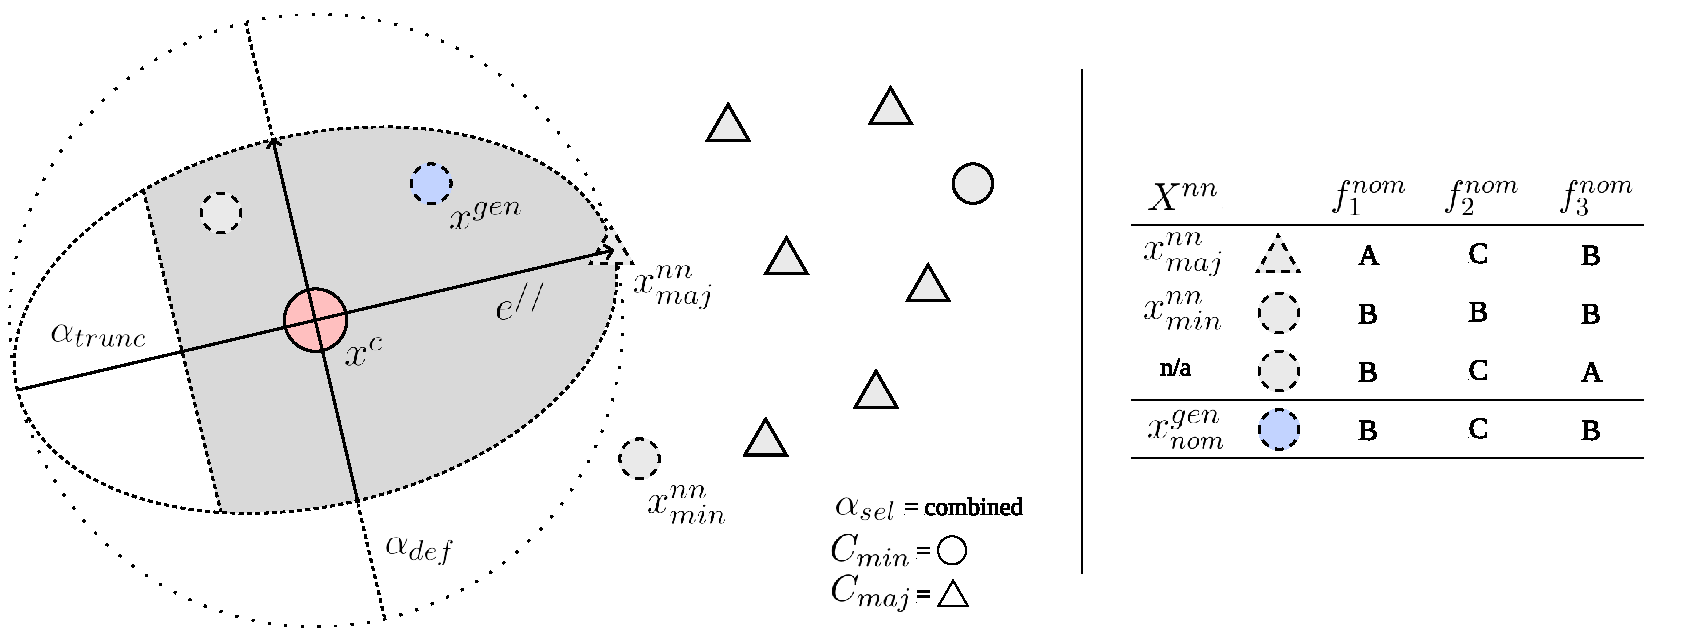
\includegraphics[width=\linewidth]{g-smote}
    \caption{A visual depiction of G-SMOTENC. In this example,
        $\alpha_{trunc}$ is approximately 0.5 and $\alpha_{def}$ is
        approximately 0.4.
    }~\label{fig:gsmote}
\end{figure}

\subsection{Selection Mechanism}

The data selection mechanism is preceded by the numerical encoding of the
nominal features. It combines the selection mechanisms of SMOTENC and
G-SMOTE, as shown in Algorithm~\ref{alg:selection}. The selection mechanism
inherits the minority, majority, and combined mechanisms proposed in G-SMOTE.
The nominal features in the minority and majority class observations,
$C_{maj}$ and $C_{min}$ are first encoded using a one-hot encoding approach
and replacing the constant 1 with the median of the standard deviations of the
continuous features in $C_{min}$ divided by 2. The nearest-neighbors
($X^{nn}$) of $x^c$ are determined based on $\alpha_{sel}$, which are passed
on to the generation mechanism to determine the nominal features' values of
$x^{gen}$ in the generation mechanism. Simultaneously, $x^{nn}$ is randomly
selected from $X^{nn}$ and will be used to generate $x^{gen}$'s continuous
features' values.


\begin{algorithm}
    \SetKwProg{Fn}{Function}{:}{end}
    \SetKwInput{KwGiven}{Given}
    \caption{G-SMOTENC's selection mechanism.}\label{alg:selection}
    \DontPrintSemicolon%
    
    % START
    \KwIn{$C_{maj}, C_{min}, \alpha_{sel}$}
    \KwOut{$x^c, x^{nn}$, $X^{nn}$}

    \Fn{CatEncoder($C_{maj}$, $C_{min}$)}{
        $S \leftarrow $ Standard deviations of the continuous features in $C_{min}$\\
        $\sigma_{med} \leftarrow median(S)$\\
        \ForAll{$i \in \{maj, min\}$}{
            \ForAll{$f \in C_i^T$}{
                \If{f is nominal}{
                    $f' \leftarrow OneHotEncode(f) \times \sigma_{med} / 2$ \\
                    $C_i' \leftarrow (C_i^T \setminus f)^T$\\
                    $C_i' \leftarrow (C_i'^T \cup f')^T$
                }
            }
        }
        \Return $C_{maj}'$, $C_{min}'$
    }

    \Fn{Surface($\alpha_{sel}$, $x^c$, $C_{maj}$, $C_{min}$)}{
        \If{$\alpha_{sel} = minority$}{
            $x^{nn} \in C_{min, k}$ 
            \tcp*[f]{One of the $k$-nearest neighbors of $x^c$ from
            $C_{min}$}\\
            $X^{nn} \leftarrow C_{min, k}$
        }
        \If{$\alpha_{sel} = majority$}{
            $x^{nn} \in C_{maj, 1}$ 
            \tcp*[f]{Nearest neighbor of $x^c$ from $C_{maj}$}\\
            $X^{nn} \leftarrow C_{maj, 1}$
        }
        \If{$\alpha_{sel}$ = combined}{
            $x^{nn}_{min} \in C_{min, k}$ \\
            $x^{nn}_{maj} \in C_{maj, 1}$ \\
            $x^{nn} \leftarrow argmin(||x^{nn}_{min}-x^c||,
            ||x^{nn}_{maj}-x^c||)$\\
            $X^{nn} \leftarrow C_{min, k} \cup C_{maj, 1}$
        }
        \Return $x^{nn}, X^{nn}$ \tcp*[f]{$X^{nn}$ is the set of $k$-nearest neighbors}\\
    }

    \Begin{
        $C_{maj}', C_{min}' \leftarrow CatEncoder(C_{maj}, C_{min})$ \\
        $x^c \in C_{min}'$ \tcp*[f]{Randomly select $x^c$ from $C_{min}'$}\\
        $x^{nn}, X^{nn} \leftarrow Surface(\alpha_{sel}, x^c, C_{maj}', C_{min}')$\\
        Reverse encoding of nominal features in $x^c$, $x^{nn}$ and $X^{nn}$
    }
\end{algorithm}

\subsection{Generation Mechanism}

G-SMOTENC's generation mechanism is shown in Algorithm~\ref{alg:generation}.
It divides the generation of $x^{gen}$ into two parts: (1) generation of
continuous feature values and (2) generation of nominal feature values.
First, the nominal features from $x^c$ and $x^{nn}$ are discarded. Afterward,
the continuous features are generated using G-SMOTE's generation mechanism;
within a hyper-spheroid defined with $\alpha_{trunc}$ and $\alpha_{def}$,
which allows the non-linear generation of synthetic observations between $x^c$
and $x^{nn}$. Finally, the nominal feature values are generated by the mode of
each feature within the observations in $X^{nn}$.

\begin{algorithm}
    \SetKwInput{KwGiven}{Given}
    \SetKwProg{Fn}{Function}{:}{end}
    \caption{G-SMOTENC's generation mechanism.}\label{alg:generation}
    \DontPrintSemicolon%

    % START
    \KwIn{$x^c, x^{nn}, X^{nn}, \alpha_{trunc}, \alpha_{def}$}
    \KwOut{$x^{gen}$}

    \Fn{Hyperball()}{
        $v_i \sim \mathcal{N}(0, 1)$\\
        $r \sim \mathcal{U}(0, 1)$\\
        $x^{gen} \leftarrow r^{1/p}\frac{(v_1, \ldots, v_p)}{||(v_1, \ldots,
        v_p)||}$\\
        \Return $x^{gen}$
    }

    \Fn{Vectors($x^c, x^{nn}, x^{gen}$)}{
        $e^{//} \leftarrow \frac{x^{nn}-x^c}{||x^{nn}-x^c||}$\\
        $x^{//} \leftarrow (x^{gen} \cdot e^{//})e^{//}$\\
        $x^{\perp} \leftarrow x^{gen} - x^{//}$\\
        \Return $x^{//}, x^{\perp}$
    }

    \Fn{Truncate($x^c, x^{nn}, x^{gen}, x^{//}, \alpha_{trunc}$)}{
        \If{$|\alpha_{trunc} - x^{//}| > 1$}{
            $x^{gen} \leftarrow x^{gen} - 2x^{//}$
        }
        \Return $x^{gen}$
    }

    \Fn{Deform($x^{gen}, x^{\perp}, \alpha_{def}$)}{
        \Return $x^{gen} - \alpha_{def}x^{\perp}$
    }

    \Fn{Translate($x^c, x^{gen}, R$)}{
        \Return $x^c + R x^{gen}$
    }

    \Fn{GenNominal($X^{nn}$)}{
        $x^{gen}_{nom} = \emptyset $\\
        \ForAll{$f \in (X^{nn})^T$}{
            \If{f is nominal}{
                $x^{gen}_{nom} \cup \{mode(f)\}$\tcp*[f]{Ties are decided with
                random selection}\\
            }
        }
        \Return $x^{gen}_{nom}$
    }

    \Begin{
        Discard nominal features from $x^c$ and $x^{nn}$\\
        $x^{gen} \leftarrow Hyperball()$\\
        $x^{//}, x^{\perp} \leftarrow Vectors(x^c, x^{nn}, x^{gen})$\\
        $x^{gen} \leftarrow Truncate(x^c, x^{nn}, x^{gen}, x^{//}, \alpha_{trunc})$\\
        $x^{gen} \leftarrow Deform(x^{gen}, x^{\perp}, \alpha_{def})$\\
        $x^{gen} \leftarrow Translate(x^c, x^{gen},
        ||x^{nn}_{cont}-x^c||)$\\
        $x^{gen}_{nom} \leftarrow GenNominal(X^{nn})$\\
        $x^{gen} \leftarrow x^{gen} \cup x^{gen}_{nom}$
    }

\end{algorithm}


\section{Methodology}~\label{sec:methodology-gsmotenc}

This section describes how the evaluation of G-SMOTENC was performed. We
describe the datasets used in the experiment, their source and preprocessing
steps executed in Section~\ref{sec:experimental_data-gsmotenc}. The resampling and
classification methods used to analyze G-SMOTE's performance are listed in
Section~\ref{sec:ml_algorithms-gsmotenc}. The performance metrics used are defined in
Section~\ref{sec:performance_metrics-gsmotenc}. Finally, the experimental procedure is
described in Section~\ref{sec:experimental_procedure-gsmotenc}.

\subsection{Experimental Data}~\label{sec:experimental_data-gsmotenc}

The datasets used in this experiment were extracted from the
\href{https://archive.ics.uci.edu}{UC Irvine Machine Learning Repository}. All
of the datasets are publicly available and cover a range of different domains.
The criteria to select the datasets ensured that all datasets are imbalanced
and contained non-metric features (\textit{i.e.}, ordinal, nominal or binary).
These datasets are used to show how the performance of different
classifiers varies across over/undersamplers.

All datasets were initially preprocessed manually with minimal manipulations.
We removed features and/or observations with missing values and identified the
non-metric features. The second stage of preprocessing was done
systematically. It starts with the generation of artificially imbalanced
datasets with different Imbalance Ratios ($IR=\frac{|C_{maj}|}{|C_{min}|}$).
For each original dataset, we create its more imbalanced versions at intervals
of 10, while ensuring that $|C_{min}| \ge 15$. The sampling strategy was
determined for class $n \in \{1,\ldots,n,\ldots,m\}$ as a linear interpolation
using $|C_{maj}|$ and $|C_{min}'|=\frac{|C_{maj}|}{IR_{new}}$, as shown in
equation~\ref{eq:sampling}.

\begin{equation}~\label{eq:sampling}
    |C_i|^{imb} =
    \min(\frac{|C_{min}'|-|C_{maj}|}{n-1}.|C_i|+|C_{max}|, |C_i|)
\end{equation}

The new, artificially imbalanced dataset, is formed by sampling observations
without replacement from each $C_i$ such that $C_i' \subseteq C_i , |C_i'| =
|C_i|^{imb}$. The artificially imbalanced datasets are marked with its
imbalance ratio as a suffix in Table~\ref{tbl:datasets_description}.

The datasets (both original and artificially imbalanced versions) are then
filtered to ensure all datasets have a minimum of 500 observations.  The
remaining datasets with a number of observations larger than 5000 are randomly
sampled to match this number of observations. Afterward, we remove target
classes with a frequency lower than 15 observations for each remaining
dataset. Finally, the continuous and discrete features are scaled to the range
$[0,1]$ to ensure a common range between all features. The description of the
resulting datasets is shown in Table~\ref{tbl:datasets_description}.

\begin{longtable}{cccccccc}
\caption[Description of the datasets collected after data preprocessing.]{Description of the datasets collected after data preprocessing. The sampling strategy is similar across datasets. Legend: (IR) Imbalance Ratio}
\label{tbl:datasets_description}\\
\toprule
           Dataset &  Metric &  Non-Metric &  Obs. &  Min. Obs. &  Maj. Obs. &     IR &  Classes \\
\midrule
\endfirsthead
\caption[]{Description of the datasets collected after data preprocessing. The sampling strategy is similar across datasets. Legend: (IR) Imbalance Ratio} \\
\toprule
           Dataset &  Metric &  Non-Metric &  Obs. &  Min. Obs. &  Maj. Obs. &     IR &  Classes \\
\midrule
\endhead
\midrule
\multicolumn{8}{r}{{Continued on next page}} \\
\midrule
\endfoot

\bottomrule
\endlastfoot
           Abalone &       1 &           7 &  4139 &         15 &        689 &  45.93 &       18 \\
             Adult &       8 &           6 &  5000 &       1268 &       3732 &   2.94 &        2 \\
        Adult (10) &       8 &           6 &  5000 &        451 &       4549 &  10.09 &        2 \\
         Annealing &       4 &           6 &   790 &         34 &        608 &  17.88 &        4 \\
            Census &      24 &           7 &  5000 &        337 &       4663 &  13.84 &        2 \\
     Contraceptive &       4 &           5 &  1473 &        333 &        629 &   1.89 &        3 \\
Contraceptive (10) &       4 &           5 &  1036 &         62 &        629 &  10.15 &        3 \\
Contraceptive (20) &       4 &           5 &   990 &         31 &        629 &  20.29 &        3 \\
Contraceptive (31) &       4 &           5 &   973 &         20 &        629 &  31.45 &        3 \\
Contraceptive (41) &       4 &           5 &   966 &         15 &        629 &  41.93 &        3 \\
         Covertype &       2 &          10 &  5000 &         20 &       2449 & 122.45 &        7 \\
   Credit Approval &       9 &           6 &   653 &        296 &        357 &   1.21 &        2 \\
     German Credit &      13 &           7 &  1000 &        300 &        700 &   2.33 &        2 \\
German Credit (10) &      13 &           7 &   770 &         70 &        700 &  10.00 &        2 \\
German Credit (20) &      13 &           7 &   735 &         35 &        700 &  20.00 &        2 \\
German Credit (30) &      13 &           7 &   723 &         23 &        700 &  30.43 &        2 \\
German Credit (41) &      13 &           7 &   717 &         17 &        700 &  41.18 &        2 \\
     Heart Disease &       5 &           5 &   740 &         22 &        357 &  16.23 &        5 \\
Heart Disease (21) &       5 &           5 &   735 &         17 &        357 &  21.00 &        5 \\
\end{longtable}


\subsection{Machine Learning Algorithms}~\label{sec:ml_algorithms-gsmotenc}

The choice of classifiers used in the experimental procedure was based on
their type (tree-based, nearest neighbors-based, linear model and
ensemble-based), popularity and consistency in performance. We used Decision
Tree (DT), a K-Nearest Neighbors (KNN) classifier, a Logistic
Regression (LR) and a Random Forest (RF).

Given the lack of existing oversamplers that address imbalanced learning
problems with mixed data types, the amount of benchmark methods used is also
limited. We used three appropriate, well-known methods and one state-of-the-art
oversampling method: SMOTENC, RUS, ROS and SMOTE-ENC\@. Table~\ref{tbl:grid}
shows the hyperparameters used for the parameter search described in
Section~\ref{sec:experimental_procedure-gsmotenc}.

\begin{table}[ht]
	\centering
    \caption{\label{tbl:grid}
        Hyperparameter definition for the classifiers and resamplers used in
        the experiment.
    }
	\begin{tabular}{lll}
		\toprule
		Classifier      & Hyperparameter                   & Values                         \\
		\midrule
        DT              & min.\ samples split              & 2                              \\
                        & criterion                        & gini                           \\
                        & max depth                        & 3, 6                           \\
		LR              & maximum iterations               & 10000                          \\
                        & multi-class                      & One-vs-All                     \\
		                & solver                           & saga                           \\
                        & penalty                          & None, L1, L2                   \\
		KNN             & \# neighbors                     & 3, 5                           \\
                        & weights                          & uniform                        \\
                        & metric                           & euclidean                      \\
		RF              & min.\ samples split              & 2                              \\
		                & \# estimators                    & 50, 100                        \\
		                & Max depth                        & 3, 6                           \\
                        & criterion                        & gini                           \\
		\toprule
		Resampler       &                                  &                                \\
		\midrule
		SMOTENC         & \# neighbors                     & 3, 5                           \\
		SMOTE-ENC       & \# neighbors                     & 3, 5                           \\
		G-SMOTENC       & \# neighbors                     & 3, 5                           \\
                        & deformation factor               & 0.0, 0.25, 0.5, 0.75, 1.0      \\
                        & truncation factor                & -1.0, -0.5, 0.0, 0.5, 1.0      \\
                        & selection strategy               & ``combined'',
                        ``minority'', ``majority''\\
		RUS             & replacement                      & False                          \\
		ROS             & (no applicable parameters)       &                                \\
		\bottomrule
	\end{tabular}
\end{table}

\subsection{Performance Metrics}~\label{sec:performance_metrics-gsmotenc}

The choice of the performance metric plays a critical role in assessing
the effect on classification tasks. The typical performance metrics,
\textit{e.g.}, Overall Accuracy (OA), are intuitive to interpret but are often
inappropriate to measure a classifier's performance in an imbalanced learning
context~\cite{sun2009classification}. For example, to estimate an event that
occurs in 1\% of the dataset, a constant classifier would obtain an OA of 0.99
and still be unusable. However, this metric is still reported in some of our
results to maintain interpretability.

Recent surveys consider Geometric-mean (G-mean), F1-score
(F-score), $Sensitivity = \frac{TP}{FN+TP}$ and $Specificity = \frac{TN}{TN +
FP}$ appropriate and common performance metrics in imbalanced learning
contexts~\cite{rout2018handling, Jeni2013,
japkowicz2013assessment}. G-mean and F-score are defined
equations~\ref{eq:gmean} and~\ref{eq:fscore}, respectively.

\begin{equation}~\label{eq:gmean}
    \ensuremath{\textit{G-mean}} = \sqrt{\overline{Sensitivity} \times
    \overline{Specificity}}
\end{equation}

\begin{equation}~\label{eq:fscore}
    \ensuremath{\textit{F-score}} = 2\times\frac{\overline{Precision} \times
    \overline{Recall}}{\overline{Precision} + \overline{Recall}}
\end{equation}

They are calculated as a function of the number of False/True Positives (FP
and TP) and False/True Negatives (FN and TN), with $Precision =
\frac{TP}{TP+FP}$ and $Recall = \frac{TP}{TP+FN}$. This led us to use, along
with OA, both F-score and G-mean as the main performance metrics for this
study. 

\subsection{Experimental Procedure}~\label{sec:experimental_procedure-gsmotenc}

The experimental procedure was applied similarly to all combinations of
resamplers, classifiers and hyperparameter combinations across all datasets.
The evaluation of the models' performance was tested using a 5-fold
Cross-Validation (CV) approach. The mean performance in the test set is
calculated over the five folds and three different runs of the experimental
procedure for each combination of resampling/classifier hyperparameters. For
each dataset, we select the results of the hyperparameters that optimize the
performance of a resampler/classifier.
Figure~\ref{fig:experimental_procedure-gsmotenc}
shows a diagram of the experimental procedure described.

\begin{figure}
	\centering
	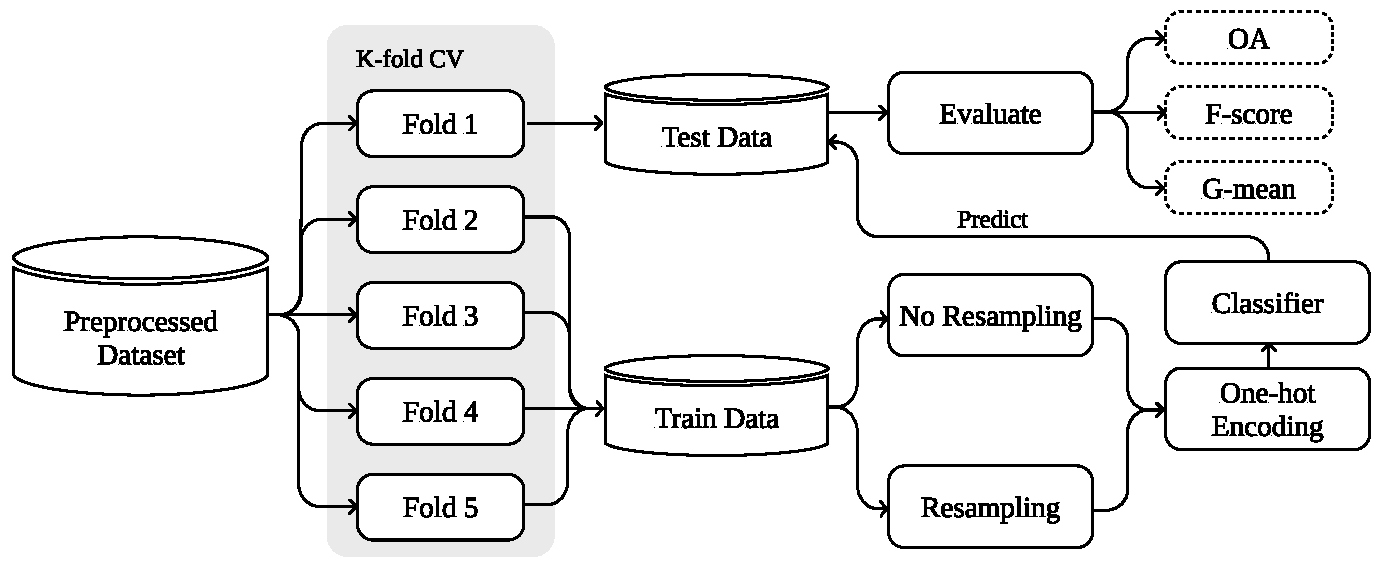
\includegraphics[width=.8\linewidth]{experimental_procedure}
    \caption{Experimental procedure used in this study.
    }~\label{fig:experimental_procedure-gsmotenc}
\end{figure}

A CV run consists of a stratified partitioning (\textit{i.e.}, each partition
contains the same relative frequencies of target labels) of the dataset into
five parts. A given resampler/classifier combination with a specific set of
hyperparameters is fit and tested five times, using one of the partitions as a
test set and the remaining ones as the training set. In the ML pipeline
defined for each run, the nominal features are one-hot encoded after
oversampling and before passing the data to the classifier. The estimated
performance consists of the average classification performance across the five
tests and three runs (\textit{i.e.}, a total of 15 tests). 

\subsection{Software Implementation}~\label{sec:software_implementation-gsmotenc}

The algorithmic implementation of G-SMOTENC was written using the Python
programming language and is available in the open-source package
\href{https://github.com/joaopfonseca/ml-research}{ML-Research}~\cite{Fonseca2021al},
along with other utilities used to produce the experiment and outputs used in
Section~\ref{sec:results_and_discussion-gsmotenc}. In addition, the packages
\href{https://github.com/scikit-learn/scikit-learn/}{Scikit-Learn}~\cite{Pedregosa2011},
\href{https://github.com/scikit-learn-contrib/imbalanced-learn}{Imbalanced-Learn}~\cite{JMLR:v18:16-365}
and \href{https://github.com/georgedouzas/research-learn/}{Research-Learn}
were also used in the experimental procedure to get the implementations of the
classifiers, benchmark over/undersamplers and run the experimental procedure.
The original SMOTE-ENC implementation was retrieved from the
\href{https://github.com/Mimimkh/SMOTE-ENC-code}{authors' GitHub repository}.
The Latex code, Python scripts (including data pulling and preprocessing,
experiment setup and analysis of results), as well as the datasets used, are
available in this \href{https://github.com/joaopfonseca/publications}{GitHub
repository}.
 
\section{Results and Discussion}~\label{sec:results_and_discussion-gsmotenc}

In this section, we present the experimental results. We focus on the
comparison of classification performance using oversamplers whose generation
mechanism is compatible with datasets containing both nominal and continuous
features. The experimental results were analyzed in two stages: (1) in
Section~\ref{sec:results-gsmotenc} we analyze mean rankings and absolute performances
and in Section~\ref{sec:statistical_analysis-gsmotenc} we show the results of our
statistical analysis. Section~\ref{sec:discussion-gsmotenc} discusses the main
insights extracted by analyzing the experimental results.

\subsection{Results}~\label{sec:results-gsmotenc}

Table~\ref{tbl:mean_sem_ranks} presents the mean rankings of CV scores between
the different combinations of oversamplers, metrics and classifiers. These
results were calculated by assigning a ranking score for each oversampler from
1 (best) to 4 (worst) for each dataset, metric and classifier.

\begingroup\small
{\setlength{\tabcolsep}{5pt}
\begin{longtable}{cccccccc}
\caption{Mean rankings over the different datasets, folds and runs used in the experiment.}
\label{tbl:mean_sem_ranks}\\
\toprule
Classifier &  Metric &                G-SMOTENC &                     NONE &         SMOTENC &                      ROS &             RUS &       SMOTE-ENC \\
\midrule
\endfirsthead
\caption[]{Mean rankings over the different datasets, folds and runs used in the experiment.} \\
\toprule
Classifier &  Metric &                G-SMOTENC &                     NONE &         SMOTENC &                      ROS &             RUS &       SMOTE-ENC \\
\midrule
\endhead
\midrule
\multicolumn{8}{r}{{Continued on next page}} \\
\midrule
\endfoot

\bottomrule
\endlastfoot
        DT &      OA &          1.66 $\pm$ 0.13 & \textbf{1.61 $\pm$ 0.27} & 3.58 $\pm$ 0.20 &          4.68 $\pm$ 0.15 & 5.42 $\pm$ 0.27 & 4.05 $\pm$ 0.23 \\
        DT & F-Score & \textbf{1.32 $\pm$ 0.11} &          3.84 $\pm$ 0.40 & 3.13 $\pm$ 0.20 &          4.32 $\pm$ 0.19 & 5.47 $\pm$ 0.23 & 2.92 $\pm$ 0.34 \\
        DT &  G-Mean & \textbf{1.68 $\pm$ 0.24} &          5.84 $\pm$ 0.09 & 2.82 $\pm$ 0.21 &          2.95 $\pm$ 0.32 & 4.26 $\pm$ 0.32 & 3.45 $\pm$ 0.30 \\
       KNN &      OA &          2.50 $\pm$ 0.17 & \textbf{1.37 $\pm$ 0.28} & 4.21 $\pm$ 0.25 &          3.34 $\pm$ 0.35 & 5.68 $\pm$ 0.22 & 3.89 $\pm$ 0.15 \\
       KNN & F-Score & \textbf{1.37 $\pm$ 0.16} &          3.95 $\pm$ 0.35 & 3.11 $\pm$ 0.29 &          3.47 $\pm$ 0.36 & 5.53 $\pm$ 0.23 & 3.58 $\pm$ 0.23 \\
       KNN &  G-Mean & \textbf{1.74 $\pm$ 0.17} &          5.84 $\pm$ 0.12 & 2.89 $\pm$ 0.23 &          3.76 $\pm$ 0.33 & 3.00 $\pm$ 0.45 & 3.76 $\pm$ 0.23 \\
        LR &      OA &          2.74 $\pm$ 0.19 & \textbf{1.37 $\pm$ 0.28} & 3.08 $\pm$ 0.21 &          4.34 $\pm$ 0.30 & 5.74 $\pm$ 0.17 & 3.74 $\pm$ 0.28 \\
        LR & F-Score & \textbf{2.11 $\pm$ 0.24} &          4.53 $\pm$ 0.35 & 2.37 $\pm$ 0.28 &          3.47 $\pm$ 0.32 & 5.21 $\pm$ 0.27 & 3.32 $\pm$ 0.38 \\
        LR &  G-Mean &          2.13 $\pm$ 0.26 &          6.00 $\pm$ 0.00 & 3.61 $\pm$ 0.21 & \textbf{2.11 $\pm$ 0.23} & 3.32 $\pm$ 0.40 & 3.84 $\pm$ 0.28 \\
        RF &      OA &          1.82 $\pm$ 0.11 & \textbf{1.24 $\pm$ 0.09} & 3.97 $\pm$ 0.16 &          4.32 $\pm$ 0.21 & 5.92 $\pm$ 0.06 & 3.74 $\pm$ 0.22 \\
        RF & F-Score & \textbf{1.32 $\pm$ 0.13} &          5.05 $\pm$ 0.31 & 3.16 $\pm$ 0.22 &          3.05 $\pm$ 0.31 & 5.37 $\pm$ 0.14 & 3.05 $\pm$ 0.27 \\
        RF &  G-Mean & \textbf{1.68 $\pm$ 0.22} &          5.79 $\pm$ 0.21 & 3.26 $\pm$ 0.28 &          2.47 $\pm$ 0.30 & 3.89 $\pm$ 0.35 & 3.89 $\pm$ 0.19 \\
\end{longtable}

}
\endgroup

Table~\ref{tbl:mean_sem_scores} presents the mean CV scores. Except for the
OA metric, G-SMOTENC either outperformed or matched the remaining
oversamplers.

\begingroup\small
{\setlength{\tabcolsep}{4.8pt}
\begin{longtable}{cccccccc}
\caption{Mean scores over the different datasets, folds and runs used in the experiment}
\label{tbl:mean_sem_scores}\\
\toprule
Classifier &  Metric &                G-SMOTENC &                     NONE &                  SMOTENC &                      ROS &             RUS &       SMOTE-ENC \\
\midrule
\endfirsthead
\caption[]{Mean scores over the different datasets, folds and runs used in the experiment} \\
\toprule
Classifier &  Metric &                G-SMOTENC &                     NONE &                  SMOTENC &                      ROS &             RUS &       SMOTE-ENC \\
\midrule
\endhead
\midrule
\multicolumn{8}{r}{{Continued on next page}} \\
\midrule
\endfoot

\bottomrule
\endlastfoot
        DT &      OA &          0.74 $\pm$ 0.05 & \textbf{0.75 $\pm$ 0.04} &          0.68 $\pm$ 0.04 &          0.66 $\pm$ 0.04 & 0.58 $\pm$ 0.04 & 0.65 $\pm$ 0.04 \\
        DT & F-Score & \textbf{0.56 $\pm$ 0.04} &          0.52 $\pm$ 0.04 &          0.54 $\pm$ 0.04 &          0.52 $\pm$ 0.04 & 0.48 $\pm$ 0.04 & 0.51 $\pm$ 0.04 \\
        DT &  G-Mean & \textbf{0.69 $\pm$ 0.03} &          0.60 $\pm$ 0.02 &          0.68 $\pm$ 0.03 &          0.67 $\pm$ 0.03 & 0.65 $\pm$ 0.03 & 0.66 $\pm$ 0.03 \\
       KNN &      OA &          0.69 $\pm$ 0.04 & \textbf{0.73 $\pm$ 0.05} &          0.67 $\pm$ 0.04 &          0.69 $\pm$ 0.05 & 0.57 $\pm$ 0.04 & 0.68 $\pm$ 0.05 \\
       KNN & F-Score & \textbf{0.53 $\pm$ 0.04} &          0.50 $\pm$ 0.04 &          0.52 $\pm$ 0.04 &          0.52 $\pm$ 0.04 & 0.46 $\pm$ 0.04 & 0.51 $\pm$ 0.04 \\
       KNN &  G-Mean & \textbf{0.66 $\pm$ 0.03} &          0.58 $\pm$ 0.03 &          0.64 $\pm$ 0.03 &          0.62 $\pm$ 0.03 & 0.65 $\pm$ 0.03 & 0.63 $\pm$ 0.03 \\
        LR &      OA &          0.68 $\pm$ 0.05 & \textbf{0.75 $\pm$ 0.04} &          0.68 $\pm$ 0.05 &          0.66 $\pm$ 0.05 & 0.58 $\pm$ 0.04 & 0.67 $\pm$ 0.04 \\
        LR & F-Score & \textbf{0.54 $\pm$ 0.04} &          0.52 $\pm$ 0.04 & \textbf{0.54 $\pm$ 0.04} &          0.53 $\pm$ 0.04 & 0.48 $\pm$ 0.04 & 0.52 $\pm$ 0.04 \\
        LR &  G-Mean & \textbf{0.69 $\pm$ 0.02} &          0.60 $\pm$ 0.03 &          0.68 $\pm$ 0.02 & \textbf{0.69 $\pm$ 0.03} & 0.67 $\pm$ 0.03 & 0.67 $\pm$ 0.03 \\
        RF &      OA &          0.74 $\pm$ 0.04 & \textbf{0.76 $\pm$ 0.04} &          0.69 $\pm$ 0.04 &          0.69 $\pm$ 0.04 & 0.59 $\pm$ 0.04 & 0.68 $\pm$ 0.05 \\
        RF & F-Score & \textbf{0.57 $\pm$ 0.04} &          0.48 $\pm$ 0.04 &          0.55 $\pm$ 0.04 &          0.55 $\pm$ 0.04 & 0.49 $\pm$ 0.04 & 0.53 $\pm$ 0.04 \\
        RF &  G-Mean & \textbf{0.70 $\pm$ 0.02} &          0.57 $\pm$ 0.02 &          0.68 $\pm$ 0.03 &          0.69 $\pm$ 0.03 & 0.68 $\pm$ 0.03 & 0.68 $\pm$ 0.02 \\
\end{longtable}

}
\endgroup

\subsection{Statistical Analysis}~\label{sec:statistical_analysis-gsmotenc}

It is necessary to use methods that account for the multiple comparison
problem to conduct an appropriate statistical analysis in an experiment with
multiple datasets. Based on the recommendations found in~\cite{Demsar2006}, we
applied a Friedman test followed by a Holm-Bonferroni test for post-hoc
analysis.

In Section~\ref{sec:performance_metrics-gsmotenc} we explained that OA, although easily
interpretable, is not an appropriate performance metric for imbalanced
learning problems. Therefore, the statistical analysis was developed using the
two imbalance-appropriate metrics used in the study: F-Score and G-Mean. Based
on the Friedman test~\cite{Friedman1937}, there is a statistically
significant difference in performance across resampling methods. The results
of this test are shown in Table~\ref{tbl:friedman_test}. The null hypothesis
is rejected in all cases.

\begin{longtable}{cccc}
\caption{Results for the Friedman test. Statistical significance is tested at a level of $\alpha = 0.05$. The null hypothesis is that there is no difference in the classification outcome across resamplers.}
\label{tbl:friedman_test}\\
\toprule
Classifier &  Metric & p-value &  Significance \\
\midrule
\endfirsthead
\caption[]{Results for the Friedman test. Statistical significance is tested at a level of $\alpha = 0.05$. The null hypothesis is that there is no difference in the classification outcome across resamplers.} \\
\toprule
Classifier &  Metric & p-value &  Significance \\
\midrule
\endhead
\midrule
\multicolumn{4}{r}{{Continued on next page}} \\
\midrule
\endfoot

\bottomrule
\endlastfoot
        DT & F-Score & 2.2e-10 &          True \\
        DT &  G-Mean & 1.2e-10 &          True \\
       KNN & F-Score & 2.3e-09 &          True \\
       KNN &  G-Mean & 9.4e-10 &          True \\
        LR & F-Score & 2.1e-07 &          True \\
        LR &  G-Mean & 9.7e-11 &          True \\
        RF & F-Score & 8.5e-12 &          True \\
        RF &  G-Mean & 2.0e-10 &          True \\
\end{longtable}


We performed a Holm-Bonferroni test to understand whether the difference in
the performance of G-SMOTENC is statistically significant to the remaining
resampling methods. The results of this test are shown in
Table~\ref{tbl:holms_test}. The null hypothesis is rejected in 33 out of 40
trials.

\begin{longtable}{ccccccc}
\caption{Adjusted p-values using the Holm-Bonferroni test. Statistical significance is tested at a level of $\alpha = 0.05$. The null hypothesis is that the benchmark methods perform similarly to the control method (G-SMOTENC).}
\label{tbl:holms_test}\\
\toprule
Classifier &  Metric &               NONE &            SMOTENC &                ROS &                RUS &          SMOTE-ENC \\
\midrule
\endfirsthead
\caption[]{Adjusted p-values using the Holm-Bonferroni test. Statistical significance is tested at a level of $\alpha = 0.05$. The null hypothesis is that the benchmark methods perform similarly to the control method (G-SMOTENC).} \\
\toprule
Classifier &  Metric &               NONE &            SMOTENC &                ROS &                RUS &          SMOTE-ENC \\
\midrule
\endhead
\midrule
\multicolumn{7}{r}{{Continued on next page}} \\
\midrule
\endfoot

\bottomrule
\endlastfoot
        DT & F-Score & \textbf{{1.5e-04}} & \textbf{{1.5e-04}} & \textbf{{7.3e-06}} & \textbf{{1.2e-06}} &          {1.0e-01} \\
        DT &  G-Mean & \textbf{{5.6e-07}} & \textbf{{2.7e-03}} & \textbf{{2.8e-02}} & \textbf{{3.9e-04}} & \textbf{{2.3e-02}} \\
       KNN & F-Score & \textbf{{6.4e-04}} & \textbf{{2.2e-04}} & \textbf{{7.2e-04}} & \textbf{{6.4e-04}} & \textbf{{5.9e-06}} \\
       KNN &  G-Mean & \textbf{{1.6e-05}} & \textbf{{9.6e-03}} & \textbf{{6.5e-03}} &          {2.0e-01} & \textbf{{3.5e-03}} \\
        LR & F-Score & \textbf{{4.0e-03}} &          {6.1e-01} & \textbf{{9.2e-03}} & \textbf{{3.6e-04}} &          {5.6e-02} \\
        LR &  G-Mean & \textbf{{1.6e-07}} & \textbf{{4.0e-04}} &          {8.6e-01} &          {2.4e-01} & \textbf{{4.7e-03}} \\
        RF & F-Score & \textbf{{1.7e-06}} & \textbf{{2.4e-04}} & \textbf{{8.0e-03}} & \textbf{{1.7e-06}} & \textbf{{8.0e-03}} \\
        RF &  G-Mean & \textbf{{3.8e-06}} & \textbf{{8.8e-03}} &          {2.5e-01} & \textbf{{2.3e-02}} & \textbf{{1.7e-03}} \\
\end{longtable}


\subsection{Discussion}~\label{sec:discussion-gsmotenc}

The results reported in Section~\ref{sec:results-gsmotenc} show that G-SMOTENC
consistently outperforms the remaining oversampling approaches. Based on the
two metrics appropriate for imbalanced learning problems, G-Mean and F-Score,
in the average rankings shown in Table~\ref{tbl:mean_sem_ranks} G-SMOTENC was
only outperformed once by a small margin. Unlike the results reported
in~\cite{mukherjee2021smote}, SMOTE-ENC's performance was rarely superior to
SMOTENC's.

The relative difference in the classifiers' performance is better visible in
Table~\ref{tbl:mean_sem_scores}. Using an RF classifier, for example, the
impact of using G-SMOTENC compared to no oversampling improves, on average, 13
percentual points on G-mean and nine percentual points using F-Score. 

The difference in performance between oversamplers was found to be
statistically significant across classifiers and performance metrics in the
Friedman test. The p-values of this test are reported in
Table~\ref{tbl:friedman_test}. The superiority of G-SMOTENC was confirmed with
the results from the Holm-Bonferroni test shown in Table~\ref{tbl:holms_test}.
This test showed that G-SMOTENC outperformed with statistical significance the
remaining resamplers in 82.5\% of the comparisons done.

\begin{figure}[ht]
	\centering
	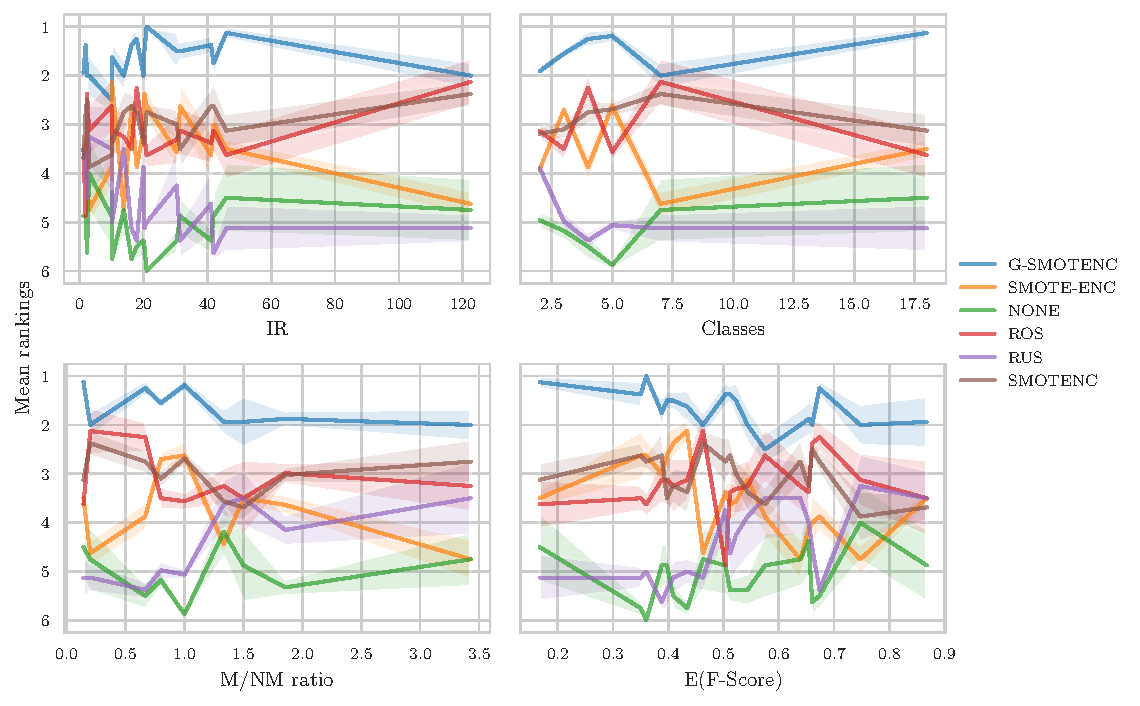
\includegraphics[width=\linewidth]{consistency_analysis_plot}
    \caption{Average ranking of oversamplers over different characteristics of
        the datasets used in the experiment. Legend: IR --- Imbalance Ratio,
        Classes --- Number of classes in the dataset, M/NM ratio --- ratio
        between the number of metric and non-metric features, E$($F-Score$)$
        --- Mean F-Score of dataset across all combinations of classifiers and
        oversamplers.
    }~\label{fig:consistency_analysis}
\end{figure}


The results from this experiment expose some well-known limitations of SMOTE,
which become particularly evident with SMOTENC. Specifically, the lack of
diversity in the generated data and, on some occasions, the near-duplication
of observations discussed in~\cite{Douzas2019} may be a possible
explanation for the performance of SMOTENC being comparable to ROS'
performance, visible in Figure~\ref{fig:consistency_analysis}. In this
figure, three groups of resampling methods with comparable performance are
visible: (1) G-SMOTENC, the top-performing method, (2) SMOTENC, ROS and
SMOTE-ENC, where SMOTE-ENC has the most inconsistent behavior and (3) RUS and
no oversampling, the worst-performing approaches. In addition, G-SMOTENC's
superiority seems invariable to the dataset's characteristics, with little
overlap with the remaining benchmark methods.

\section{Conclusion}~\label{sec:conclusion-gsmotenc}

This paper presented G-SMOTENC, a new oversampling algorithm that combines
G-SMOTE and SMOTENC. This oversampling algorithm leverages G-SMOTE's data
selection and generation mechanisms into datasets with mixed data types. This
was achieved by encoding and generating nominal feature values using SMOTENC's
approach. The quality of the data generated with G-SMOTENC was tested over 20
datasets with different imbalance ratios, metric/non-metric feature ratios
and number of classes. These results were compared to no oversampling,
SMOTENC, Random Oversampling, Random Undersampling and SMOTE-ENC using a
Decision Tree, K-Nearest Neighbors, Logistic Regression and Random Forest as
classifiers.

G-SMOTENC can be seen as a drop-in replacement of SMOTENC, since when
$\alpha_{trunc}=1$, $\alpha_{def}=1$ and $\alpha_{sel}=minority$, SMOTENC is
reproduced. G-SMOTENC has three additional hyperparameters that allow for
greater customization of the selection and generation mechanisms.  However,
determining the optimal parameters a priori (\textit{i.e.}, with reduced
parameter tuning) is a topic for future work.

The results show that G-SMOTENC performs significantly better when compared to
its more popular counterparts (SMOTENC, Random Oversampling and Random
Undersampling), as well as a recently proposed oversampling algorithm for
mixed data types (SMOTE-ENC). This performance improvement is related to
G-SMOTENC's selection mechanism, which finds a safer region for data
generation, along with its generation mechanism which increases the diversity
of the generated observations compared to SMOTENC. The G-SMOTENC
implementation used in this study is available in the
\href{https://github.com/joaopfonseca/ml-research}{open-source Python library
``ML-Research''} and is fully compatible with the Scikit-Learn ecosystem.

\chapter{%
    Improving Imbalanced Land Cover Classification with K-means SMOTE\@:
    Detecting and Oversampling Distinctive Minority Spectral Signatures
}~\label{chp:kmeans-smote}


\graphicspath{{figures/kmeans-smote-lulc/}}

\begin{adjustwidth}{30pt}{30pt}

    Land cover maps are a critical tool to support informed policy
    development, planning, and resource management decisions. With significant
    upsides, the automatic production of Land Use/Land Cover maps has been a
    topic of interest for the remote sensing community for several years, but
    it is still fraught with technical challenges. One such challenge is the
    imbalanced nature of most remotely sensed data. The asymmetric class
    distribution impacts negatively the performance of classifiers and adds a
    new source of error to the production of these maps. In this paper, we
    address the imbalanced learning problem, by using K-means and the
    Synthetic Minority Oversampling TEchnique (SMOTE) as an improved
    oversampling algorithm.  K-Means SMOTE improves the quality of newly
    created artificial data by addressing both the between-class imbalance, as
    traditional oversamplers do, but also the within-class imbalance, avoiding
    the generation of noisy data while effectively overcoming data imbalance.
    The performance of K-means SMOTE is compared to three popular oversampling
    methods (Random Oversampling, SMOTE and Borderline-SMOTE) using seven
    remote sensing benchmark datasets, three classifiers (Logistic Regression,
    K-Nearest Neighbors and Random Forest Classifier) and three evaluation
    metrics using a 5-fold cross-validation approach with 3 different
    initialization seeds. The statistical analysis of the results show that
    the proposed method consistently outperforms the remaining oversamplers
    producing higher quality land cover classifications. These results suggest
    that LULC data can benefit significantly from the use of more
    sophisticated oversamplers as spectral signatures for the same class can
    vary according to geographical distribution.

\end{adjustwidth}

\vspace{.5cm}
\textbf{Keywords:} LULC Classification; Imbalanced Learning; Oversampling;
Data Augmentation; Clustering

\section{Introduction}

The increasing amount of remote sensing missions granted the access to dense
time series (TS) data at a global level and provides up-to-date, accurate land
cover information \cite{Drusch2012}. This information is often materialized
through Land Use and Land Cover (LULC) maps. While Land Cover maps
define the biophysical cover found on the surface of the earth, Land Use maps
define how it is used by humans \cite{Fritz2017}. Both Land Use and Land Cover
maps constitute an essential asset for various purposes, such as land cover
change detection, urban planning, environmental monitoring and natural hazard
assessment \cite{Khatami2016}. However, the timely production of accurate and
updated LULC maps is still a challenge within the remote sensing community
\cite{Wulder2018}. LULC maps are produced based on two main approaches:
photo-interpreted by the human eye, or automatic mapping using remotely sensed
data and classification algorithms.

While photo-interpreted LULC maps rely on human operators and can be more
reliable, they also present some significant disadvantages. The most important
disadvantage is the cost of production, in fact photo-interpretation consumes
significant resources, both in terms of money and time. Because of that, they
are not frequently updated and not suitable for operational mapping over large
areas.  Finally, there is also the issue of overlooking rare or small-area
classes, due to factors such as the minimum mapping unit being used.

Automatic mapping with classification algorithms based on machine-learning
(ML) have been extensively researched and used to speed up and reduce the
costs of the production process \cite{Khatami2016, Gavade2019,
Kaur2019}. Improvements in classification algorithms are sure to have
significant impact in the efficiency with which remote sensing imagery is
used. Several challenges have been identified in order to improve automatic
classification:

\begin{enumerate}
    \item Improve the ability to handle high-dimensional datasets, in cases
        such as Multi-spectral TS composites high-dimensionality increases the
        complexity of the problem and creates a strain on computational power
        \cite{Stromann2020}.
    \item Improve class separability, as the production of an accurate LULC map
        can be hindered by the existence of classes with similar spectral
        signatures, making these classes difficult to distinguish
        \cite{Alonso-Sarria2019}.
    \item Resilience to mislabelled LULC patches, as the use of
        photo-interpreted training data poses a threat to the quality of any
        LULC map produced with this strategy, since factors such as the minimum
        mapping unit tend to cause the overlooking of small-area LULC patches
        and generates noisy training data that may reduce the prediction
        accuracy of a classifier \cite{Pelletier2017}.
    \item Dealing with rare land cover classes, due to the varying levels of
        area coverage for each class. In this case using a purely random
        sampling strategy will amount to a dataset with a roughly proportional
        class distribution as the one on the multi/hyperspectral
        image. On the other hand, the acquisition of training
        datasets containing balanced class frequencies is often unfeasible.
        This causes an asymmetry in class distribution, where some classes are
        frequent in the training dataset, while others have little expression
        \cite{Wang2019, Feng2019}.
\end{enumerate}

The latter challenge is known, in machine learning, as the imbalanced learning
problem \cite{Chawla2004}. It is defined as a skewed distribution of instances
found in a dataset among classes in both binary and multi-class problems
\cite{Abdi2016}. This asymmetry in class distribution negatively impacts the
performance of classifiers, especially in multi-class problems.  The problem
comes from the fact that during the learning phase, classifiers are optimized
to maximize an objective function, with overall accuracy being the most common
one \cite{Maxwell2018}. This means that instances belonging to minority
classes contribute less to the optimization process, translating into a bias
towards majority classes. As an example, a trivial classifier can achieve 99\%
overall accuracy on a binary dataset where 1\% of the instances belong to the
minority class if it classifies all instances as belonging to the majority
class. This is an especially significant issue in the automatic classification
of LULC maps, as the distribution of the different land-use classes tends to
be highly imbalanced.  Therefore, improvements in the ability to deal with
imbalanced datasets will translate into important progress in the automatic
classification of LULC maps.

There are three different types of approaches to deal with the class imbalance
problem \cite{Fernandez2013,Kaur2019}:

\begin{enumerate}
    \item Cost-sensitive solutions. Introduces a cost matrix to the learning
        phase with misclassification costs attributed to each class. Minority
        classes will have a higher cost than majority classes, forcing the
        algorithm to be more flexible and adapt better to predict minority
        classes.
    \item Algorithmic level solutions. Specific classifiers are modified to
        reinforce the learning on minority classes. Consists on the creation or
        adaptation of classifiers.
    \item Resampling solutions. Rebalances the dataset's class distribution by
        removing majority class instances and/or generating artificial minority
        instances. This can be seen as an external approach, where the
        intervention occurs before the learning phase, benefitting from
        versatility and independency from the classifier used.
\end{enumerate}

Since resampling strategies represent a set of methods that are detached from
classifiers by operating at the data level, they allow the use of any off the
shelf algorithm, without the need for any type of changes or adaptions to the
algorithm. Specifically, in the case of oversampling (defined below), the user
is able to balance the dataset's class distribution by without the loss of
information, which is not the case with undersampling techniques. This is a
significant advantage especially considering that most users in remote sensing
are not expert machine learning engineers. 

Within resampling approaches there are three subgroups of approaches
\cite{Fernandez2013,Kaur2019,Luengo2020}:

\begin{enumerate}
    \item Undersampling methods, which rebalance class distribution by removing
        instances from the majority classes.
    \item Oversampling methods, which rebalance datasets by generating new
        artificial instances belonging to the minority classes.
    \item Hybrid methods, which are a combination of both oversampling and
        undersampling, resulting in the removal of instances in the majority
        classes and the generation of artificial instances in the minority
        classes.
\end{enumerate}

Resampling methods can be further distinguished between non-informed and
heuristic (i.e., informed) resampling techniques
\cite{Fernandez2013,Luengo2020,Garcia2016}. The former consist of methods that
duplicate/remove a random selection of data points to set class distributions
to user-specified levels, and are therefore a simpler approach to the problem.
The latter consists of more sophisticated approaches that aim to perform
over/undersampling based on the points' contextual information within their
data space.

The imbalanced learning problem is not new in machine learning but its
relevancy has been growing, as attested by \cite{Haixiang2017}. The problem
has also been addressed in the context of remote sensing \cite{Douzas2019rs}.
In this paper, we propose the application of a recent oversampler based
on SMOTE \cite{Chawla2002}, the K-means SMOTE 
\cite{Douzas2018} oversampler, to address the imbalanced learning
problem in a multiclass context for LULC classification using various remote
sensing datasets. Specifically, we use seven land use datasets commonly
used in research literature, that vary among agricultural and urban land use.
The K-means SMOTE algorithm couples two different
procedures in the generation of artificial data. The algorithm starts by
grouping the instances into clusters by using the K-means
algorithm; next, the generation of the artificial
data is done using the smote algorithm, taking into consideration the distribution of
majority/minority cases in each individual cluster. The idea of starting with
a clustering procedure before the data generation phase is important in remote
sensing because the spectral signature of the different classes can change
significantly based on the geographical area in which it is represented. In
other words, the spectral signature of a specific class can vary greatly
depending on the geography, meaning that often we will be facing within-class
imbalance \cite{Japkowicz2001}.

In fact, we can decompose class imbalance into two different types:
between-class imbalance and within-class imbalance \cite{Douzas2018, Jo2004}.
While the first refers to the overall asymmetry between majority and minority
classes, the second results from the fact that in different areas of the input
space there might be different levels of imbalance. Depending on the
complexity of the input space, different subclusters of minority and majority
instances may be present. In order to achieve a balance between minority and
majority instances, these subclusters should be treated separately. Assuming
that the role of a classifier is to create rules in such a way that it is able
to isolate the different relevant sub-concepts that represent both the
majority and minority classes, the classifier will create multiple disjunct
rules that describe these concepts. If the input space is simple and the
classes’ instances are grouped together in a unique cluster, the classifier
will only need to create (general) rules that comprise large portions of
instances belonging to the same class. To the contrary, if the input space is
complex and scatters through multiple small clusters, the classifier will need
to learn a more complex set of (specific) rules, which can be seen in Figure
\ref{fig:complex_input_space_example}. It is important to note that small
clusters can happen both in the minority and majority class, although they
will tend to be more frequent in the minority class due to its
underrepresentation.  

\begin{figure}[ht]
	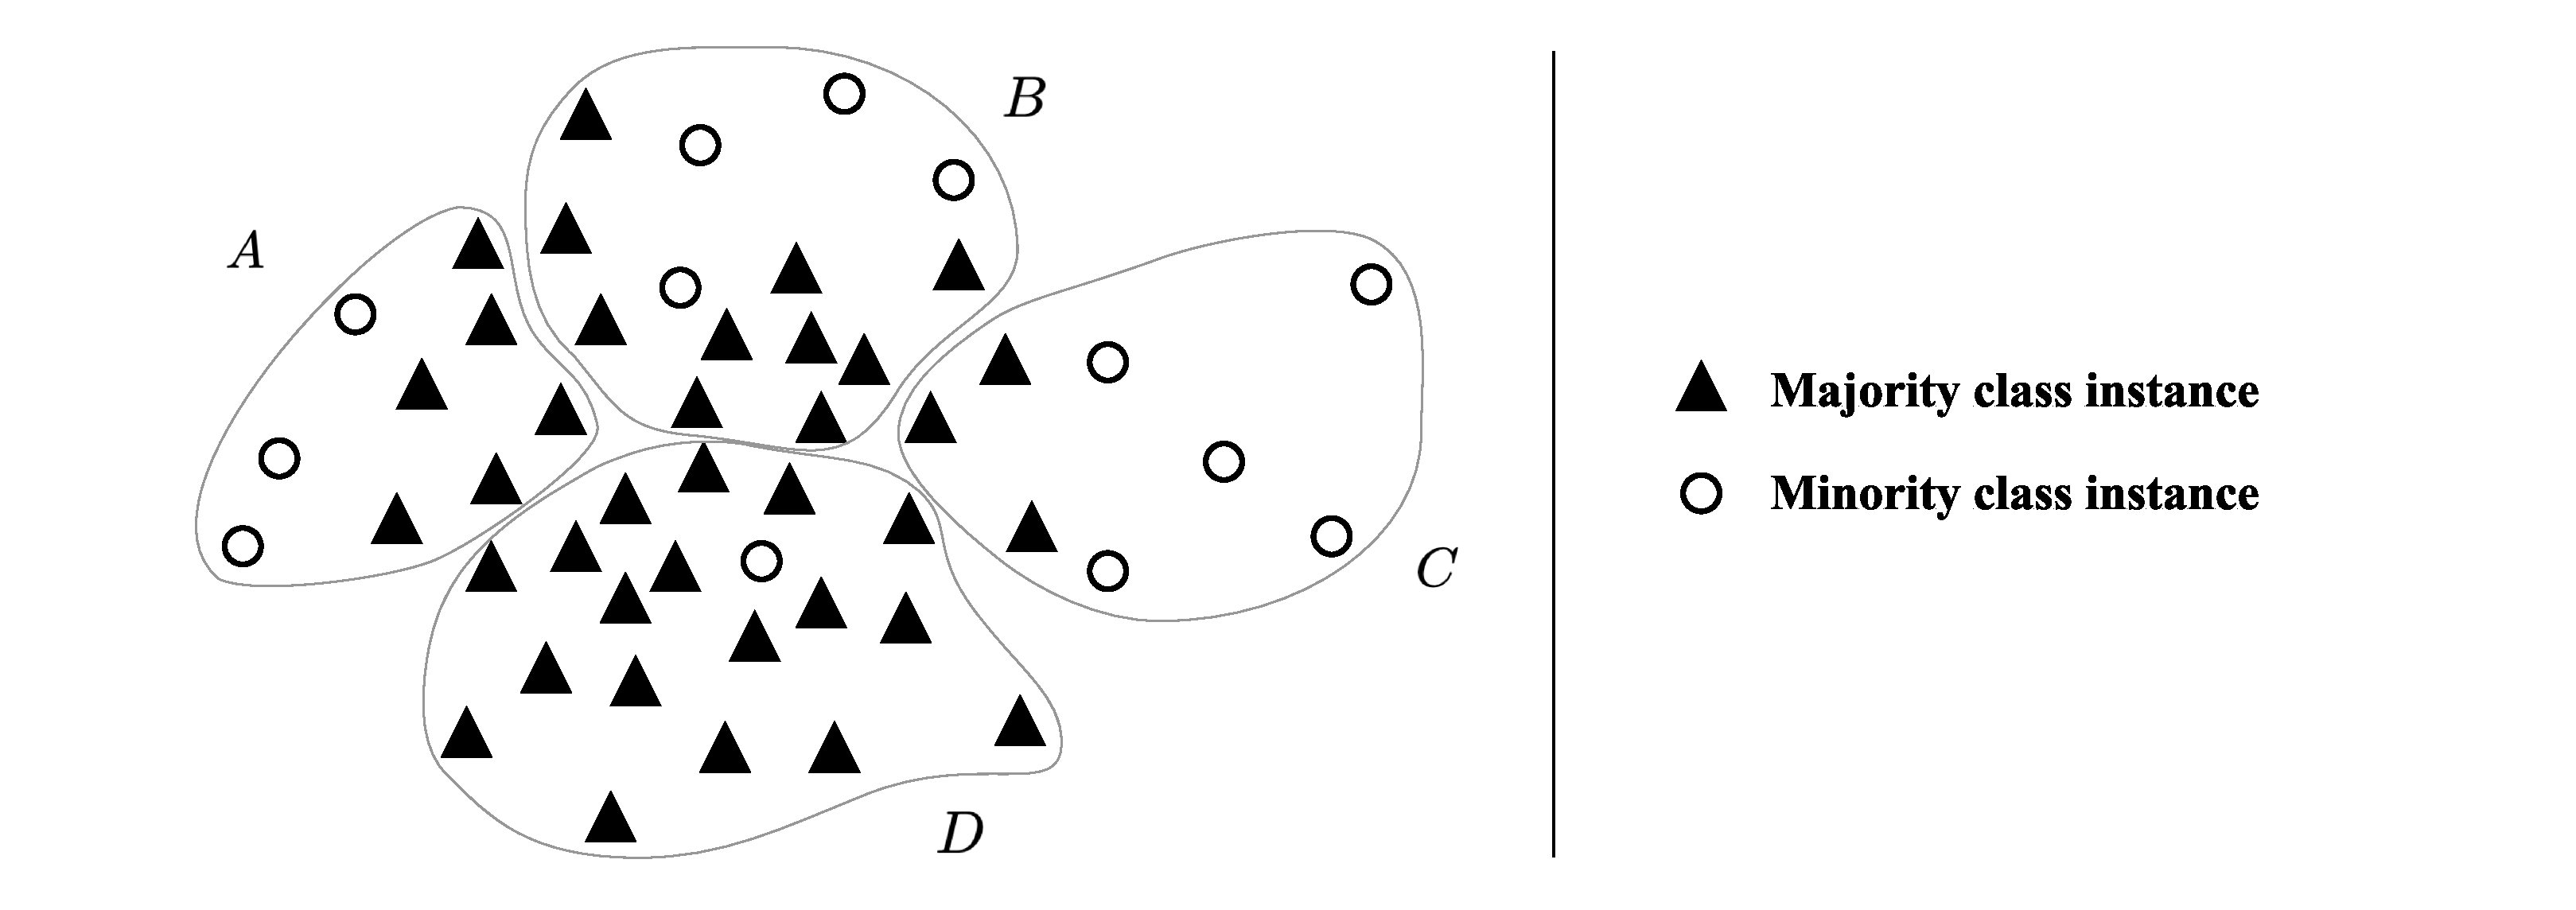
\includegraphics[width=1\linewidth]{complex_input_space_example}
    \caption[Example of a complex input space.]{%
        Example of a complex input space. In this example, a classifier
        would need to separate the minority class' samples across 4
        distinguishable clusters (A, B, C and D).
    }~\label{fig:complex_input_space_example}
\end{figure}

The efficacy of K-means SMOTE is tested using different types of classifiers.
To do so, we employ both commonly used and/or state-of-the-art oversamplers as
benchmarking methods: Random oversampling (ROS), SMOTE and Borderline-SMOTE
(B-SMOTE) \cite{Han2005}. Also as a baseline score we include classification
results without the use of any resampling method.

This paper is organized in 5 sections: section \ref{sec:sota-kmeans} provides an
overview of the state-of-art, section \ref{sec:methodology-kmeans} describes the
proposed methodology, section \ref{sec:results-kmeans} covers the results and
discussion and section \ref{sec:conclusion-kmeans} presents the conclusions taken from
this study.

This paper's main contributions are:
\begin{itemize}
    \item Propose a cluster-based multiclass oversampling method appropriate
        for LULC classification and compare its performance with the remaining
        oversamplers in a multiclass context with seven benchmark LULC
        classification datasets. Allows us to check the oversamplers'
        performance across benchmark LULC datasets.
    \item Introducing a cluster-based oversampling algorithm within the remote
        sensing domain, as well as comparing its performance with the remaining
        oversamplers in a multiclass context.
    \item Make available to the remote sensing community the implementation
        of the algorithm in a Python library and the experiment's source
        code.
\end{itemize}

\section{Imbalanced Learning Approaches}~\label{sec:sota-kmeans}

Imbalanced learning has been addressed in three different ways:
over/undersampling, cost-sensitive training and changes/adaptations in the
learning algorithms \cite{Kaur2019}. These approaches impact different
phases of the learning process, while over/undersampling can be seen as a
pre-processing step, cost-sensitive and changes in the algorithm imply a more
customized and complex intervention in the algorithms. In this
section, we focus on previous work related with resampling methods, while
providing a brief explanation of cost-sensitive and algorithmic level solutions.

All of the most common classifiers used for LULC classification tasks
\cite{Khatami2016, Gavade2019} are sensitive to class imbalance
\cite{Blagus2010}. Algorithm-based approaches typically focus on adaptations
based on ensemble classification methods \cite{Mellor2015} or common
non-ensemble based classifiers such as Support Vector Machines \cite{Shao2014}.
In \cite{Lee2016}, the reported results show that algorithm-based methods have
comparable performance to resampling methods.

Cost-sensitive solutions refer to changes in the importance attributed to each
instance through a cost matrix \cite{Huang2016,Cui2019,Dong2017}. A
relevant cost sensitive solution
\cite{Huang2016} uses  the inverse class frequency (i.e., $1/|C_i|$, where $C_i$ refers
to the frequency of class $i$) to give higher weight to
minority classes. Cui et al. \cite{Cui2019} extended this method by adding a
hyperparameter $\beta$ to class weights as $(1-\beta)/(1-\beta^{|C_i|})$. When
$\beta=0$, no re-weighting is done. When $\beta\rightarrow 1$, weights are the
inverse of the frequency class matrix. Another method \cite{Dong2017} explores
adaptations of Cross-entropy classification loss by adding different
formulations of class rectification loss.

Resampling (over/undersampling) is the most common approach to imbalanced
learning in machine
learning in general and remote sensing in particular \cite{Feng2019}. The
generation of artificial instances (i.e., augmenting the dataset), based on
rare instances, is done independently of any other step in the learning
process. Once the procedure is applied, any standard machine learning
algorithm can be used. Its simplicity makes resampling strategies particularly
appealing for any user (especially the non-sophisticated user) interested in
applying several classifiers, while maintaining a simple approach. It is also
important to notice that over/undersampling methods can also be easily applied
to multiclass problems, common in LULC classification tasks.

\subsection{Non-informed resampling methods}

There are two main non-informed resampling methods. Random Oversampling (ROS)
generates artificial instances through random duplication of minority class
instances. This method is used in remote sensing for its simplicity
\cite{Sharififar2019, Hounkpatin2018}, even though its mechanism makes the
classifier prone to overfitting \cite{Krawczyk2016}. \cite{Hounkpatin2018}
found that using ROS returned worse results than keeping the original
imbalance in their dataset.

A few of the recent remote sensing studies employed Random Undersampling (RUS)
\cite{Ferreira2019}, which randomly removes instances belonging to majority
classes. Although it's not as prone to overfitting as ROS, it incurs into
information loss by eliminating instances from the majority class
\cite{Feng2019}, which can be detrimental to the quality of the results.

Another disadvantage of non-informed resampling methods is their
performance-wise inconsistency across classifiers. ROS' impact on the Indian
Pines dataset was found inconsistent between Random Forest Classifiers (RFC)
and Support Vector Machines (SVM) and lowered the predictive power of an
artificial neural network (ANN) \cite{Maxwell2018}. Similarly, RUS is found to
generally lead to a lower overall accuracy due to the associated information
loss \cite{Maxwell2018}.

\subsection{Heuristic methods}

The methods presented in this section appear as a means to overcome the
insufficiencies found in non-informed resampling. They use either local or
global information to generate new, relevant, non-duplicated instances to
populate the minority classes and/or remove irrelevant instances from majority
classes. In a comparative analysis between over- and undersamplers' performance
for LULC classification \cite{Feng2018} using the rotation forest ensemble
classifier, authors found that oversampling methods consistently outperform
undersampling methods. This result led us to exclude undersampling from our
study.

SMOTE \cite{Chawla2002} was the first heuristic oversampling algorithm to be
proposed and has been the most popular one since then, likely due to its fair
degree of simplicity and quality of generated data. It takes a random minority
class sample and introduces synthetic instances along the line segment that
join a random $k$ minority class nearest neighbor to the selected sample.
Specifically, a single synthetic sample $\overrightarrow{z}$ is generated
within the line segment of a randomly selected minority class
instance $\overrightarrow{x}$ and one of its $k$ nearest
neighbors $\overrightarrow{y}$ such that $\overrightarrow{z} =
\alpha\overrightarrow{x}+(1-\alpha)\overrightarrow{y}$, where $\alpha$ is a
random real number between 0 and 1, as shown in
Figure \ref{fig:smote_example}.

\begin{figure}
	\centering
	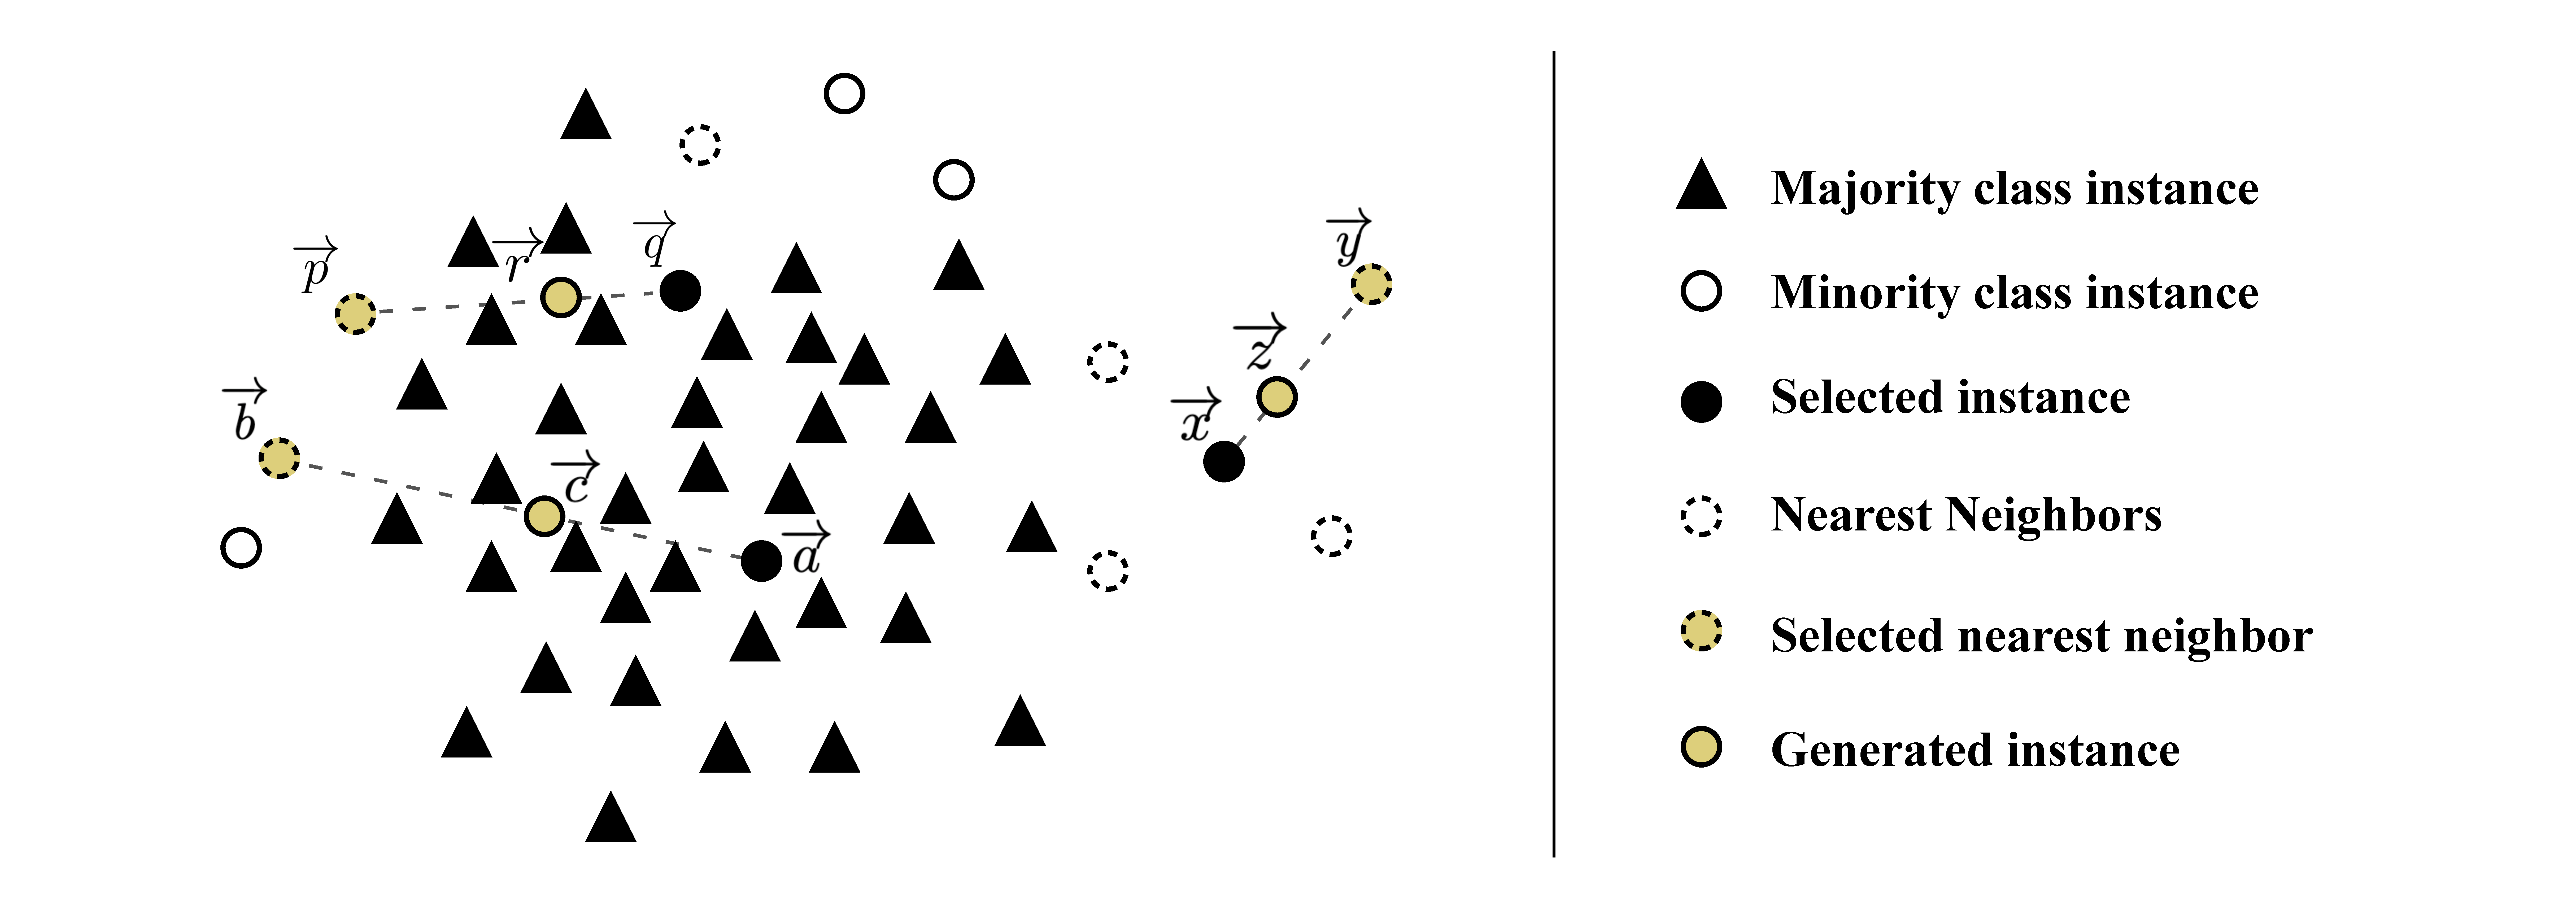
\includegraphics[width=1\linewidth]{smote_example}
    \caption[Example of SMOTE's data generation process]{Example of SMOTE's
        data generation process. SMOTE randomly selects instance
        $\protect\overrightarrow{x}$ and randomly selects one of its k-nearest
        neighbors $\protect\overrightarrow{y}$ to produce
        $\protect\overrightarrow{z}$.  Noisy instance
        $\protect\overrightarrow{r}$ was generated by randomly selecting
        $\protect\overrightarrow{q}$ and randomly selecting its nearest
        neighbor $\protect\overrightarrow{p}$ from a different minority class
        cluster. Noisy instance $\protect\overrightarrow{c}$ was generated by
        randomly selecting the noisy minority class instance
        $\protect\overrightarrow{a}$ and one of its nearest neighbors
        $\protect\overrightarrow{b}$.
    }~\label{fig:smote_example}
\end{figure}

A number of studies implement SMOTE within the LULC classification context and
reported improvements on the quality of the trained predictors
\cite{Jozdani2019, Bogner2018}. Another study proposes an adaptation of SMOTE
on an algorithmic level for deep learning applications \cite{Zhu2020}. This
method combines both typical computer vision data augmentation techniques,
such as image rotation, scaling and flipping on the generated instances to
populate minority classes. Another algorithmic implementation is the
variational semi-supervised learning model \cite{Cenggoro2018}. It consists of
a generative model that allows learning from both labeled and unlabeled
instances while using SMOTE to balance the data.

Despite SMOTE's popularity, its limitations have motivated the development of
more sophisticated oversampling algorithms \cite{Douzas2019, Han2005, Ma2017,
Douzas2017, Douzas2018, HaiboHe2008}. \cite{Douzas2019} identify four major
weaknesses of the SMOTE algorithm, which can be summarized as:

\begin{enumerate}
    \item Generation of noisy instances due to random selection of a
        minority instance to oversample. The random
        selection of a minority instance makes SMOTE
        oversampling prone to the amplification of existing noisy data. This
        has been addressed by variants such as B-SMOTE \cite{Han2005} and
        ADASYN \cite{HaiboHe2008}. 

    \item Generation of noisy instances due to the selection of the $k$
        nearest neighbors. In the event an instance
        (or a small number thereof) is not noisy but is isolated from the
        remaining clusters, known as the "small disjuncts problem"
        \cite{holte1989}, much like sample $\overrightarrow{b}$ from Figure
        \ref{fig:smote_example}, the selection of any nearest neighbor of the
        same class will have a high likelihood of producing a noisy sample.

    \item Generation of nearly duplicated instances. Whenever the linear
        interpolation is done between two instances that are close to each
        other, the generated instance becomes very similar to its parents and
        increases the risk of overfitting. G-SMOTE \cite{Douzas2019} attempts
        to address both the $k$ nearest neighbor selection mechanism problem
        as well as the generation of nearly duplicated instances problem. 

    \item Generation of noisy instances due to the use of
        instances from two different minority class clusters.
        Although an increased $k$ could potentially avoid the previous
        problem, it can also lead to the generation of artificial data between
        different minority clusters, as depicted Figure
        \ref{fig:smote_example} with the generation of point
        $\overrightarrow{r}$ using minority class instances $\overrightarrow{p}$ and $\overrightarrow{q}$.
        Cluster-based oversampling methods attempt to address this problem. 
\end{enumerate}

This last issue, the generation of noisy instances due to the existence of
several minority class clusters, is particularly relevant in remote sensing.
It is frequent that instances belonging to the same minority class can have
different spectral signatures, meaning that they will be clustered in
different parts of the input space. For example, in the classification of a
hyperspectral scene dominated by agricultural activities, patches relating to
urban areas may constitute a minority class. These patches frequently refer to
different types of land use, such as housing regions, small gardens, asphalt
roads, etc., all these containing different spectral signatures. In this
context, the use of SMOTE will lead to the generation of noisy instances of
the minority class. This problem can be efficiently mitigated through the use
of a cluster-based oversampling method. According to our literature review
cluster-based oversampling approaches have never been applied in the context
of remote sensing. On the other hand, while there are references of the
application of cluster-based oversampling in the context of machine
learning~\cite{Santos2015, Douzas2017, Ma2017, Douzas2018}, the multiclass
case is rarely addressed, which is a fundamental requirement for the
application of oversampling in the context of LULC. 

Cluster-based oversampling approaches introduce an additional layer to SMOTE's
selection mechanism, which is done through the inclusion of a clustering
process. This ensures that both between-class data balance and
within-class balance is preserved. The
self-organizing map oversampling (SOMO) \cite{Douzas2017} algorithm transforms
the dataset into a 2-dimensional input, where the areas with the highest
density of minority samples are identified. SMOTE is then used to oversample
each of the identified areas separately. ClUstered REsampling SMOTE
(CURE-SMOTE) \cite{Ma2017} applies a hierarchical clustering
algorithm to discard isolated minority instances before applying SMOTE.
Although it avoids noise generation problems, it ignores within-class data
distribution. Another method \cite{Santos2015} uses K-means to cluster the
entire input space and applies SMOTE to clusters with the fewest
instances, regardless of their class label. The label of the
generated instance is copied from one of its parents.
This method cannot ensure a balanced dataset since class imbalance is not
specifically addressed, but rather dataset imbalance.

\begin{figure}
	\centering
	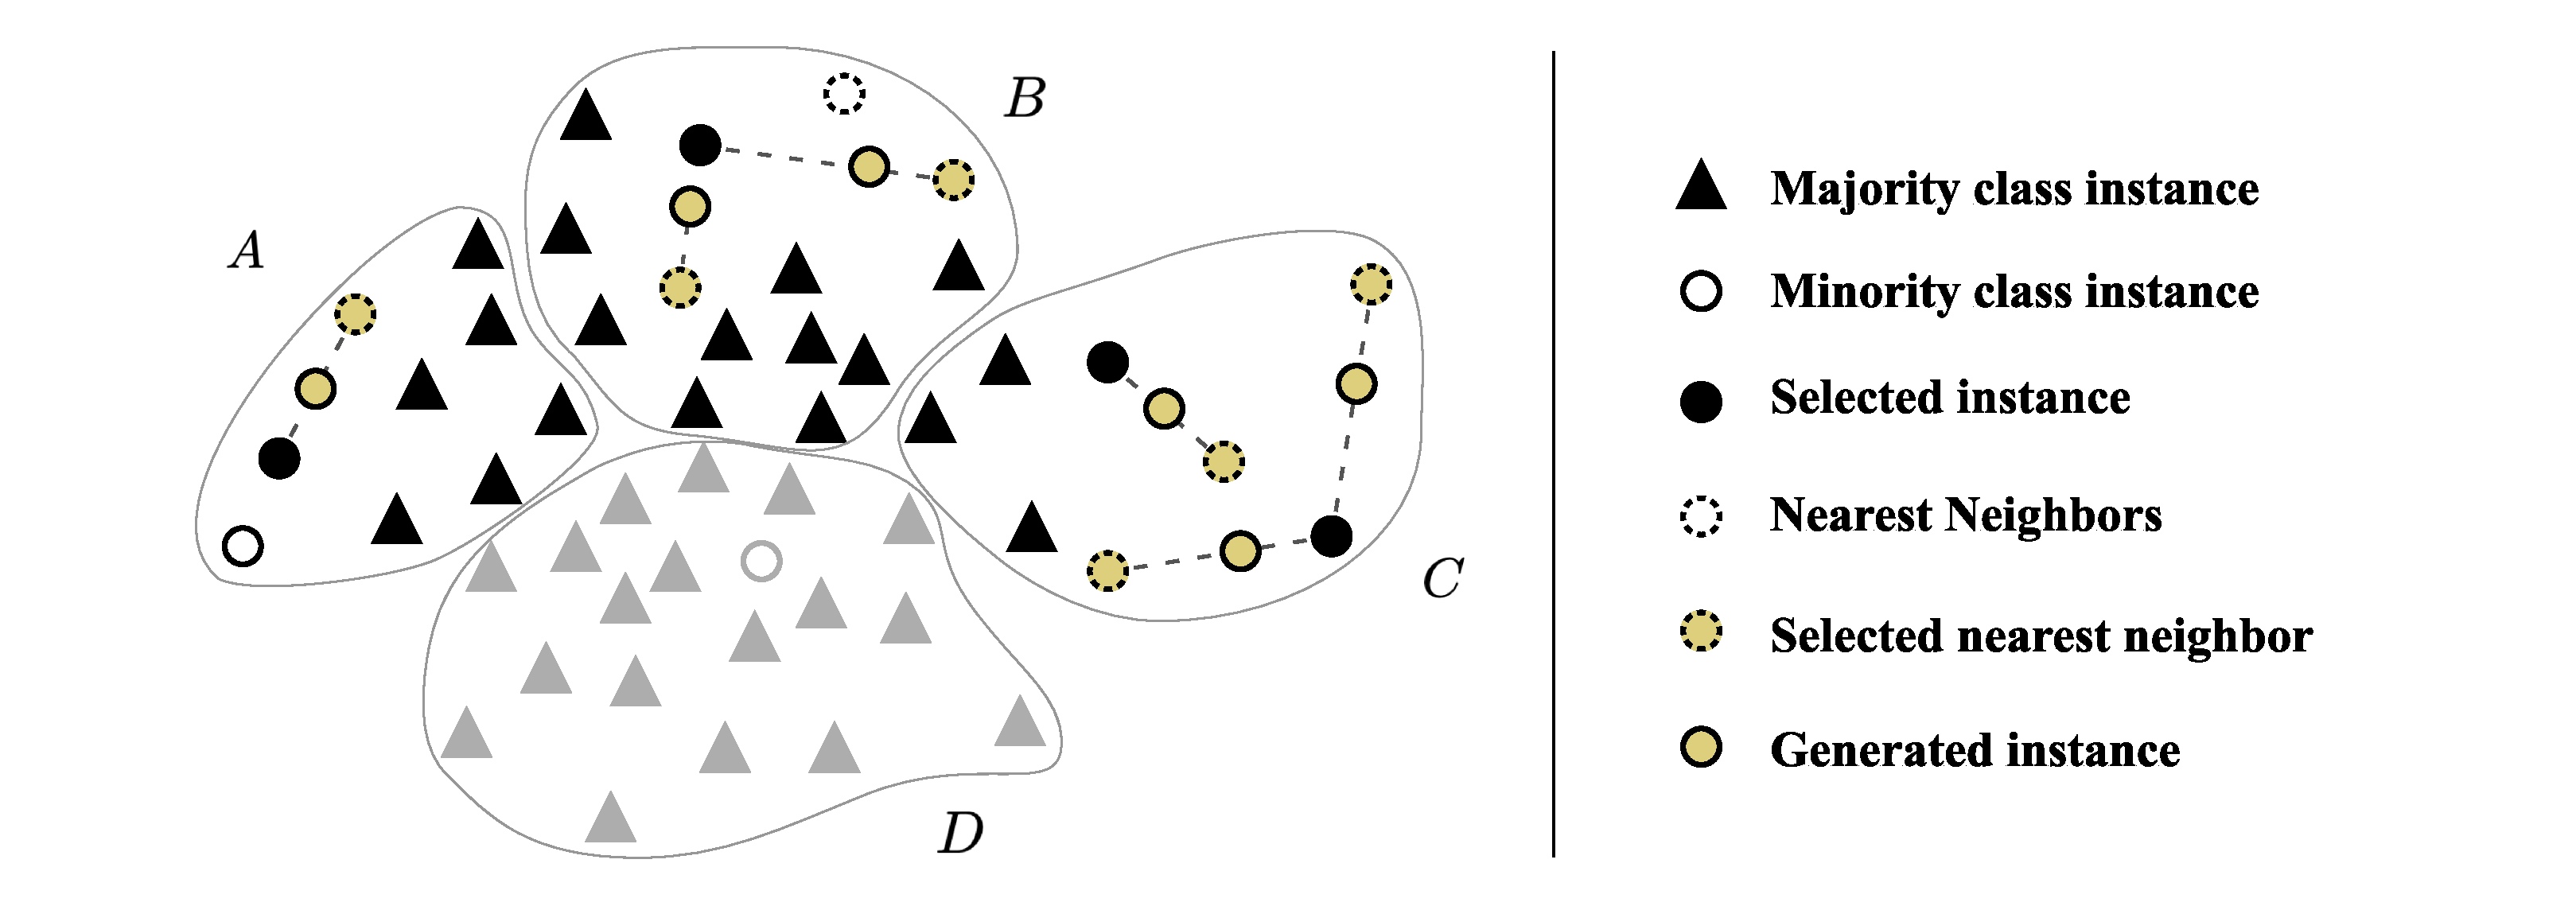
\includegraphics[width=1\linewidth]{kmeans_smote_example}
    \caption[Example of K-means SMOTE's data generation process.]{Example of
        K-means SMOTE's data generation process. Clusters $A$, $B$ and $C$ are
        selected for oversampling, whereas cluster $D$ was rejected due to its
        high imbalance ratio. The oversampling is done using the SMOTE
        algorithm and the $k$ nearest neighbors selection only considers
        instances within the same cluster.
    }~\label{fig:kmeans_smote_example}
\end{figure}

K-means SMOTE~\cite{Douzas2018} avoids noisy data generation by modifying the
data selection mechanism. It employs $k$-means clustering to identify safe
areas using cluster-specific Imbalance Ratio (IR, defined by
$\frac{count(C_{majority})}{count(C_{minority})}$) and determine the quantity
of generated samples per cluster based on a density measure. These samples are
finally generated using the SMOTE algorithm. The K-means SMOTE's data
generation process is depicted in Figure~\ref{fig:kmeans_smote_example}. Note
that the number of samples generated for each cluster varies according to the
sparsity of each cluster (the sparser the cluster is, the more samples will be
generated) and a cluster is rejected if the cluster's IR surpasses the
threshold.  Therefore, this method can be combined with any data generation
mechanism, such as G-SMOTE.  Also K-means SMOTE includes the SMOTE algorithm
as a special case when the number of clusters is set to one. Consequently,
K-means SMOTE returns results as good as or better than SMOTE.

Although no other study was found to implement cluster-based oversampling,
another study \cite{Douzas2019rs} compared the performance of SMOTE, ROS,
ADASYN, B-SMOTE and G-SMOTE in a highly imbalanced LULC classification dataset.
The authors found that G-SMOTE consistently outperformed the remaining
oversampling algorithms regardless of the classifier used.

\section{Methodology}\label{sec:methodology-kmeans}

The purpose of this work is to understand the performance of K-means SMOTE as
opposed to other popular and/or state-of-the-art oversamplers for LULC
classification. This is done using 7 datasets with predominantly land use
information, along with 3 evaluation metrics and 3 classifiers to evaluate the
performance of oversamplers. In this section we describe the datasets,
evaluation metrics, oversamplers, classifiers and software used as well as the
procedure developed.

\subsection{Datasets}

The datasets used were extracted from publicly available hyperspectral scenes.
Information regarding each of these scenes is provided in this subsection.
The data collection and preprocessing pipeline is shown in
Figure~\ref{fig:data_preprocessing_pipeline} and is common to all
hyperspectral scenes:

\begin{enumerate}
    
    \item Data collection of publicly available hyperspectral scenes.
        The original hyperspectral scenes and ground truth data were collected
        from a single publicly available data repository available
        \href{http://www.ehu.eus/ccwintco/index.php?title=Hyperspectral_Remote_Sensing_Scenes}{here}.

    \item Conversion of each hyperspectral scene to a structured
        dataset and removal of instances with no associated LULC class. This
        done to reshape the dataset from $(h,w,b+gt)$  into a conventional
        dataframe of shape $(h*w,b+gt)$, where $gt$, $h$, $w$ and $b$
        represents the ground truth, height, width and number of bands in the
        scene, respectively. The pixels without ground truth information are
        discarded from further analysis.

    \item Stratified random sampling to maintain similar class
        proportions on a sample of 10\% of each dataset. This is done by
        computing the relative class frequencies in the original hyperspectral
        scene (minus the class representing no ground truth availability) and
        retrieving a sample that ensures the original relative class
        frequencies remain unchanged.

    \item Removal of instances belonging to a class with frequency
        lower than 20 or higher than 1000. This is done to maintain the
        datasets to a practicable size due to computational constraints, while
        conserving the relative LULC class frequencies and data distribution. 

    \item Data normalization using the MinMax scaler. This ensures all
        features (i.e., bands) are in the same scale. In this case, the data
        was rescaled between 0 and 1.

\end{enumerate}

Table~\ref{tab:datasets_description_kmeans} provides a description of the final
datasets used for this work, sorted according to its IR.
Figure~\ref{fig:scenes_lulc} shows the original hyperspectral scene out of which
the dataset used in this experiment were extracted. In the representation of
the ground truth of these scenes, the blue regions in the ground truth of each
hyperspectral scene represent unlabeled regions (i.e., no  ground truth is
available). Particularly, in the Botswana and Kennedy Space Center scenes the
truth was photointerpreted in more limited regions of the scene. However, the
scenes are still represented as they are in order to maintain a standardized
analysis over all datasets extracted for the experiment.

\begin{figure}
	\centering
	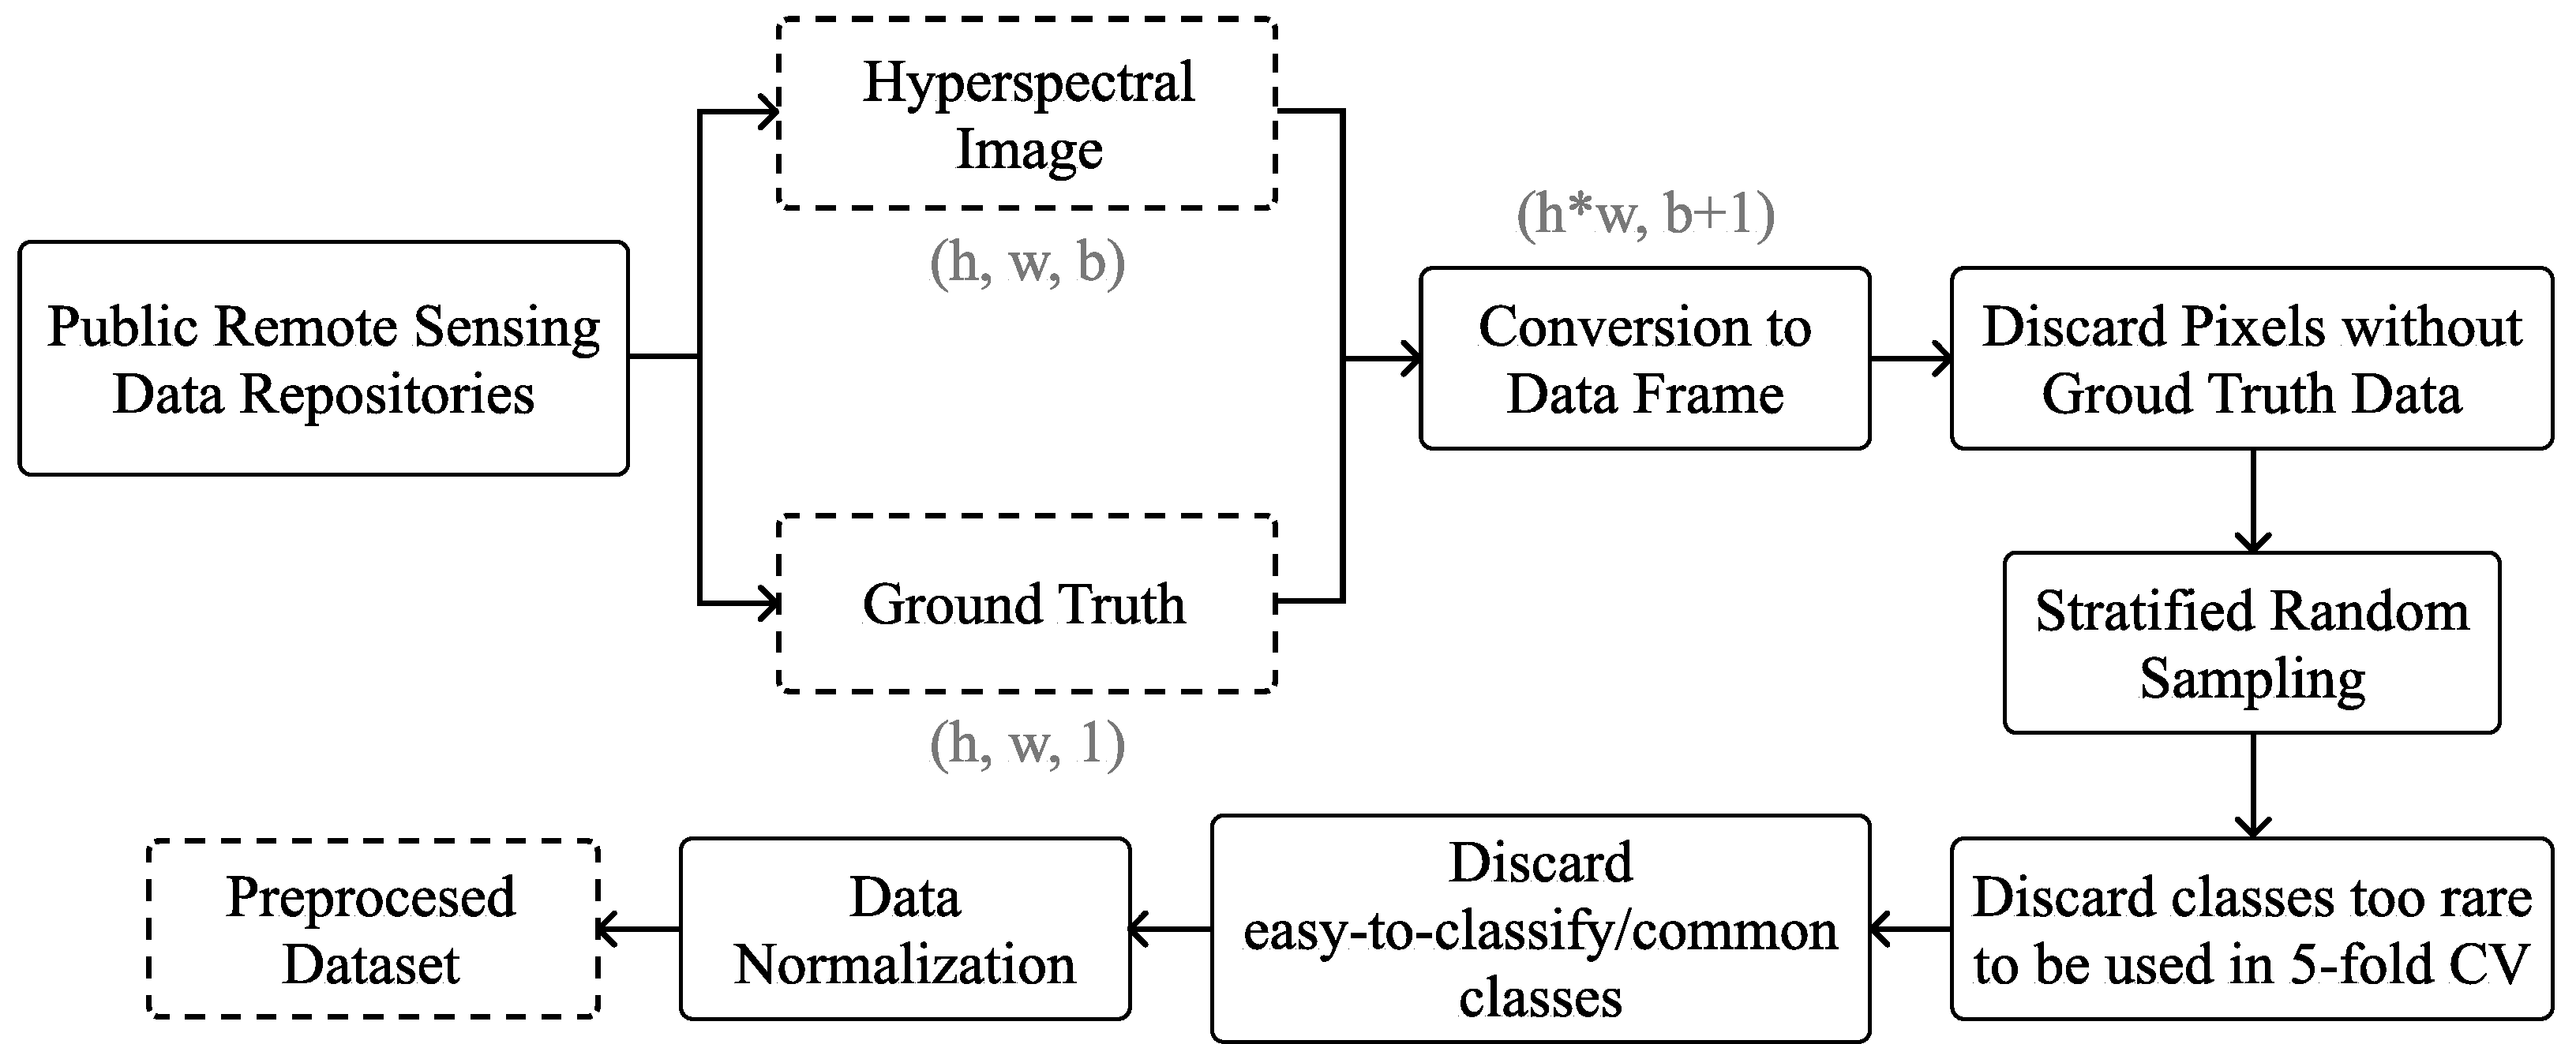
\includegraphics[width=.75\linewidth]{data_preprocessing_pipeline}
    \caption{Data collection and preprocessing
    pipeline.}~\label{fig:data_preprocessing_pipeline}
\end{figure}

\begin{table}
	\centering
    \addtolength{\leftskip} {-2cm}
    \addtolength{\rightskip}{-2cm}
    \pgfplotstabletypeset[
        col sep=comma,
        string type,
        every head row/.style={%
            before row=\toprule,
            after row=\midrule
        },
        every last row/.style={after row=\bottomrule},
        string type,
    ]{figures/kmeans-smote-lulc/datasets_description.csv}
    \caption{Description of the datasets used for this
    experiment.}~\label{tab:datasets_description_kmeans}
\end{table}

\subsubsection*{Botswana}

The Botswana scene was acquired by the Hyperion sensor on the NASA EO-1
satellite over the Okavango Delta, Botswana in 2001-2004 at a 30m spatial
resolution. Data preprocessing was performed by the UT Center for Space
Research. The scene comprises a $1476 \times 256$ pixels with 145 bands and 14
classes regarding land cover types in seasonal and occasional swamps, as well
as drier woodlands (see Figure~\ref{fig:botswana}). The classes with
rare instances are Short mopane and Hippo grass.

\subsubsection*{Pavia Center and University}

Both Pavia Center and University scenes were acquired by the ROSIS sensor.
These scenes are located in Pavia, northern Italy. Pavia Center is a $1096
\times 1096$ pixels image with 102 spectral bands, whereas Pavia University is
a $610 \times 610$ pixels image with 103 spectral bands. Both images have a
geometrical resolution of 1.3m and their ground truths are
composed of 9 classes each (see Figures~\ref{fig:pavia_center}
and~\ref{fig:pavia_university}). After data preprocessing, the classes
with rare instances are Asphalt and Bitumen (the class Shadows was removed for
being too rare for cross validation after random sampling).

\subsubsection*{Kennedy Space Center}

The Kennedy Space Center scene was acquired by the AVIRIS sensor over the
Kennedy Space Center, Florida, on March 23, 1996. Out of the original 224
bands, water absorption and low SNR bands were removed and a total of 176
bands at a spatial resolution of 18m are used. The scene is a $512 \times 614$
pixel image and contains a total of 16 classes (see
figure~\ref{fig:kennedy_space_center}). The classes with rare instances
are hardwood swamp, slash pine and willow swamp (both hardwood swamp and slash
pine were removed for being too rare for cross validation after random
sampling).

\subsubsection*{Salinas and Salinas-A}

These scenes were collected by the AVIRIS sensor over Salinas Valley,
California and contain at-sensor radiance data. Salinas is a $512 \times 217$
pixels image with 224 bands and 16 classes regarding vegetables, bare soil and
vineyard fields (see Figure~\ref{fig:salinas}). Salinas-A, a subscene of
Salinas, comprises $86 \times 83$ pixels and contains 6 classes regarding
vegetables (see Figure~\ref{fig:salinas_a}). These scenes have a geometrical
resolution of 3.7m. Salinas-A's minority class has the label
``Brocoli\_green\_weeds\_1'' and Salina's minority class has the label
``Lettuce\_romaine\_6wk''

\subsubsection*{Indian Pines} 

The Indian Pines scene~\cite{Baumgardner2015} was collected on June 12, 1992
and consists of AVIRIS hyperspectral image data covering the Indian Pine Test
Site 3, located in North-western Indiana, USA. As a subset of a larger scene,
it is composed of $145 \times 145$ pixels (see Figure~\ref{fig:indian_pines})
and 220 spectral reflectance bands in the wavelength range 400 to 2500
nanometers at a spatial resolution of 20m. Approximately two thirds of
this scene is composed by agriculture and the other third is composed of
forest and other natural perennial vegetation. Additionally, the scene also
contains low density buildup areas. The classes with rare instances are
Alfalfa, Oats, Grass-pasture-mowed, Wheat and Stone-Steel-Towers (which
removed for being too rare for cross validation after random sampling).  After
data preprocessing, the classes with rare instances are Corn,
Buildings-Grass-Trees-Drives and Grass-Pasture.

\begin{figure}
	\centering
	\begin{subfigure}{.24\textwidth}
		\centering
		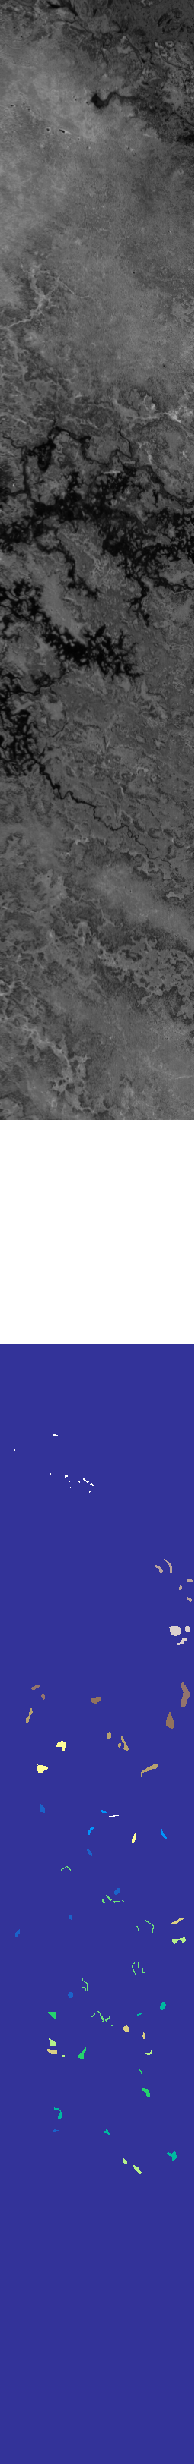
\includegraphics[height=1.5\linewidth]{botswana}
		\subcaption{{\medbreak}}\label{fig:botswana}
	\end{subfigure}
	\begin{subfigure}{.24\textwidth}
		\centering
		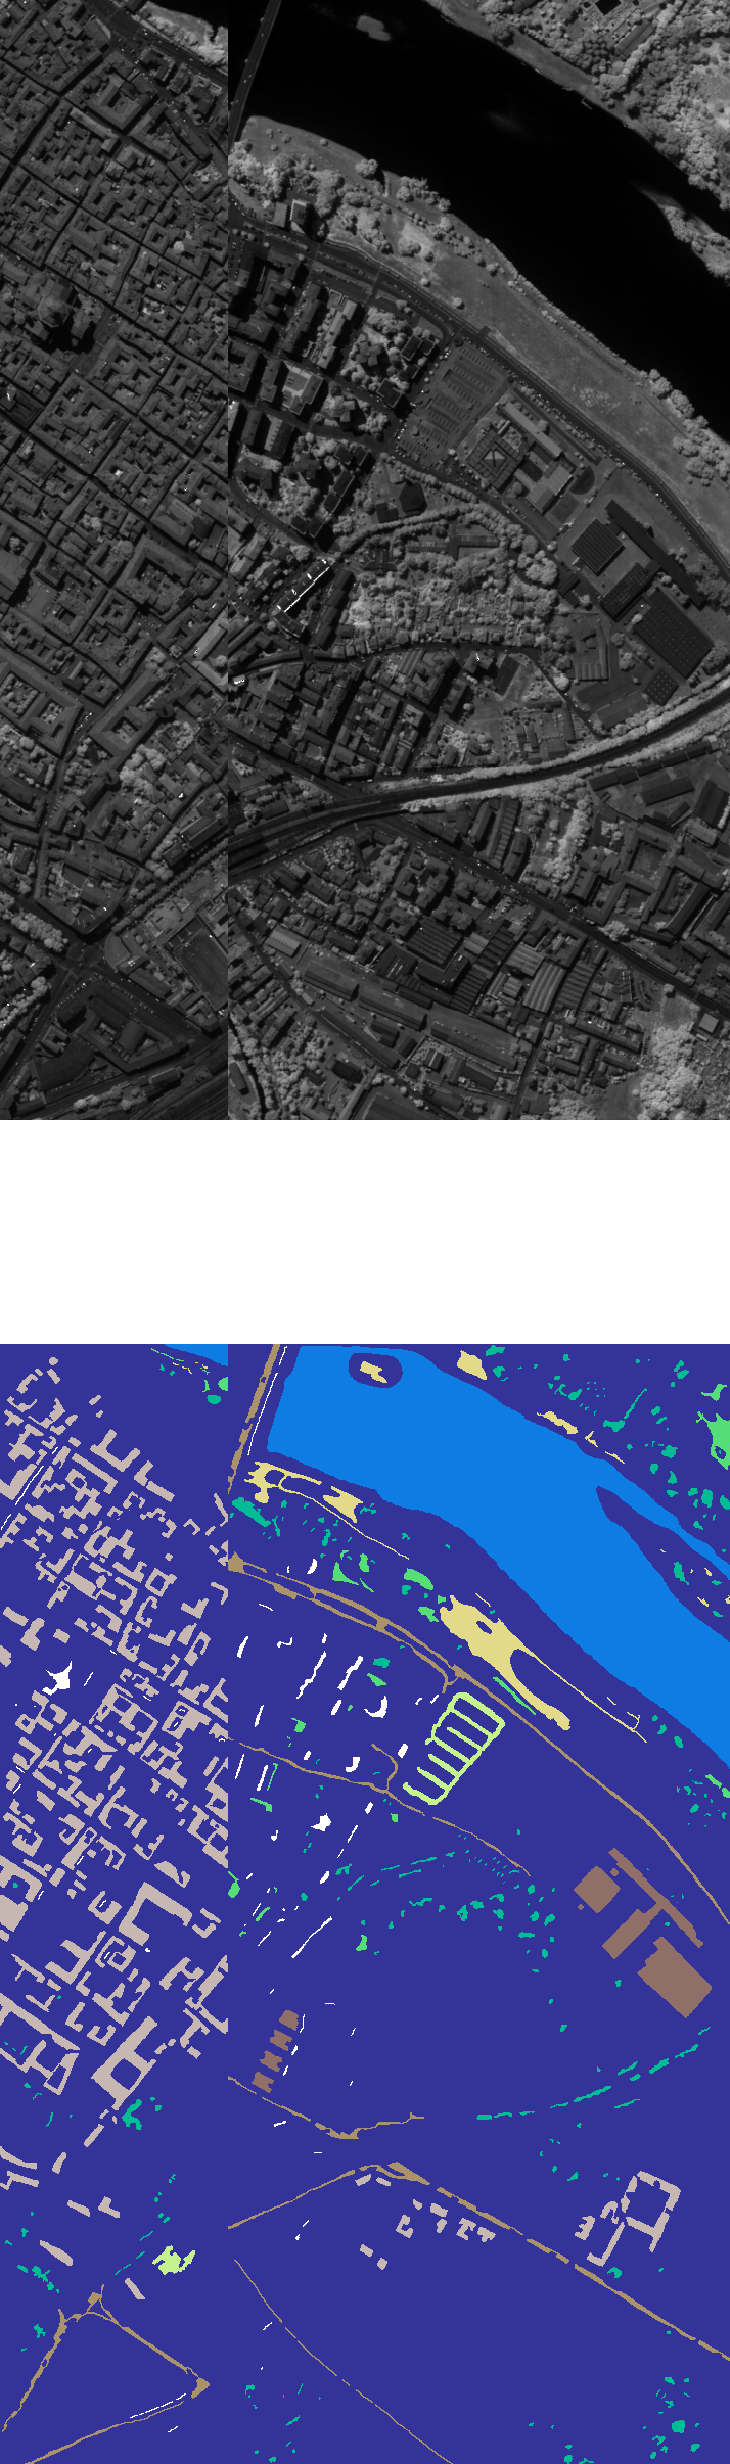
\includegraphics[height=1.5\linewidth]{pavia_centre}
		\subcaption{{\medbreak}}\label{fig:pavia_center}
	\end{subfigure}
	\begin{subfigure}{.24\textwidth}
		\centering
		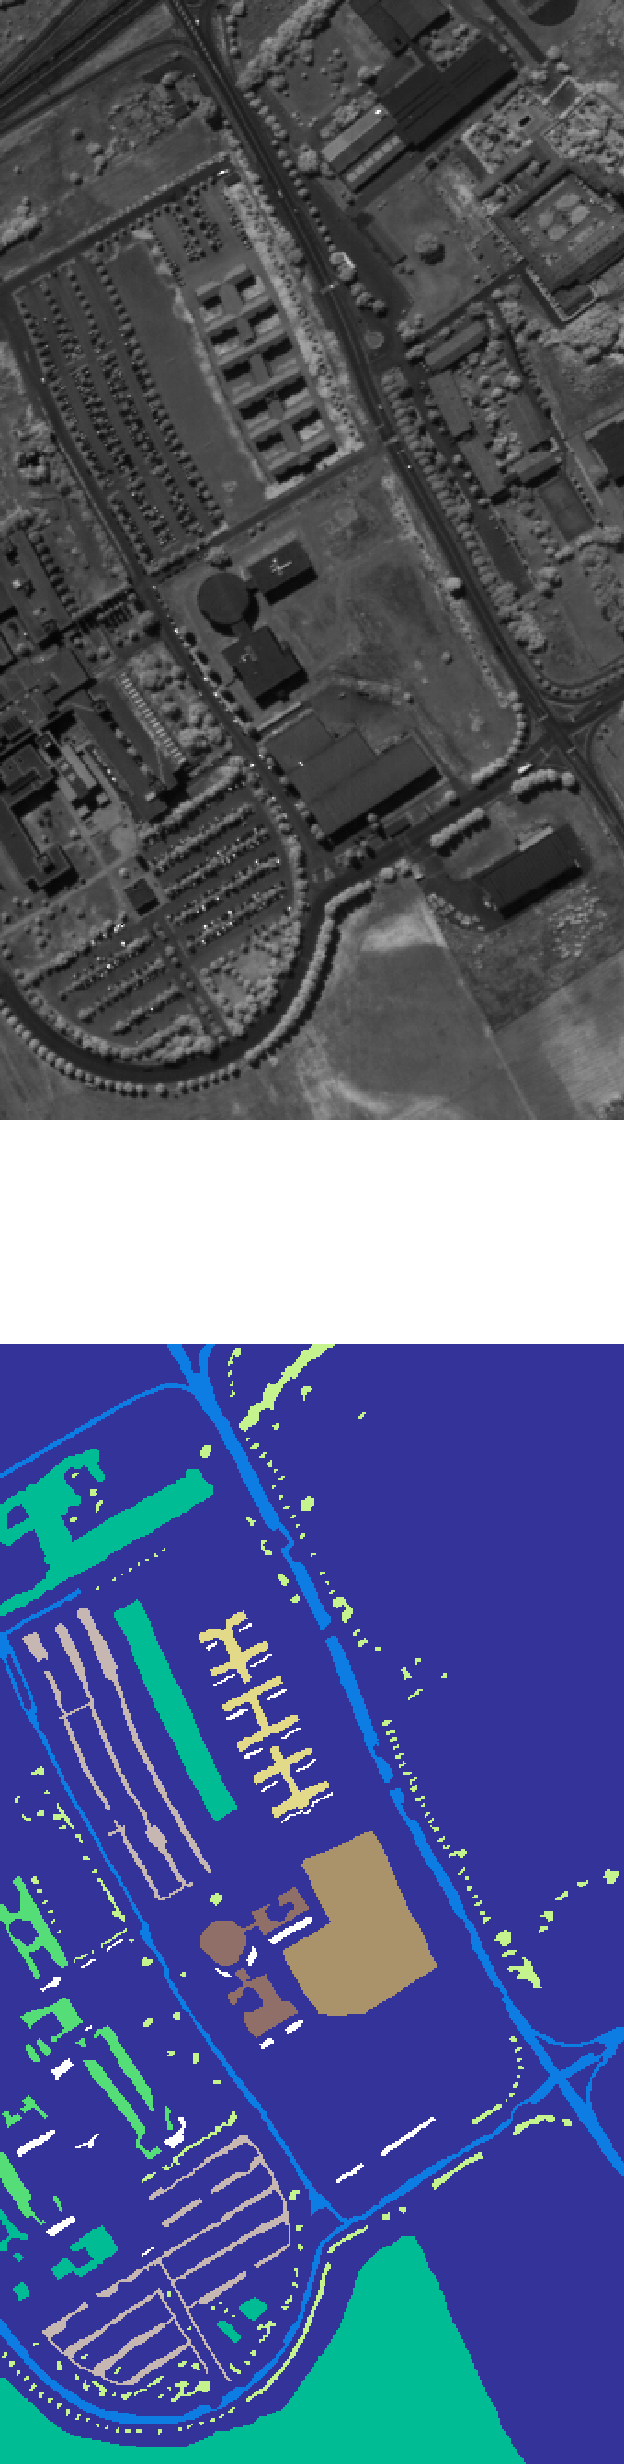
\includegraphics[height=1.5\linewidth]{pavia_university}
		\subcaption{{\medbreak}}\label{fig:pavia_university}
	\end{subfigure}
	\begin{subfigure}{.24\textwidth}
		\centering
		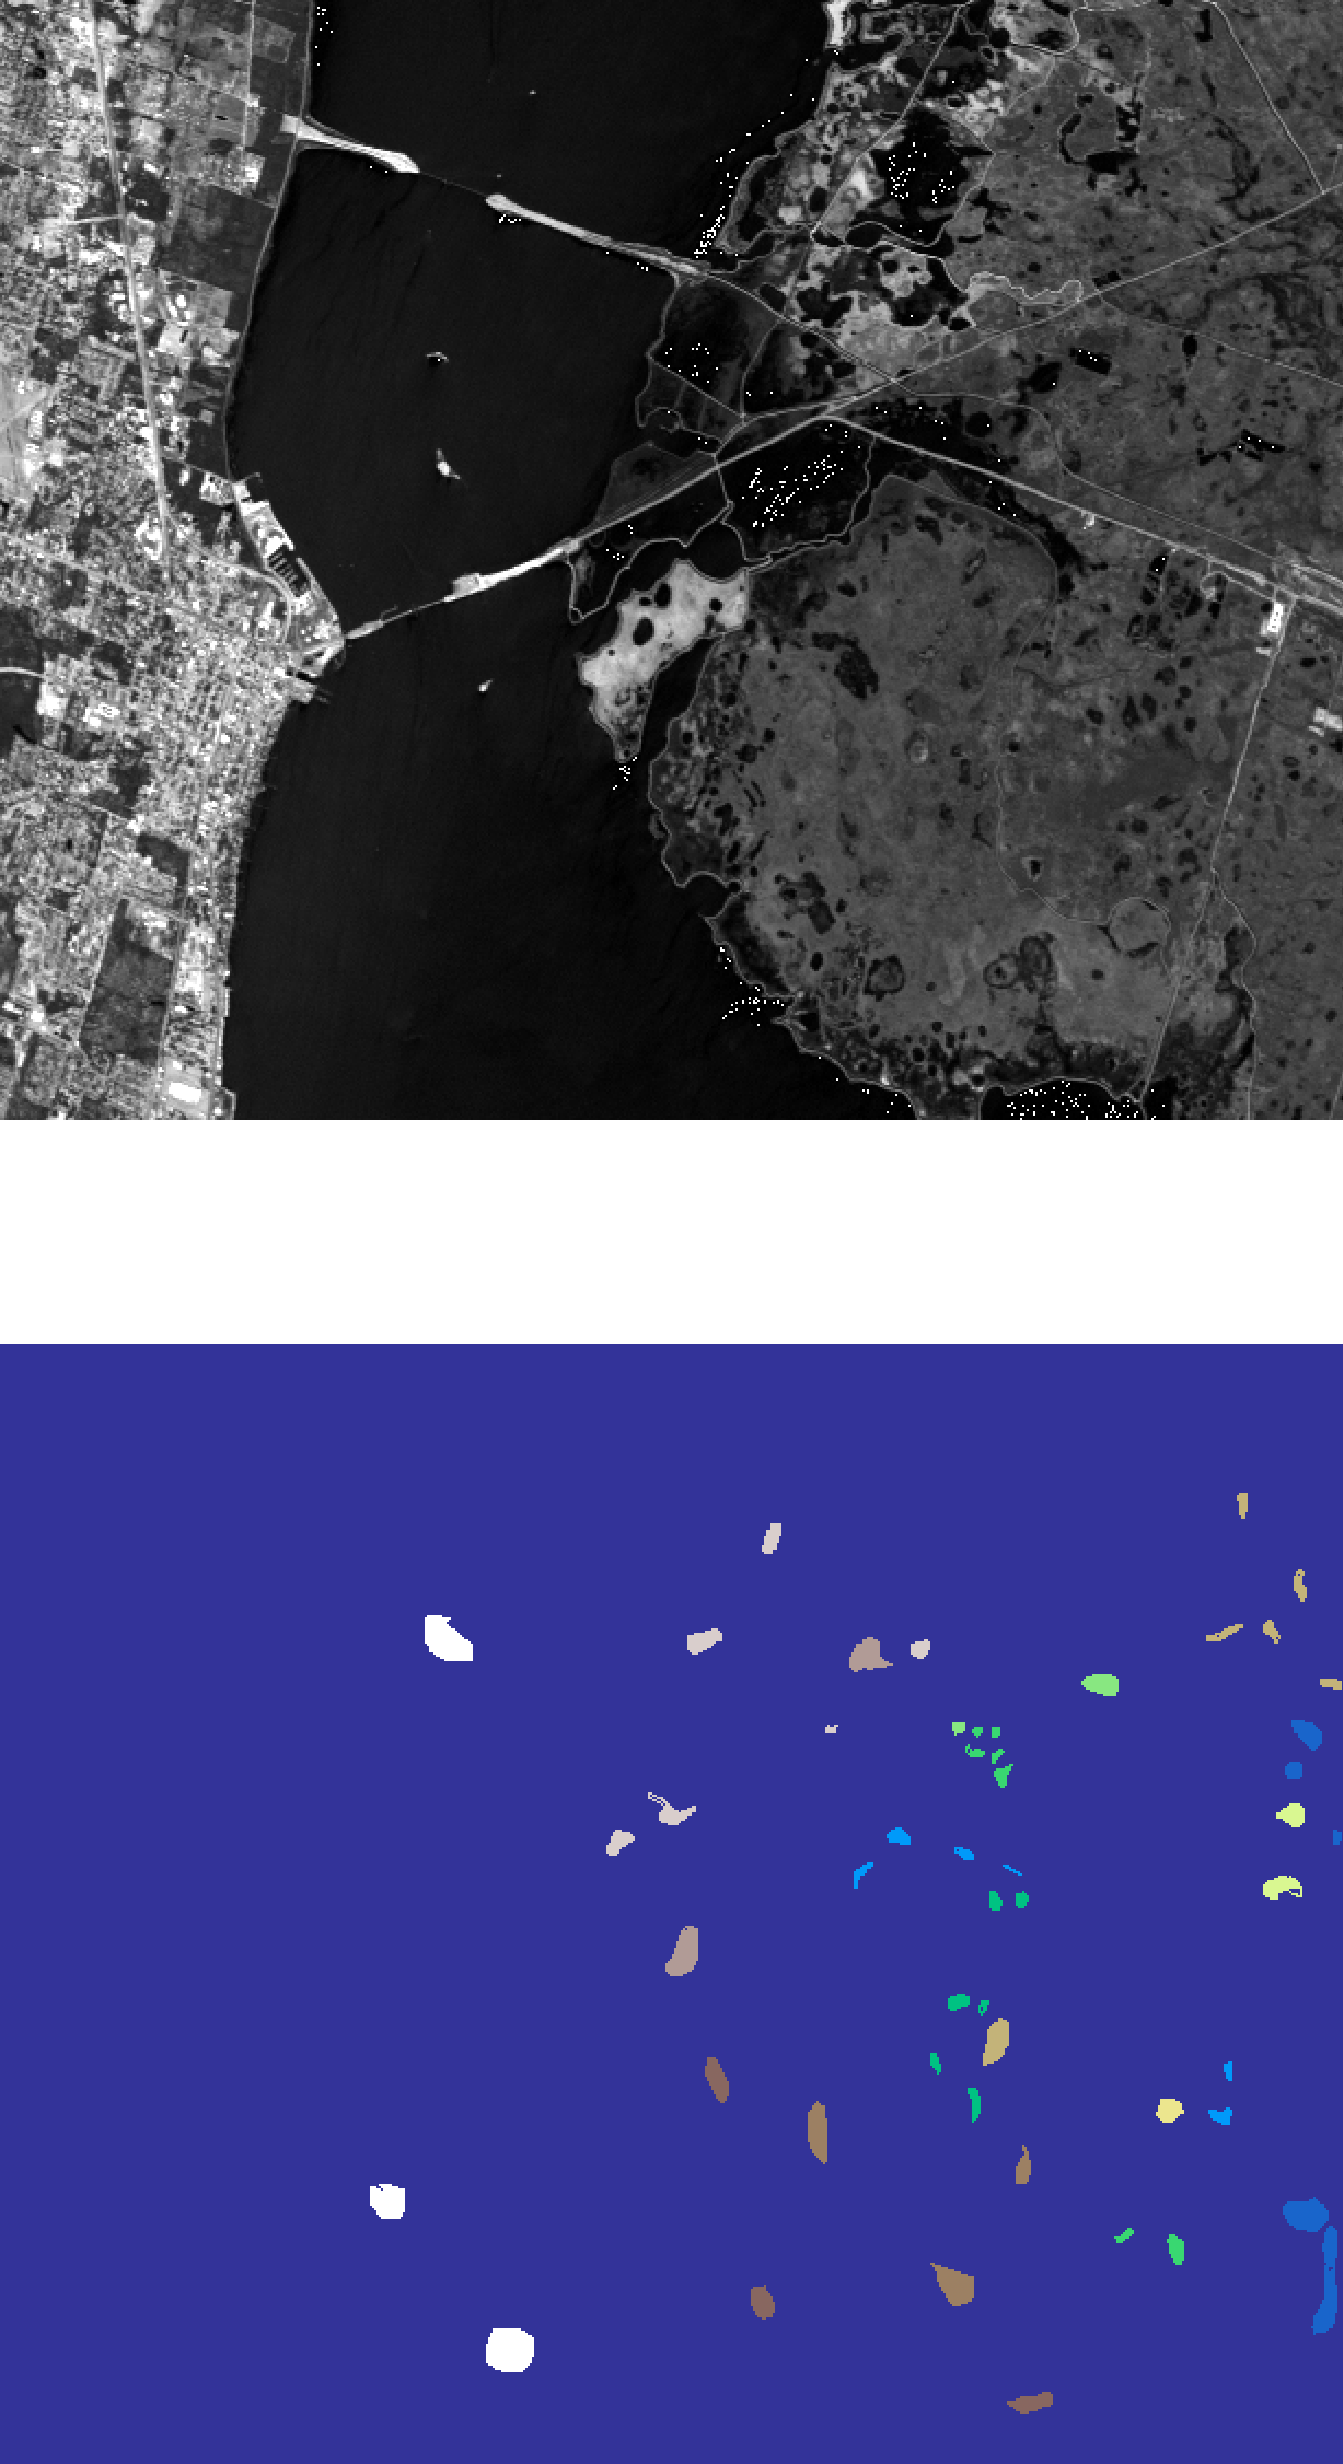
\includegraphics[height=1.5\linewidth]{kennedy_space_center}
		\subcaption{{\medbreak}}\label{fig:kennedy_space_center}
	\end{subfigure}

	\begin{subfigure}{.24\textwidth}
		\centering
		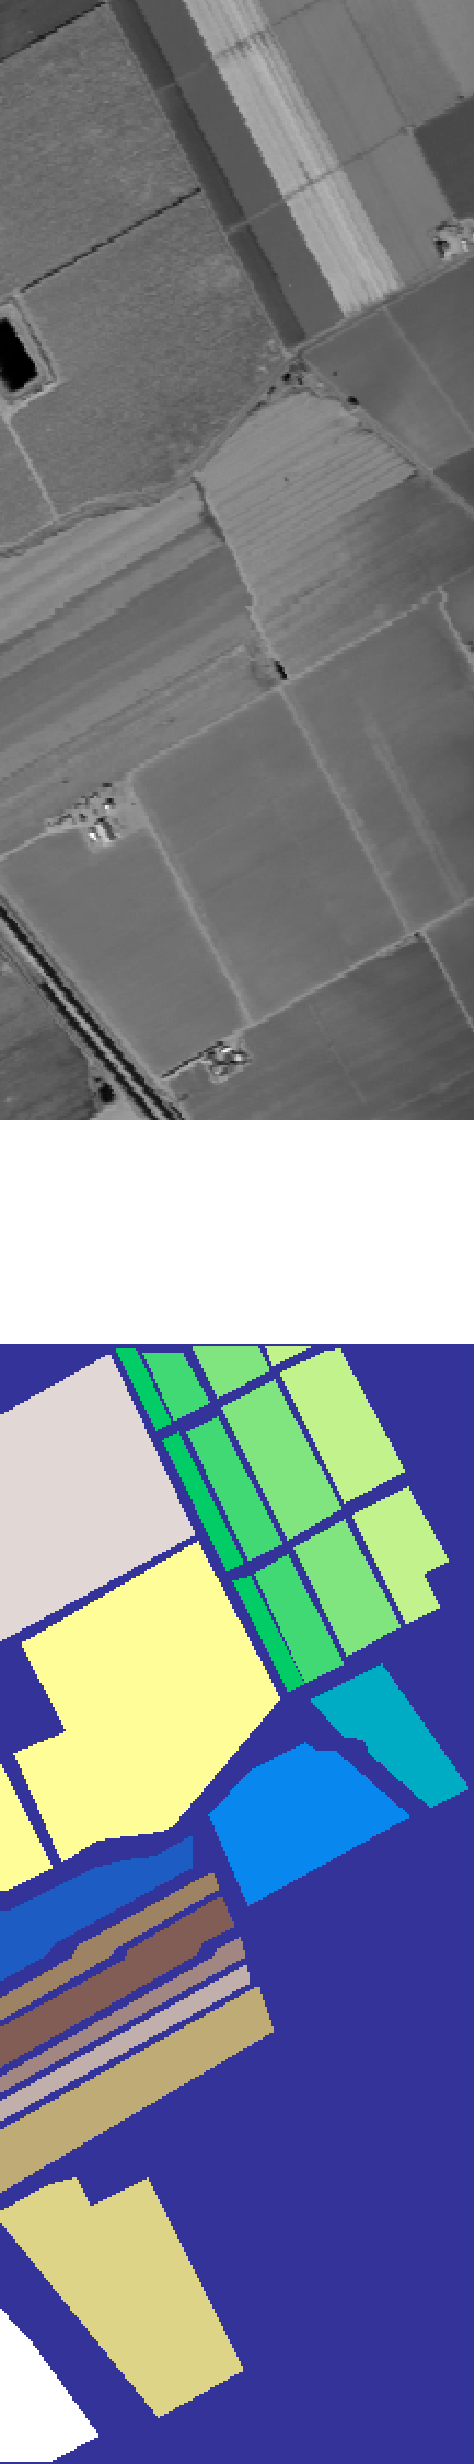
\includegraphics[height=1.5\linewidth]{salinas}
		\subcaption{{\medbreak}}\label{fig:salinas}
	\end{subfigure}
	\begin{subfigure}{.24\textwidth}
		\centering
		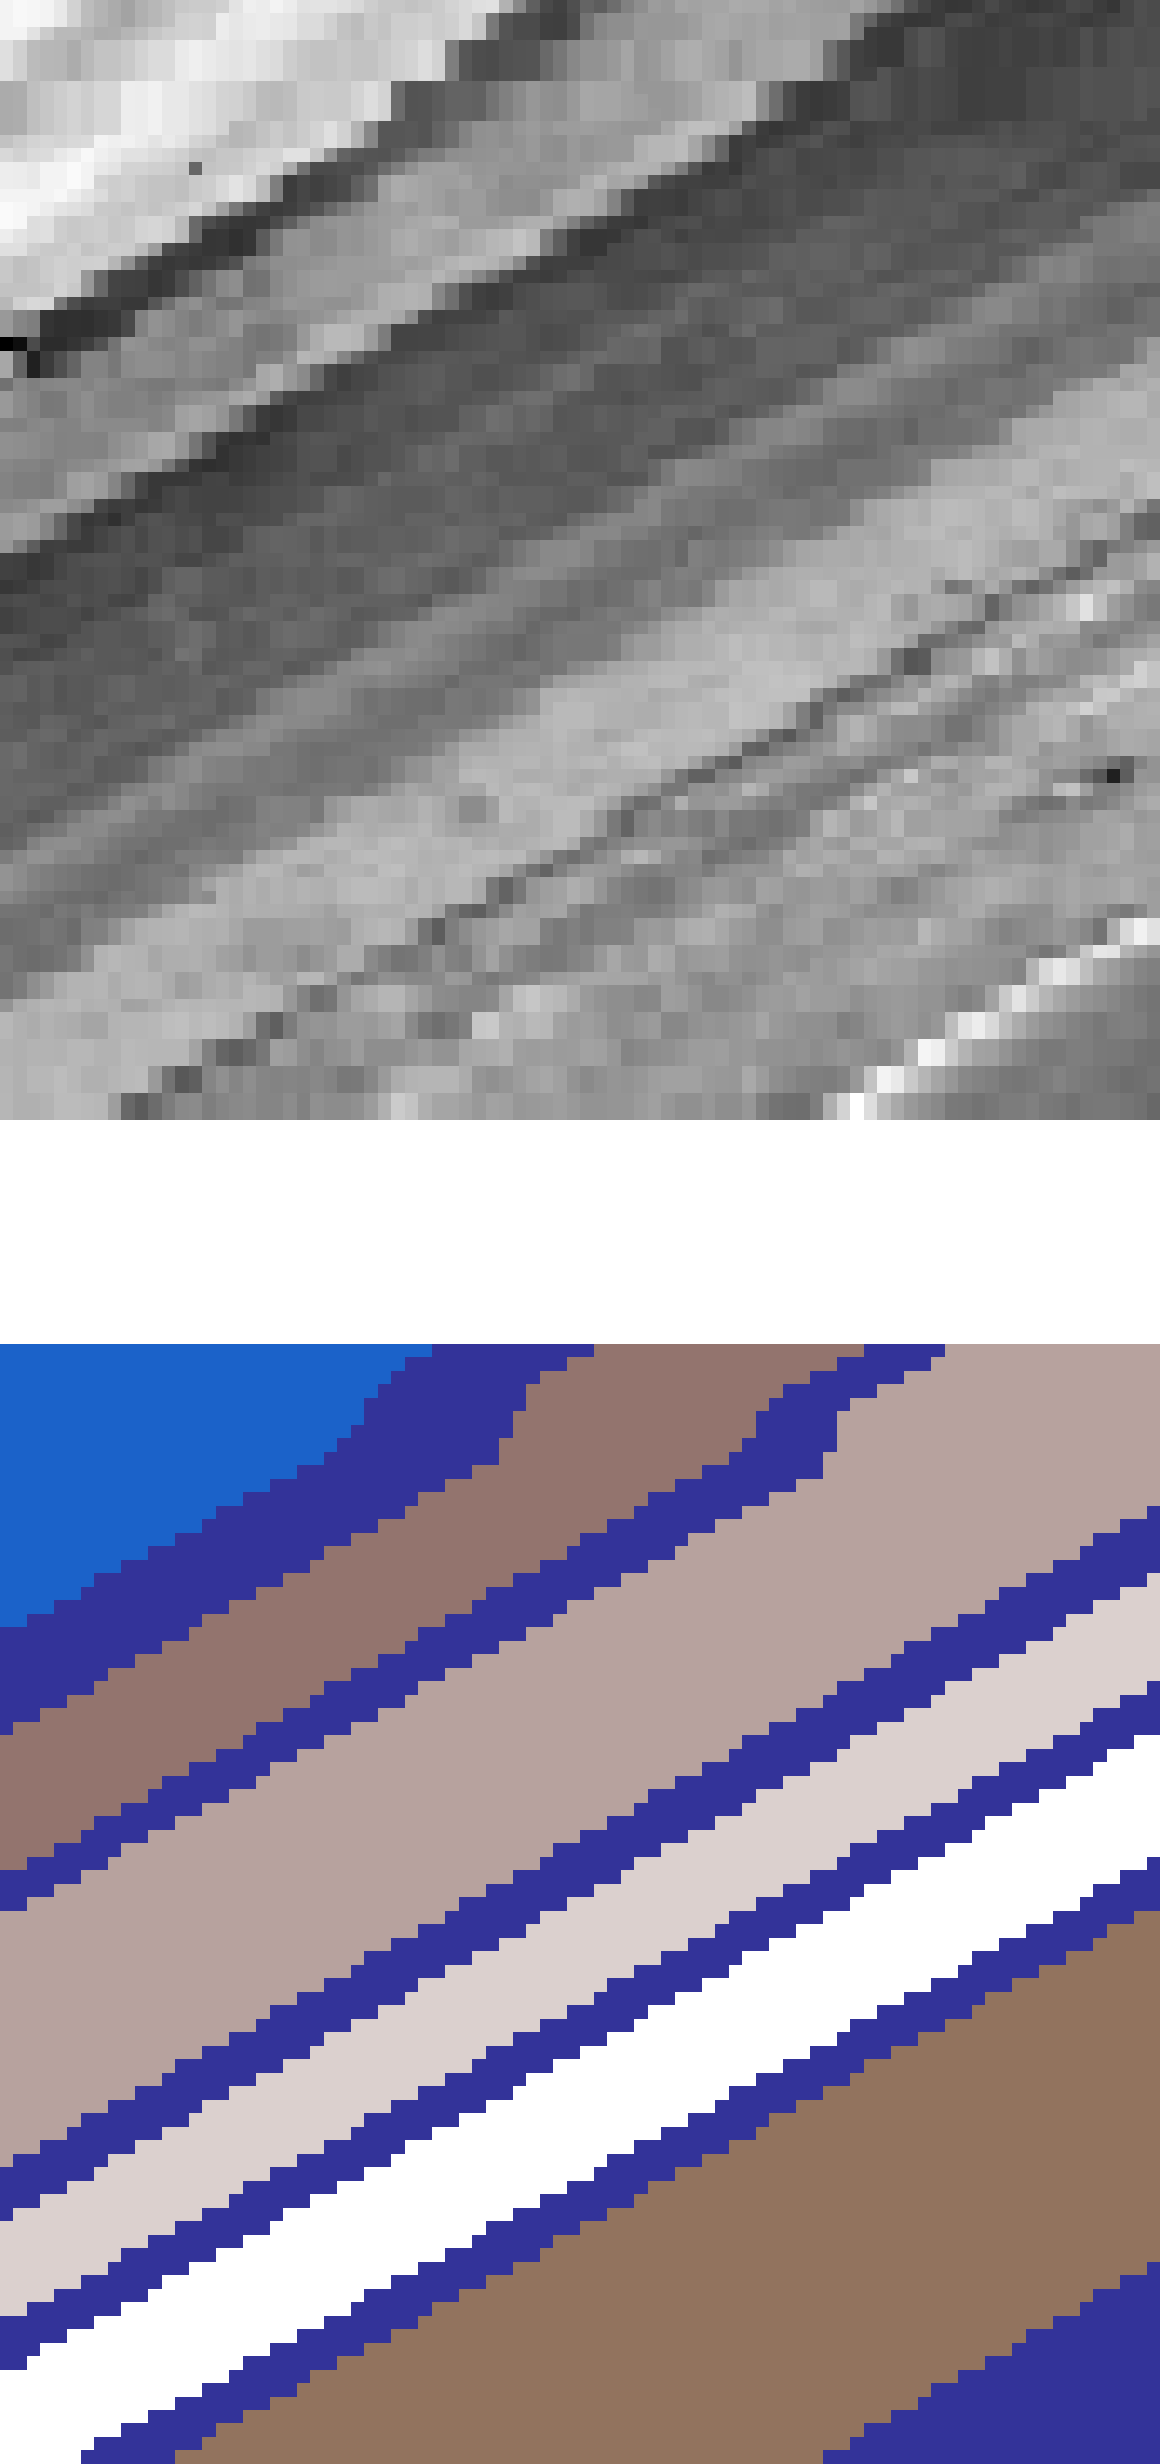
\includegraphics[height=1.5\linewidth]{salinas_a}
		\subcaption{{\medbreak}}\label{fig:salinas_a}
	\end{subfigure}
    \begin{subfigure}{.24\textwidth}
		\centering
		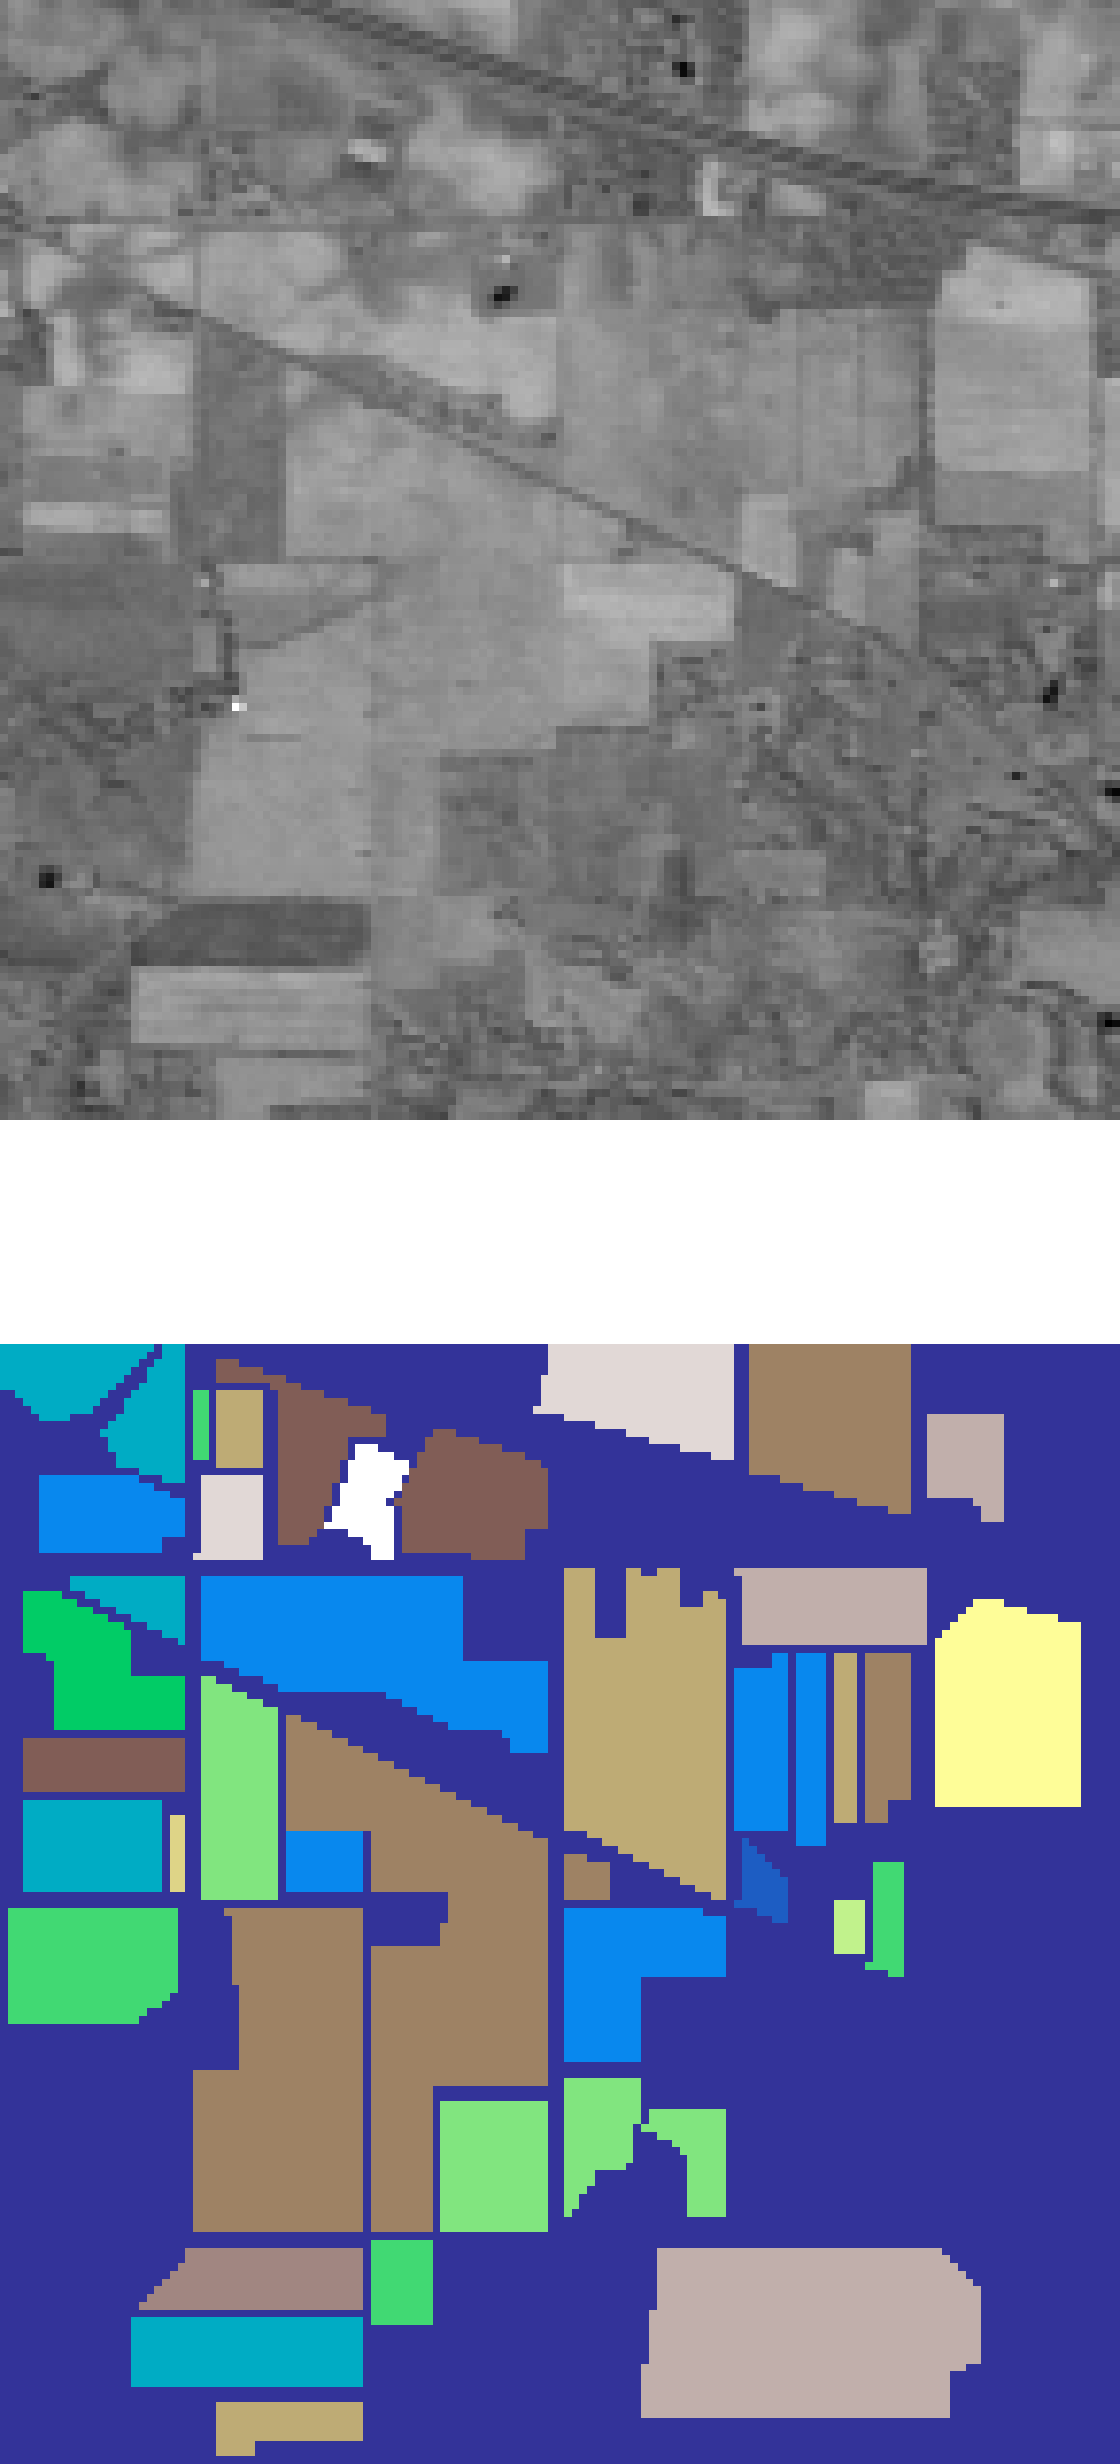
\includegraphics[height=1.5\linewidth]{indian_pines}
		\subcaption{{\medbreak}}\label{fig:indian_pines}
	\end{subfigure}
    \caption[Gray scale visualization of a band and ground truth
    of each scene used in this study.]{Gray scale visualization of a band (top
        row) and ground truth (bottom row) of each scene used in this study.
        (a) Botswana, (b) Pavia Center, (c) Pavia University, (d) Kennedy
        Space Center, (e) Salinas, (f) Salinas A, (g) Indian Pines.
    }~\label{fig:scenes_lulc}
	
\end{figure}

\subsection{Machine Learning Algorithms}

To assess the quality of the K-means SMOTE algorithm,
three other oversampling algorithms were used for benchmarking. ROS and SMOTE
were chosen for their simplicity and popularity. B-SMOTE chosen as a popular
variation of the SMOTE algorithm. We also include the classification results
of no oversampling (NONE) as a baseline.

To assess the performance of each oversampler, we use the classifiers Logistic
Regression (LR) \cite{Nelder1972}, K-Nearest Neighbors (KNN)
\cite{Cover1967} and Random Forest (RF)
\cite{Liaw2002}. This choice was based on the classifiers' popularity for LULC
classification, learning type and training time
\cite{Maxwell2018,Gavade2019}. Since this is a multinomial classification
task, for the LR classification we adopted a one-versus-all approach for each
label. The predicted label is assigned according to the class predicted with
highest probability.

\subsection{Evaluation Metrics}~\label{sec:evaluation-metrics-kmeans}

Most of the satellite-based LULC classification studies (nearly 80\%) employ
\textit{Overall Accuracy} (OA) and the \textit{Kappa Coefficient}
\cite{Gavade2019}. Although, some authors argue that both evaluation metrics,
even when used simultaneously, are insufficient to fully address the area
estimation and uncertainty information needs \cite{Olofsson2013,Pontius2011}.
Other metrics like User's Accuracy (or \textit{Precision}) and Producer's
Accuracy (or \textit{Recall}) are also common metrics to evaluate per-class
prediction power. These metrics consist of ratios employing the True and False
Positives (\textit{TP} and \textit{FP}, number of correctly/incorrectly
classified instances of a given class) and True and
False Negatives (\textit{TN} and \textit{FN}, number of correctly/incorrectly
classified instances as not belonging to a given
class). These metrics are formulated as $Precision = \frac{TP}{TP+FP}$ and
$Recall = \frac{TP}{TP+FN}$. While metrics like OA and \textit{Kappa
Coefficient} are significantly affected by imbalanced class distributions,
\textit{F-Score} is less sensitive to data imbalance and a more appropriate
choice for performance evaluation \cite{Jeni2013}.

The datasets used present significantly high IRs (see Table
\ref{tab:datasets_description_kmeans}). Therefore, it is especially important to
attribute equal importance to the predictive power of all classes, which does
not happen with OA and \textit{Kappa Coefficient}. In this study, we employ 3
evaluation metrics: 1) \textit{G-mean}, since it is not affected by skewed class
distributions, 2) \textit{F-Score}, as it proved to be a more appropriate metric
for this problem when compared to other commonly used metrics \cite{Jeni2013},
and 3) \textit{Overall Accuracy}, for discussion purposes.

\begin{itemize}
    \item The \textit{G-mean} consists of the geometric mean of $Specificity =
        \frac{TN}{TN + FP}$ and \textit{Sensitivity} (also known as
        \textit{Recall}). For multiclass problems, The \textit{G-mean} is
        expressed as:

        $$\textit{G-mean} = \sqrt{ \overline{Sensitivity} \times
        \overline{Specificity}}$$

    \item \textit{F-score} is the harmonic mean of \textit{Precision} and
        \textit{Recall}. The \textit{F-score} for the multi-class case can be
        calculated using their average per class values \cite{He2009}:

          $$\textit{F-score}=2\frac{\overline{Precision} \times
          \overline{Recall}}{\overline{Precision} + \overline{Recall}}$$

    \item \textit{Overall Accuracy} is the number of correctly classified
        instances divided by the total amount of instances. Having \( c \) as
        the label of the various classes, \textit{Accuracy} is given by the
        following formula:

          $$\textit{Accuracy} = \frac{ \sum\limits_{c}{ \text{TP}_{c} } }{
          \sum\limits_{c}{ (\text{TP}_{c}  + \text{FP}_{c}) } } $$

\end{itemize}

In the case of \textit{G-mean} and \textit{F-score}, both metrics are computed
for each label and their unweighted mean is calculated (\textit{i.e.},
following a ``macro'' approach). In this study we assume that all labels
have an equivalent importance for the classification task.

\subsection{Experimental Procedure}

The procedure for the experiment started with the definition of a
hyperparameter search grid, where a list of possible values for each relevant
hyperparameter in both classifiers and oversamplers is stored. Based on this
search grid, all possible combinations of oversamplers, classifiers and
hyperparameters are formed.  Finally, for each dataset, hyperparameter
combination and initialization we use the evaluation strategy shown in Figure
\ref{fig:experiment_pipeline}: $k$-fold cross-validation strategy where $k=5$
to train each model defined and save the averaged scores of each split.

In the 5-fold cross validation strategy, a combination
of oversampler, classifier and hyperparameters vector is fit 5 times
per dataset. Before the training
phase, the training set
(containing $\frac{4}{5}$ of the dataset) is oversampled using one of the methods
described (except for the baseline method NONE), creating an augmented
dataset with the exact same number of instances for
each class. The newly formed training dataset is used to train the classifier
and the test set ($\frac{1}{5}$ of the dataset)
is used to evaluate the performance of the classifier. The evaluation scores
are then averaged over the 5 times the process is repeated. The range of
hyperparameters used are shown in table \ref{tab:grid_kmeans}. The definition of
hyperparameters for the K-means SMOTE oversampler is defined according to the
recommendations discussed in the original K-means SMOTE
paper~\cite{Douzas2018}.

\begin{figure}
	\centering
	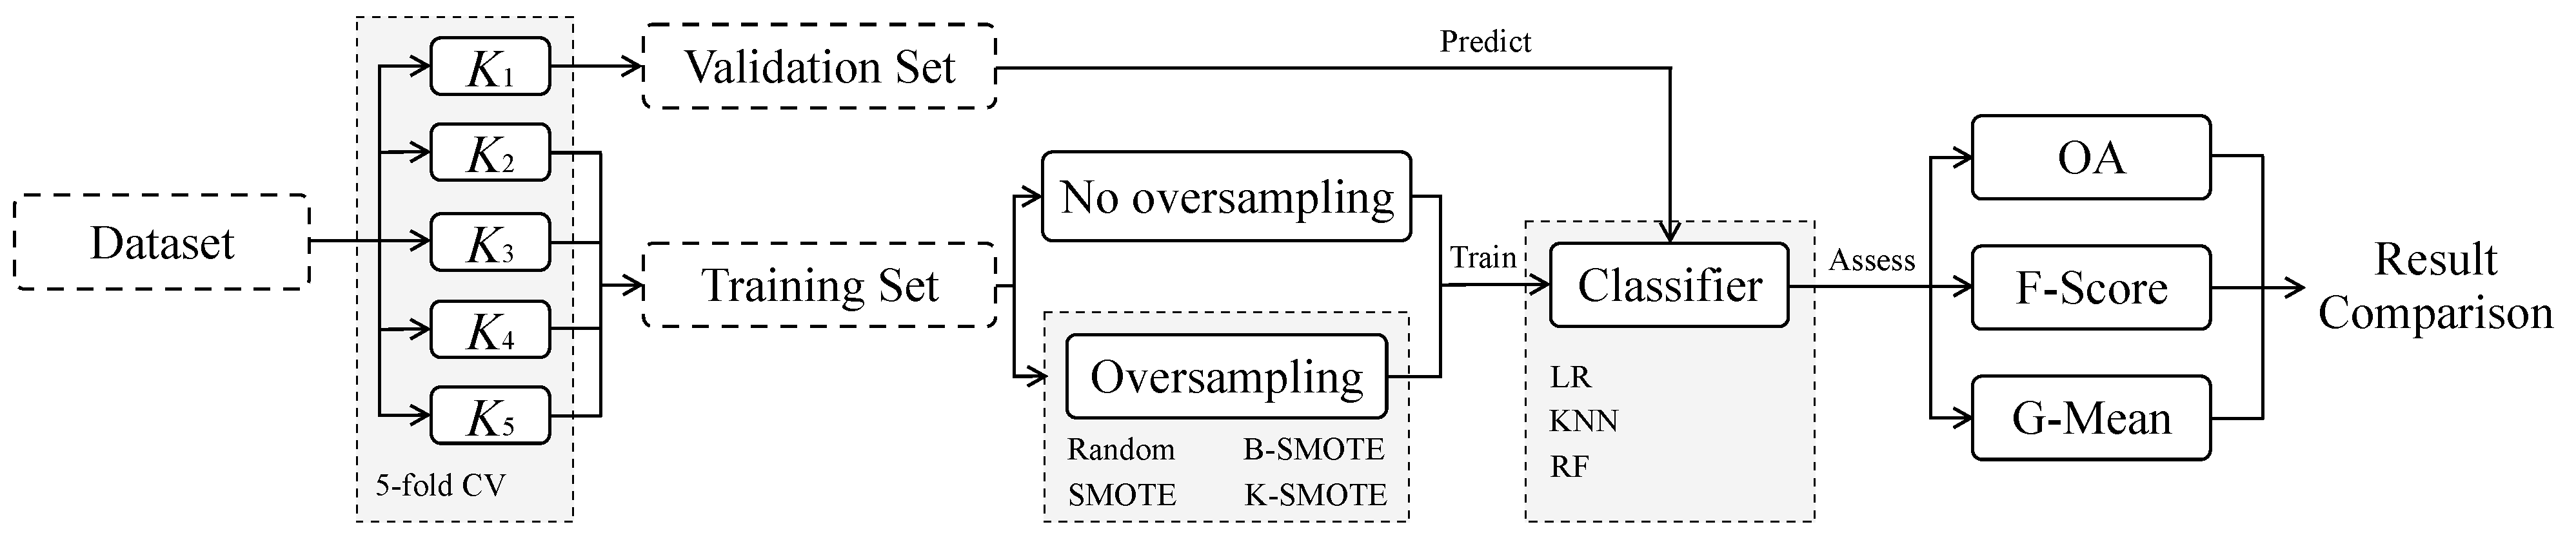
\includegraphics[width=1\linewidth]{experiment_pipeline}
    \caption[Experimental procedure.]{Experimental procedure. The performance metrics are averaged over
        the 5 folds across each of the 3 different initializations of this
        procedure for a given combination of oversampler, classifier and
        hyperparameter definition.
    }~\label{fig:experiment_pipeline}
\end{figure}

\begin{table}
	\centering
    \begin{tabular}{lll}
		\toprule
		Classifier       & Hyperparameters      & Values                            \\
		\midrule
		LR               & maximum iterations   & 10000                             \\
		KNN              & \# neighbors  & {3, 5, 8}                            \\
		RF               & maximum depth        & {None, 3, 6}                      \\
		                 & \# estimators & {50, 100, 200}                         \\
		\toprule
		Oversampler      &                      &                                   \\
		\midrule
        K-means SMOTE    & \# neighbors  & {3, 5}                            \\
		                 & \# clusters (as \% of number of instances)   & {1$^*$, 0.1, 0.3, 0.5, 0.7, 0.9}      \\
                         & Exponent of mean distance & {auto, 2, 5, 7}       \\
                         & IR threshold  & {auto, 0.5, 0.75, 1.0}            \\
		SMOTE            & \# neighbors  & {3, 5}                            \\
		BORDERLINE SMOTE & \# neighbors  & {3, 5}                            \\
		\bottomrule
	\end{tabular}
    \caption[Hyper-parameters grid.]{Hyper-parameters grid. $^*$~One cluster is generated in total, a
    corner case that mimics the behavior of SMOTE
    }\label{tab:grid_kmeans}
\end{table}

\subsection{Software Implementation}~\label{sec:implementation-kmeans}

The experiment was implemented using the Python programming language, using the
\href{https://scikit-learn.org/stable/}{Scikit-Learn}~\cite{Pedregosa2011},
\href{https://imbalanced-learn.org/en/stable/}{Imbalanced-Learn}~\cite{JMLR:v18:16-365},
\href{https://geometric-smote.readthedocs.io/en/latest/?badge=latest}{Geometric-SMOTE},
\href{https://cluster-over-sampling.readthedocs.io/en/latest/?badge=latest}{Cluster-Over-Sampling}
and \href{https://research-learn.readthedocs.io/en/latest/?badge=latest}{Research-Learn} libraries.
All functions, algorithms, experiments and results are provided at the
\href{https://github.com/joaopfonseca/publications}{GitHub
repository of the project}.

\section{Results \& Discussion}~\label{sec:results-kmeans}

When evaluating the performance of an algorithm across multiple datasets, it
is generally recommended to avoid direct score comparisons and use
classification rankings instead~\cite{Demsar2006}. This is done by assigning
a ranking to oversamplers based on the different combinations of classifier,
metric and dataset used. These rankings are also used for the statistical
analyses presented in Section~\ref{sec:statistical_analysis-kmeans}.

The rank values are assigned based on the mean validation scores resulting
from the experiment described in Section~\ref{sec:methodology-kmeans}. The averaged
ranking results are computed over 3 different initialization seeds and a 5
fold cross validation scheme, returning a real number within the interval
$[1,5]$.

The hyperparameter optimization ensures that both oversamplers and classifiers
are well adapted to each of the datasets used in the experiment. Specifically,
the optimization of classifiers' hyperparameters is not particularly relevant
since our focus is to study the relative performance scores across
oversamplers. This will provide insights on the quality of the artificial data
generated by each oversampler. The classifiers' hyperparameter tuning was done
to avoid the over/underfitting of classifiers, since they are trained on the same
data subsets along with artificial data generated with different methods.

\subsection{Results}

The mean ranking of oversamplers is presented in
Figure~\ref{fig:mean_sem_ranking}. This ranking was computed by averaging the
ranks of the mean cross-validation scores per dataset, oversampler and
classifier. K-means SMOTE achieves the best mean ranking across datasets with
low standard deviation.


\begin{figure}
    \centering
	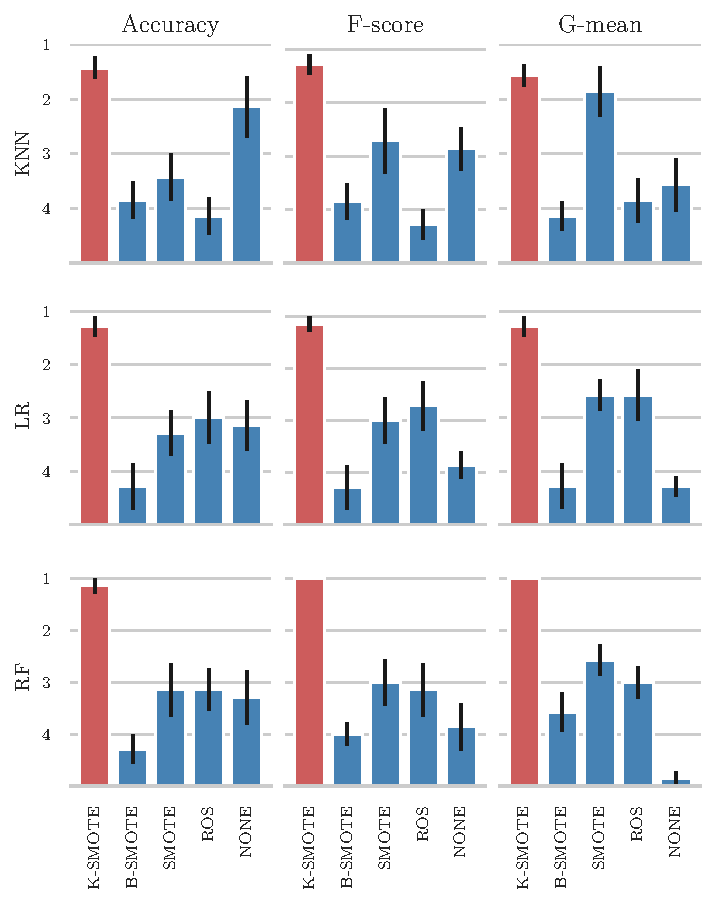
\includegraphics[width=.65\linewidth]{mean_rankings_bar_chart}
	\caption{%
    	Results for mean ranking of oversamplers across datasets.
    }~\label{fig:mean_sem_ranking}
\end{figure}

The mean cross-validation scores are shown in Table~\ref{tab:mean_sem_scores}.
As discussed previously in this section, the disparity of performance levels
across datasets makes the analysis of these scores less informative.

\begin{table}
	\centering
    \addtolength{\leftskip} {-2cm}
    \addtolength{\rightskip}{-2cm}
    \pgfplotstabletypeset[
        col sep=comma,
        string type,
        every head row/.style={%
            before row=\toprule,
            after row=\midrule
        },
        every last row/.style={after row=\bottomrule},
        string type,
    ]{figures/kmeans-smote-lulc/mean_sem_scores.csv}
    \caption{%
    	Mean cross-validation scores of oversamplers.
    }~\label{tab:mean_sem_scores}
\end{table}

The mean cross-validation scores for each dataset are presented in
Table~\ref{tab:cross_validation_scores} (see appendix). This table allows the direct
comparison of the performance metrics being analysed.

\subsection{Statistical Analysis}~\label{sec:statistical_analysis-kmeans}

The experiment's multi-dataset context was used to perform a Friedman
test~\cite{Friedman1937}. Table~\ref{tab:friedman_test_kmeans} shows the results
obtained in the Friedman test performed, where the null hypothesis is rejected
in all cases. The rejection of the null hypothesis implies that the
differences between the differences among the different oversamplers are not
random, in other words, these differences are statistically significant.

\begin{table}[ht]
    \centering
    \pgfplotstabletypeset[
        col sep=comma,
        string type,
        every head row/.style={%
            before row=\toprule,
            after row=\midrule
        },
        every last row/.style={after row=\bottomrule},
        string type,
    ]{figures/kmeans-smote-lulc/friedman_test.csv}
    \caption[Results for Friedman test.]{%
        Results for Friedman test. Statistical significance is tested at a
        level of $\alpha = 0.05$. The null hypothesis is that there is no
        difference in the classification outcome across oversamplers.
    }~\label{tab:friedman_test_kmeans}
\end{table}

A Wilcoxon signed-rank test \cite{Wilcoxon1945} was also performed to
understand whether K-means SMOTE's superiority was statistically significant
across datasets and oversamplers, as suggested in \cite{Demsar2006}. This
method is used as an alternative to the paired Student's t-test, since the
distribution of the differences between the two samples cannot be assumed as
normally distributed. The null hypothesis of the test is that K-means SMOTE's
performance is similar to the compared oversampler (i.e., the oversamplers
used follow a symmetric distribution around zero).

\begin{table}
    \centering
    \pgfplotstabletypeset[
        col sep=comma,
        string type,
        every head row/.style={%
            before row=\toprule,
            after row=\midrule
        },
        every last row/.style={after row=\bottomrule},
        string type,
    ]{figures/kmeans-smote-lulc/wilcoxon_test.csv}
    \caption[\textit{p-values} of the Wilcoxon signed-rank test.]{%
        \textit{p-values} of the Wilcoxon signed-rank test. Boldface values
        are statistically significant at a significance level of $\alpha =
        0.05$.
    }~\label{tab:wilcoxon_test_kmeans}
\end{table}

\subsection{Discussion}

The mean rankings presented in
Figure~\ref{fig:mean_sem_ranking} show that on average,
K-means SMOTE produced the best results for every classifier and performance
metric used. This is due to the clustering phase and subsequent selection of
data to be considered for oversampling. By successfully clustering and
selecting the relevant areas in the data space to oversample, the generation
of artificial instances is done only in the context of minority regions that
represent well their spectral signature.

As previously discussed, the direct comparison of performance metrics averaged
over various datasets is not recommended due to the varying levels of
performance of classifiers across datasets~\cite{Demsar2006}. Nonetheless,
these results are shown in Table~\ref{tab:mean_sem_scores} to provide a fuller
picture of the results obtained in the experiment. We found that on average
K-means SMOTE provides increased performance, regardless of the classifier and
performance metric used. More importantly, K-means SMOTE guaranteed a more
consistent performance across datasets and with less variability, which can be
attested in Figure~\ref{fig:mean_sem_ranking} and
Tables~\ref{tab:mean_sem_scores} and~\ref{tab:cross_validation_scores}.

As discussed in Subsection~\ref{sec:evaluation-metrics-kmeans}, Evaluation Metrics,
our results are consistent with the findings in~\cite{Olofsson2013,
Pontius2011}. Particularly, we consider the results obtained in our experiment
using Overall Accuracy to be less informative than the results obtained with
the remaining performance metrics, since this metric is affected by imbalanced
class distributions. The majority class bias in this metric can be observed in
our experiment in Figure~\ref{fig:mean_sem_ranking} with the
classifiers LR and KNN, where the control method (NONE) is only outperformed
by K-means SMOTE. This effect is observed with more detail in
Table~\ref{tab:mean_sem_scores}, where the benchmark oversamplers are
outperformed by the control method in 16 out of 63 tests (approximately 25\%).
Out of these, most refer to tests using overall accuracy among the four
datasets with highest IR, showing the overall accuracy's class imbalance bias
discussed in~\cite{Olofsson2013, Pontius2011}. The K-means SMOTE oversampler
is only outperformed by the control method in 3 of tests (all of them using
overall accuracy). This is an improvement over the benchmark oversamplers,
showing that generally K-means SMOTE is the best choice even when overall
accuracy is used as the main performance metric.

In the majority of the cases, K-means SMOTE was able to generate higher
quality data due to the non-random selection of data spaces to oversample.
This can be seen in the performance of the classifiers trained on top of this
data generation step, making it a more informed data generation method in the
context of LULC\@.

The performance of both oversamplers and classifiers is generally dependent on
the dataset being used. Although both absolute and relative scores between the
different oversamplers are dependent on the choice of metric and classifier,
K-means SMOTE's relative performance is consistent across datasets and
generally outperforms the remaining oversampling methods in 56 of the 63 tests
(approximately 89\%). The mean cross-validation results found in
Table~\ref{tab:cross_validation_scores} show that performance-wise, K-means
SMOTE is always better than or as good as SMOTE, with the exception of 4
situations (representing 6\% of the tests done), in which cases the percentage
point difference is neglectable ($\leq 0.1$ percentage points). 

The statistical tests showed that not only there is a statistically
significant difference across the oversamplers used in this problem (found in
the Friedman test presented in Table~\ref{tab:friedman_test_kmeans}), but also that
K-means SMOTE's superior performance is statistically significant at a level
of 0.05 in 27 out of 28 tests in the Wilcoxon signed-rank test shown in
Table~\ref{tab:wilcoxon_test_kmeans} (approximately 96\% of the tests performed).
This shows that, in most cases, the usage of k-Means SMOTE improves the
quality of LULC classification when compared to using SMOTE in its original
format, which remains the most popular oversampler among the remote sensing
community.

Although the usage of K-means SMOTE successfully captured the spectral
signatures of the minority classes, it was done using K-means, a
problem-agnostic clusterer. Consequently, the implementation of this method
using a GIS-specific clusterer that considers the geographical traits of
different regions (e.g., using the sampled pixels' geographical coordinates),
may be a promising direction towards the development of more appropriate
oversampling techniques in the remote sensing domain.

\section{Conclusion}~\label{sec:conclusion-kmeans} 

This research paper was motivated by the challenges faced when classifying
rare classes for LULC mapping. Cluster-based oversampling is especially useful
in this context because the spectral signature of a given class often varies,
depending on its geographical distribution and the time period within which
the image was acquired. This induces the representation of minority classes as
small clusters in the input space. As a result, training a classifier capable
of identifying LULC minority classes in the hyper/multi-spectral scene over
different areas or periods becomes particularly challenging. The clustering
procedure, performed before the data generation phase, allows for a more
accurate generation of minority samples, as it identifies these minority
clusters.

A number of existing methods to address the imbalanced learning problem were
identified and their limitations discussed. Typically, algorithm-based
approaches and cost-sensitive solutions are not only difficult to implement,
but they are also context dependent. In this paper we focused on oversampling
methods due to their widespread usage, easy implementation and flexibility.
Specifically, this paper demonstrated the efficacy of a recent oversampler,
K-Means SMOTE, applied in a multi-class context for Land Cover Classification
tasks. This was done with sampled data from seven well known and naturally
imbalanced benchmark datasets: Indian Pines, Pavia Center, Pavia University,
Salinas, Salinas A, Botswana and Kennedy Space Center. For each combination of
dataset, oversampler and classifier, the results of every classification task
was averaged across a 5 fold stratification strategy with 3 different
initialization seeds, resulting in a mean validation score of 15
classification tasks. The mean validation score of each combination was then
used to perform the analyses presented in this report.

In 56 out of 63 classification tasks (approximately 89\%), K-means SMOTE led
to better results than ROS, SMOTE, B-SMOTE and no oversampling. More
importantly, we found that K-Means SMOTE is always better or equal than the
second best oversampling method.  K-means SMOTE's performance was independent
from both the classifier and performance metric under analysis. In general,
K-means SMOTE shows a higher performance among the non tree-based classifiers
employed (LR and KNN) when compared with the remaining oversamplers, where
these oversamplers generally failed to improve the quality of classification.
Although these findings are case dependent, they are consistent with the
results presented in~\cite{Douzas2018}. The proposed method also had the most
consistent results across datasets, since it produced the lowest standard
deviations across datasets in 7 out of 9 cases for both analyses, either based
on ranking or mean cross-validation scores.

The proposed algorithm is a generalization of the original SMOTE algorithm. In
fact, the SMOTE algorithm represents a corner case of K-means SMOTE i.e., when
the number of clusters equals to 1. Its data selection phase differs from the
one used in SMOTE and Borderline SMOTE, providing artificially augmented
datasets with less noisy data than the commonly used methods. This allows the
training of classifiers with better defined decision boundaries, especially in
the most important regions of the data space (the ones populated by a higher
percentage of minority class instances).

As stated previously, the usage of this oversampler is technically simple. It
can be applied to any classification problem relying on an imbalanced dataset,
alongside any classifier. K-means SMOTE is available as an open source
implementation for the Python programming language (see
Subsection~\ref{sec:implementation-kmeans}).  Consequently, it can be a useful tool
for both remote sensing researchers and practitioners.

\textbf{This chapter was published as:} Fonseca, J., Douzas, G., Bacao, F.
(2021). Improving Imbalanced Land Cover Classification with K-Means SMOTE:
Detecting and Oversampling Distinctive Minority Spectral Signatures.
Information, 12(7), 266.  https://doi.org/10.3390/info12070266


\chapter{%
    Increasing the Effectiveness of Active Learning: Introducing Artificial
    Data Generation in Active Learning for Land Use/Land Cover
    Classification
}~\label{chp:al-generator-lulc}


\graphicspath{{figures/al-generator-lulc/}}

\begin{adjustwidth}{30pt}{30pt}

    In remote sensing, Active Learning (AL) has become an important technique
    to collect informative ground truth data ``on-demand'' for supervised
    classification tasks. In spite of its effectiveness, it is still
    significantly reliant on user interaction, which makes it both expensive
    and time consuming to implement. Most of the current literature focuses on
    the optimization of AL by modifying the selection criteria and the
    classifiers used. Although improvements in these areas will result in more
    effective data collection, the use of artificial data sources to reduce
    human-computer interaction remains unexplored. In this paper, we introduce
    a new component to the typical AL framework, the data generator, a source
    of artificial data to reduce the amount of user-labeled data required in
    AL\@. The implementation of the proposed AL framework is done using
    Geometric SMOTE as data generator. We compare the new AL framework to the
    original one using similar acquisition functions and classifiers over
    three AL-specific performance metrics in seven benchmark datasets. We show
    that this modification of the AL framework significantly reduces cost and
    time requirements for a successful AL implementation in all of the
    datasets used in the experiment. 

\end{adjustwidth}

\vspace{.5cm}
\textbf{Keywords:} Active Learning; Artificial Data Generation; Land Use/Land Cover Classification;  Oversampling; SMOTE

\section{Introduction}~\label{sec:introduction-al-generator}

The technological development of air and spaceborne sensors, as well as the
increasing number of remote sensing missions have allowed the continuous
collection of large amounts of high quality remotely sensed data. This data is
often composed of multi and hyper spectral satellite imagery, essential for
numerous applications, such as Land Use/Land Cover (LULC) change detection,
ecosystem management~\cite{Nagai2020}, agricultural
management~\cite{Huang2018}, water resource management~\cite{Wang2018}, forest
management, and urban monitoring~\cite{Khatami2016}. Despite LULC maps being
essential for most of these applications, their production is still a
challenging task~\cite{Gavade2019, Wulder2018}. They can be updated using one
of the following strategies:

\begin{enumerate}
    \item Photo-interpretation. This approach consists of evaluating a patch's
        LULC class by a human operator based on orthophoto and satellite image
        interpretation~\cite{costa2020introducing}. This method guarantees a
        decent level of accuracy, as it is dependent on the interpreter's
        expertise and human error. Typically, it is an expensive,
        time-consuming task that requires the expertise of a
        photo-interpreter. This task is also frequently applied to obtain
        ground-truth labels for training and/or validating Machine Learning
        (ML) algorithms for related tasks~\cite{vermote2020remote,
        COSTANTINO2020}. 
    \item Automated mapping. This approach is based on the usage of a ML
        method or a combination of methods in order to obtain an updated LULC
        map. The development of a reliable automated method is still a
        challenge among the ML and remote sensing community, since the
        effectiveness of existing methods varies across applications and
        geographical areas~\cite{Gavade2019}. Typically, this method requires
        the existence of ground-truth data, which is frequently outdated or
        nonexistent for the required time frame~\cite{Nagai2020}. On the other
        hand, employing a ML method provides readily available and relatively
        inexpensive LULC maps. The increasing quality of state-of-the-art
        classification methods have motivated the application and adaptation
        of these methods in this domain~\cite{Maxwell2018}.
    \item Hybrid approaches. These approaches employ photo-interpreted data to
        augment the training dataset and improve the quality of automated
        mapping~\cite{Ruzicka2020}. It attempts to accelerate the
        photo-interpretation process by selecting a smaller sample of the
        study area to be interpreted. The goal is to minimize the inaccuracies
        found in the LULC map by supplying high-quality ground-truth data to
        the automated method. The final (photo-interpreted) dataset consists
        of only the most informative samples, \textit{i.e.}, patches that are
        typically difficult to classify for a traditional automated mapping
        method~\cite{Liu2020}. 
\end{enumerate}

The latter method is best know as AL\@. It is especially useful whenever there
is a shortage or even absence of ground-truth data and/or the mapping region
does not contain updated LULC maps~\cite{Su2020}. In a context of limited
sample-collection budget, the collection of the most informative samples
capable of optimally increasing the classification accuracy of a LULC map is
of particular interest~\cite{Su2020}. AL attempts to minimize the
human-computer interaction involved in photo-interpretation by selecting the
data points to include in the annotation process. These data points are
selected based on an uncertainty measure and represent the points close to the
decision borders. Afterwards, they are passed on for photo-interpretation and
added to the training dataset, while the points with the lowest uncertainty
values are ignored for photo-interpretation and classification. This process
is repeated until a convergence criterion is reached~\cite{Pasolli2016}. 

The relevant work developed within AL is described in detail in
Section~\ref{sec:al-sota-al-generator}. This paper attempts to address some of the
challenges found in AL, mainly inherited from automated and photo-interpreted
mapping: mapping inaccuracies and time consuming human-computer interactions.
These challenges have different sources:

\begin{enumerate}
    \item Human error. The involvement of photo-interpreters in the data
        labeling step carries an additional risk to the creation of LULC
        patches. The minimum mapping unit being considered, as well as the
        quality of the orthophotos and satellite images being used, are some of
        the factors that may lead to the overlooking of small-area LULC patches
        and label-noisy training data~\cite{Pelletier2017}.
    \item High-dimensional datasets. Although the amount of bands
        (\textit{i.e.}, features) present in multi and hyper spectral images
        contain useful information for automated classification, they also
        introduce an increased level of complexity and redundancy in the
        classification step~\cite{Stromann2020}. These datasets are often
        prone to the Hughes phenomenon, also known as the curse of
        dimensionality. 
    \item Class separability. Producing an LULC map considering classes with
        similar spectral signatures makes them difficult to
        separate~\cite{Alonso-Sarria2019}. A lower pixel resolution of the
        satellite images may also imply mixed-class pixels, which may lead to
        both lower class separability as well as higher risk of human error.
    \item Existence of rare land cover classes. The varying morphologies of
        different geographical regions naturally implies an uneven distribution
        of land cover classes~\cite{Feng2018}. This is particularly relevant in
        the context of AL since the data selection method is based on a given
        uncertainty measure over data points whose class label is unknown.
        Consequently, AL's iterative process of data selection may disregard
        wrongly classified land cover areas belonging to a minority class.
\end{enumerate}

Research developed in the field of AL typically focus on the reduction of
human error by minimizing the human interaction with the process through the
development of more efficient classifiers and selection criteria within the
generally accepted AL framework. Concurrently, the problem of rare land cover
classes is rarely addressed. This is a frequent problem in the ML community,
known as the Imbalanced Learning problem. This problem exists whenever there
is an uneven between-class distribution in the dataset~\cite{Chawla2004}.
Specifically, most classifiers are optimized and evaluted using accuracy-like
metrics, which are designed to work primarily with balanced datasets.
Consequently, these metrics tend to introduce a bias towards the majority
class by attributing an importance to each class proportional to its relative
frequency~\cite{Maxwell2018}. As an example, such a classifier could achieve
an overall accuracy of 99\% on a binary dataset where the minority class
represents 1\% of the overall dataset and still be useless. A number of
methods have been developed to deal with this problem.  They can be
categorized into three different types of
approaches~\cite{Fernandez2013,Kaur2019}.  Cost-sensitive solutions perform
changes to the cost matrix in the learning phase. Algorithmic level solutions
modify specific classifiers to reinforce learning on minority classes.
Resampling solutions modify the training data by removing majority samples
and/or generating artificial minority samples. The latter is independent from
the context and can be used alongside any classifier.  Since we are interested
in the introduction of artificial data generation in AL, we will analyze the
state-of-the-art on resampling techniques (specifically oversampling) in
Section~\ref{sec:ovs-sota-al-generator}.

In this paper, we propose a novel AL framework to address two limitations
commonly found in the literature: minimize human-computer interaction and
reduce the class imbalance bias. This is done with the introduction of an
additional component in the iterative AL procedure (the generator) that
is used to generate artificial data to both balance and augment the training
dataset. The introduction of this component is expected to reduce the number
of iterations required until the classifier reaches a satisfactory
performance.

This paper is organized as follows: Section~\ref{sec:introduction-al-generator} explains
the problem and its context, Sections~\ref{sec:al-sota-al-generator} and~\ref{sec:ovs-sota-al-generator}
describe the state of the art in AL and Oversampling techniques,
Section~\ref{sec:proposed-method-al-generator} explains the proposed method,
Section~\ref{sec:methodology-al-generator} covers the datasets, evaluation metrics, ML
classifiers and experimental procedure, Section~\ref{sec:results-al-generator} presents the
experiment's results and discussion and Section~\ref{sec:conclusion-al-generator} presents
the conclusions drawn from our findings.

\section{Active Learning Approaches}~\label{sec:al-sota-al-generator}

As the amount of unlabeled data increases, the interest and practical
usefulness of AL follows that trend~\cite{Kottke2017}. AL is used as the
general definition of frameworks aiming to train a learning system in multiple
steps, where a set of new data points are chosen and added to the training
dataset each time~\cite{Ruzicka2020}. Typically, an AL framework is composed
of the following elements~\cite{Sverchkov2017,Su2020,Ruzicka2020}:

\begin{enumerate}
    \item Unlabeled dataset. Consists of the original data source (or a sample
        thereof). It is used in combination with the chooser and the selection
        criterion to expand the training dataset in regions where the
        classification uncertainty is higher. Therefore, the unlabeled
        dataset is used for both producing the initial training
        dataset by selecting a set of instances for the
        supervisor to annotate (discussed in point 3) and calculating the
        uncertainty map to augment the training dataset.
    \item Supervisor. A human annotator (or team of human
        annotators) to which the uncertainty map is
        presented to. The supervisor is responsible for annotating unlabeled
        instances to be added to the augmented dataset. In remote sensing, the
        supervisor is typically a photo-interpreter, as is the case
        in~\cite{li2020}. Some of the research also refers to the supervisor
        as the \textit{oracle}~\cite{Ruzicka2020, Yoo2019, Aghdam2019,
        Cawley2011}.
    \item Initial training dataset. It is a small, labeled sample of
        the original data source used to initiate the first AL
        iteration. The size of the initial training sample normally varies
        between no instances at all and 10\% of the unlabeled
        dataset~\cite{Li2013}.
    \item Current and expanded training dataset. It is the concatenation of
        the initial training dataset and the datasets labeled by the
        supervisor in past iterations (discussed in point 2).
    \item Chooser (classifier). Produces the class probabilities for each
        unlabeled instance.
    \item Selection criterion. It quantifies the chooser's uncertainty level
        for each instance belonging to the unlabeled dataset. It is typically
        based on the class probabilities assigned by the chooser. In some
        situations, the chooser and the selection criterion are grouped
        together under the concept \textit{acquisition
        function}~\cite{Ruzicka2020} or \textit{query function}~\cite{Su2020}.
        Some of the literature refers to the selection criterion by using the
        concept \textit{sampling scheme}~\cite{Liu2020}.
\end{enumerate}

Figure~\ref{fig:al_typical} schematizes the steps involved in a complete AL
iteration. For a better context within the remote sensing domain, the
prediction output can be identified as the LULC map. This
framework starts by collecting unlabeled data from the original data source.
It is used to generate a random initial training sample and is labeled by the
supervisor. In practical applications, the supervisor is frequently a group of
photo-interpreters~\cite{Kottke2017}. The chooser is trained on the resulting
dataset and is used to predict the class probabilities on the unlabeled
dataset. The class probabilities are fed into a selection criterion to
estimate the prediction's uncertainty, out of which the instances with the
highest uncertainty will be selected. This calculation is motivated by the
absence of labels in the uncertainty dataset. Therefore, it is impossible to
estimate the prediction's accuracy in the unlabeled dataset in a real case
scenario. The iteration is completed when the selected points are tagged by
the supervisor and added to the training dataset (\textit{i.e.}, the augmented
dataset). 

\begin{figure}[htb]
	\centering
	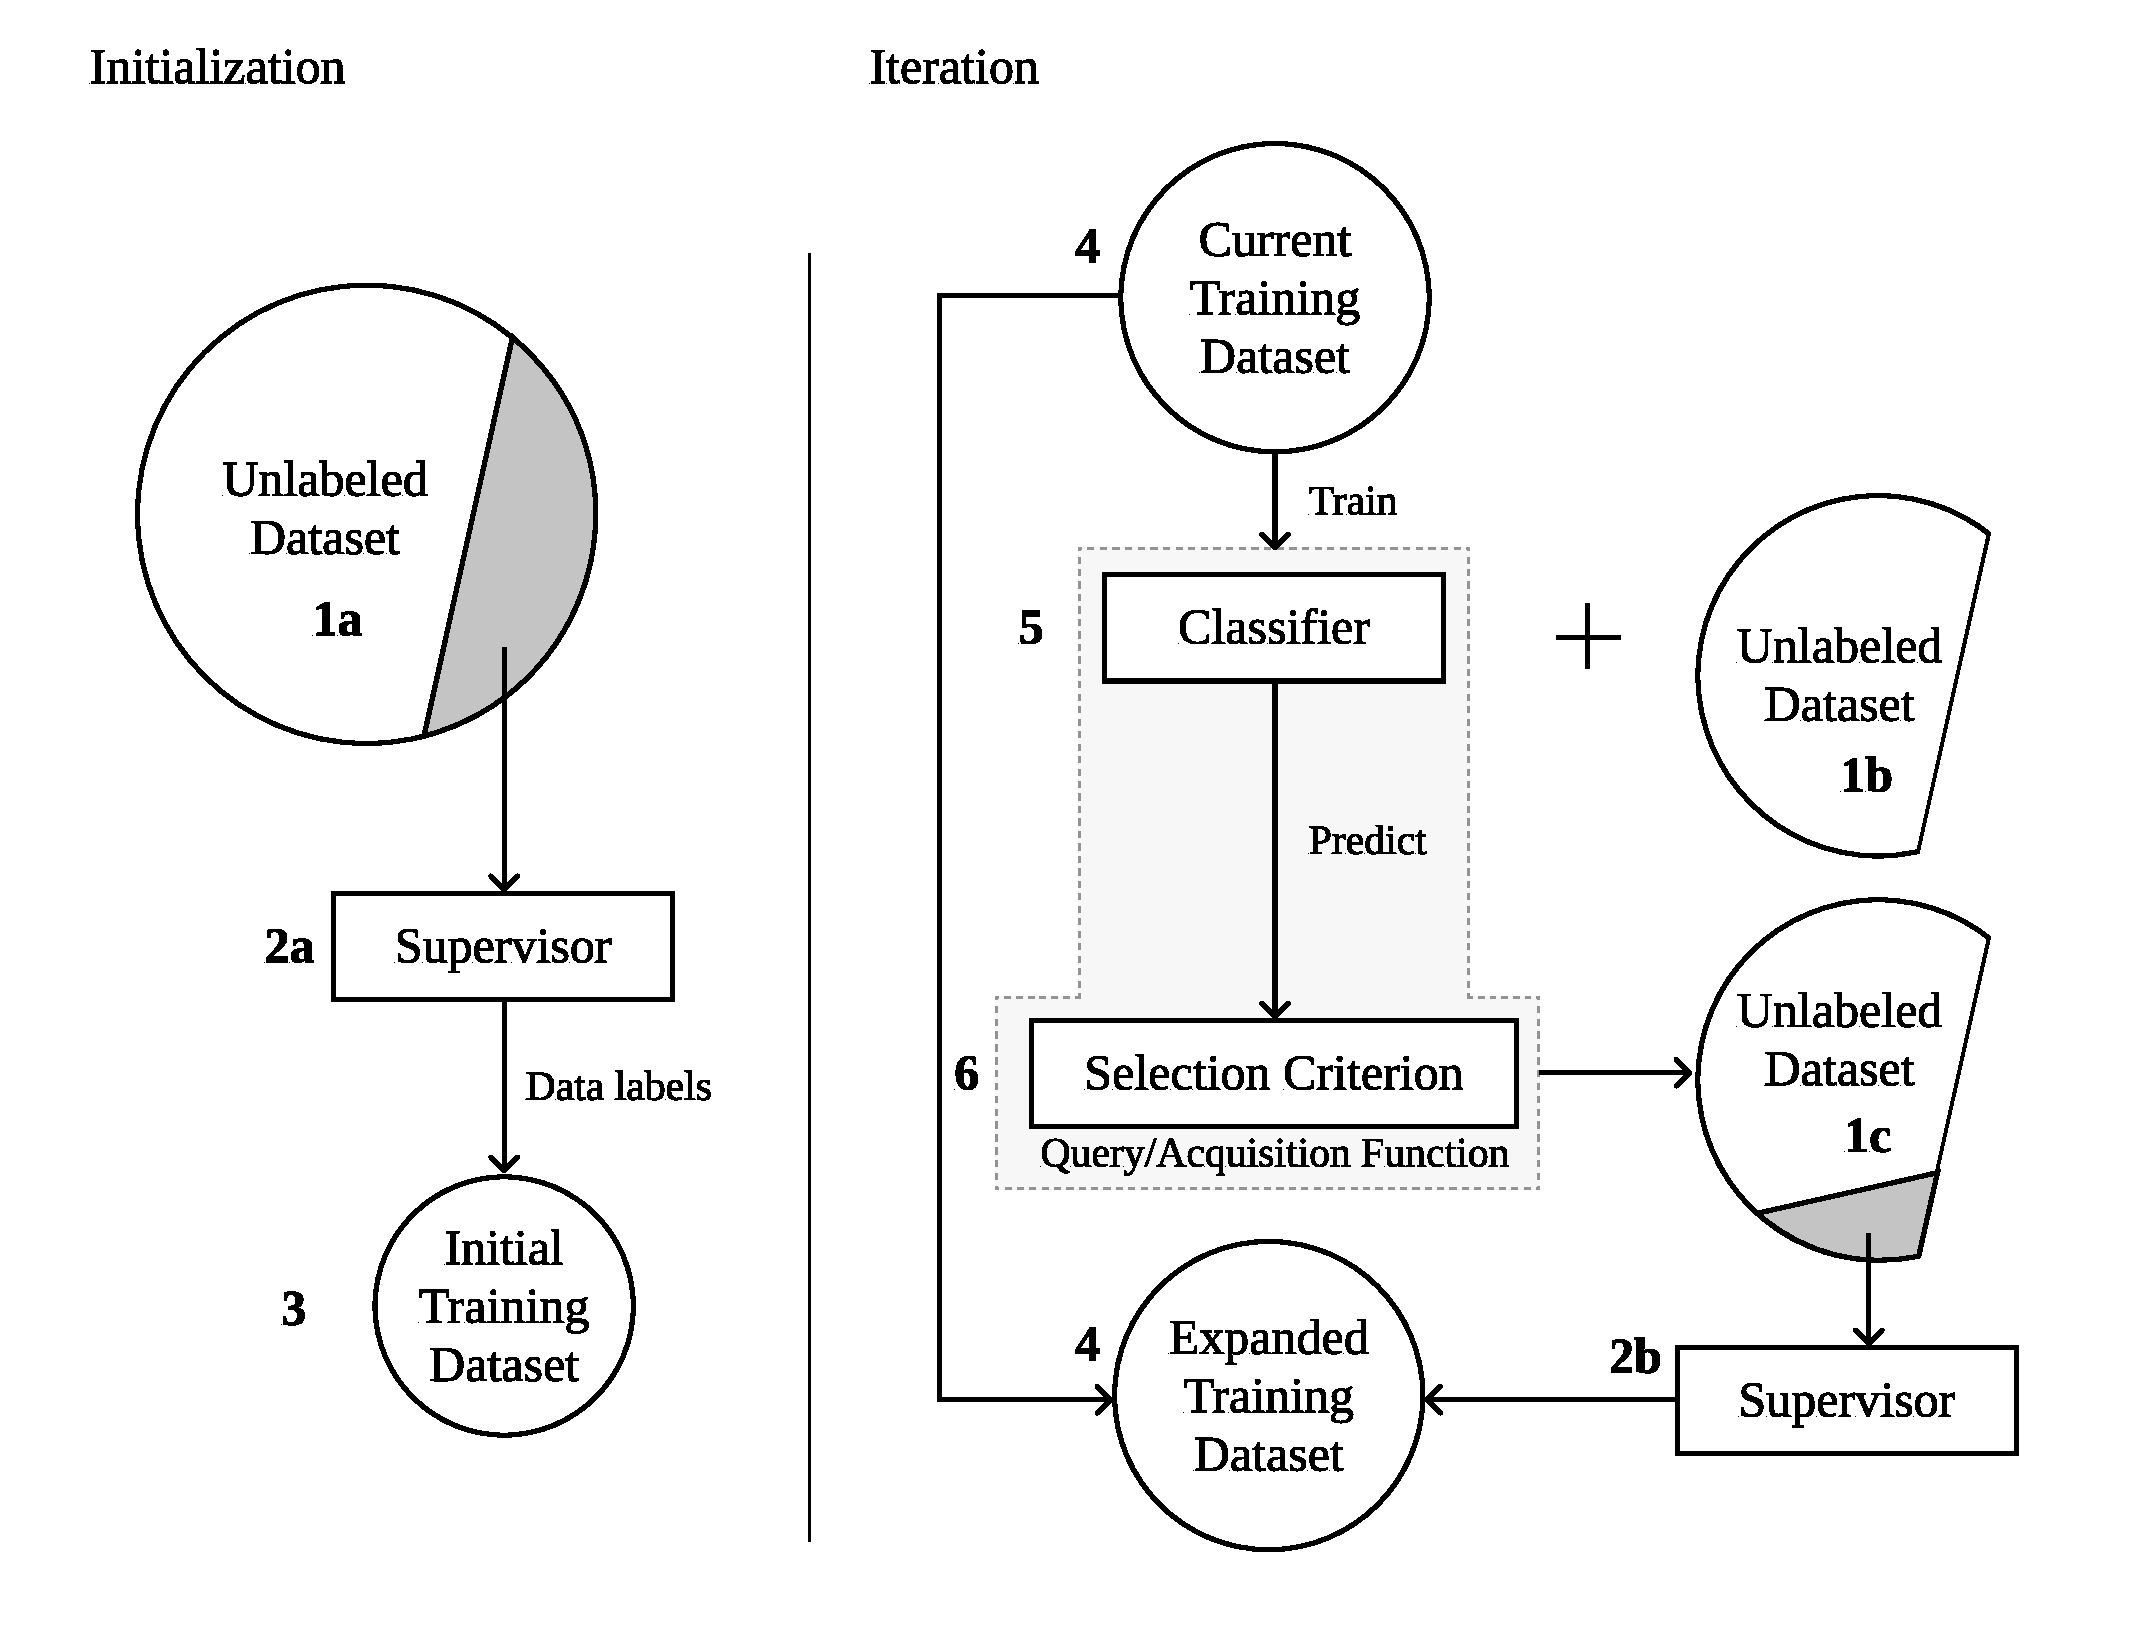
\includegraphics[width=.7\linewidth]{al_typical}
	\caption{Diagram depicting the typical AL framework.
    }~\label{fig:al_typical}
\end{figure}

A common challenge found in AL tasks is ensuring the consistency of AL over
different initializations~\cite{Kottke2017}. There are two factors involved in
this phenomenon. On one hand, the implementation of the same method over
different initializations may result in significantly different initial
training samples, amounts to varying accuracy curves. On the other hand, the
lack of a robust selection criterion and/or classifier may
also result in inconsistencies across AL experiments with different
initializations. This phenomenon was observed and documented in a LULC
classification context in~\cite{tuia2011using}.

The classification method plays a central role in the efficacy of AL. The
classifier used should be able to generalise with a relatively small training
dataset. Specifically, deep learning models are used in image classification
due to its capability of producing high quality predictions. Although, to make
such models generalizable the training set must be large enough, making its
suitability for AL applications an open challenge~\cite{Cao2020, Wu2020,
Bi2019}. Some studies in the Remote Sensing domain were developed to address
this gap. In~\cite{Cao2020, Bi2019}, the authors propose a deep learning-based
AL approach by training the same Convolutional Neural Network incrementally
across iterations and smoothen the decision boundaries of the model using the
Markov Random Field model and a Best-versus-Second Best labelling approach.
This allows the introduction of additional data variability in the final
training dataset. Another study~\cite{Wu2020} combined transfer learning,
active classification and segmentation techniques for vehicle detection. By
combining different techniques, they were able to produce a classification
mechanism that performed well when the amount of training data is limited.
However, the exploration of advanced deep learning classifiers in AL is
still limited. In~\cite{Hu2020}, the authors show that deep learning
classifiers performs well on LULC classification, but are still not
generalizable for different geographical regions or periods. Specifically, AL
methods are still incapable of providing generalizable deep learning
classifiers, which benefit from multiple advantages. The development of
Convolutional Neural Networks with both 2 and 3-dimensional convolutions was
explored in~\cite{Roy2019} and reported superior classification performance on
benchmark datasets. However, a large amount of training data was used to
produce the final classification map.

Selecting an efficient selection criterion is particularly important to find
the instances closest to the decision border (\textit{i.e.}, instances
difficult to classify)~\cite{Shrivastava2021}. Therefore, many AL related
studies focus on the design of the query/acquisition function~\cite{Su2020}.

\subsection{Non-informed selection criteria}

Only one non-informed (\textit{i.e.}, random) selection criterion was found in
the literature. Random sampling selects unlabeled instances without
considering any external information produced by the chooser. Since the method
for selecting the unlabeled instances is random, this method disregards the
usage of a chooser and is comparatively worse than any other selection
criterion. However, random sampling is still a powerful baseline
method~\cite{Cawley2011}. 

\subsection{Ensemble-based selection criteria}

Ensemble disagreement is based on the class predictions of a set of
classifiers. The disagreement between all the predictions for a given
instance is a common measure for uncertainty, although computationally
inefficient~\cite{Ruzicka2020,Pasolli2016}. It is calculated using the set of
classifications over a single instance, given by the number of votes
assigned to the most frequent class~\cite{Shrivastava2021}. This method was
implemented successfully for complex applications such as deep active
learning~\cite{Ruzicka2020}.

Multiview~\cite{Muslea2006} consists on the training of multiple independent
classifiers using different views, which correspond to the selection of subsets
of features or instances in the dataset. Therefore, it can be seen as a
bootstrap aggregation (bagging) ensemble disagreement method. It is represented
by the maximum disagreement score out of set of disagreements calculated for
each view~\cite{Shrivastava2021}. A lower value for this metric means a higher
classification uncertainty. Multiview-based maximum disagreement has been
successfully applied to hyper-spectral image classification in~\cite{Di2012}
and~\cite{Zhou2014}.

An adapted disagreement criterion for an ensemble of $k$-nearest neighbors has
been proposed in~\cite{Pasolli2016}. This method employs a $k$-nearest
neighbors classifier and computes an instance's classification uncertainty
based on the neighbors' class frequency using the maximum disagreement metric
over varying values for $k$. As a result, this method is comparable to
computing the dominant class' score over a weighted $k$-nearest neighbors
classifier. This method was also used on a multimetric active learning
framework~\cite{Zhang2016}.

Another relevant ensemble-based selection criterion is the binary random
forest-based query model~\cite{Su2020}. This method employs a one-versus-one
ensemble method to demonstrate an efficient data selection method using the
estimated probability of each binary random forest and determining the
classification uncertainty based on the probabilities closest to 0.5
(\textit{i.e.}, the least separable pair of classes are used to determine the
uncertainty value). However, this study fails to compare the proposed method
with other benchmark methods, such as random sampling.

\subsection{Entropy-based criteria}

A number of contributions have focused on entropy-based querying. The
application of entropy is common among active deep learning
applications~\cite{Aghdam2019}, where the training of an ensemble of
classifiers is often too expensive. 

Entropy query-by-bagging (EQB), also defined as maximum
entropy~\cite{Liu2020}, is an ensemble approach of the entropy selection
criterion, originally proposed in~\cite{Tuia2009}. This strategy uses the set
of predictions produced by the ensemble classifier to calculate those many
entropy measurements. The estimated uncertainty measure for one instance is
given by the maximum entropy within that set. EQB was observed to be an
efficient selection criterion. Specifically,~\cite{Shrivastava2021} applied
EQB on hyper-spectral remote sensing imagery using Support Vector Machines
(SVM) and Extreme Learning Machines (ELM) as choosers, achieving optimal
results when combining EQB with ELM\@. Another study successfully implemented
this method on an active deep learning application~\cite{Liu2020}. Another
study improved over this method with a normalized EQB selection
criterion~\cite{Copa2010}.

\subsection{Other relevant criteria}

Margin Sampling is a SVM-specific criterion, based on the distance of a given
point to the SVM's decision boundary~\cite{Shrivastava2021}. This method is
less popular than the remaining methods because it is limited to one type of
chooser (SVMs). One extension of this method is the multiclass level
uncertainty~\cite{Shrivastava2021}, calculated by subtracting the instance's
distance to the decision boundaries of the two most probable
classes~\cite{Demir2011}.

The Mutual Information-based (MI) criterion selects the new training instances
by maximizing the mutual information between the classifier and class labels
in order to select instances from regions that are difficult to classify.
Although this method is commonly used, it is frequently outperformed by the
breaking ties selection criterion~\cite{Li2011,Liu2018}.

The breaking ties (BT) selection criterion was originally introduced
in~\cite{Luo2003}. It consists of the subtraction between the probabilities of
the two most likely classes. Another related method is Modified Breaking Ties
scheme (MBT), which aims at finding the instances containing the largest
probabilities for the dominant class~\cite{Liu2018,Li2012a}

Another type of selection criteria identified is the loss prediction
method~\cite{Yoo2019}. This method replaces the selection criterion with a
predictor whose goal is to estimate the chooser's loss for a given
prediction. This allows the new classifier to estimate the prediction loss on
unlabeled instances and select the ones with the highest predicted loss.

Some of the literature fails to specify the strategy employed, although
inferring it is generally intuitive. For example,~\cite{Ertekin2007}
successfully used AL to address the imbalanced learning problem. They employed
an ensemble of SVMs as the chooser, as well as an ensemble-based selection
criterion. All of the research found related to this topic focused on the
improvement of AL through modifications on the selection criterion and
classifiers used. None of these publications proposed significant variations
to the original AL framework.

\section{Artificial Data Generation Approaches}~\label{sec:ovs-sota-al-generator}

The generation of artificial data is a common approach to address imbalanced
learning tasks~\cite{Kaur2019}, as well as improving the effectiveness of
supervised learning tasks~\cite{DeVries2017}. In recent years some
sophisticated data generation approaches were developed. However, the scope of
this work is to propose the integration of a generator within the AL
framework. To do this, we will focus on heuristic data generation approaches,
specifically, oversamplers.

Heuristic data resampling methods employ local and/or global information to
generate new, relevant, non-duplicate instances. These methods are most
commonly used to populate minority classes and balance the between-class
distribution of a dataset. The Synthetic Minority Oversampling Technique
(SMOTE)~\cite{Chawla2002} is a popular heuristic oversampling algorithm,
proposed in 2002. The simplicity and effectiveness of this method contributes
to its prevailing popularity. It generates a new instance through a linear
interpolation of a randomly selected minority-class instance and one of its
randomly selected $k$-nearest neighbors. The implementation of SMOTE for LULC
classification tasks has been found to improve the quality of the predictors
used~\cite{Jozdani2019,Bogner2018}. Despite its popularity, its drawbacks
motivated the development of other oversampling methods~\cite{Douzas2019}.

Geometric SMOTE (G-SMOTE)~\cite{Douzas2019} introduces a modification of the
SMOTE algorithm in the data generation mechanism to produce artificial
instances with higher variability. Instead of generating artificial data as a
linear combination of the parent instances, it is done within a deformed,
truncated hyper-spheroid. G-SMOTE generates an artificial instance
$\overrightarrow{z}$ within a hyper-spheroid, formed by selecting a minority
instance $\overrightarrow{x}$ and one of its nearest neighbors
$\overrightarrow{y}$, as shown in Figure~\ref{fig:data_generation}. The
truncation and deformation parameters define the shape of the spheroid's
geometry. The method also modifies the selection strategy for the $k$-nearest
neighbors, accepting the generation of artificial instances using instances
from different classes, as shown in Figure~\ref{fig:data_generation}d. The
modification of both selection and generation mechanisms addresses the main
drawbacks found in SMOTE, the generation of both noisy data (\textit{i.e.,}
generate minority class instances within majority class regions) and
near-duplicate minority class instances~\cite{Douzas2019}. G-SMOTE has shown
superior performance when compared with other oversampling methods for LULC
classification tasks, regardless of the classifier sed~\cite{Douzas2019rs}.

\begin{figure}
	\centering
	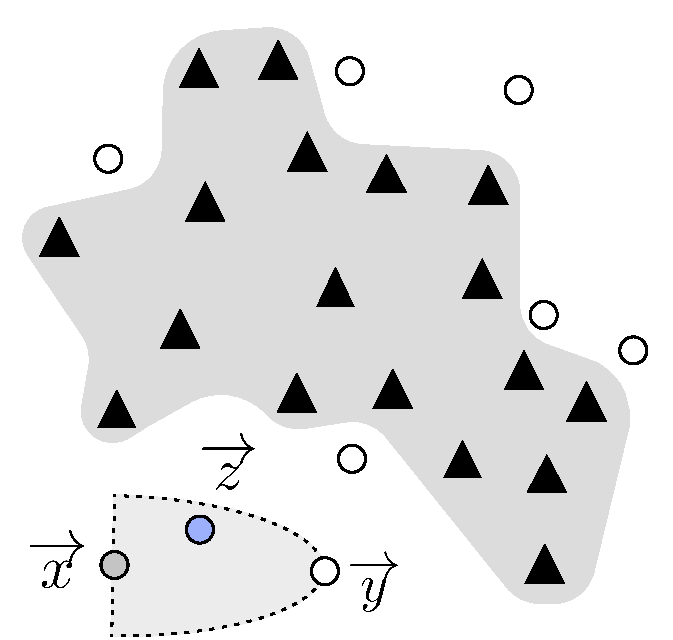
\includegraphics[width=.35\linewidth]{data_generation}
    \caption[Example of G-SMOTE's generation process.]{Example of G-SMOTE's
        generation process. G-SMOTE randomly selects instance
        $\protect\overrightarrow{x}$ and one of its nearest neighbors
        $\protect\overrightarrow{y}$ to produce instance
        $\protect\overrightarrow{z}$.
    }~\label{fig:data_generation}
\end{figure}

\section{Proposed method}~\label{sec:proposed-method-al-generator}

Within the literature identified, most of the work developed in the AL domain
revolved around improving the quality of classification algorithms and/or
selection criteria. Although these methods allow earlier convergence of the
AL iterative process, the impact of these methods are only observed between
iterations. Consequently, none of these contributions focused on the
definition of decision borders within iterations. The method proposed in this
paper modifies the AL framework by introducing an artificial data generation
step within AL's iterative process. We define this component as the generator
and is intended to be integrated into the AL framework as shown in
Figure~\ref{fig:al_new}. 

This modification, by using a new source of data to augment the training set,
leverages the data annotation work conducted by the human operator. The
artificial data that is generated between iterations reduces the amount of
labeled data required to reach optimal performance and lower the amount of
human labor required to train a classifier to its optimal performance. This
process lowers the annotation and overall training costs by translating some
of the annotation cost into computational cost.

\begin{figure}
	\centering
	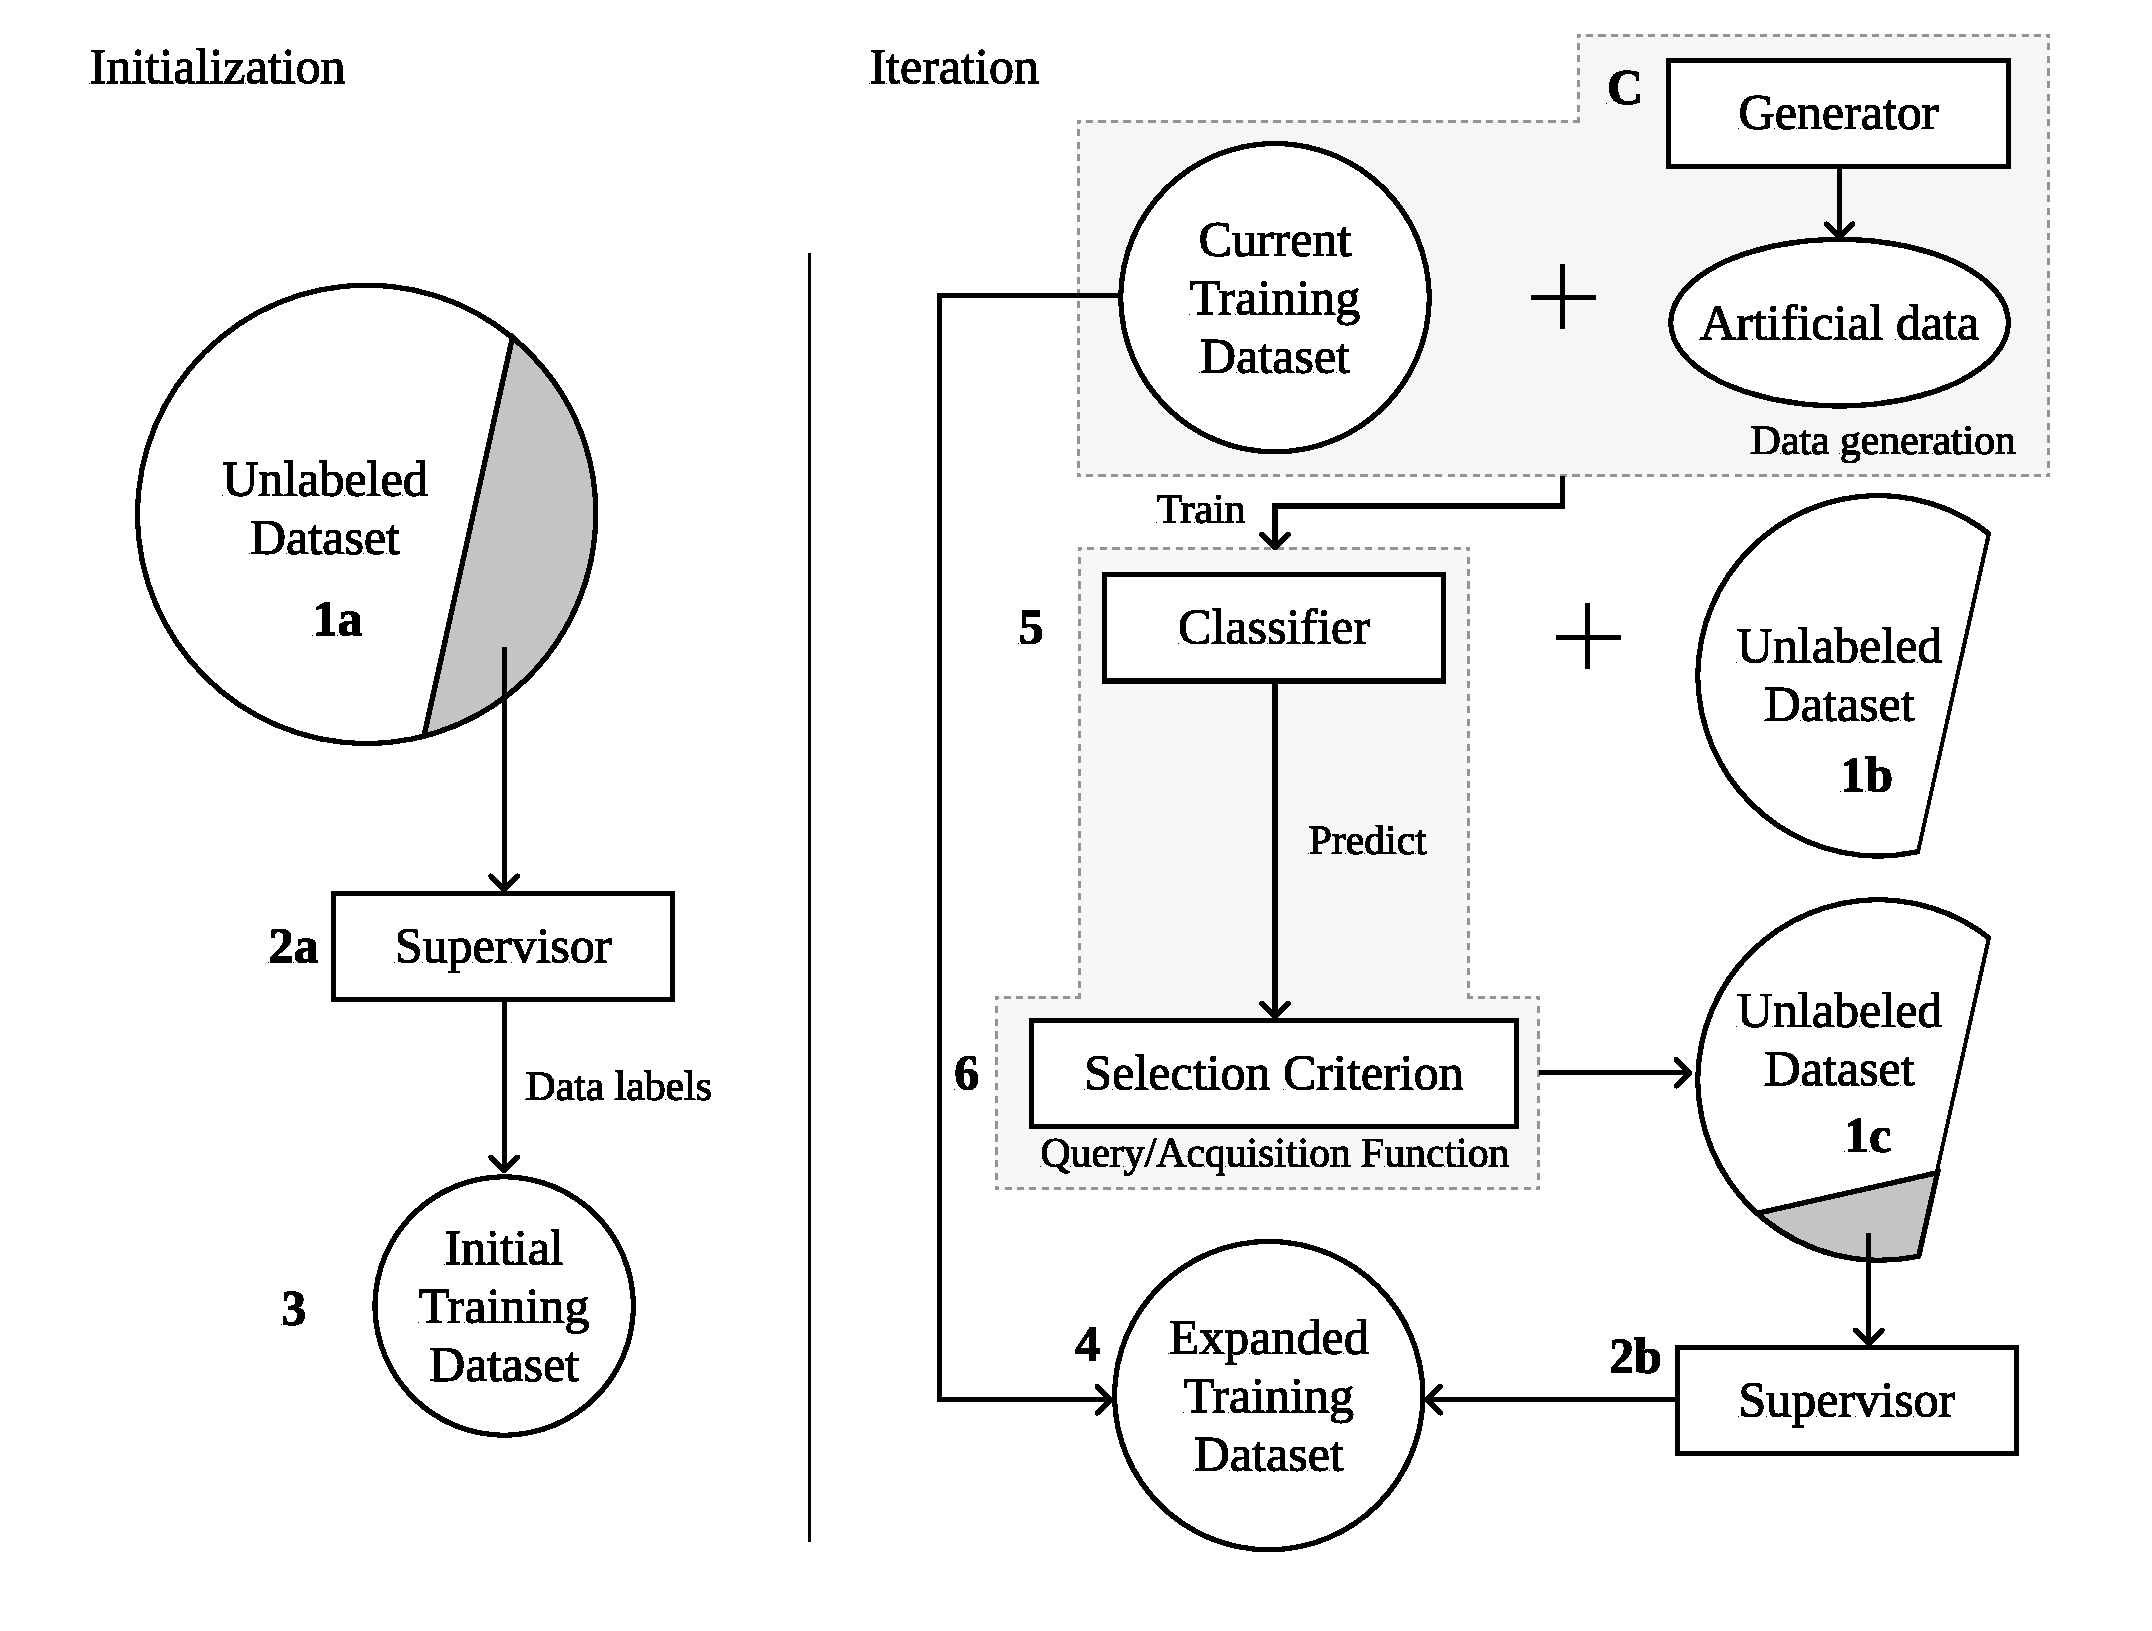
\includegraphics[width=.7\linewidth]{al_new}
    \caption[Proposed AL framework.]{%
        Proposed AL framework. This paper's contribution comprises a change in
        the AL framework through the introduction of a data generation
        mechanism, represented as the generator (marked with~\textit{C}),
        which is used to add artificial instances to the training dataset.
    }~\label{fig:al_new}
\end{figure}

This method leverages the capability of artificial data to introduce more data
variability into the augmented dataset and facilitate the chooser's training
phase with a more consistent definition of the decision boundaries at each
iteration. Therefore, any algorithm capable of producing artificial data, be
it agnostic or specific to the domain, can be employed. The artificial data is
only used to train the classifiers involved in the process and is discarded
once the training phase is completed. The remaining steps in the AL framework
remain unchanged. This method addresses the limitations found in the previous
sections:

\begin{enumerate}
    \item The convergence of classification performance should be anticipated
        with the clearer definition of the decision boundaries across
        iterations.
    \item Annotation cost is expected to reduce as the need for labeled
        instances reduces along with the early convergence of the
        classification performance.
    \item The class imbalance bias observed in typical classification tasks, as
        well as in AL is mitigated by balancing the class frequencies at each
        iteration.
\end{enumerate}

Although the performance of this method is shown within a LULC classification
context, the proposed framework is independent from the domain. The high
dimensionality of remotely sensed imagery make its classification particularly
challenging when the availability of labeled data is scarce and/or comes at a
high cost, being subjected to the curse of dimensionality. Consequently, it is
a relevant and appropriate domain to test this method.


\section{Methodology}~\label{sec:methodology-al-generator}

In this section we describe the datasets, evaluation metrics, oversampler,
classifiers, software used and the procedure developed. We demonstrate the
proposed method's efficiency over 7 datasets, sampled from publicly available,
well-known remote sensing hyperspectral scenes frequently found in remote
sensing literature. The datasets and sampling strategy are described in
Subsection~\ref{sec:datasets-al-generator}. On each of these datasets, we apply 3 different
classifiers over the entire training set to estimate the optimal
classification performance, the original AL framework as the baseline
reference and the proposed method using G-SMOTE as a generator, described in
Subsection~\ref{sec:machine_learning_algorithms-al-generator}. The metrics used to estimate
the performance of these algorithms are described in
Subsection~\ref{sec:evaluation_metrics-al-generator}. Finally, the experimental procedure
is described in Subsection~\ref{sec:experimental_procedure-al-generator}. 

Our methodology focuses on two objectives: (1) Comparison of optimal
classification performance among active learners and traditional supervised
learning and (2) Comparison of classification convergence efficiency among AL
frameworks.

\subsection{Datasets}~\label{sec:datasets-al-generator}

The datasets used were extracted from publicly available repositories
containing hyperspectral images and ground truth data. Additionally, all
datasets were collected using the same sampling procedure. The description of
the hyperspectral scenes used in this study is provided in
Table~\ref{tab:rs_scene_description}. These scenes were chosen because of
their popularity in the research community and their high baseline
classification scores. Consequently, demonstrating an outperforming method in
this context is particularly challenging and valuable.

\begin{table}
	\centering
    \addtolength{\leftskip} {-2cm}
    \addtolength{\rightskip}{-2cm}
    \pgfplotstabletypeset[
        col sep=semicolon,
        string type,
        every head row/.style={%
            before row=\toprule,
            after row=\midrule
        },
        every last row/.style={after row=\bottomrule},
        string type,
    ]{figures/al-generator-lulc/rs_scene_description.csv}
    \caption[Description of the hyperspectral scenes used in this experiment.]{%
        Description of the hyperspectral scenes used in this experiment. The
        column ``Res. (m)'' refers to the resolution of the sensors (in
        meters) that captured each of the scenes.
    }~\label{tab:rs_scene_description}
\end{table}

The Indian Pines scene~\cite{Baumgardner2015} is composed of agriculture fields
in approximately two thirds of its coverage, low density buildup areas and
natural perennial vegetation in the remainder of its area (see
Figure~\ref{fig:scenes}a). The Pavia Centre and University scenes are
hyperspectral, high-resolution images containing ground truth data composed of
urban-related coverage (see Figures~\ref{fig:scenes}b
and~\ref{fig:scenes}c). The Salinas and Salinas A scenes contain
at-sensor radiance data. As subset of Salinas, the Salinas A scene contains
contains the vegetables fields present in Salinas and the latter is also
composed of bare soils and vineyard fields (see Figures~\ref{fig:scenes}d
and~\ref{fig:scenes}e). The Botswana scene contains ground truth data
composed of seasonal swamps, occasional swamps, and drier woodlands located in
the distal portion of the Delta (see Figure~\ref{fig:scenes}f). The Kennedy
Space Center scene contains a ground truth composed of both vegetation and
urban-related coverage (see Figure~\ref{fig:scenes}g).

\begin{figure}
	\centering
	\includegraphics[width=.85\linewidth]{scenes}
    \caption[Gray scale visualization of a band and ground truth of each scene
        used in this study.]{%
        Gray scale visualization of a band (top row) and ground truth (bottom
        row) of each scene used in this study. (a) Indian Pines, (b) Pavia
        Centre, (c) Pavia University, (d) Salinas, (e) Salinas A, (f)
        Botswana, (g) Kennedy Space Center 
    }~\label{fig:scenes}
\end{figure}

The sampling strategy is similar to all datasets. The pixels without a ground
truth label are first discarded. All the classes with cardinality lower than
150 are also discarded. This is done to maintain feasible Imbalance Ratios (IR)
across datasets (where $IR = \frac{count(C_{maj})}{count(C_{min})}$). Finally,
a stratified sample of 1500 instances are selected for the experiment. The
resulting datasets are described in
Table~\ref{tab:datasets_description_al_generator}. The
motivation for this strategy is three fold: (1) reduce the datasets to a
manageable size and allow the experimental procedure to be completed within a
feasible time frame, (2) ensure the relative class frequencies in the scenes
are preserved and (3) ensure equivalent analyses across datasets and AL
frameworks. In this context, a fixed number of instances per dataset is
especially important to standardize the AL-related performance metrics.

\begin{table}
    \centering
    \addtolength{\leftskip} {-2cm}
    \addtolength{\rightskip}{-2cm}
    \pgfplotstabletypeset[
        col sep=comma,
        string type,
        every head row/.style={%
            before row=\toprule,
            after row=\midrule
        },
        every last row/.style={after row=\bottomrule},
    ]{figures/al-generator-lulc/datasets_description.csv}
    \caption[Description of the datasets collected from each corresponding
        scene.]{%
        Description of the datasets collected from each corresponding scene.
        The sampling strategy is similar to all scenes.
    }~\label{tab:datasets_description_al_generator}
\end{table}

\subsection{Machine Learning Algorithms}~\label{sec:machine_learning_algorithms-al-generator}

We use two different types of ML algorithms. A data generation algorithm, used
to form the generator, and classification algorithms, used to calculate the
classification uncertainties in the unlabeled dataset and predict the class
labels in the validation and test sets.

Although any method capable of generating artificial data can be used as a
generator, the one used in this experiment is an oversampler, originally
developed to deal with imbalanced learning problems. Specifically, we chose
G-SMOTE, a state-of-the-art oversampler.

Three classification algorithms are used. We use different types of
classifiers to test the framework's performance under varying situations:
neighbors-based, linear and ensemble models. The neighbors-based classifier
chosen was $K$-nearest neighbors (KNN)~\cite{Cover1967}, a logistic regression
(LR)~\cite{Nelder1972} is used as the linear model and a random forest
classifier (RFC)~\cite{Ho1995} was used as the ensemble model.

The acquisition function is completed by testing three different selection
criteria. Random selection is used as a baseline selection criterion, whereas
entropy and breaking ties are used due to their popularity and independence of
the classifier used.

\subsection{Evaluation Metrics}~\label{sec:evaluation_metrics-al-generator}

Since the datasets used in this experiment have an imbalanced distribution of
class frequencies, metrics such as the \textit{Overall Accuracy} (OA) and
\textit{Kappa coefficient} are insufficient to accurately depict
classification performance~\cite{Olofsson2013, Pontius2011}. Instead, metrics
such as Producer's Accuracy (or \textit{Recall}) and User's Accuracy (or
\textit{Precision}) can be used. Since they consist of ratios based on
True/False Positives (TP and FP) and Negatives (TN and FN), they provide per
class information regarding the classifier's classification performance.
However, in this experiment, the meaning and number of classes available in
each dataset varies, making these metrics difficult to synthesize.

The performance metric \textit{Geometric mean} (G-mean) and
\textit{F-score} are less sensitive to the data imbalance
bias~\cite{Jeni2013, Kubat1997}.  Therefore, we employ both of these
scorers. G-mean consists of the geometric mean of $Specificity = \frac{TN}{TN
+ FP}$ and $Sensitivity = \frac{TP}{TP+FN}$ (also known as
\textit{Recall})~\cite{Kubat1997}. Both metrics are calculated in a multiclass
context considering a one-versus-all approach. For multiclass problems, the
\textit{G-mean} scorer is calculated as its average per class values: 
        
\begin{equation*}
    \textit{G-mean} = \sqrt{\overline{Sensitivity}_i \times
    \overline{Specificity}_i}
\end{equation*}

The F-score performance metric is the harmonic mean of \textit{Precision} and
\textit{Recall}. The two metrics are also calculated considering a
one-versus-all approach. The \textit{F-score} for the multi-class case can be
calculated using its average per class values~\cite{He2009}:

\begin{equation*}
    \textit{F-score}=2\frac{\overline{Precision} \times
    \overline{Recall}}{\overline{Precision} + \overline{Recall}}
\end{equation*}
 
The comparison of classification convergence across AL frameworks and
selection criteria is done using 2 AL-specific performance metrics.
Particularly, we follow the recommendations found in~\cite{Kottke2017}. Each
AL configuration is evaluated using the \textit{Area Under the Learning Curve}
(AULC) performance metric. It is the sum of the classification performance
values of all iterations. To facilitate the analysis of the results, we fix
the range of this metric between $[0,1]$ by dividing it with the total amount
of iterations (\textit{i.e.}, the maximum performance area). 

The \textit{Data Utilization Rate} (DUR)~\cite{Reitmaier2013} metric consists
of the ratio between the number of instances required to reach a given G-mean
score threshold by an AL strategy and an equivalent baseline strategy. For
easier interpretability, we simplify this metric by using the percentage
of training data used by an AL strategy to reach the performance threshold,
instead of presenting these values as a ratio of the baseline strategy. The
DUR metric is measured at 9 different performance levels, between
0.6 and 0.95 G-mean scores at a 0.05 step.

\subsection{Experimental Procedure}~\label{sec:experimental_procedure-al-generator}

A common practice in methodological evaluations is the implementation of an
offline experiment~\cite{Kagy2019}. It consists of using an existing set of
labeled data as a proxy for the population of unlabeled instances. Because the
dataset is already fully labeled, the supervisor's typical annotation process
involved in each iteration is done at zero cost. Each AL and classifier
configuration is tested using a stratified 5-fold cross validation testing
scheme. For each round, the larger partition is split in a stratified fashion
to form a training and validation set (containing 20\% of the original
partition). The validation set is used to evaluate the convergence efficiency
of active learners; the chooser's classification performance metrics and
amount of data points used at each iteration are used to compute the AULC and
DUR\@. Additionally, within the AL iterative process, the classifier with
optimal performance on the validation set is evaluated using the test set. In
order to further reduce possible initialization biases, this procedure is
repeated 3 times with different initialization seeds and the results of all
runs are averaged (\textit{i.e.}, each configuration is trained and evaluated
15 times). Finally, the maximum performance lines are calculated using the
same approach. In those cases, the validation set is not used. The
experimental procedure is depicted in
Figure~\ref{fig:experiment_pipeline_al_generator}.

\begin{figure}
	\centering
	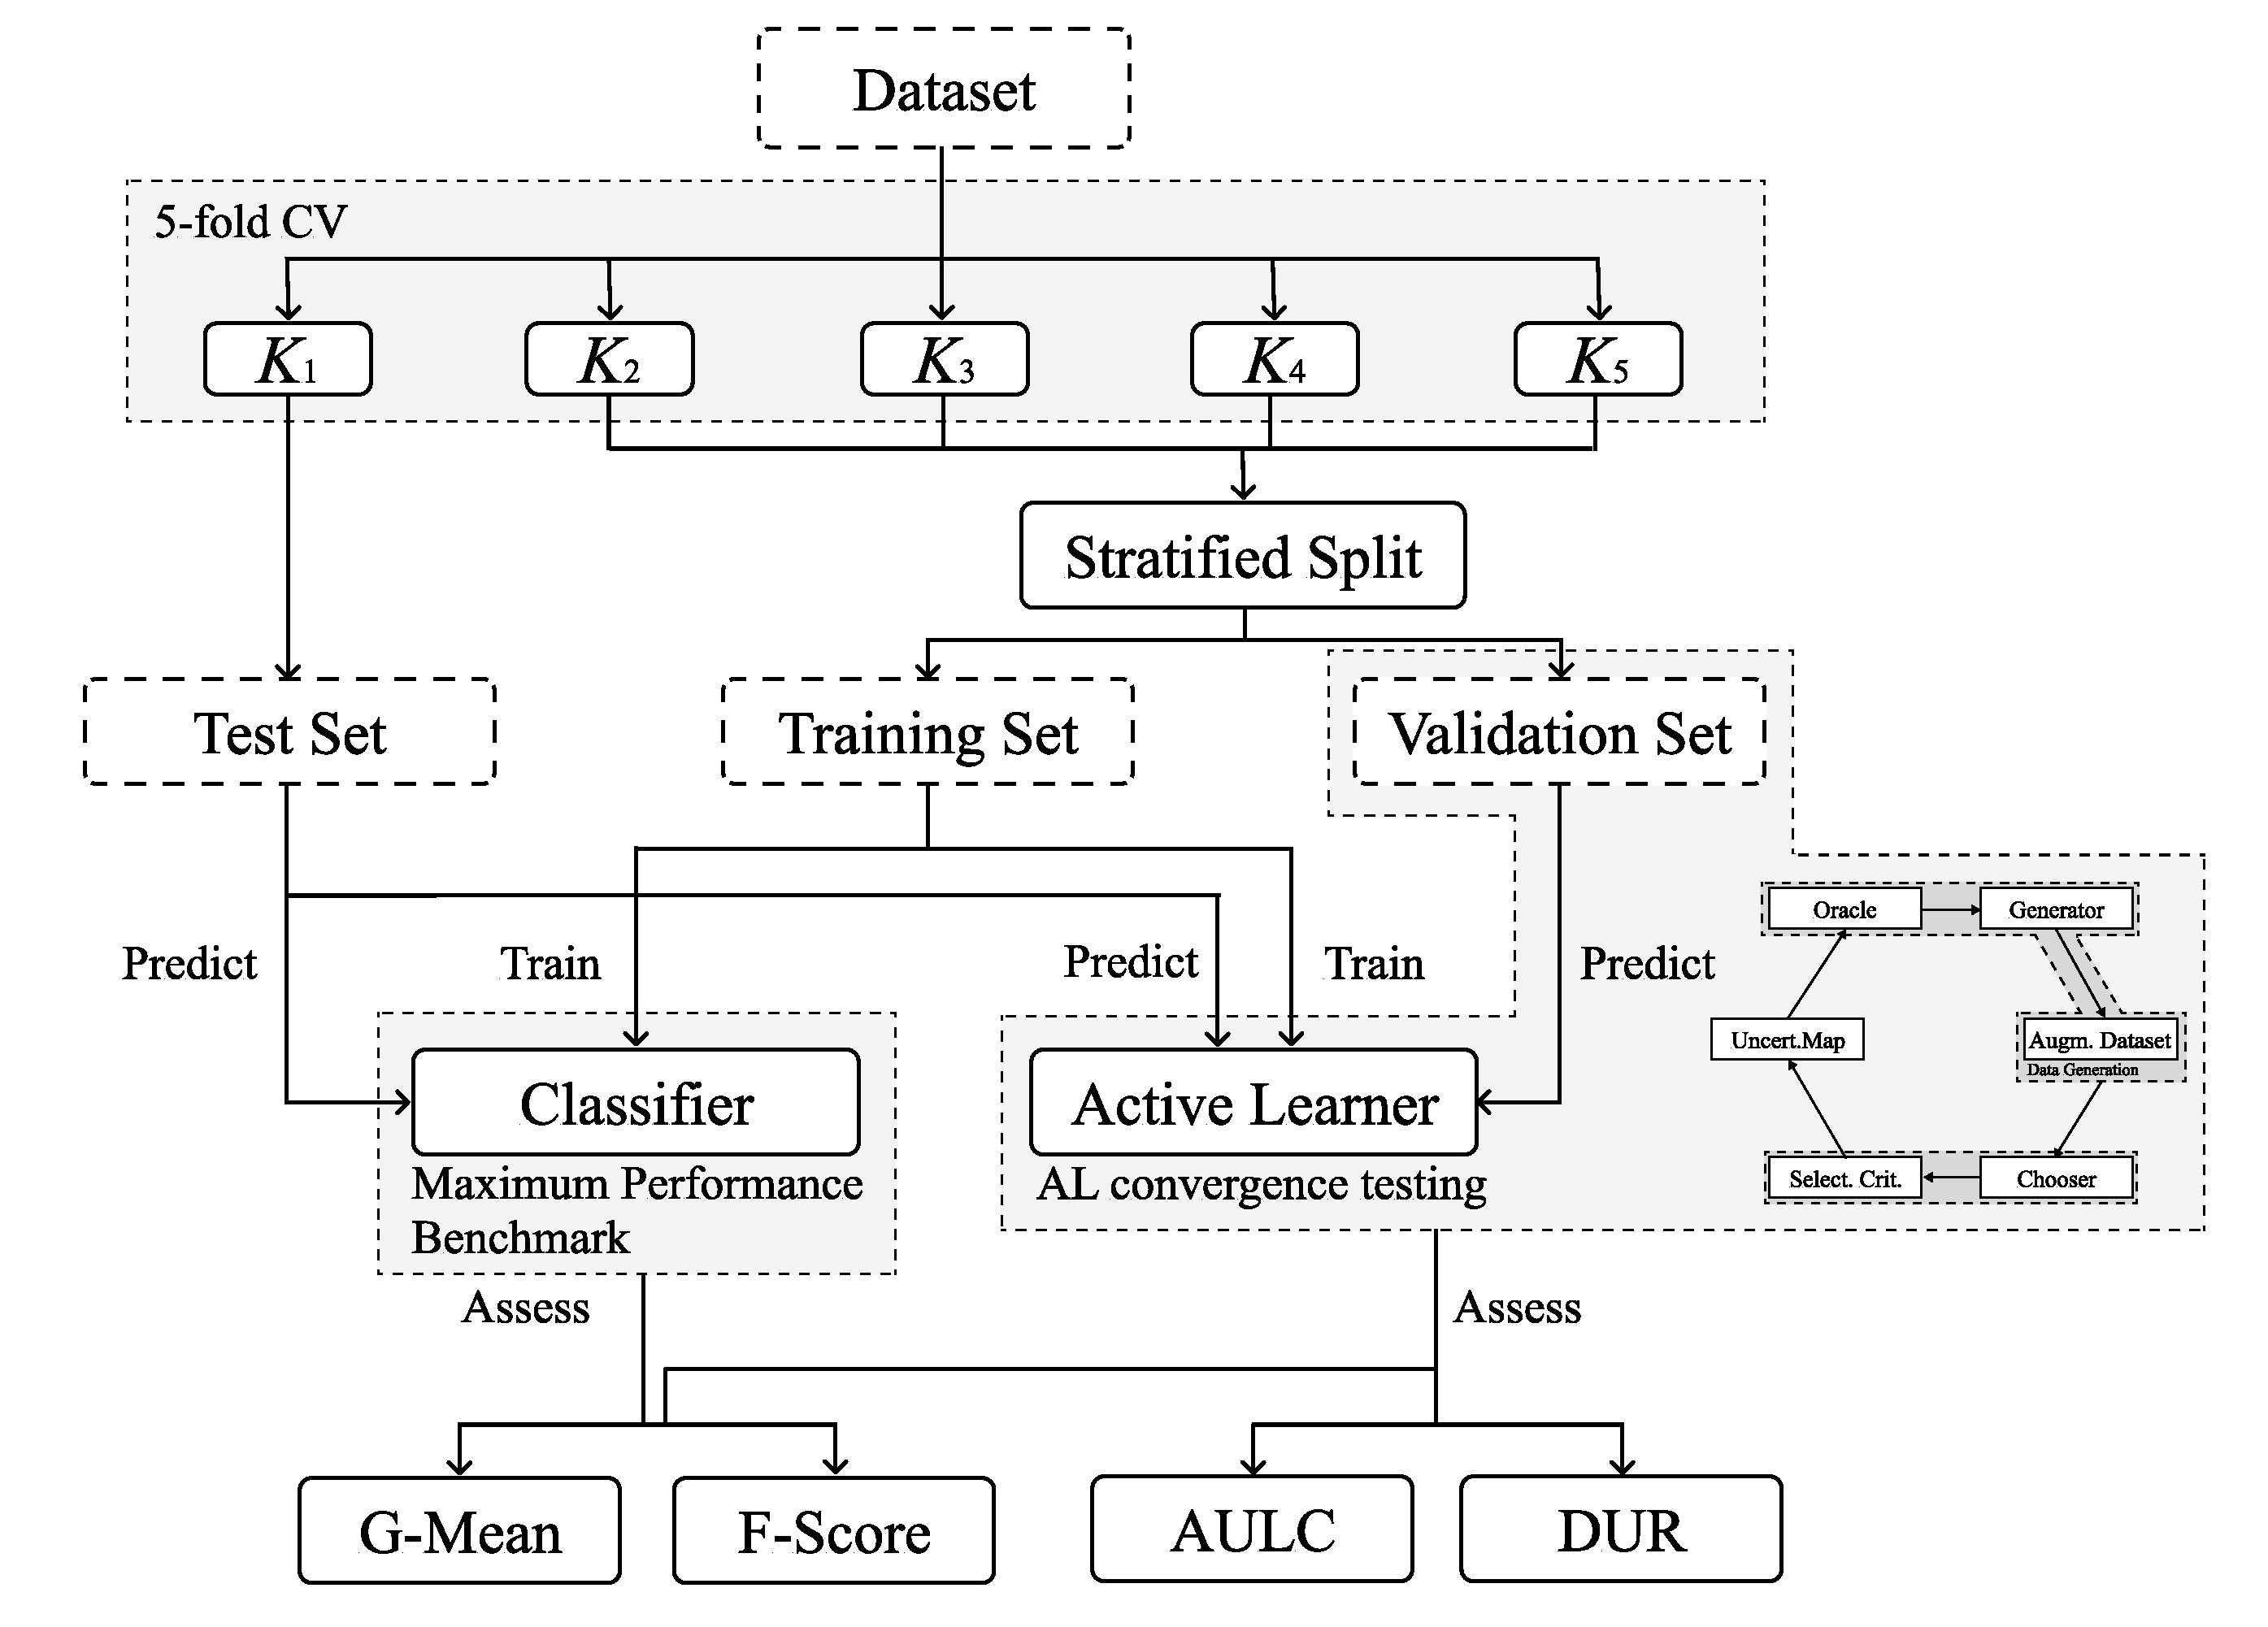
\includegraphics[width=.65\linewidth]{experiment_pipeline}
    \caption[Experimental procedure.]{%
        Experimental procedure. The datasets extracted from hyperspectral
        scenes are split in 5 folds. 1 of those (\textit{e.g.}, $K_1$) is used
        to test the optimal performance of AL algorithms and the
        classification without AL. The training set is used to iterate AL
        algorithms and train classifiers. The validation set is used to test
        the convergence of AL algorithms. The results are averaged over the 5
        folds across each of the 3 different initializations of this
        procedure.
    }~\label{fig:experiment_pipeline_al_generator}
\end{figure}

To make the AL-specific metrics comparable among active learners, the
configurations of the different frameworks must be similar. For each dataset,
the number of instances is constant to facilitate the analysis of the same
metrics. 

In most practical AL applications it is assumed that the number of instances 
in the initial training sample is too small to perform hyperparameter tuning.
Consequently, in order to ensure realistic results, our experimental procedure
does not include hyperparameter optimization. The predefined hyperparameters
are shown in Table~\ref{tab:grid_al_generator}. They were set up based on general
recommendations and default settings for the classifiers and generators used.

The AL iterative process is set up with a randomly selected initial training
sample with 15 initial samples. At each iteration, 15 additional samples are
added to the training set. This process is stopped after 49 iterations, once
50\% of the entire dataset (\textit{i.e.,} 78\% of the training set) is added
to the augmented dataset.

\begin{table}
	\centering
	\begin{tabular}{lll}
		\toprule
		Classifier & Hyperparameters      & Values             \\
		\midrule
		LR         & maximum iterations   & 10000              \\
		           & solver               & sag                \\
                   & penalty              & None               \\
		KNN        & \# neighbors         & 5                  \\
                   & weights              & uniform            \\
                   & metric               & euclidean          \\
		RF         & maximum tree depth   & None               \\
		           & \# estimators        & 100                \\
                   & criterion            & gini               \\
		\toprule
		Generator  &                      &                    \\
		\midrule
		G-SMOTE    & \# neighbors         & 5                  \\
                   & deformation factor   & 0.5                \\
                   & truncation factor    & 0.5                \\
		\bottomrule
	\end{tabular}
    \caption{Hyper-parameter definition for the classifiers and
    generator used in the experiment.}~\label{tab:grid_al_generator}
\end{table}

\subsection{Software Implementation}

The experiment was implemented using the Python programming language, along
with the Python libraries
\href{https://scikit-learn.org/stable/}{Scikit-Learn}~\cite{Pedregosa2011},
\href{https://imbalanced-learn.org/en/stable/}{Imbalanced-Learn}~\cite{JMLR:v18:16-365},
\href{https://geometric-smote.readthedocs.io/en/latest/?badge=latest}{Geometric-SMOTE},
\href{https://cluster-over-sampling.readthedocs.io/en/latest/?badge=latest}{Cluster-Over-Sampling}
and
\href{https://research-learn.readthedocs.io/en/latest/?badge=latest}{Research-Learn}
libraries. All functions, algorithms, experiments and results are provided in
the \href{https://github.com/joaopfonseca/publications/}{GitHub repository of the
project}.

\section{Results \& Discussion}~\label{sec:results-al-generator}

The evaluation of the different AL frameworks in a multiple dataset context
should not rely uniquely on the mean of the performance metrics across
datasets.~\cite{Demsar2006} recommends the use of mean ranking scores, since
the performance levels of the different frameworks varies according to the
data it is being used on. Consequently, evaluating these performance metrics
solely based on their mean values might lead to inaccurate analyses.
Accordingly, the results of this experiment are analysed using both the mean
ranking and absolute scores for each model. The rank values are assigned based
on the mean scores resulting from three different initializations of 5-fold
cross validation for each classifier and active learner. The goal of this
analysis is to understand whether the proposed framework (AL with the
integration of an artificial data generator) is capable of using less data
from the original dataset while simultaneously achieving better classification
results than the standard AL framework, \textit{i.e.}, guarantee a faster
classification convergence. 

\subsection{Results}~\label{sec:sub_results-al-generator}

Table~\ref{tab:aulc_ranks_al_generator} shows the average rankings and standard deviations
across datasets of the AULC scores for each active learner.

\begin{table}
    \centering
    \pgfplotstabletypeset[
        col sep=comma,
        string type,
        every head row/.style={%
            before row=\toprule,
            after row=\midrule
        },
        every last row/.style={after row=\bottomrule},
    ]{figures/al-generator-lulc/mean_std_aulc_ranks.csv}
    \caption[Mean rankings of the AULC metric.]{%
        Mean rankings of the AULC metric over the different datasets (7),
        folds (5) and runs (3) used in the experiment. This means that the use
        of G-SMOTE almost always improves the results of the original
        framework.
    }\label{tab:aulc_ranks_al_generator}
\end{table}

The mean AULC absolute scores are provided in Table~\ref{tab:aulc_scores_al_generator}.
These values are computed as the mean of the sum of the scores of a specific
performance metric over all iterations (for an AL configuration). In other
words, these values correspond to the average AULC over $7\ datasets \times 5\
folds \times 3\ initializations$.

\begin{table}
    \centering
    \pgfplotstabletypeset[
        col sep=comma,
        string type,
        every head row/.style={%
            before row=\toprule,
            after row=\midrule
        },
        every last row/.style={after row=\bottomrule},
    ]{figures/al-generator-lulc/mean_std_aulc_scores.csv}
    \caption[Average AULC of each AL configuration tested.]{%
        Average AULC of each AL configuration tested. Each AULC score is
        calculated using the G-mean scores of each iteration in the validation
        set. By the end of the iterative process, each AL configuration used a
        total of 750 instances of the 960 instances that compose the training
        set.
    }~\label{tab:aulc_scores_al_generator}
\end{table}

The average DURs are shown in Table~\ref{tab:optimal_data_utilization_al_generator}. They
were calculated for various G-mean scores thresholds, varying at a step of 5\%
between 60\% and 95\%. Each row shows the percentage of training data required
by the different AL configurations to reach that specific G-mean score.

\pgfplotstabletypeset[
	begin table=\begin{longtable},
	end table=\end{longtable},
	col sep=comma,
	header=true,
    columns={G-mean Score,Classifier,Standard,Proposed}, 
    string type,
    every head row/.style={before row=\toprule, after row=\midrule\endhead},
	every last row/.style={
        after row={
            \bottomrule
            \caption[Mean data utilization of AL algorithms.]{
                Mean data utilization of AL algorithms, as a percentage of the training set.
            }~\label{tab:optimal_data_utilization_al_generator}
        }
    }
]{figures/al-generator-lulc/optimal_data_utilization.csv}

The DUR of the proposed method relative to the baseline method is shown in
Figure~\ref{fig:dur_al_generator}. A DUR below 1 means that the proposed framework requires
less data to reach the same performance threshold (as a percentage, relative
to the amount of data required by the baseline framework). For instance, in the
upper left graphic we can see that the proposed framework achieves 90\%
classification using F-score while using 91\% of the amount of data used by the
traditional AL framework, in other words 9\% less data.

\begin{figure}
	\centering
	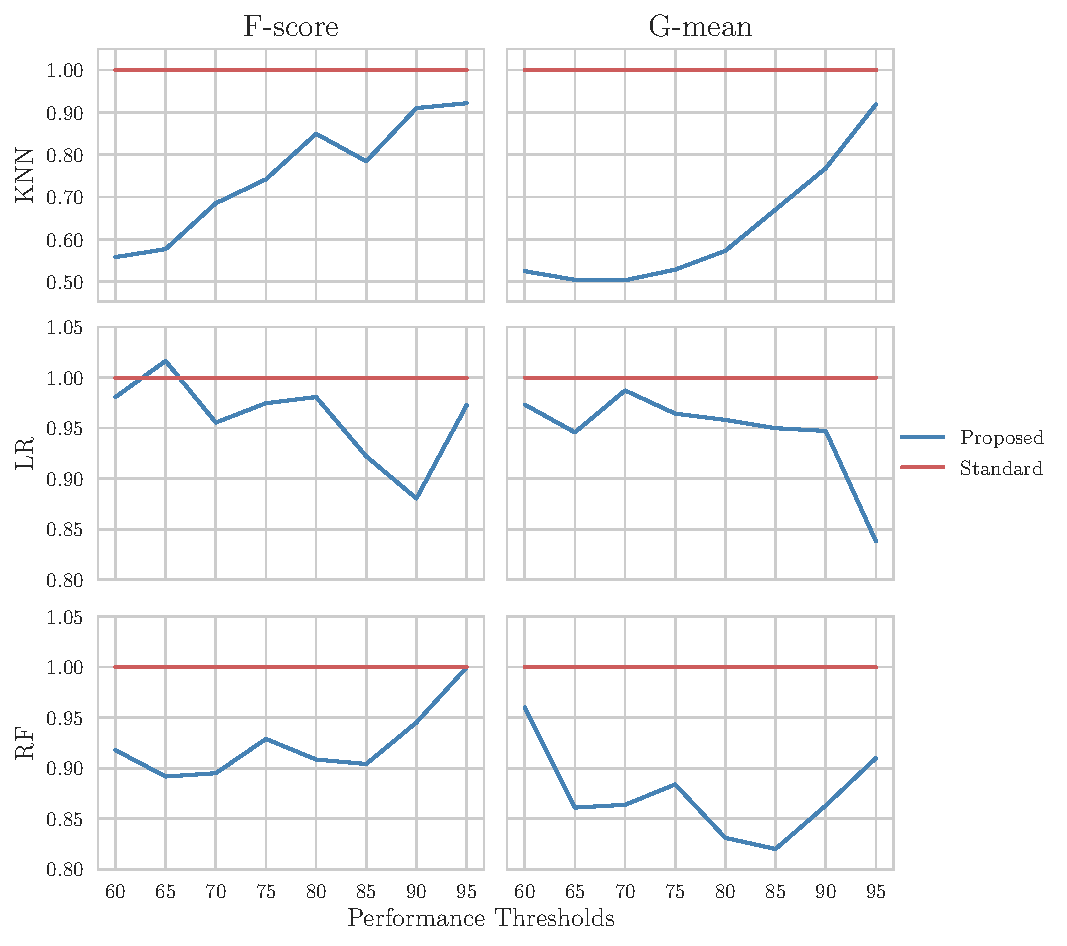
\includegraphics[width=.75\linewidth]{data_utilization_rate}
    \caption[Mean data utilization rates.]{%
        Mean data utilization rates. The y-axis shows the percentage of data
        (relative to the baseline AL framework) required to reach the
        different performance thresholds.
    }~\label{fig:dur_al_generator}
\end{figure}

The averaged optimal classification scores are shown in
Table~\ref{tab:optimal_mean_std_scores_al_generator}. The maximum performance (MP)
classification scores are shown as a benchmark and represent the performance
of the corresponding classifier using the entire training set. 

\begin{table}
    \centering
    \addtolength{\leftskip} {-2cm}
    \addtolength{\rightskip}{-2cm}
    \pgfplotstabletypeset[
        col sep=comma,
        string type,
        every head row/.style={%
            before row=\toprule,
            after row=\midrule
        },
        every last row/.style={after row=\bottomrule},
    ]{figures/al-generator-lulc/optimal_mean_std_scores.csv}
    \caption[Optimal classification scores.]{%
        Optimal classification scores. The Maximum Performance (MP)
        classification scores are calculated using classifiers trained using
        the entire training set.
    }~\label{tab:optimal_mean_std_scores_al_generator}
\end{table}

\subsection{Statistical Analysis}~\label{sec:statistical-analysis-al-generator}

The methods used to test the experiment's results must be appropriate for a
multi-dataset context. Therefore the statistical analysis is performed using
the Wilcoxon signed-rank test~\cite{Wilcoxon1945} as a post-hoc analysis. The
variable used for this test is the data utilization rate based on the
G-mean performance metric, considering the various performance thresholds
from Table~\ref{tab:optimal_data_utilization_al_generator}.

The Wilcoxon signed-rank test results are shown in
Table~\ref{tab:wilcoxon_test}. We test as null hypothesis that the performance
of the proposed framework is the same as the original AL framework. The null
hypothesis was rejected in all datasets.

\begin{table}
	\centering
    \pgfplotstabletypeset[
        col sep=comma,
        string type,
        every head row/.style={%
            before row=\toprule,
            after row=\midrule
        },
        every last row/.style={after row=\bottomrule},
    ]{figures/al-generator-lulc/wilcoxon_test.csv}
    \caption[Adjusted p-values using the Wilcoxon signed-rank method.]{%
    	Adjusted p-values using the Wilcoxon signed-rank method. Bold values
        are statistically significant at a level of $\alpha = 0.05$. The 
        null hypothesis is that the performance of the proposed
        framework is similar to that of the original framework.
    }\label{tab:wilcoxon_test}
\end{table}

\subsection{Discussion}

This paper expands the AL framework by adding an artificial data generator
into its iterative process. This modification is done to accelerate the
classification convergence of the standard AL procedure, which is
reflected in the reduction of the amount of data necessary to reach better
classification results.

The convergence efficiency of the proposed method is always higher than the
baseline AL framework, with the exception of one comparison, as shown in
Table~\ref{tab:aulc_ranks_al_generator} and Figure~\ref{fig:dur_al_generator}. This means the proposed
AL framework using data generation was able to outperform the baseline AL in
nearly all scenarios. 

The mean AULC scores in Table~\ref{tab:aulc_scores_al_generator} show a significant
improvement in the performance of AL when a generator is used. The mean
performance of the proposed framework is always better than the
baseline framework. This improvement is explained by:

\begin{enumerate}
    \item Earlier convergence of AL, \textit{i.e.}, requiring less data to
        achieve comparable performance levels. This effect is shown in
        Table~\ref{tab:optimal_data_utilization_al_generator}, where we found that the
        proposed framework always uses less data for similar performance
        levels, regardless of the classifier used.
    \item Higher optimal classification performance, \textit{i.e.}, reaching
        higher performance levels overall. This effect is shown in
        Table~\ref{tab:optimal_mean_std_scores_al_generator}, where we found that using a
        generator in AL led to a better classification performance and was
        capable of outperforming the MP threshold. 
\end{enumerate} 

Our results show statistical significance in every dataset. The proposed
framework had a superior performance with statistical significance on each
dataset at a level of $\alpha = 0.05$. This indicates that regardless of the
context under which an AL algorithm is used, the proposed framework reduces
the amount of data necessary in the AL's iterative process.

This paper introduces the concept of applying data a generation algorithm in
the AL framework. This was done with the implementation of a recent state of
the art generalization of a popular data generation algorithm. Although, since
this algorithm is based on heuristics, future work should focus on improving
these results through the design of new data generation mechanisms, at the
cost of additional computational power. In addition, we also noticed
significant standard errors in our experimental results
(see Subsection~\ref{sec:sub_results-al-generator}). This indicates that
AL procedures seem to be particularly sensitive to the initialization method,
which is still a limitation of AL, regardless of the framework and
configurations used. This is consistent with the findings
in~\cite{Kottke2017}, which future work should attempt to address. Although
using a generator marginally reduced this standard error, it is not sufficient
to address this specific limitation.

\section{Conclusion}~\label{sec:conclusion-al-generator}

The aim of this experiment was to test the effectiveness of a new AL framework
that introduces artificial data generation in its iterative process. The
experiment was designed to test the proposed method under particularly
challenging conditions, where the maximum performance line is naturally high
in most datasets. The element that constitute the Generator component was set
up in a plug-and-play scheme, without significant tuning of the G-SMOTE
oversampler. Using a generator in AL improved the original AL framework in all
scenarios. These results could be further improved through the modification
and more intense tuning of the data generation strategy. In our experiment,
artificial data was generated only to match each non-majority class frequency
with the majority class frequency, strictly balancing the class distribution.
Generating a larger amount of data for all classes can further improve these
results. 

The high performance scores for the baseline AL framework made the achievement
of significant improvements over the traditional AL framework under these
conditions particularly meaningful. The advantage of the proposed AL framework
is shown in Table~\ref{tab:optimal_data_utilization_al_generator}. In most of the presented
scenarios there is a substantial reduction of data necessary to reach a given
performance threshold. 

The results from this experiment show that using a data generator in the AL
framework will improve the convergence of the method. This framework
successfully anticipate the predictor's optimal performance, as shown in
Tables~\ref{tab:aulc_ranks_al_generator},~\ref{tab:aulc_scores_al_generator}
and~\ref{tab:optimal_data_utilization_al_generator}. Therefore, in a real application, the
annotation cost would have been reduced since less iterations and labeled
instances are necessary to reach near optimal classification performance.

\textbf{This chapter was published as:} Fonseca, J., Douzas, G., Bacao, F.
(2021). Increasing the Effectiveness of Active Learning: Introducing
Artificial Data Generation in Active Learning for Land Use/Land Cover
Classification.  Remote Sensing, 13(13), 2619.
https://doi.org/10.3390/rs13132619



\chapter{%
    Improving Active Learning Performance Through the Use of Data Augmentation
}~\label{chp:active-learning-augmentation}
\graphicspath{{figures/active-learning-augmentation/}}

\begin{adjustwidth}{30pt}{30pt}

    Active Learning (AL) is a well-known technique to optimize data usage in
    training, through the interactive selection of unlabeled observations, out
    of a large pool of unlabeled data, to be labeled by a supervisor. Its
    focus is to find the unlabeled observations that, once labeled, will
    maximize the informativeness of the training dataset, therefore reducing
    data related costs. The literature describes several methods to improve
    the effectiveness of this process. Nonetheless, there is a paucity of
    research developed around the application of artificial data sources in
    AL, especially outside image classification or NLP. This paper
    proposes a new AL framework, which relies on the effective use of
    artificial data. It may be used with any classifier, generation mechanism
    and data type, and can be integrated with multiple other state-of-the-art
    AL contributions. This combination is expected to increase the ML
    classifier's performance and reduce both the supervisor's involvement and
    the amount of required labeled data, at the expense of a marginal increase
    in computational time. The proposed method introduces a
    hyperparameter optimization component to improve the generation of
    artificial instances during the AL process, as well as an
    uncertainty-based data generation mechanism. We compare the proposed
    method to the standard framework and an oversampling-based active
    learning method for more informed data generation in an AL context.
    The models' performance was tested using four different classifiers, two
    AL-specific performance metrics and three classification performance
    metrics over 15 different datasets. We demonstrate that the proposed
    framework, using data augmentation, significantly improves the performance
    of AL, both in terms of classification performance and data selection
    efficiency.\footnote{All the code and preprocessed data developed for
        this study is available at
        https://github.com/joaopfonseca/publications/.
    } 

\end{adjustwidth}

\vspace{.5cm}
\textbf{Keywords:} Active Learning; Data Augmentation; Oversampling


\section{Introduction}~\label{sec:introduction-al-aug}

The importance of training robust ML models with minimal data
requirements is substantially increasing~\cite{Nath2021, Sverchkov2017,
Li2012}. Although the growing amount of valuable data sources and formats
being developed and explored is affecting various domains~\cite{Li2021}, this
data is often unlabeled. Only a tiny amount of the data being produced and
stored can be helpful in supervised learning tasks. In addition, it is often
difficult and expensive to label data for specific Machine Learning (ML)
projects, especially when data-intensive ML techniques are involved
(\textit{e.g.,} Deep Learning classifiers)~\cite{Nath2021}. In this scenario,
labeling the full dataset becomes impractical, time-consuming and expensive.
Two different ML techniques attempt to address this problem: Semi-Supervised
Learning (SSL) and Active Learning (AL). Even though they address the same
problem, the two follow different approaches. SSL focuses on observations with
the most certain predictions, whereas AL focuses on observations with the
least certain predictions~\cite{Simeoni2020}.

SSL attempts to use a small, predefined set of labeled and unlabeled data to
produce a classifier with superior performance. This method uses the unlabeled
observations to help define the classifier's decision
boundaries~\cite{Van2020}. Simultaneously, the amount of labeled data required
to reach a given performance threshold is also reduced. It is a particular
case of ML because it falls between the supervised and unsupervised learning
perspectives. AL, instead of optimizing the informativeness of an existing
training set, expands the dataset to include the most informative and/or
representative observations~\cite{Sener2018}. It is an iterative process where
a supervised model is trained and simultaneously identifies the most
informative unlabeled observations to increase the performance of that
classifier. The combination of SSL with AL has been explored in the past,
achieving state-of-the-art results~\cite{Leng2013}.
 
Several studies have pointed out the limitations of AL within an Imbalanced
Learning context~\cite{Yu2019, zhang2020reinforcement}. With imbalanced data,
AL approaches frequently have low performance, high computational time, or
data annotation costs.  Studies addressing this issue tend to adopt
classifier-level modifications, such as the Weighted Extreme Learning
Machine~\cite{Yu2019, Zong2013, Qin2021}. However, classifier or query
function-level modifications (See Section~\ref{sec:active_learning_methods-al-aug})
have limited applicability since a universally good AL strategy has not yet
been found~\cite{Sener2018}. Other methods address imbalanced learning by
weighing the observations as the function of the observation's class imbalance
ratio~\cite{Liu2021}. Alternatively, other techniques reduce the imbalanced
learning bias by combining Informative and Representative-based query
approaches (see Section~\ref{sec:active_learning_methods-al-aug})~\cite{Tharwat2020}.
Another approach to deal with imbalanced data and data scarcity, in general,
is generating synthetic data~\cite{He2009}. This approach has the
advantage of being classifier-agnostic, it potentially reduces the imbalanced
learning bias, and also works as a regularization method in data-scarce
environments, such as AL implementations~\cite{Kim2021}. However, most recent
studies improve the AL performance by modifying the design/choice of the
classifier and query functions used.

Recently, synthetic data generation techniques gathered attention among ML
researchers for its effectiveness over a wide range of applications:
regularization, oversampling, semi-supervised learning, self-supervised
learning, etc. Data augmentation generates synthetic observations to
complement naturally occurring observations. It aims to reinforce the
definition of a ML classifier's decision boundary during the learning phase
and improve the generalization of the algorithm. These techniques have the
advantage of being a data level technique (despite the existence of
augmentation methods applied internally in the ML classifier). Therefore, they
can be implemented in a way that will not affect the choice of classifier and
does not exclude the usage of other regularization approaches. In an AL
context, the generation of synthetic data becomes particularly appealing,
especially with randomized and statistical-based approaches; it ensures better
model performance with reduced involvement of a human agent, at the expense of
a marginal increase in computational power. In addition, synthetic data is
expected to reduce the amount labeled data required for a good AL
implementation.

\begin{figure}[t]
	\centering
	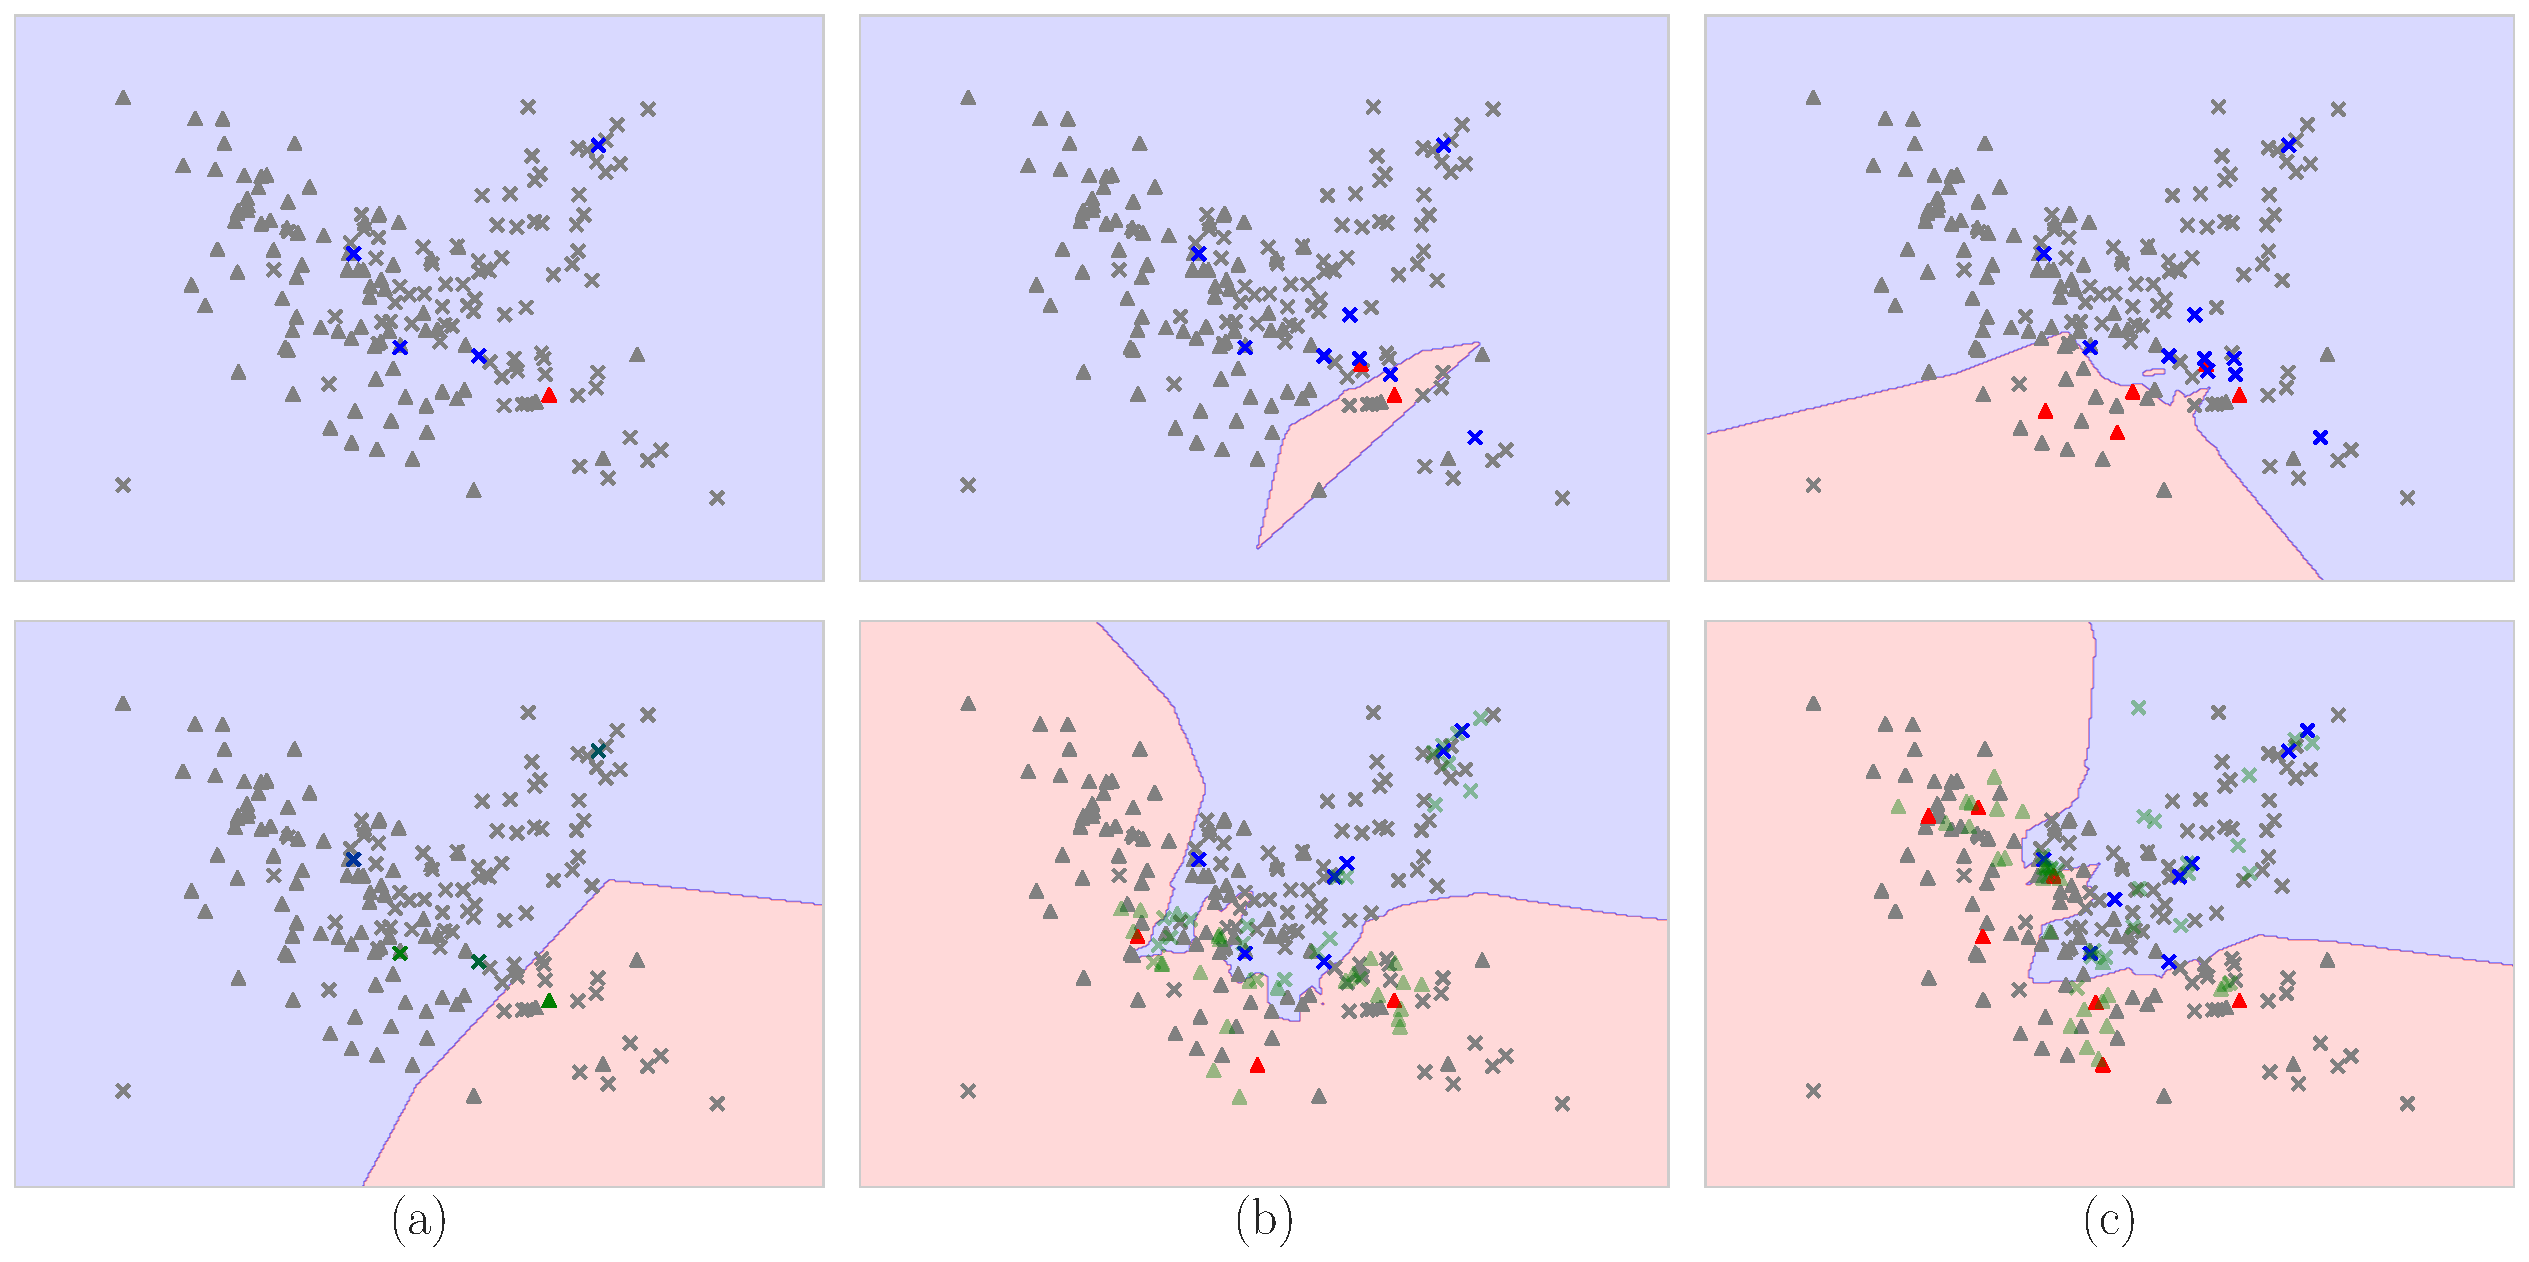
\includegraphics[width=\linewidth]{al-example}
    \caption[Illustration of the different acquisition processes in AL.]{%
        Illustration of the different acquisition processes in AL using a
        K-Nearest Neighbors classifier and Shannon's entropy as the
        uncertainty estimation function, with five observations being
        collected and labeled per iteration. The top row shows the behavior of
        a standard AL implementation, while the bottom row shows the behavior
        of the proposed method. Column (a), (b) and (c) show the decision
        boundaries at iterations 1 (after the collection of five random
        initial training observations), 2 (with 10 labeled observations) and 3
        (with 15 labeled observations), respectively. The initial labeled
        dataset for both approaches is the same. The two classes are
        distinguished with $\triangle$ and $\times$, and are colored as red
        and blue (respectively) if they are labeled. The transparent green
        observations are synthetic observations (bottow row only).
    }~\label{fig:al-example}
\end{figure}

Figure~\ref{fig:al-example} illustrates the difference across AL
iterations between the standard AL approach and the proposed method. Synthetic
data allowed for a quicker expansion of the labeled input area at an early
stage of the process, with better defined decision boundaries and
near-covergence of the ML classifier's performance at the third iteration.
Data augmentation influences the choice of unlabeled observations for labeling
into regions where synthetic data is not being able to represent the unlabeled
data pool.
 
\subsection{Motivation and contributions}

The usage of data augmentation in AL is not new. The literature found on the
topic (see Section~\ref{sec:data_augmentation_in_al-al-aug}) focuses on either image
classification or Natural Language Processing and uses Deep Learning-based
data augmentation to improve the performance of neural network architectures
in AL\@. These methods, although showing promising results, represent a
limited perspective of the potential of data augmentation in a real-world
setting: 

\begin{enumerate}

    \item Using Deep Learning in an iterative setting requires access to
        significant computational power.

    \item These models tend to use sophisticated data augmentation methods,
        whose implementation may not be accessible to non-sophisticated users.

    \item They require a significant amount of processing time per
        iteration and are inappropriate for settings with limited time
        budgets.

    \item The studies found on the topic are specific to the domain,
        classifier, and data augmentation method.
        In addition, all of the related methods found (except one) focus
        on either image or natural language processing classification
        problems.

\end{enumerate}

Consequently, the direct effect of data augmentation is unclear: these studies
implement different neural network-based techniques for different
classification problems, whose performance may be attributed to various
elements within the AL framework.

In this study, we explore the effect of data augmentation in AL in a
context-agnostic setting, along with two different data augmentation policies:
oversampling (where the amount of data generated for each class equals the
amount of data belonging to the majority class) and non-constant data
augmentation policies (where the amount of data generated exceeds the amount
of data belonging to the majority class in varying quantities) between
iterations. We start by conceptualizing the AL framework and each of its
elements, as well as the modifications involved to implement data augmentation
in the AL iterative process. We argue that simple, non-domain specific data
augmentation heuristics are sufficient to improve the performance of AL
implementations, without the need to resort to deep learning-based data
augmentation algorithms. These contributions can be summarized as
follows:

\begin{enumerate}

    \item We propose a flexible AL framework with pipelined data
        augmentation for tabular data that may be adapted for any domain or
        data type. This implementation is directed towards use cases with
        limited computational power and/or processing time.

    \item We use a geometric-based data augmentation method for
        non-network based classifiers and adapt it to leverage information
        from the AL process. To the best of our knowledge, most
        existing methods use domain/classifier-specific augmentations or the
        Mixup approach.

    \item We provide empirical evidence that the integration of varying data
        augmentation policies between iterations in the AL framework not only further
        reduces the amount of labeled data required, but is also a viable training
        strategy for fully supervised learning settings.

\end{enumerate}

When compared to the standard AL framework, the proposed framework contains
two additional components: the Generator and the Hyperparameter Optimizer. We
implement a modified version of the Geometric Synthetic Minority Oversampling
Technique (G-SMOTE)~\cite{Douzas2019} as a data augmentation method with an
optimized generation policy (explained in
Section~\ref{sec:data_augmentation}). We also propose a hyperparameter
optimization module, which is used to find the best data augmentation policy
at each iteration. We test the effectiveness of the proposed method in 15
datasets of different domains. We implement three AL frameworks (standard,
oversampling and varying data augmentation) using four different classifiers,
three different performance metrics and calculate two AL-specific performance
metrics. 

The remainder of this manuscript is structured as follows:
Section~\ref{sec:background-al-aug} introduces relevant topics discussed in the paper
and describes the related work. Section~\ref{sec:proposed_method-al-aug} elucidates
the proposed method. Section~\ref{sec:methodology-al-aug} details the methodology of
the study's experiment. Section~\ref{sec:results_discussion-al-aug} presents the
results obtained from the experiment, as well as a discussion of these
results. Section~\ref{sec:conclusion-al-aug} presents the conclusions drawn from
this study.
 
\section{Background}~\label{sec:background-al-aug}

In this section we describe the AL problem, data augmentation techniques, and review the
literature that combines AL with data augmentation. Table~\ref{tbl:generators}
describes the notations used throughout the rest of this study.

\begingroup\small
\begin{longtable}{clccccccc}
    \caption{%
        Description of all notations and symbols used throughout the
        manuscript.
    }\label{tbl:generators}\\
    \toprule
               Symbol & Meaning \\
    \midrule
    \endfirsthead%
    \caption[]{%
        Description of all notations and symbols used throughout the
        manuscript.
    } \\
    \toprule
               Symbol & Meaning \\
    \midrule
    \endhead%
    \midrule
    \multicolumn{9}{r}{{Continued on next page}} \\
    \midrule
    \endfoot%
    
    \bottomrule
    \endlastfoot%
               $f_{c}$ & ML classifier. \\
               $x_i$ & Observation at index $i$. \\
               $f_{acq}(x_i;f_c)$ & Acquisition function. \\
               $f_{aug}(x_i;\tau)$ & Augmentation function. \\
               $\tau$ & Augmentation policy. \\
               $\mathcal{D}$ & Data pool. Contains both labeled and unlabeled
                               data. \\
               $\mathcal{D}_{lab}^t$ & Labeled data set at iteration $t$. \\
               $\mathcal{D}_{pool}^t$ & Unlabeled data pool at iteration $t$. \\
               $\mathcal{D}_{new}^t$ & Set of observations from
                                       $\mathcal{D}_{pool}^t$to be labeled
                                       and added to $\mathcal{D}_{lab}^{t+1}$. \\
               $T$ & Iteration budget.\\
               $n$ & Annotation budget per iteration.\\
\end{longtable}
\endgroup


\subsection{Active Learning}~\label{sec:active_learning_methods-al-aug}

This paper focuses on pool-based AL methods as defined
in~\cite{katz2021improved}. The goal of AL models is to maximize the
performance of a classifier, $f_{c}$, while annotating as least observations,
$x_i$, as possible. They use a data pool, $\mathcal{D}$, where $\mathcal{D} =
\mathcal{D}_{lab} \cup \mathcal{D}_{pool}$ and $|\mathcal{D}_{pool}| \gg
|\mathcal{D}_{lab}|$. $\mathcal{D}_{pool}$ and $\mathcal{D}_{lab}$ refer to
the sets of unlabeled and labeled data, respectively. Having a budget of $T$
iterations (where $t \in \{1, 2, \ldots, T\}$) and $n$ annotations per iteration, at
iteration $t$, $f_c$ is trained using $\mathcal{D}_{lab}^t$ to produce, for
each $x_i \in \mathcal{D}_{pool}^t$, an uncertainty score using an acquisition
function $f_{acq}(x_i;f_c)$. These uncertainty scores are used to annotate the
$n$ observations with highest uncertainty from $\mathcal{D}_{pool}^t$ to form
$\mathcal{D}_{new}^t$. The iteration ends with the update of
$\mathcal{D}_{lab}^{t+1} = \mathcal{D}_{lab}^t \cup \mathcal{D}_{new}^t$ and
$\mathcal{D}_{pool}^{t+1} = \mathcal{D}_{pool}^t \setminus
\mathcal{D}_{new}^t$~\cite{Su2020, Sverchkov2017}. This process is shown in
Figure~\ref{fig:al_iteration}. Before the start of the iterative process,
assuming $\mathcal{D}_{lab}^{t=0} = \emptyset$, the data used to populate
$\mathcal{D}_{lab}^{t=1}$ is typically collected randomly from $\mathcal{D} =
\mathcal{D}_{pool}^{t=0}$ and is labeled by a supervisor~\cite{Fonseca2021al,
Yoo2019, Aghdam2019}. 

\begin{figure}[ht]
	\centering
	\includegraphics[width=.6\linewidth]{al_iteration}
    \caption[Diagram depicting a typical AL iteration.]{%
        Diagram depicting a typical AL iteration. In the first iteration, the
        training set collected during the initialization process becomes the
        ``Current Training Dataset''.
    }~\label{fig:al_iteration}
\end{figure}

Research focused on AL has typically been focused on the specification of
$f_{acq}$~\cite{hospedales2011finding} and domain-specific applications, such
as malware detection~\cite{li2022boosting} or Land Use/Land Cover
classification~\cite{li2020}. Acquisition functions can be divided into
two different categories~\cite{su2021cost, Kumar2020}: 

\begin{enumerate}

    \item Informative-based. These strategies use the classifier's output to
        assess the importance of each observation towards the performance of
        the classifier~\cite{Fu2013}.

    \item Representative-based. These strategies estimate the optimal set of
        observations that will optimize the classifier's
        performance~\cite{Kumar2020}.

\end{enumerate}

Although there are significant contributions toward the development of more
robust query functions and classifiers in AL, modifications to AL's basic
structure are rarely explored. In~\cite{Yoo2019} the authors introduce a loss
prediction module in the AL framework to replace the uncertainty criterion.
This model implements a second classifier to predict the expected loss of the
unlabeled observations (using the actual losses collected during the training
of the original classifier) and return the unlabeled observations with the
highest expected loss. However, this contribution is specific to deep neural
networks and was only tested for image classification.


%%%%%%%%%%%%%%%%%%%%%%%%%%%%%%%%%%%%%%%%%%%%%%%%%%%%%%%%%%%%%%%%%%%%%%%%%%%%%%

AL techniques may also be used to complement other well-known learning
challenges. For example, security bug report prediction tasks are typically
developed in imbalanced learning environment, where it is necessary to
manually label large amounts of data, which may result in mislabeled
data~\cite{wu2021data}. Another related example is machinery fault
diagnostics, where the quality and quantity of the data collected is often
recognized as a bottleneck~\cite{zhang2023blockchain}. In this case,
ML-based techniques frequently leverage unlabeled data to improve the
classification performance~\cite{zhang2021open} and rely on manual data
acquisition~\cite{he2017deep}. In these examples, the application of an
AL technique could reduce the amount of labeled data required, reduce the
strain in the supervisor's labeling process and reduce the amount of label
noise. 

An under explored challenge in the AL literature is the effective handling of
different data structures. One method to address this problem are autoencoder
architectures~\cite{li2017grass} or, in the case of text data, semantic
representation networks~\cite{zheng2021sentence}. However, understanding
how to integrate these two types of methods is a subject of future research.
Within other research streams, such as deep reinforcement learning, some
research also focus on optimizing observation efficiency during the learning
process~\cite{zhang2022training}.

%%%%%%%%%%%%%%%%%%%%%%%%%%%%%%%%%%%%%%%%%%%%%%%%%%%%%%%%%%%%%%%%%%%%%%%%%%%%%%

\subsection{Data Augmentation}~\label{sec:data_augmentation-al-aug}

The standard AL model can be complemented with a data augmentation function,
$f_{aug}(x_i;\tau)$, where $\tau$ defines the augmentation policy. In this
context, $\tau$ refers to the transformation applied and its hyperparameters
and $f_{aug}$ produces a modified observation, $\tilde{x} \in
\mathcal{D}_{aug}$ where $\mathcal{D}_{aug}$ is the set of modified
observations. This involves the usage of a new set of data,
$\mathcal{D}_{train}^t = \mathcal{D}_{lab}^t \cup \mathcal{D}_{aug}^t$, to
train the classifier.

Data Augmentation methods expand the training dataset by introducing new and
informative observations \cite{Behpour2019}. The production of artificial data
may be done via the introduction of perturbations on the
input~\cite{Fonseca2021}, feature~\cite{DeVries2017}, or output
space~\cite{Behpour2019}. Data Augmentation methods may be divided into two
categories~\cite{Shorten2019}:

\begin{enumerate}
    \item Heuristic approaches attempt to generate new and relevant
        observations by applying a predefined procedure, usually incorporating
        some degree of randomness~\cite{Kashefi2020}. Since these methods
        typically occur in the input space, they require fewer data and
        computational power when compared to Neural Network methods. 
    \item Neural Network approaches, on the other hand, map the original input
        space into a lower-dimensional representation, known as the feature
        space~\cite{DeVries2017}. The generation of artificial data occurs in
        the feature space and is reconstructed into the input space. Although
        these methods allow the generation of less noisy data in
        high-dimensional contexts and more plausible artificial data, they are
        significantly more computationally intensive. 
\end{enumerate}

While some techniques may depend on the domain, others are domain-agnostic.
For example, Random Erasing~\cite{Zhong2020}, Translation, Cropping and
Flipping are examples of image data-specific augmentation methods. Other
methods, such as autoencoders, may be considered domain agnostic.

\subsection{Data Augmentation in Active Learning
}~\label{sec:data_augmentation_in_al-al-aug}

% Pipelined approach
The only AL model found that uses data augmentation outside of the computer
vision or NLP domains implements a pipelined approach, described
in~\cite{Fonseca2021al}. In this study, the AL model proposed is applied for
tabular data using an oversampling data augmentation policy (\textit{i.e.},
the artificial data was only generated to balance the target class
frequencies). However, this AL model was applied in a Land Use/Land Cover
classification context with specific characteristics that are not necessarily
found in other supervised learning problems. Specifically, these types of
datasets are high dimensional and have limited data variability within each
class (\textit{i.e.,} cohesive spectral signatures within classes) due to
their geographical proximity. Furthermore, this method does not allow
augmentation policy optimization (i.e., every hyperparameter has to be
hard-coded \textit{a priori}).

The Bayesian Generative Active Deep Learning (BGDAL)~\cite{tran2019bayesian}
is another example of a pipelined combination of $f_{acq}$ and $f_{aug}$,
applied to image classification. BGDAL uses a Variational AutoEncoder (VAE)
architecture to generate artificial observations. However, the proposed model
is computationally expensive, requires a large data pool to train the VAE, and
is not only dependent on the quality of the augmentations performed, but also
on the performance of the discriminator and classifiers used.

% Look ahead data augmentation
The method proposed in~\cite{Kim2021}, Look-Ahead Data Acquisition for Deep
Active Learning, implements data augmentation to train a deep-learning
classifier. However, adapting existing AL applications to use this approach is
often impractical and implies the usage of image data since the augmentations
used are image data specific and occur on the unlabeled observations, before
the unlabeled data selection.

% VAE adversarial Active Learning (2019)
The Variational Adversarial Active Learning (VAAL)
model~\cite{sinha2019variational} is a deep AL approach to image
classification that uses as inputs the embeddings produced by a VAE into a
secondary classifier, working as $f_{acq}$, to predict if $x_i \in
\mathcal{D}$ belongs to $\mathcal{D}_{pool}$. The $n$ true positives with the
highest uncertainty are labeled by the supervisor and
$\mathcal{D}_{pool}$ and $\mathcal{D}_{lab}$ are updated as described in
Section~\ref{sec:active_learning_methods-al-aug}. The Task-aware VAAL
model~\cite{kim2021task} extends the VAAL model by introducing a ranker, which
consists of the Learning Loss module introduced in~\cite{Yoo2019}. These
models use data augmentation techniques to train the different neural
network-based components of the proposed models. However, the AL components
used are specific image classification, computationally expensive and the
analysis of the effect of data augmentation in these AL models is not
discussed.

% Other applications
In~\cite{Ma2020}, the proposed AL method was explicitly designed for image
data classification, where a deep learning model was implemented as a
classifier, but its architecture is not described, the augmentation policies
used are unknown and the results reported correspond to single runs of the
discussed model. The remaining AL models found implement data augmentation for
NLP applications, in~\cite{Quteineh2020, Li2021framework}. However, these
methods were designed for specific applications within that domain and are not
necessarily transferable to other domains or tasks.

\section{Proposed Method}~\label{sec:proposed_method-al-aug}

Based on the literature found on AL, most of the contributions and novel
implementations of AL algorithms have focused on the improvement of the
choice/architecture of the classifier or the improvement of the uncertainty
criterion. In addition, the resulting classification performance of AL-trained
classifiers is frequently inconsistent and marginally improve the
classification performance when compared to classifiers trained over the
entire training set. In addition, there is also significant variability in the
data selection efficiency during different runs of the AL iterative
process~\cite{Fonseca2021al}.
 
This paper provides a context-agnostic AL framework for the integration of
Data Augmentation within AL, with the following contributions:

\begin{enumerate}
    \item Improvement of the AL framework by introducing a parameter tuning
        stage only using the labeled dataset available at the current
        iteration (\textit{i.e.,} no labeled hold-out set is needed).
    \item Generalization of the generator module proposed in
        \cite{Fonseca2021al} from oversampling techniques to any other data
        augmentation mechanism and/or policy.
    \item Implementation of data augmentation outside the Deep AL realm, which
        was not previously found in the literature.
    \item Analysis of the impact of Data Augmentation and Oversampling in AL
        over 15 different datasets of different domains, while comparing them
        with the standard AL framework.
\end{enumerate}

The proposed AL framework is depicted in Figure~\ref{fig:al_proposed}. The
generator element becomes an additional source of data and is expected to
introduce additional data variability into the training dataset. This aspect
should allow the classifier to generalize better and perform more consistently
over unseen observations. However, in this scenario, the amount of data to
generate per class at each iteration is unknown. Consequently, the
hyperparameter tuning step was introduced to estimate the optimal data
augmentation policy at each iteration. In our implementation, this step uses
the current training dataset to perform an exhaustive search over specified
generator parameters, tested over a 5-fold cross-validation method. The best
augmentation policy found is used to train the iteration's classifier in the
following step. This procedure is described in
Algorithm~\ref{alg:al-framework}.


\begin{figure}
	\centering
	\includegraphics[width=.6\linewidth]{al_proposed}
    \caption[Diagram depicting the proposed AL iteration.]{%
        Diagram depicting the proposed AL iteration. The proposed
        modifications are comprised within the red polygon and marked
        with a boldface ``C.''
    }~\label{fig:al_proposed}
\end{figure}

We implemented a simple modification in the selection mechanism of the G-SMOTE
algorithm to show the effectiveness of data augmentation in an AL
implementation. We use the uncertainties produced by $f_{acq}$ to compute the
probabilities of observations to be selected for augmentation as an additional
parameter. This modification is described in Algorithm~\ref{alg:g-smote} 

\begin{algorithm}[ht]
    \SetKwInput{KwGiven}{Given}
    \SetKwProg{Fn}{Function}{:}{end}
    \caption{Proposed AL Framework (Single iteration)}\label{alg:al-framework}
    \DontPrintSemicolon%
    \KwGiven{$t \ge 1$, performance metric $f_{pm}$}
    \KwIn{$\mathcal{D}_{pool}$, $\mathcal{D}_{lab}$, $f_c$, $f_{aug}$,
    $f_{acq}$, $\tau_{grid}$, $k$, $n$}
    \KwOut{$\mathcal{D}_{pool}$, $\mathcal{D}_{lab}$}

    \Fn{ParameterTuning($f_c$, $f_{aug}$, $\tau_{grid}$, $\mathcal{D}_{lab}$,
    $k$)}{
        $p \leftarrow 0$ \\
        $\tau \leftarrow \emptyset$ \\
        $\{\mathcal{D}_{lab}^1, \ldots \mathcal{D}_{lab}^k\} \leftarrow
        \mathcal{D}_{lab}$
        \tcp*[f]{$\mathcal{D}_{lab}^n \cap \mathcal{D}_{lab}^m = \emptyset,
        \forall (n, m) \in {1, \ldots, k}$} \\
        \ForAll{$\tau' \in \tau_{grid}$}{
            $p' \leftarrow \emptyset$ \\
            \ForAll{
                $\mathcal{D}_{lab}^i \in \{\mathcal{D}_{lab}^1, \ldots
                \mathcal{D}_{lab}^k\}$
            }{
                $\mathcal{D}_{test}' \leftarrow \mathcal{D}_{lab}^i$ \\
                $\mathcal{D}_{train}' \leftarrow \mathcal{D}_{lab} \setminus
                \mathcal{D}_{lab}^i$ \\
                $\mathcal{D}_{train}' \leftarrow f_{aug}(\mathcal{D}_{train}';
                \tau')$ \\
                \textbf{train} $f_c$ using $\mathcal{D}_{train}'$ \\
                $p' \leftarrow p' \cup \{f_{pm}(f_c(\mathcal{D}_{test}))\}$
            }
            $p' \leftarrow \frac{\sum_{x_i \in p'}{x_i}}{k}$ \\
            \If{$p' > p$}{
                $p \leftarrow p'$ \\
                $\tau \leftarrow \tau'$
            }
        }
        \Return $\tau$
    }

    \Begin{
        $\tau \leftarrow ParameterTuning(f_c, f_{aug}, \tau_{grid},
        \mathcal{D}_{lab}, k)$ \\
        $\mathcal{D}_{train} \leftarrow f_{aug}(\mathcal{D}_{lab}; \tau)$ \\
        \textbf{train} $f_c$ using $\mathcal{D}_{train}$ \\
        $\mathcal{D}_{new} = \arg\max_{\mathcal{D}_{pool}'\subset
        \mathcal{D}_{pool}, |\mathcal{D}_{pool}'|=n} \sum_{x \in
        \mathcal{D}_{pool}'}{f_{acq}(x; f_c)}$ \\
        \textbf{annotate} $\mathcal{D}_{new}$ \\
        $\mathcal{D}_{pool} \leftarrow \mathcal{D}_{pool} \setminus
        \mathcal{D}_{new}$ \\
        $\mathcal{D}_{lab} \leftarrow \mathcal{D}_{lab} \cup
        \mathcal{D}_{new}$ \\
    }

\end{algorithm}

This modification facilitates the usage of G-SMOTE beyond its original
oversampling purposes. However, in this paper, the data augmentation
strategies are also used to ensure that class frequencies are balanced.
Furthermore, the amount of artificial data produced for each class is defined
by the \textit{augmentation factor}, $\alpha_{af}$, which represents a
percentage of the majority class $C_{maj}$ (\textit{e.g.,} an augmentation
factor of $1.2$ will ensure there are $count(C_{maj}) \times 1.2$ observations
in every class). In this paper's experiment, the data generation mechanism is
similar to the one in~\cite{Fonseca2021al}. This factor allows the direct
comparison of the two frameworks and establishes a causality of the
performance variations to the data generation mechanism (\textit{i.e.,}
augmentation vs normal oversampling) and hyperparameter tuning steps.
However, in this case, the hyperparameter tuning is solely going to be used
for augmentation policy optimization. 

\begin{algorithm}[t]
    \SetKwInput{KwGiven}{Given}
    \SetKwProg{Fn}{Function}{:}{end}
    \caption{G-SMOTE Modified for Data Augmentation in AL}\label{alg:g-smote}
    \DontPrintSemicolon% 
    \KwGiven{$t \ge 1$, $\mathcal{D}_{lab}^t \ne \emptyset$,
    $\mathcal{D}_{lab} = \mathcal{D}_{lab}^{min} \cup \mathcal{D}_{lab}^{maj}$, \textit{GSMOTE}}
    \KwIn{$\mathcal{D}_{pool}^t$, $\mathcal{D}_{lab}^t$, $f_c^{t-1}$,
    $f_{acq}$, $\tau$}
    \KwOut{$\mathcal{D}_{train}^t$}

    \Fn{DataSelection($\mathcal{D}_{lab}^t$, $f_{acq}$, $f_c^{t-1}$)}{%
        $U \leftarrow \emptyset$ \\ 
        $P \leftarrow \emptyset$ \\ 
        $p_s \sim \mathcal{U}(0, 1)$ \\
        \ForAll{$x_i \in \mathcal{D}_{lab}^t$}{
            $u_{x_i} \leftarrow f_{acq}(x_i; f_c^{t-1})$\\
            $U \leftarrow U \cup \{u_{x_i}\}$
        }
        \ForAll{$u_{x_i} \in U$}{
            $p_{x_i} \leftarrow \frac{u_{x_i}}{\sum{U}} + \sum{P}$ \\
            $P \leftarrow P \cup \{p_{x_i}\}$
        }
        $i \leftarrow argmax(P < p_s)$ \\
        \Return i-th element in $\mathcal{D}_{lab}^t$
    }
    \Begin{
        $\mathcal{D}_{aug}^{min} \leftarrow \emptyset$ \\
        $\mathcal{D}_{aug}^{maj} \leftarrow \emptyset$ \\
        $\alpha_{af}, \alpha_{trunc}, \alpha_{def} \leftarrow \tau$ \\
        $N \leftarrow count(C_{maj}) \times \alpha_{af}$ \\
        
        \ForAll{
            $\mathcal{D}'_{aug} \in \{\mathcal{D}_{aug}^{min},
            \mathcal{D}_{aug}^{maj}\}$, $\mathcal{D}'_{lab} \in \{\mathcal{D}_{lab}^{min},
            \mathcal{D}_{lab}^{maj}\}$
        }{
            \While{
                $|\mathcal{D}'_{aug}| < N$
            }{
                $x_{center} \leftarrow DataSelection(\mathcal{D}'_{lab},
                f_{acq}, f_c^{t-1})$ \\
                $x_{gen} \leftarrow GSMOTE(x_{center}, \mathcal{D}_{lab}^t, \alpha_{trunc},
                \alpha_{def})$ \\
                $\mathcal{D}'_{aug} \leftarrow \mathcal{D}'_{aug} \cup
                \{x_{gen}\}$
            }
        }
        $\mathcal{D}_{aug} \leftarrow \mathcal{D}_{aug}^{min} \cup \mathcal{D}_{aug}^{maj}$ \\
        $\mathcal{D}_{train}^t \leftarrow \mathcal{D}_{lab}^t \cup
        \mathcal{D}_{aug}$
    }
\end{algorithm}

In the proposed framework, we (1) generalize the generator module to accept
any data augmentation method or policy and (2) introduce a hyperparameter
tuning module to estimate the optimal data augmentation policy. This framework
was designed to be task-agnostic. Specifically, any data augmentation method
(domain-specific or not) may be applied, as well as any other parameter search
method. It is also expected to be compatible with other AL modifications,
including those that do not affect solely the classifier or uncertainty
criterion, such as the one proposed in~\cite{Yoo2019}.
 
\section{Methodology}~\label{sec:methodology-al-aug}

This section describes the different elements included in the experimental
procedure. The datasets used were acquired in open data repositories. Their
sources and preprocessing steps are defined in
Subsection~\ref{sec:datasets-al-aug}.
The classifiers used in the experiment are defined in
Subsection~\ref{sec:machine_learning_algorithms-al-aug}. The metrics chosen to
measure AL performance and overall classification performance are defined in
Subsection~\ref{sec:evaluation_metrics-al-aug}. The experimental procedure is
described in Subsection~\ref{sec:experimental_procedure-al-aug}.

The methodology developed serves a two-fold purpose: (1) Compare
classification performance once all the AL procedures are completed
(\textit{i.e.,} optimal performance of a classifier trained via iterative data
selection) and (2) Compare the amount of data required to reach specific
performance thresholds (\textit{i.e.,} the number of AL iterations required to
reach similar classification performances).
 
\subsection{Datasets}~\label{sec:datasets-al-aug}

The datasets used to test the proposed method are publicly available in open
data repositories. Specifically, they were retrieved from the OpenML and the
UCI Machine Learning Repository websites. They were chosen considering diverse
application domains, imbalance ratios, dimensionality and number of target
classes, all of them focused on classification tasks. The goal is to
demonstrate the performance of the different AL frameworks in various
scenarios and domains. The data preprocessing approach was similar across all
datasets.  Table~\ref{tab:datasets_description} describes the key properties
of the 15 preprocessed datasets where the experimental procedure was applied. 
 
\begin{table}
    \centering
    \setlength{\tabcolsep}{2pt}
    \caption[Description of the datasets collected after data preprocessing.
    ]{%
        \label{tab:datasets_description}
        Description of the datasets collected after data preprocessing. The
        sampling strategy is similar across datasets. Legend: (IR) Imbalance
        Ratio
    }
    \pgfplotstabletypeset[
        col sep=comma,
        string type,
        every head row/.style={%
            before row=\toprule,
            after row=\midrule
        },
        every last row/.style={after row=\bottomrule},
    ]{figures/active-learning-augmentation/datasets_description.csv}
\end{table}

The data preprocessing pipeline is depicted as a flowchart in
Figure~\ref{fig:data_preprocessing}. The missing values are removed from each
dataset by removing the corresponding observations. This step ensures that the
input data in the experiment is kept as close to its original form as
possible. The non-metric features (\textit{i.e.,} binary, categorical, and
ordinal variables) were removed since the application of G-SMOTE is limited to
continuous and discrete features. The datasets containing over 2000
observations were downsampled in order to maintain the datasets to a
manageable size. The data sampling procedure preserves the relative class
frequency of the dataset, in order to maintain the Imbalance Ratio (IR)
originally found in each dataset (where $IR =
\frac{count(C_{maj})}{count(C_{\min})}$). The remaining features of each
dataset are scaled to the range of $[-1, 1]$ to ensure a common range across
features.

\begin{figure}[t]
	\centering
	\includegraphics[width=.8\linewidth]{data_preprocessing}
    \caption{%
        Data preprocessing pipeline.
    }~\label{fig:data_preprocessing}
\end{figure}

The preprocessed datasets were stored into an SQLite database file and is
available along with the experiment's source code in the project's GitHub
repository (see final remarks regarding data and software availability).
 
\subsection{Machine Learning Algorithms}~\label{sec:machine_learning_algorithms-al-aug}

We used a total of four classification algorithms and a heuristic data
augmentation mechanism. The choice of classifiers was based on the popularity
and family of the classifiers (tree-based, nearest neighbors-based,
ensemble-based and linear models). Our proposed method was tested using a
Decision Tree (DT)~\cite{Wu1975}, a K-nearest neighbors classifier
(KNN)~\cite{Cover1967}, a Random Forest Classifier (RF)~\cite{Ho1995} and a
Logistic Regression (LR)~\cite{Nelder1972}. Since the target variables are
multi-class, the LR classifier was implemented using the one-versus-all
approach. The predicted class is assigned to the label with the highest
likelihood.
 
The oversampler G-SMOTE was used as a data augmentation method. The typical
data generation policy of oversampling methods is to generate artificial
observations on non-majority classes such that the number of majority class
observations matches those of each non-majority class. We modified this data
generation policy to generate observations for all classes, as a percentage of
the number of observations in the majority class. In addition, the original
G-SMOTE algorithm was modified to accept data selection probabilities based on
classification uncertainty. These modifications are discussed in
Section~\ref{sec:proposed_method-al-aug}.

Every AL procedure was tested with different selection criteria: Random
Selection, Entropy, and Breaking Ties. The baseline used is the standard AL
procedure. As a benchmark, we add the AL procedure using G-SMOTE as a standard
oversampling method, as proposed in~\cite{Fonseca2021al}. Our proposed method
was implemented using G-SMOTE as a data augmentation method to generate
artificial observations for all classes, while still balancing the class
distribution, as described in Section~\ref{sec:proposed_method-al-aug}. 
 
\subsection{Evaluation Metrics}~\label{sec:evaluation_metrics-al-aug}

Considering the imbalanced nature of the datasets used in the experiment,
commonly used performance metrics such as Overall Accuracy (OA), although
being intuitive to interpret, are insufficient to quantify a model's
classification performance~\cite{Jeni2013}. The Cohen's Kappa performance
metric, similar to OA, is also biased towards high-frequency classes since its
definition is closely related to the OA metric, making its behavior consistent
with OA~\cite{Fatourechi2008}. However, these metrics remain popular choices
for the evaluation of classification performance. Other performance metrics
like $Precision = \frac{TP}{TP+FP}$, $Recall = \frac{TP}{TP+FN}$ (also
known as Sensitivity) or $Specificity = \frac{TN}{TN + FP}$ are calculated as
a function of True/False Positives (TP and FP) and True/False Negatives (TN
and FN) and can be used on a per-class basis instead. In a multiple dataset
scenario with varying amounts of target classes and meanings, comparing the
performance of different models using these metrics becomes impractical.
 
Based on the recommendations found in~\cite{Jeni2013, Kubat1997}, we used two
metrics found to be less sensitive to the class imbalance bias, along with OA
as a reference for easier interpretability:

\begin{itemize}
    \item The Geometric-mean scorer (G-mean) consists of the geometric mean of
        Specificity and Recall~\cite{Kubat1997}. Both metrics are calculated
        in a multi-class context considering a one-versus-all approach. For
        multi-class problems, the G-mean scorer is calculated as its average
        per class values: 
        
        \begin{equation*}
            \textit{G-mean} = \sqrt{\overline{Recall} \times
            \overline{Specificity}}
        \end{equation*}

    \item The F-score metric consists of the harmonic mean of Precision and
        Recall. The two metrics are also calculated considering a
        one-versus-all approach. The F-score for the multi-class case can be
        calculated using its average per class values~\cite{Jeni2013}:

        \begin{equation*}
            \textit{F-score}=2\times\frac{\overline{Precision} \times
            \overline{Recall}}{\overline{Precision} + \overline{Recall}}
        \end{equation*}

    \item The OA consists of the number of TP divided by the total amount of
        observations. Considering $c$ as the label for the different classes
        present in a target class, OA is given by the following formula:

        \begin{equation*}
            \textit{OA} = \frac{\sum\limits_{c}{\text{TP}_{c}}}{%
		    	      \sum\limits_{c}{(\text{TP}_{c}+\text{FP}_{c})}}
        \end{equation*}
\end{itemize}

The comparison of the performance of AL frameworks is based on its data
selection and augmentation efficacy. Specifically, an efficient data
selection/generation policy allows the production of classifiers with high
performance on unseen data while using as least non-artificial training data
as possible. We follow the recommendations found in~\cite{Kottke2017}. To
measure the performance of the different AL setups, the performance of an AL
setup will be compared using two AL-specific performance metrics:

\begin{itemize}

    \item Area Under the Learning Curve (AULC). It is the sum of the
        classification performance over a validation/test set of the
        classifiers trained of all AL iterations. The resulting AULC scores
        are fixed within the range $[0, 1]$ by dividing the AULC scores by the
        total amount of iterations (\textit{i.e.}, the maximum performance
        area) to facilitate the interpretability of this metric.

    \item Data Utilization Rate (DUR)~\cite{Reitmaier2013}. Measures the
        percentage of training data required to reach a given performance
        threshold, as a ratio of the percentage of training data required by
        the baseline framework. This metric is also presented as a percentage
        of the total amount of training data, without making it relative to
        the baseline framework. The DUR metric is measured at 45 different
        performance thresholds, ranging between $[0.10, 1.00]$ at a 0.02 step.

\end{itemize}
 
\subsection{Experimental Procedure}~\label{sec:experimental_procedure-al-aug}

The evaluation of different active learners in a live setting is generally
expensive, time-consuming, and prone to human error. Instead, a common
practice is to compare them in an offline environment using labeled
datasets~\cite{Kagy2019}. Since the dataset is already labeled, the annotation
process is done at zero cost in this scenario.
Figure~\ref{fig:experimental_procedure} depicts the experiment designed for
one dataset over a single run. 
 
A single run starts with the splitting of a preprocessed dataset into five
different partitions, stratified according to the class frequencies of the
target variable using the K-fold Cross Validation method. During this run, an
active learner or classifier is trained five times using a different partition
as the Test set each time. For each training process, a validation set
containing 25\% of the subset is created and is used to measure the data
selection efficiency (\textit{i.e.,} AULC and DUR using the classification
performance metrics, specific to AL). Therefore, for a single training
procedure, 20\% of the original dataset is used as the validation set, 20\% is
used as the Test set and 60\% is used as the training set. The AL simulations
and the classifiers' training occur within the training set. However, the
classifiers used to find the maximum performance classification scores are
trained over the full training set. The AL simulations are run over a maximum
of 50 iterations (including the initialization step), adding 1.6\% of the
training set each time (\textit{i.e.,} all AL simulations use less than 80\%
of the training set). Once the training phase is completed, the Test set
classification scores are calculated using the trained classifiers. For the
case of AL, the classifier with the optimal validation set score is used to
estimate the AL's optimal classification performance over unseen data.

The process shown in Figure~\ref{fig:experimental_procedure} is repeated over
three runs using different random seeds over the 15 different datasets
collected. The final scores of each AL configuration and classifier correspond
to the average of the three runs and 5-fold Cross-Validation estimations
(\textit{i.e.,} the mean score of 15 fits, across 15 datasets).

\begin{figure}
	\centering
	\includegraphics[width=.6\linewidth]{experimental_procedure}
    \caption[Experimental procedure flowchart.]{%
        Experimental procedure flowchart. The preprocessed datasets are split
        into five folds. One of the folds is used to test the best-found
        classifiers using AL and the classifiers trained using the entire
        training dataset (containing the remaining folds). The training set is
        used to run both the AL simulations as well as train the normal
        classifiers. The validation set is used to measure AL-specific
        performance metrics over each iteration. We use different subsets for
        overall classification performance and AL-specific performance to
        avoid data leakage.
    }~\label{fig:experimental_procedure}
\end{figure}

The hyperparameters defined for the AL frameworks, Classifiers, and Generators
are shown in Table~\ref{tab:grid}. In the Generators table, we distinguish the
G-SMOTE algorithm working as a normal oversampling method from G-SMOTE-AUGM,
which generates additional artificial data on top of the usual oversampling
mechanism. Since the G-SMOTE-AUGM method is intended to be used with varying
parameter values (via within-iteration parameter tuning), the parameters were
defined as a list of various possible values. The remaining parameters
were selected based on knowledge gathered in previous literature and
typical default values for each of the algorithms. This choice was motivated
by the impossibility of parameter tuning in a real-world setting when applying
the benchmark AL methods. Although the proposed method addresses this
limitation, we show that exclusively tuning the parameters on the augmentation
policy is already sufficient to achieve superior, statistically significant
performance.

\begin{table}
	\centering
    \caption{\label{tab:grid}
        Hyperparameter definition for the active learners, classifiers,
        and generators used in the experiment.
    }
	\begin{tabular}{lll}
		\toprule
		Active Learners & Hyperparameters                   & Inputs                         \\
		\midrule
		Standard        & \# initial obs.\                  & 1.6\%                          \\
                        & \# additional obs.\ per iteration & 1.6\%                          \\
                        & max.\ iterations + initialization & 50                             \\
                        & evaluation metrics                & G-mean, F-score, OA            \\
                        & selection strategy                & Random, Entropy, Breaking Ties \\
                        & within-iteration param.\ tuning   & None                           \\
                        & generator                         & None                           \\
                        & classifier                        & DT, LR, KNN, RF                \\
        Oversampling    & generator                         & G-SMOTE                        \\
        Proposed        & generator                         & G-SMOTE-AUGM                   \\
                        & within-iteration param.\ tuning   & Grid Search K-fold CV          \\
		\toprule
		Classifier      &                                  &                                \\
		\midrule
        DT              & min.\ samples split              & 2                              \\
                        & criterion                        & gini                           \\
		LR              & maximum iterations               & 100                            \\
                        & multi-class                      & One-vs-All                     \\
		                & solver                           & liblinear                      \\
                        & penalty                          & L2 (Ridge)                     \\
		KNN             & \# neighbors                     & 5                              \\
                        & weights                          & uniform                        \\
                        & metric                           & euclidean                      \\
		RF              & min.\ samples split              & 2                              \\
		                & \# estimators                    & 100                            \\
                        & criterion                        & gini                           \\
		\toprule
		Generator       &                                  &                                \\
		\midrule
		G-SMOTE         & \# neighbors                     & 4                              \\
                        & deformation factor               & 0.5                            \\
                        & truncation factor                & 0.5                            \\
		G-SMOTE-AUGM    & \# neighbors                     & 3, 4, 5                        \\
                        & deformation factor               & 0.5                            \\
                        & truncation factor                & 0.5                            \\
                        & augmentation factor              & $[1.1, 2.0]$ at 0.1 step       \\
		\bottomrule
	\end{tabular}
\end{table}
 
\subsection{Software Implementation}~\label{sec:software_implementation}

The experiment was implemented using the Python programming language, along
with the Python libraries
\href{https://scikit-learn.org/stable/}{Scikit-Learn}~\cite{Pedregosa2011},
\href{https://imbalanced-learn.org/en/stable/}{Imbalanced-Learn}~\cite{JMLR:v18:16-365},
\href{https://geometric-smote.readthedocs.io/en/latest/?badge=latest}{Geometric-SMOTE}~\cite{Douzas2019},
\href{https://research-learn.readthedocs.io/en/latest/?badge=latest}{Research-Learn}
and
\href{https://mlresearch.readthedocs.io/en/latest/?badge=latest}{ML-Research}
libraries. All functions, algorithms, experiments, and results are provided in
the \href{https://github.com/joaopfonseca/publications/}{project's GitHub
repository}. The original datasets used in this study are publicly available
in open data repositories. They were retrieved from OpenML and the UCI Machine
Learning Repository. 

\section{Results \& Discussion}~\label{sec:results_discussion-al-aug}

In a multiple dataset experiment, the analysis of results should not rely upon
the average performance scores across datasets uniquely. The domain of
application and fluctuations of performance scores between datasets make the
analysis of these averaged results less accurate. Instead, it is generally
recommended to use the mean ranking scores to extend the
analysis~\cite{Demsar2006}. Since mean performance scores are still intuitive
to interpret; we will present and discuss both results. The rank values are
assigned based on the mean scores of three different 5-fold Cross-Validation
runs (15 performance estimations per dataset) for each combination of dataset,
AL configuration, classifier, and performance metric.
 
\subsection{Results}~\label{sec:results-al-aug}

The average rankings of the AL methods' AULC estimations are shown in
Table~\ref{tab:aulc_ranks}. The proposed method almost always improves AL
performance and ensures higher data selection efficiency.
 
\begin{table}[ht]
	\centering
    \caption[Mean rankings of the AULC metric over the different datasets (15),
        folds (5), and runs (3) used in the experiment.]{%
        Mean rankings of the AULC metric over the different datasets (15),
        folds (5), and runs (3) used in the experiment. The proposed method
        constantly improves the results of the original framework and, on
        average, almost always improves the results of the oversampling
        framework.
    }\label{tab:aulc_ranks}
    \pgfplotstabletypeset[
        col sep=comma,
        string type,
        every head row/.style={%
            before row=\toprule,
            after row=\midrule
        },
        every last row/.style={after row=\bottomrule},
    ]{figures/active-learning-augmentation/mean_std_aulc_ranks.csv}
\end{table}
 
Table~\ref{tab:aulc_scores} shows the average AULC scores, grouped by the
classifier, Evaluation Metric and AL framework. The performance of the
proposed method is almost always superior when considering the F-score and
G-mean. On some occasions, the average AULC score is significantly improved
when compared with the oversampling AL method.

\begin{table}
	\centering
    \setlength{\tabcolsep}{2.5pt}
    \caption[Average AULC of each AL configuration tested.]{%
        \label{tab:aulc_scores}
        Average AULC of each AL configuration tested. Each AULC score is
        calculated using the performance scores of each iteration in the
        validation set. By the end of the iterative process, each AL
        configuration used a maximum of 80\% instances of the 60\% instances
        that compose the training sets (\textit{i.e.,} 48\% of the entire
        preprocessed dataset).
    }
    \pgfplotstabletypeset[
        col sep=comma,
        string type,
        every head row/.style={%
            before row=\toprule,
            after row=\midrule
        },
        every last row/.style={after row=\bottomrule},
    ]{figures/active-learning-augmentation/mean_std_aulc_scores.csv}
\end{table}

The average DUR scores were calculated for various G-mean thresholds, varying
between 0.1 and 1.0 at a 0.02 step (45 different thresholds in total).
Table~\ref{tab:optimal_data_utilization} shows the results obtained for these
scores starting from a G-mean score of 0.6 and was filtered to show the
thresholds ending with 0 or 6 only. In most cases, the proposed method reduces
the amount of data annotation required to reach each G-mean score threshold.

\begin{table}[t]
    \centering
    \setlength{\tabcolsep}{2.5pt}
    \caption{\label{tab:optimal_data_utilization}
        AL algorithms' mean data utilization as a percentage of the
        training set.
    }
    \pgfplotstabletypeset[
        col sep=comma,
        string type,
        every head row/.style={%
            before row=\toprule,
            after row=\midrule
        },
        every last row/.style={after row=\bottomrule},
    ]{figures/active-learning-augmentation/optimal_data_utilization.csv}
\end{table}

The DUR scores relative to the Standard AL method are shown in
Figure~\ref{fig:dur}. A DUR below 1 means that the Proposed/Oversampling
method requires less data than the Standard AL method to reach the same
performance threshold. For example, running an AL simulation using the KNN
classifier requires 80.7\% of the amount of data required by the Standard AL
method using the same classifier to reach an F-Score of 0.62 (\textit{i.e.,}
requires 19.3\% less data).

\begin{figure}[t]
	\centering
	\includegraphics[width=.8\linewidth]{data_utilization_rate}
    \caption[Mean data utilization rates.]{%
        Mean data utilization rates. The y-axis shows the percentage of data
        (relative to the baseline AL framework) required to reach the
        different performance thresholds.
    }~\label{fig:dur}
\end{figure}

The comparison of mean optimal classification scores of AL methods with
Classifiers (using the entire training set, without AL) is shown in
Table~\ref{tab:optimal_mean_std_scores}. Aside from the case of overall
accuracy, the proposed AL method produces classifiers that almost consistently
outperform classifiers using the whole training set (\textit{i.e.,} the ones
labeled as MP).

\begin{table}
    \centering
    \caption[Optimal classification scores.]{%
        \label{tab:optimal_mean_std_scores}
        Optimal classification scores. The Maximum Performance (MP)
        classification scores are calculated using classifiers trained using
        the entire training set.
    }
    \pgfplotstabletypeset[
        col sep=comma,
        string type,
        every head row/.style={%
            before row=\toprule,
            after row=\midrule
        },
        every last row/.style={after row=\bottomrule},
    ]{figures/active-learning-augmentation/optimal_mean_std_scores.csv}
\end{table}

\subsection{Statistical Analysis}~\label{sec:statistical-analysis-al-aug}

When checking for statistical significance in a multiple dataset context it is
critical to account for the multiple comparison problem. Consequently, our
statistical analysis focuses on the recommendations found
in~\cite{Demsar2006}. Overall, we perform three statistical tests. The
Friedman test~\cite{Friedman1937} is used to understand whether there is a
statistically significant difference in performance between the three AL
frameworks. As \textit{post hoc} analysis, the Wilcoxon signed-rank
test~\cite{Wilcoxon1945} was utilized to check for statistical significance
between the performance of the proposed AL method and the oversampling AL
method across datasets. As a second \textit{post hoc} analysis, the
Holm-Bonferroni~\cite{Holm1979} method was employed to check for statistical
significance between the methods using data generators and the Standard AL
framework across classifiers and evaluation metrics.
 
Table~\ref{tab:friedman_test} displays the \textit{p-values} obtained with the
Friedman test. The difference in performance across AL frameworks is
statistically significant at a level of $\alpha = 0.05$ regardless of the
classifier or evaluation metric being considered.

\begin{table}[t]
	\centering
    \caption[Friedman test results.]{%
        Friedman test results. Statistical significance is tested at a level
        of $\alpha = 0.05$. The null hypothesis is that there is no difference
        in the classification outcome across oversamplers.
    }\label{tab:friedman_test}
    \pgfplotstabletypeset[
        col sep=comma,
        string type,
        every head row/.style={%
            before row=\toprule,
            after row=\midrule
        },
        every last row/.style={after row=\bottomrule},
    ]{figures/active-learning-augmentation/friedman_test.csv}
\end{table}

Table~\ref{tab:wilcoxon_test_al_aug} contains the \textit{p-values} obtained with the
Wilcoxon signed-rank test. The proposed method was able to outperform both the
standard AL framework, as well as the AL framework using a typical
oversampling policy with statistical significance in 14 and 12 out of 15
datasets, respectively.

\begin{table}
	\centering
    \caption[Adjusted p-values using the Wilcoxon signed-rank method.]{%
        Adjusted p-values using the Wilcoxon signed-rank method. Bold values
        are statistically significant at a level of $\alpha = 0.05$. The null
        hypothesis is that the performance of the proposed framework is
        similar to that of the oversampling or standard framework.
    }\label{tab:wilcoxon_test_al_aug}
    \pgfplotstabletypeset[
        col sep=comma,
        string type,
        every head row/.style={%
            before row=\toprule,
            after row=\midrule
        },
        every last row/.style={after row=\bottomrule},
    ]{figures/active-learning-augmentation/wilcoxon_test.csv}
\end{table}

The \textit{p-values} shown in Table~\ref{tab:holms_test} refer to the results
of the Holm-Bonferroni test. The proposed method's superior performance was
statistically significant in 9 out of 12 cases. 

\begin{table}
	\centering
    \caption[Adjusted p-values using the Holm-Bonferroni method.]{%
        Adjusted p-values using the Holm-Bonferroni method. Bold values are
        statistically significant at a level of $\alpha = 0.05$. The null
        hypothesis is that the Oversampling or Proposed method does not
        perform better than the control method (Standard AL framework).
    }\label{tab:holms_test}
    \pgfplotstabletypeset[
        col sep=comma,
        string type,
        every head row/.style={%
            before row=\toprule,
            after row=\midrule
        },
        every last row/.style={after row=\bottomrule},
    ]{figures/active-learning-augmentation/holms_test.csv}
\end{table}

\subsection{Discussion}~\label{sec:sub_discussion-al-aug}

In this paper, we study the application of data augmentation methods through
the modification of the standard AL framework. This is done to further reduce
the amount of labeled data required to produce a reliable classifier, at the
expense of artificial data generation. Overall, the proposed method
achieves better and more consistent performance when compared to the remaining
benchmark approaches. It was implemented to focus on the optimization of the
data augmentation policy, as well as the introduction of a more informed
AL-based data augmentation approach. The proposed method could be further
extended and achieve an even higher performance by optimizing parameters of
the ML classification using the hyperparameter optimizer. In addition, this
framework could be further generalized by searching, within AL iterations, for
the optimal ML classifier as well; at different stages of the data collection
procedure some ML classifiers might be more useful than others. Although the
proposed framework significantly improves the flexibility of AL
implementations, we found that even a superficial parameter search is
sufficient to ensure a superior performance when compared to related
approaches.
 
% a different data generation strategy
% - Superiority of AL proposed vs standard (AULC + statistical analysis)
In Table~\ref{tab:aulc_ranks}, we found that the proposed method was able to
outperform the Standard AL framework in all scenarios. Except for the overall
accuracy metric, the mean rankings are consistent with the mean AULC scores
found in Table~\ref{tab:aulc_scores}, while showing performance improvements
between the proposed method and both the standard and oversampling methods.
The Friedman test in Table~\ref{tab:friedman_test} showed that the difference
in the performance of these AL frameworks are statistically significant,
regardless of the classifier or performance metric being used.
 
% parameter optimization within the iterative process of an AL procedure
% - Discuss consistency of results as compared with other methods (DUR metric)
The proposed method evidenced more consistent data utilization requirements in
most of the assessed G-mean score thresholds when compared to the remaining AL
methods, as seen in Table~\ref{tab:optimal_data_utilization}. For example, to
reach a G-mean score of 0.9 using the KNN and LR classifiers, the average
amount of data required with the Oversampling AL approach increased when
compared to the standard approach. However, the proposed method was able to
decrease the amount of data required in both situations. The robustness of the
proposed method is clearer in Figure~\ref{fig:dur}. In most cases, this method
was able to outperform the Oversampling method. At the same time, the proposed
method also addresses inconsistencies in situations where the Oversampling
method was unable to outperform the standard method.

% Data augmentation vs oversampling
The statistical analyses found in Tables~\ref{tab:wilcoxon_test_al_aug}
and~\ref{tab:holms_test} revealed that the proposed method's superiority was
statistically significant in all datasets except three (Baseball, Usps, and
Volkert) and established statistical significance when compared to the
standard AL method for all combinations of classifier and performance metric,
except for three cases regarding the use of the overall accuracy metric. These
results show that the proposed method increased the reliability of the new AL
framework and improved the quality of the final classifier while using fewer
data.

% Usage of AL as a method to produce better performing classifiers, even in
% settings with fully labeled data
Even though it was not the core purpose of this study, we found that the
proposed AL method consistently outperformed the maximum performance
threshold. Specifically, in Table~\ref{tab:optimal_mean_std_scores}, the
performance of the classifiers originating from the proposed method was able
to outperform classifiers trained using the full training dataset in 9 out of
12 scenarios. This outcome suggests that the selection of a meaningful
training subset training dataset paired with data augmentation not only
matches the classification performance of ML algorithms, as it also improves
them. Even in a setting with fully labeled training data, the proposed method
may be used as a preprocessing technique to further optimize classification
performance.

% Future work and limitations
This study discussed the effect of data augmentation within the AL framework,
along with the exploration of optimal augmentation methods within AL
iterations. However, the conceptual nature of this study implies some
limitations. Specifically, the large number of experiments required to
test the method's efficacy, along with the limited computational power
available, led to a limited exploration of the grid search's potential. Future
work should focus on understanding how the usage of a more comprehensive
parameter tuning approach improves the quality of the AL method. In addition,
the proposed method was not able to outperform the standard AL method at
100\% of scenarios. The exploration of other, more complex data augmentation
techniques might further improve its performance by producing more
meaningful training observations. Specifically, in this study, we assume
that all datasets used follow a manifold, allowing the usage of G-SMOTE as a
data augmentation approach. However, this method cannot be used in more
complex, non-euclidean spaces. In this scenario, the usage of G-SMOTE is not
valid and might lead to the production of noisy data. Deep Learning-based data
augmentation techniques are able to address this limitation and improve the
overall quality of the artificial data being generated. We also
encountered significant standard errors throughout our experimental
results (see Subsection~\ref{sec:results-al-aug}), consistent with the findings
in~\cite{Fonseca2021al, Kottke2017}. This facet suggests that the usage of
more robust generators did not decrease the standard error of AL performance.
Instead, AL's performance variability is likely dependent on the quality of
its initialization.

\section{Conclusion and Future Directions}~\label{sec:conclusion-al-aug}

The ability to train ML classifiers is usually limited to the availability of
labeled data. However, manually labeling data is often expensive, which makes
the usage of AL particularly appealing for selecting the most informative
observations and reducing the amount of required labeled data. On the other
hand, the introduction of data variability in the training dataset can also be
conducted via data augmentation. However, most, if not all, AL configurations
that use some form of data augmentation are domain and/or task-specific. These
methods typically apply deep learning approaches to both classification and
data augmentation. Consequently, they may not apply to other classification
tasks or when the available computational power is insufficient.

In this paper, we proposed a domain-agnostic AL framework that implements Data
Augmentation and hyperparameter tuning. We found that a heuristic Data
Augmentation algorithm is sufficient to improve the data selection efficiency
in AL\@. Specifically, the data augmentation method used almost always
increased AL performance, regardless of the target goal (\textit{i.e.,}
optimizing classification or data selection efficiency). The usage of data
augmentation reduced the number of iterations required to train a classifier
with a performance as good as (or better than) classifiers trained with the
entire training dataset (\textit{i.e.,} without using AL). In addition, the
proposed method reduced the size of the training dataset, which is expanded
with artificial data. 

With this revised AL configuration, data selection in AL iterations aims
towards observations that optimize the quality of the artificial data
produced. The substitution of less informative labeled data with artificial
data is especially useful in this context since it reduces some of the user
interaction necessary to reach a sufficiently informative dataset. In order
to further improve the proposed method, future work should (1) focus on the
development of methods with varying data augmentation policies depending on
the different input space regions, (2) develop augmentation-sensitive query
functions capable of avoiding the unnecessary selection of similar
observations from the unlabeled dataset, (3) understand the gap between
randomized data augmentation techniques and neural network/feature
space data augmentation techniques in an AL context better, (4) explore
more efficient ways to leverage the information collected in AL queries for
better augmentation strategies and (5) expand the current framework to
integrate alternative learning strategies using unlabeled data, such as self
and semi supervised learning techniques.

Finally, the proposed method may be applied to any classification problem
where labeled data is not readily available and an easily accessible unlabeled
data pool. For more complex data structures, the application of this framework
will require the learning of a manifold space as an additional preprocessing
step. After that, this AL framework may be used as is.

\textbf{This chapter was published as:} Fonseca, J., Bacao, F. (2023).
Improving Active Learning Performance through the Use of Data Augmentation.
International Journal of Intelligent Systems, 2023.
https://doi.org/10.1155/2023/7941878

\chapter{Conclusion}~\label{chp:conclusion}

This dissertation focused on addressing 4 main research questions. The main
focus of these questions was to address common scenarios where typical ML
techniques will not work as intended: (1) imbalanced learning and (2)
supervised learning with scarcity of labeled data. As a result, the main
contributions of this dissertation are two-fold: (1) an oversampling technique
to address the limitation of oversampling on datasets with mixed data types
and (2) an AL framework that relies on synthetic data to reduce data
collection requirements to produce well-performing ML classifiers.

In Chapter~\ref{chp:synthetic-data-review} we studied the state-of-the-art in
data augmentation algorithms, which was necessary to proceed to subsequent
steps of the work plan. The remaining work presented in this dissertation was
developed based on these findings. The Geometric-SMOTENC oversampler proposed
in Chapter~\ref{chp:gsmotenc} uses the generation mechanism described
in~\cite{Douzas2019}, while encoding the continuous features, calculating the
selected observations' nearest neighbors and generating the categorical
feature values for the synthetic data using the method described
in~\cite{Chawla2002}. In Chapter~\ref{chp:kmeans-smote} we used an
oversampling method to address the prevailing problem of imbalanced learning
in LULC\@.

In Chapters~\ref{chp:al-generator-lulc}
and~\ref{chp:active-learning-augmentation} we proposed a modification of the
AL framework as a means to address RQ4. However, the work presented can be
further enriched with the application of other methods that leverage
information from unlabeled data, specifically semi-supervised and
self-supervised learning techniques to form a single framework.

Despite the focus on the case of LULC classification, which is particularly
challenging due to its dimensionality, all of the methods proposed are
generalizable. In addition, they achieved a statistically significant superior
performance compared to the state-of-the-art. Overall, the entirety of the
work presented is fully replicable, open source, and domain transferable. 


% REFERENCES
\printbibliography%
\addcontentsline{toc}{part}{Bibliography}


% APPENDICES
\appendix
\cleardoublepage%
\addcontentsline{toc}{part}{Appendices}

\chapter{Improving Imbalanced Land Cover Classification with K-means SMOTE:
Detecting and Oversampling Distinctive Minority Spectral Signatures}

\pgfplotstabletypeset[
	begin table=\begin{longtable},
	end table=\end{longtable},
	col sep=comma,
	header=true,
	columns={Dataset,Classifier,Metric,NONE,ROS,SMOTE,B-SMOTE,K-SMOTE},
    string type,
    every head row/.style={before row={\toprule}, after row=\midrule\endhead},
    every last row/.style={after row={\bottomrule
        \caption[Mean cross-validation scores for each dataset.]{%
            Mean cross-validation scores for each dataset.  Legend: IP -
            Indian Pines, KSC - Kennedy Space Center, PC - Pavia Center, PU -
            Pavia University, SA - Salinas A.
        }~\label{tab:cross_validation_scores}
    }}
]{figures/kmeans-smote-lulc/wide_optimal.csv}


\includepdf[pages={3}]{chapters/front-and-back-cover/front-and-back-cover.pdf}
\end{document}
